%---------------------------------------------------------
% Ce document utilise la bibliotheque 'classicthesis'
%---------------------------------------------------------

\RequirePackage{silence} % :-\
\WarningFilter{scrreprt}{Usage of package `titlesec'}
%\WarningFilter{scrreprt}{Activating an ugly workaround}
\WarningFilter{titlesec}{Non standard sectioning command detected}

\documentclass[ twoside,openright,titlepage,numbers=noenddot,%1headlines,
                headinclude,footinclude,cleardoublepage=empty,abstract=on,
                BCOR=5mm,paper=a4,fontsize=11pt
                ]{scrreprt}

% contient les paquets et les commandes
%---------------------------
% parametres classicalthesis
%---------------------------

\usepackage[T1]{fontenc}
\usepackage[utf8]{inputenc} %Permet d'utiliser des caractères spéciaux : éèàçù etc. plus sûr que \usepackage[latin9]{inputenc}
\usepackage{classicthesis/classicthesis}
\PassOptionsToPackage{
  drafting=false,    % print version information on the bottom of the pages
  tocaligned=false, % the left column of the toc will be aligned (no indentation)
  dottedtoc=false,  % page numbers in ToC flushed right
  eulerchapternumbers=true, % use AMS Euler for chapter font (otherwise Palatino)
  linedheaders=false,       % chaper headers will have line above and beneath
  floatperchapter=true,     % numbering per chapter for all floats (i.e., Figure 1.1)
  eulermath=false,  % use awesome Euler fonts for mathematical formulae (only with pdfLaTeX)
  beramono=true,    % toggle a nice monospaced font (w/ bold)
  palatino=true,    % deactivate standard font for loading another one, see the last section at the end of this file for suggestions
  style=classicthesis % classicthesis, arsclassica
}{classicthesis}
\providecommand{\mLyX}{L\kern-.1667em\lower.25em\hbox{Y}\kern-.125emX\@}
%\usepackage{euler}
% ****************************************************************************************************
\usepackage{tabularx} % better tables
\setlength{\extrarowheight}{3pt} % increase table row height
\newcommand{\tableheadline}[1]{\multicolumn{1}{l}{\spacedlowsmallcaps{#1}}}
\newcommand{\myfloatalign}{\centering} % to be used with each float for alignment
\usepackage{subfig}

\usepackage{listings}
%\lstset{emph={trueIndex,root},emphstyle=\color{BlueViolet}}%\underbar} % for special keywords
\lstset{language=[LaTeX]Tex,%C++,
  morekeywords={PassOptionsToPackage,selectlanguage},
  keywordstyle=\color{RoyalBlue},%\bfseries,
  basicstyle=\small\ttfamily,
  %identifierstyle=\color{NavyBlue},
  commentstyle=\color{Green}\ttfamily,
  stringstyle=\rmfamily,
  numbers=none,%left,%
  numberstyle=\scriptsize,%\tiny
  stepnumber=5,
  numbersep=8pt,
  showstringspaces=false,
  breaklines=true,
  %frameround=ftff,
  %frame=single,
  belowcaptionskip=.75\baselineskip
  %frame=L
}

\listfiles

%---------------------------
% paquets persos
%---------------------------

\usepackage[french]{babel}


\usepackage{pdfpages} % pour inclure des pdf

\usepackage{graphicx} %??
\usepackage{amssymb} %??

\usepackage{caption} %??
\usepackage{amsmath, amssymb, amsthm} % maths
\usepackage{natbib}
\setcitestyle{square}

\usepackage{colortbl} 

%\usepackage[french]{minitoc} % on sait jamais...
\usepackage{tocloft}  
\usepackage{titletoc}  
\usepackage{appendix} 
\usepackage{eurosym}
\usepackage{stmaryrd} %crochets d'entiers
\usepackage{empheq} % équations encadrées
\usepackage{mathrsfs} % zoulies majuscules
\usepackage{pgf,tikz} % dessiner avec latex
\usetikzlibrary{arrows}
\usepackage{yhmath} % arc de cercle sur lettres : \wideparen{AB}
\usepackage{bm} % gras en maths
\usepackage{hhline} % allows double hline
\usepackage{lscape} % pour mettre des pages en paysage
\usepackage{cancel} % barrer ds equation
\usepackage{multirow} % tableau multicolonne/ligne
\usepackage{multicol}
%\usepackage{mathabx} % symboles astro

%\usepackage[footnotesize]{subcaption} %for subfigures
\usepackage{adjustbox}

% utile si on veut rapidement mettre un truc en couleur. Modifier black par la valeur souhaitée.
\newcommand{\colp}[1]{\textcolor{black}{#1}}


\usepackage[shortlabels]{enumitem}

\usepackage{xcolor}
\usepackage{color} 
\definecolor{ffqqqq}{rgb}{1,0,0}
\definecolor{aaaaaa}{rgb}{1,1,1}
\definecolor{qqqqff}{rgb}{0,0,1}
\definecolor{xdxdff}{rgb}{0.49,0.49,1}
\definecolor{FF6B00}{rgb}{0.5,0,0}
\definecolor{dblue}{rgb}{0,0.3,0.5}
\definecolor{dgreen}{rgb}{0,0.5,0.4}

\usepackage{etoolbox}

\usepackage{hyperref}
\hypersetup{%
  %draft, % hyperref's draft mode, for printing see below
  colorlinks=true, linktocpage=true, pdfstartpage=3, pdfstartview=FitV,%
  % uncomment the following line if you want to have black links (e.g., for printing)
  %colorlinks=false, linktocpage=false, pdfstartpage=3, pdfstartview=FitV, pdfborder={0 0 0},%
  breaklinks=true, pageanchor=true,%
  pdfpagemode=UseNone, %
  % pdfpagemode=UseOutlines,%
  plainpages=false, bookmarksnumbered, bookmarksopen=true, bookmarksopenlevel=1,%
  hypertexnames=true, pdfhighlight=/O,%nesting=true,%frenchlinks,%
  urlcolor=CTurl, linkcolor=CTlink, citecolor=CTcitation, %pagecolor=RoyalBlue,%
  %urlcolor=Black, linkcolor=Black, citecolor=Black, %pagecolor=Black,%
  pdftitle={maths-plage},%
  pdfauthor={Loïc et Léo},%
  pdfsubject={},%
  pdfkeywords={},%
  pdfcreator={pdfLaTeX},%
  pdfproducer={LaTeX with hyperref and classicthesis}%
}

\makeatletter

%Pour colorer les crochets des citations
\pretocmd{\NAT@open}{\begingroup\color{\@citecolor}}{}{}
\apptocmd{\NAT@close}{\endgroup}{}{}


%Pour colorer les parenthèses des équations citées.
\let\oldtheequation\theequation
\renewcommand\tagform@[1]{\maketag@@@{\ignorespaces#1\unskip\@@italiccorr}}
\renewcommand\theequation{(\oldtheequation)}

% pour mettre des lignes de commandes dans le texte. 
% Attention, il faut ajouter l'option --shell-escape après pdflatex. 
\usepackage{minted}
\usemintedstyle{vs}

% pour indiquer des changements.
\usepackage{changes}
\definechangesauthor[color=BrickRed]{LC}
\definechangesauthor[color=blue]{LB}
\newcommand{\addlb}[1]{\added[id=LB]{ #1}}
\newcommand{\replb}[2][]{\replaced[id=LB]{#1}{#2}}
\newcommand{\deletb}[1]{\deleted[id=LB]{#1}}
\newcommand{\addlc}[1]{\added[id=LC]{ #1}}
\newcommand{\replc}[2][]{\replaced[id=LC]{#1}{#2}}
\newcommand{\deletlc}[1]{\deleted[id=LC]{#1}}


%--------------------------------------
% raccourcis pour des symboles utiles
%--------------------------------------

% je laisse ça là
\def\eps{\varepsilon}
\def\percent{\%}
\def\etal{{et al.}}



%%%%%%%%%%%Commandes pour la bibliographie.
\def\aj{\textit{The Astronomical Journal}}
\def\nat{\textit{Nature}}
\def\icarus{\textit{Icarus}}
\def\aap{\textit{Astronomy and Astrophysics}}
\def\grl{\textit{Geophysical Research Letters}}
\def\jgr{\textit{Journal of Geophysical Research}}
\def\prd{\textit{Physical Review D}}
\def\prl{\textit{Physical Review Letter}}
\def\mnras{\textit{Monthly Notices of the Royal Astronomical Society}}
\def\apjl{\textit{Astrophysical Journal Letters}}
\def\apj{\textit{Astrophysical Journal}}
\def\physrep{\textit{Physics Reports}}





\makeatother



\newcommand{\HRule}{\rule{\linewidth}{0.5mm}}



%%%%%%%%%%%%%%%%%%%%%%%%%%%%%%%%%%%%%%%%%%ù
%
%typographie matheuse
%
%%%%%%%%%%%%%%%%%%%%%%%%%%%%%%%%%%%%%%%%%%

%\newcommand{\d}{\mathop{}\mathrm{d}}
\def\lg{\lambda_g}
\def\d{\mathrm{d}}
\def\e{\mathrm{e}}
\def\i{\mathrm{i}}
\def\R{\mathbb{R}}
\def\Q{\mathbb{Q}}
\def\D{\mathbb{D}}
\def\Z{\mathbb{Z}}
\def\P{\mathbb{P}}
\def\ch{\mathrm{ch}}
\def\sh{\mathrm{sh}}
\def\M{\mathcal{M}}
\def\N{\mathbb{N}}
\def\R{\mathbb{R}}
\def\Z{\mathbb{Z}}
\def\B{\mathscr{B}}
\def\cs{\xrightarrow[]{c.s.}}
\def\cu{\xrightarrow[]{c.u.}}
\def\cL1{\xrightarrow[]{L^1}}
\def\cLp{\xrightarrow[]{L^p}}
\def\({\left(}
\def\){\right)}
\def\[{\left[}
\def\]{\right]}
\def\EDO{équation différentielle ordinaire}
\def\EDOU{équation différentielle ordinaire d'ordre 1}
\def\ch{\mathrm{ch\,}}
\def\sh{\mathrm{sh\,}}
\def\ach{\mathrm{ach\,}}
\def\ash{\mathrm{ash\,}}
\def\ddet{\mathrm{det\,}}
\def\ninN{n\in\mathbb{N}}
\def\asin{\mathrm{asin\,}}
\def\acos{\mathrm{acos\,}}
\def\atan{\mathrm{atan\,}}
\def\psd{\frac{\pi}{2}}
\def\convn{\xrightarrow[n\to\infty]{}}
\def\C{\mathbb{C}}
\def\S{\mathscr{S}}
\newcommand{\ve}[1]{\overrightarrow{\bm #1}}
\newcommand{\fl}[1]{\underline{\bm #1}}
\newcommand{\de}[1]{\underline{\bm{\d}\bm #1}}
\newcommand{\ovr}[1]{\overrightarrow{#1}}
\newcommand{\vei}[2][]{\overrightarrow{\bm{#1}_{#2}}}
\newcommand{\guil}[1]{\og{} #1\fg}

%%%%%%%%%%%%%%%%%%%%%%%%%%%%%%%%%%%%%%%%%%%%%
%--------------------------------------------
%   Commandes de Loïc (légèrement modifiées)
%--------------------------------------------
%%%%%%%%%%%%%%%%%%%%%%%%%%%%%%%%%%%%%%%%%%%%%


% --------------------------------------
% Commande chiffre Romain
% --------------------------------------
\newcommand{\Rom}[1]{\uppercase\expandafter{\romannumeral #1\relax}}

% --------------------------------------
% Initial de texte
% --------------------------------------
\usepackage{lettrine}
\newcommand{\initial}[2]{\lettrine[lines=2, lhang=0., loversize=0.1,findent=0.2em, nindent=0pt]{\color{BrickRed}#1}{#2}}

% --------------------------------------
% Couleurs perso
% --------------------------------------
\definecolor{souris}{gray}{0.95}
\definecolor{LightGrey}{gray}{0.92}



% --------------------------------------
% Math : ensemble notation famille d'élèments cardinal
% --------------------------------------
\newcommand{\ensemble}[2]{\left\{#1\,\left|\,#2\right.\right\}}
\newcommand{\fami}[3]{ \left(#1_{#2}\right)_{#2 = #3}}
\newcommand{\famiin}[3]{ \left(#1_{#2}\right)_{#2 \in #3}}
\newcommand{\famiup}[3]{ \left(#1^{#2}\right)_{#2 = #3}}
\newcommand{\famiupin}[3]{ \left(#1^{#2}\right)_{#2 \in #3}}
\newcommand{\card}{\text{card}}

% --------------------------------------
% Angles
% --------------------------------------
\newcommand\angdroit{%
    \tikz[line cap=round,x=1.6ex,y=1.6ex,line width=0.4pt]
    {\draw (0,1) |- (1,0) (0,0) rectangle (.55,.55);}
}
\newcommand\angqcq{%
    \tikz[line cap=round,x=1.6ex,y=1.6ex,line width=0.3pt]
    {\draw (1,0) -- (0,0); \draw[rotate = 75] (1,0) -- (0,0); \draw (0.55,0) arc(0:75:0.55);}%
    }
\newcommand\angbar{%
    \tikz[line cap=round,x=1.6ex,y=1.6ex,line width=0.3pt]
    {\draw (1,0) -- (0,0); \draw[rotate = 75] (1,0) -- (0,0); \draw (0.55,0) arc(0:75:0.55); \draw[rotate = 37.5] (0.30,0) -- (0.80,0) }%
    }
\newcommand\angdoublebar{%
    \tikz[line cap=round,x=1.6ex,y=1.6ex,line width=0.3pt]
    {\draw (1,0) -- (0,0); \draw[rotate = 75] (1,0) -- (0,0); \draw (0.55,0) arc(0:75:0.55); \draw[rotate = 37.5] (0.35,0.08) -- (0.80,0.08) (0.35,-0.08) -- (0.80,-0.08)}%
    }
\newcommand\angcircle{%
    \tikz[line cap=round,x=1.6ex,y=1.6ex,line width=0.3pt]
    {\draw (1,0) -- (0,0); \draw[rotate = 75] (1,0) -- (0,0); \draw (0.55,0) arc(0:75:0.55); \draw[rotate = 37.5] (0.55,0.0) circle (0.20)}%
    }

\newcommand\angtroispoint[3]{%
    \vcenter{\hbox{\tikz[line cap=round,x=1.6ex,y=1.6ex,line width=0.3pt]
    {\draw (0,0) node[left]{$#2$};
    \draw[rotate = -30] (0.5,0) -- (1.8,0); 
    \draw[rotate = -30] (2.5,0) node[right]{$#1$};
    \draw[rotate = 30] (0.5,0) -- (1.8,0);
    \draw[rotate = 30] (2.5,0) node[right]{$#3$};
    \draw[domain=-30:30] plot ({cos(\x)}, {sin(\x)});}%
    }}
}

\newcommand\anglesaillant{%
    \vcenter{\hbox{\tikz[line cap=round,x=1.6ex,y=1.6ex,line width=0.3pt]
    {\draw[rotate = -30] (0.0,0) -- (1.5,0); 
    \draw[rotate = 30] (0.0,0) -- (1.5,0);
    \draw [domain=-30:30] plot ({1.1*cos(\x)}, {1.1*sin(\x)});}%
    }}
}



\newcommand\anglerentrant{%
    \vcenter{\hbox{\tikz[line cap=round,x=1.6ex,y=1.6ex,line width=0.3pt]
    {\draw[rotate = -30] (0.0,0) -- (1.5,0); 
    \draw[rotate = 30] (0.0,0) -- (1.5,0);
    \draw [domain=30:330] plot ({0.8*cos(\x)}, {0.8*sin(\x)});}%
    }}
}

\newcommand\angrentrtroispoint[3]{%
    \vcenter{\hbox{\tikz[line cap=round,x=1.6ex,y=1.6ex,line width=0.3pt]
    {\draw (-0.35,0) node{#2};
    \draw[rotate = -30] (0.5,0) -- (1.8,0); 
    \draw[rotate = -30] (2.5,0) node{#1};
    \draw[rotate = 30] (0.5,0) -- (1.8,0);
    \draw[rotate = 30] (2.5,0) node{#3};
    \draw [domain=30:330] plot ({1.25*cos(\x)}, {1.25*sin(\x)});}%
    }}
}

% --------------------------------------
% Math : raccourcit pour phrases type
% --------------------------------------
\newcommand{\cad}{c'est-à-dire }
\newcommand{\cst}{{\rm Cst} }
\newcommand{\ssi}{si et seulement si }
%\newcommand{\guil}[1]{\og{} #1\fg} % entourer de guillemets % deja definie plus haut

\setcounter{secnumdepth}{3}

% remarque : j'ai récrit ce truc 
\newcommand\FigureMarge[3]
{\marginpar{#1 
    
    \vspace{0.1cm}

    \includegraphics[width=#2\marginparwidth]{#3}
}}


% inutile mais je le garde au cas où.
% \title{\color{BrickRed}{\huge Maths plage} \\\phantom{t} \\École de mathématiques pour non-mathématiciens}


% \author{Loïc Chantry - Léo Bernus}
% \date{Été 2023}



%-------------------------------------------
% Gestion des theoremes
%-------------------------------------------

\usepackage{amsthm}
  \newtheorem{post}{Postulat}[section]
  \newtheorem{thm}{Théorème}[section]
  \newtheorem{lem}{Lemme}[section]
  \newtheorem{defi}{Définition}[section]
  \newtheorem{cor}{Corollaire}[section]
  \newtheorem{prop}{Proposition}[section]
  \newtheorem{conj}{Conjecture}[section]
  \newtheorem*{post*}{Postulat}
  \newtheorem*{axiom*}{Axiome}
  \newtheorem*{theorem*}{Théorème}
  \newtheorem*{lemma*}{Lemme}
  \newtheorem*{definition*}{Définition}
  \newtheorem*{cor*}{Corollaire}
  \newtheorem*{prop*}{Propriété}
  \newtheorem*{conj*}{Conjecture}

% coloration et numérotation spéciale pour les axiomes
\usepackage[many]{tcolorbox}
\newtheorem{axi}{Axiome}[subsection]
\tcolorboxenvironment{axi}{
  colback=grey,
  boxrule=0pt,
  boxsep=0pt,
  left=4pt,right=4pt,top=4pt,bottom=4pt,
  oversize=4pt,
  sharp corners,
  before skip=\topsep,
  after skip=\topsep,
}
\newcounter{serieaxiom}
\setcounter{serieaxiom}{1}
\newcounter{axinum}
\setcounter{axinum}{1}
\renewcommand{\theaxi}{\Alph{serieaxiom}.\arabic{axi}}

%\theorembodyfont{\upshape}


\begin{document}

\frenchspacing
\raggedbottom
\pagenumbering{roman}
\pagestyle{plain}

% \maketitle % je préfère personnaliser le titre

%*******************************************************
% Titlepage
%*******************************************************
\begin{titlepage}
    %\pdfbookmark[1]{\myTitle}{titlepage}
    % if you want the titlepage to be centered, uncomment and fine-tune the line below (KOMA classes environment)
    \begin{addmargin}[-1cm]{-3cm}
    \begin{center}
        \large

        \hfill

        \vfill

        \begingroup
            \color{CTtitle}\spacedallcaps{Maths-plage} \\ \bigskip
        \endgroup
        \begingroup
            \color{CTtitle}\spacedallcaps{(Mathématiques pour non-mathématiciens)} \\ \bigskip
        \endgroup


        \spacedlowsmallcaps{Léo Bernus et Lo\"ic Chantry}

        \vfill


        \vspace{1cm}

        \spacedlowsmallcaps{Été 2023} \\
        \vspace{1cm}

        %\mySubtitle \\ \medskip
        %\myDegree \\
        %\myDepartment \\
        %\myFaculty \\
        %\myUni \\ \bigskip
        %\today
        %\myTime\ -- \myVersion


    \end{center}
  \end{addmargin}
\end{titlepage}


% \clearpage
% \pagebreak

% \include{broutilles/dostitre} % je le garde au cas où

\cleardoublepage
\thispagestyle{empty}
\vfill
\cleardoublepage

\newpage

\thispagestyle{empty}

\vspace{5cm}



\begin{centering}
\spacedallcaps{Maths-plage}

\vspace{5cm}

\spacedallcaps{(Mathématiques pour non-mathématiciens)}
    
\end{centering}


\vfill

{\Large Auteurs}

\begin{itemize}[$\bullet$]
    \item  Loïc Chantry est post-doctorant à Turin, docteur en astrophysique, et agrégé de mathématiques.\\Contact\,: loic.chantry@obspm.fr \\ Site internet\,: \url{https://luth.obspm.fr/~luthier/lchantry/}
    \item Léo Bernus est professeur de mathématiques, docteur en astrophysique, et agrégé de mathématiques. \\Contact\,: leo.bernus@gmail.com \\ Site internet\,: \url{https://perso.crans.org/lbernus/leobernus/}
\end{itemize}

\newpage


\pagestyle{scrheadings}

%\parametres de la table des matieres
\pdfbookmark[1]{\contentsname}{tableofcontents}
\setcounter{tocdepth}{2} % <-- 2 includes up to subsections in the ToC
\setcounter{secnumdepth}{3} % <-- 3 numbers up to subsubsections
\manualmark
\markboth{\spacedlowsmallcaps{\contentsname}}{\spacedlowsmallcaps{\contentsname}}
\tableofcontents
\automark[section]{chapter}
\renewcommand{\chaptermark}[1]{\markboth{\spacedlowsmallcaps{#1}}{\spacedlowsmallcaps{#1}}}
\renewcommand{\sectionmark}[1]{\markright{\textsc{\thesection}\enspace\spacedlowsmallcaps{#1}}}

\vfill

% page vide avant l'intro
\pagebreak

\phantom{test}
\pagebreak


\pagestyle{scrheadings}


\pagenumbering{arabic}


\chapter*{Introduction}
\addcontentsline{toc}{chapter}{\protect\numberline{}Introduction}
\markboth{Introduction}{}

\initial{D}{ans} la \guil{République des valeurs}, l'\guil{école de la confiance} produit les travailleurs de demain. La conséquence logique est que l'enseignement des mathématiques dans cette institution, dans sa forme et dans son contenu, est essentiellement déterminé par les besoins de la classe dirigeante : sélection sociale et utilitarisme vis à vis des activités concrètes des forces productives requises. Dans un contexte de désindustrialisation massive, cela implique également une destruction de la pensée mathématique à l'école : la logique déductive fait place au parcœurisme des formules magiques pour fabriquer en masse des esclaves de servitude volontaire.
Heureusement, ici nous ne sommes pas dans cette école.

Notre but pédagogique est de donner des outils et une méthode de réflexion et de logique, pour que nos élèves augmentent leurs capacités de compréhension du monde réel qui les entoure, afin de pouvoir agir sur lui. 
Lors de la première session \footnote{Il s'agissait de Maths-champignons (automne 2022) : \url{https://perso.crans.org/lbernus/leobernus/index.php?section=enseignement\#mathchampis}}, 
nous nous sommes concentrés sur les fondements des mathématiques : la théorie des nombres, les axiomes de la géométrie plane, et la logique mathématique elle-même. 
Partant de ces bases, nous allons pouvoir utiliser ces nombres et ces formes géométriques pour résoudre quelques problèmes de mathématiques. Ainsi, les mathématiques apparaîtront comme un formidable outil théorique pour comprendre le mouvement de la matière. Vous l'aurez compris, cette deuxième année ouvre légèrement le champ d'étude à la science physique. Cette science s'occupe de comprendre comment des grandeurs mesurables et variables sont reliées entre elles, en établissant une relation déterministe et univoque. Pour ce faire, les savants utilisent abondamment les notions mathématiques d'équations et de fonctions. C'est pourquoi ces deux objets seront le cœur de l'étude de cette deuxième session.

Cette école d'été s'inscrit dans l'éducation populaire prodiguée par la FFCC (Fédération Française des Concours de Circonstances, association loi 1901), elle est donc gratuite et ouverte à tous. Il est possible de suivre cette deuxième session sans avoir suivi la première ; des rappels seront faits et il n'y a pas de prérequis. Si vous vous sentez "nul en maths" voire "catastrophique", cette école est spécialement faite pour vous.

Ce document constitue les notes de cours qui nous ont servi de base de travail pour préparer les cours. Rien ne peut remplacer les séances orales des cours qui entraînent les individus à pratiquer les mathématiques, mais rien ne peut non plus remplacer la précision et le détail d'un écrit mathématique. Ce texte, en plus de constituer un aide-mémoire, contient de nombreux détails que nous n'avons pas eu le temps de traiter pendant les séances, que les élèves ambitieux apprécieront.

Le texte est divisé en deux parties. La partie \ref{part_1}, en guise de prélude, permet aux élèves de se réhabituer à manipuler des expressions algébriques élémentaires. On y aborde ce qui est vulgairement appelé \guil{produit en croix} (chapitre \ref{chap_croix} au collège, on réapprend à résoudre des équations du premier degré \ref{chap_eqp}. Même si l'approche est semi-intuitive (la notion de nombres réels n'est pas introduite de manière rigoureuse), tous les résultats sont démontrés à partir d'axiomes d'algèbre élémentaire, par exemple, que si à deux quantités égales on en retire une même troisième, les résultats des deux opérations seront égaux. C'était l'approche d'Euclide et de Descartes. Dans la résolution des équations du premier degré, nous introduisons la notion de représentation graphique de fonctions afin de pouvoir interpréter géométriquement la résolution d'équations du premier degré. Nous y apprenons donc à repérer un point dans le plan à partir de nombres, et nous étudions comment la position de tels points varient lorsque ces nombres sont reliés par une égalité, et que l'un des deux varie. Les exemples les plus fréquemments utilisés pour illustrer cette partie sont tirés de problèmes de cinématique (étude mathématique du mouvement des corps matériels dans l'espace). 

La partie \ref{part_2} étudie la notion d'angle de manière axiomatique. Avant d'entrer dans le dur des axiomes, dans le chapitre \ref{chap_pinombre} nous introduisons le nombre $\pi$ de manière semi-intuitive. Nous démontrons que $\pi$ est bien un nombre, et nous exposons la méthode d'Archimède pour le calculer\,: il s'agit de subdiviser le cercle en des polygones réguliers qui contiennent de plus en plus de côtés.
Ensuite, nous entrons dans le dur des axiomes, en suivant l'approche de Hilbert [insérer réf]. Après avoir exposé quelques notions premières, nous définissons les notions de secteur d'angle, de mesure de secteur d'angle, et d'angle. Cela permet au lecteur de sortir du brouillard d'indistinction dans lequel l'Éducation Nationale l'a plongée et dans lequel ces trois notions sont confondues dans le mot \guil{angle} qui évoque tout pour le professeur, et rien pour l'élève. Après cela, nous introduisons la notion de rotation orientée, pour arriver à la notion d'angle orienté\,: pour aller vite, il s'agit de savoir dans quel sens on tourne en plus de connaître la valeur de l'angle.
Une fois que ces notions élémentaires ont bien été définies, nous abordons les fonctions trigonométriques dans le chapitre \ref{chap_fcttrigo}. Ces fonctions établissent un lien entre le mouvement de rotation sur le cercle et les coordonnées d'un point mobile sur ce cercle, son angle orienté étant connu. Diverses relations algébriques utiles sont exposées, et des applications à la physique sont abordées. Notamment, nous montrons comment déterminer quantitativement la position d'un point sur une roue qui roule sans glisser, et nous montrons comment calculer la distance entre la Terre et une étoile donnée par parallaxe. 

Une annexe contient quelques suppléments non indispensables mais utiles\,: L'annexe \ref{app_nbs} contient des rappels sur les ensembles de nombres (nombres entiers naturels $\N$, entiers relatifs $\Z$, décimaux $\D$, rationnels $\Q$, réels $\R$, et une petite introduction à l'ensemble des nombres complexes $\C$). L'annexe \ref{app_conv} démontre la convergence de l'algorithme du calcul du nombre $\pi$ dans le chapitre \ref{chap_pinombre}. L'annexe \ref{app_flocon} évoque rapidement un exemple de courbe qui a une longueur infinie mais qui renferme une aire finie. 

Ce texte contient probablement encore des erreurs et des incomplétudes, dans ce cas, les auteurs invitent les lecteurs à les contacter\,:
\begin{itemize}[$\bullet$]
    \item Léo Bernus\,: leo.bernus@gmail.com,
    \item Loïc Chantry\,: loic.chantry@obspm.fr.
\end{itemize}



\part{Prélude\,: l'art de manipuler des expressions algébriques avec aisance}\label{part_1}

% pour plus tard\,:
% \include{operations_elementaires} %contient les sections suivantes : 1 qu'est-ce qu'un nombre ; 2- lois +,x,-,/ ; 


\chapter{Problèmes introductifs}



	\paragraph{Problème A} Soit un segment $[AB]$ de mesure 1 (peu importe l'unité). Soit $M$ un point mobile sur $[AB]$. On construit le carré de côté $[AM]$ et le triangle équilatéral de côté $[BM]$.
	Trouver la position du point $M$ tel que le périmètre du carré égale le périmètre du triangle équilatéral.

	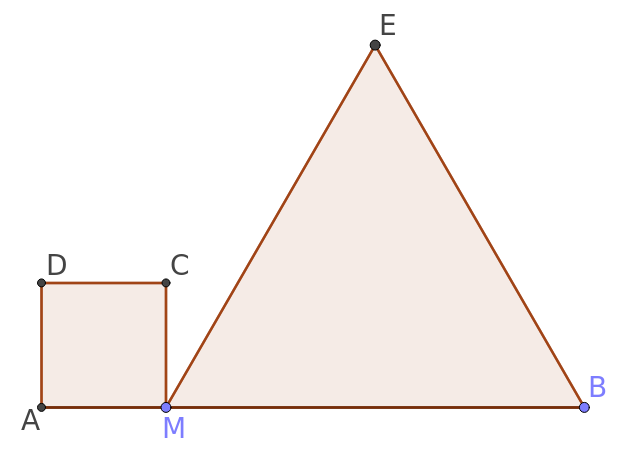
\includegraphics[width=0.3\textwidth]{image/calcul/pbtricar1.png}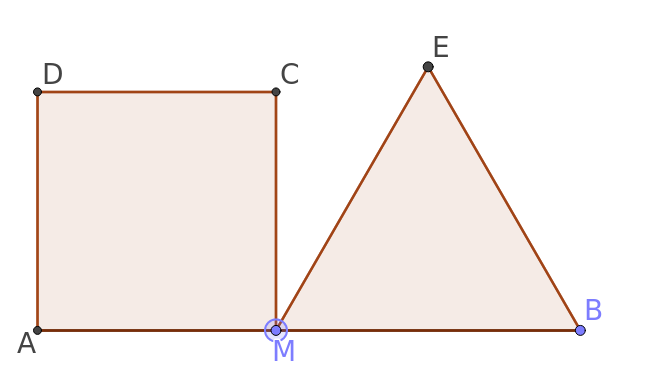
\includegraphics[width=0.3\textwidth]{image/calcul/pbtricar2.png}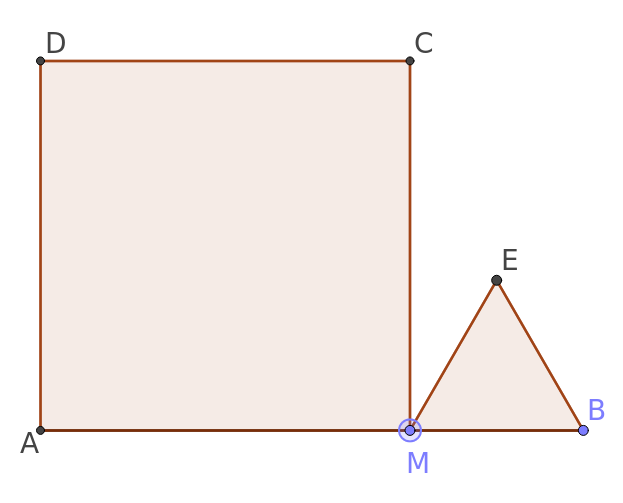
\includegraphics[width=0.3\textwidth]{image/calcul/pbtricar3.png}

	\emph{Début de la réponse.}
	Notons $d$ la distance $AM$. Le périmètre du carré mesure $P_c=4\times AM=4\times d = 4d$. 
	Notons $d'$ la distance $MB$. Le périmètre du triangle mesure $P_t=3\times MB = 3\times d'=3d'$. Mais on a $d+d'=1$ donc nécessairement, $d'=1-d$. Ainsi, $P_t=3\times(1-d)$. Pour égaliser les périmètres, il suffit d'écrire que $P_c=P_t$. En substituant avec les expressions trouvées, il faut donc placer le point $M$ à la distance $d$ du point $A$, où le nombre $d$ vérifie l'égalité suivante :
	\begin{equation}
		4d=3(1-d).
	\end{equation}
	Cette égalité dans laquelle figure un nombre inconnu représenté ici par la lettre $d$ s'appelle une {\bfseries équation}. On appelle \emph{résoudre une équation} l'action de trouver tous les nombres inconnus qui réalisent cette égalité.

	\paragraph{Problème B} Un automobiliste se déplace avec une vitesse $v$ pour parcourir une distance $d$ (par exemple, un chauffard roule à $v=$160km/h pour faire Paris-Toulouse en voiture, $d\approx 630$km). Quelle sera la durée du trajet\,?

	\emph{Début de la réponse.}
	On sait que la vitesse est la proportion de distance parcourue par rapport à un temps donné : si pendant une même durée je parcours une plus grande distance, alors je vais plus vite\,; de même, si je parcours la même distance pendant une durée plus courte, alors je vais plus vite. Ainsi, un mobile qui parcourt la distance $d$ pendant la durée $d$, a une vitesse qui vérifie l'égalité suivante\,:
	\begin{equation}
		v=\frac{d}{t}.
	\end{equation}
	Dans le problème B, la vitesse et la durée sont données, et nous cherchons la durée. Il s'agit d'isoler la durée et de l'exprimer en fonction des deux autres grandeurs, on aimerait secouer cette équation jusqu'aboutir à quelque chose de la forme \og{}$v=\ldots$\fg. 

\chapter{Théorie du produit en croix}\label{chap_croix}
	\section{(R)appel : classe d'équivalence}
		\initial{L}{a} mathématique, c'est la théorie abstraite des relations entre des quantités (par \guil{quantité} j'entends évidemment les nombres, mais aussi des objets potentiellement plus abstraits qui généralisent les nombres, ou même, des objets géométriques). La notion de relation en mathématiques est donc fondamentale. La relation la plus utile et la plus simple, c'est l'égalité. Mais il y en a d'autres. Par exemple, le parallélisme entre deux droites est aussi une relation entre deux objets. Bref, tout n'est que relation univoque entre objets dans cette discipline. Mais une relation sans contenu est vide. Donc, on commence toujours par décrire l'espace général dans lequel on travaille afin de savoir de quoi on parle, avant d'en parler. Par exemple : est-ce qu'on travaille avec des objets géométriques dans le plan d'Euclide, est-ce qu'on travaille sur des nombres\,? et bien d'autres cas possibles. Pour généraliser tout cela, on peut noter cet \guil{espace général} comme un ensemble $E$ qui contient des éléments $a$, $b$, $c$, etc. La plupart des \guil{phrases} écrites en symboles mathématiques commenceront donc par \guil{$\forall a, b, c,\ldots \in E,\ldots$} ce qui peut se traduire par\footnote{en guise de dico\,: $\forall=$\guil{pour tout}, $\in$=\guil{appartient à} ou \guil{appartenant à} ou autre conjugaison, selon le contexte.} \guil{pour tous $a$, $b$, $c$ et éventuellement autres éléments appartenant à l'ensemble $E$, on a\ldots}.

		Ainsi, si par exemple l'on travaille dans l'ensemble des nombres entiers naturels $\N$, on aura $E=\N$, et ses éléments seront les nombres entiers. Dans le cas général, si l'on note une relation générique $R$, alors on dit que deux éléments $a$ et $b$ dans l'ensemble $E$ sont en relation $R$ en notant tout simplement $aRb$. Si l'on veut dire que $R$ est l'égalité, et qu'on remplace $a$ par $1+1$ et $b$ par $2$, alors la phrase \guil{$aRb$} devient tout simplement \guil{$1+1=2$}. On peut aussi penser à la relation \guil{strictement inférieur}, notée $<$. Si l'on remplace $a$ par $1$ et $b$ par $2$, on obtient tout simplement la phrase \guil{$1<2$}.

		\begin{defi}
			Soit $R$ une relation dans un ensemble $E$. On dit que $R$ est une relation d'équivalence lorsque elle vérifie les propriétés suivantes\footnote{Exercice\,: traduire en français les trois points de la définition\,!}\,:
			\begin{itemize}[$\bullet$]
				\item Réflexivité\,: $\forall a\in E, aRa$.
				\item Symmétrie\,: $\forall a,b\in E, aRb\Rightarrow bRa$.
				\item Transitivité\,: $\forall a,b,c\in E, (aRb\wedge bRc)\Rightarrow aRc$. 
			\end{itemize}
		\end{defi}

		On peut vérifier très rapidement que l'égalité est bien une relation d'équivalence. Mais c'est aussi vrai pour le parallélisme (en admettant que deux droites identiques constituent un cas particulier de droites parallèles). Pour ceux qui ont suivi le cours sur le théorème de Thalès : la semblabilité de triangles (et donc de figures géométriques) est une relation d'équivalence. En revanche, la relation $<$ n'est pas une relation d'équivalence. En effet, on a $1<2$ mais on ne peut pas les échanger\,: $2<1$ est faux. Donc la réflexivité est contredite.


		\begin{defi}
			Soit $R$ une relation d'équivalence dans un ensemble $E$ et soit $e\in E$. La classe d'équivalence qui a pour représentant $e$, souvent notée $\bar{e}$, est l'ensemble des éléments qui sont en relation avec $e$. On note de manière compacte\,:
			\begin{equation}
				\bar{e}=\{x\in E | eRx\}.
			\end{equation}
		\end{defi}


		Ici, l'égalité perd un peu son intérêt, car il y a identité entre le représentant d'une classe et sa classe elle-même. En effet, l'ensemble des nombres égaux à 2, c'est... 2. Le parallélisme offre quelque chose de plus intéressant. En effet, si l'on se donne une droite, il existe une infinité de droites qui lui sont parallèles, et elles recouvrent même l'intégralité du plan. La classe d'équivalence de toutes ces droites, en fait, donne la notion de \emph{direction}\,: c'est en quelque sorte le degré d'inclinaison de la droite dans le plan, qui est commun à toute cette infinité de droites.

		%Remarque\,: parfois, pour éviter des ambiguïtés, on note $e/E$ au lieu de $\bar{e}$, afin de savoir dans quel ensemble global se place la classe d'équivalence. En effet, si l'ensemble $E$ est contenu dans l'ensemble $F$, alors $e/E$ n'est pas nécessairement la même chose que $e/F$, et alors la notation $\bar{e}$ pourrait présenter une ambiguïté. Exemple : si l'on considère une droite, selon que l'on considère cette même droite appartenant à un plan ou appartenant à l'espace à trois dimensions, alors on comprend bien que la classe d'équivalence du parallélisme dont le représentant est cette droite n'est pas la même, selon que l'on est dans le plan ou dans l'espace.


	\section{Fondements de la théorie}\label{sec_fond}
		La théorie du produit en croix que je propose est en opposition totale avec le vomi académique qui propose de retenir des recettes magiques de calculs de \guil{quatrième proportionnelle} à l'aide de signes sataniques sortis du chapeau du professeur. Nous allons proposer une théorie axiomatique puis déductive du produit en croix. Il s'agit simplement de définir les fractions comme représentants d'une classe d'équivalence, le quotient de deux nombres --- c'est-à-dire le résultat de leur division.
		\begin{axi} (Loi du produit en croix)
			Soient $a$, $b$, $c$, et $d$ quatre nombres (réels). Alors\,:
			\begin{equation}
				\boxed{\frac{a}{b}=\frac{c}{d} \Leftrightarrow ad=bc}
			\end{equation}
			Autrement dit, si $a$ et $b$ sont deux nombres, on définit le quotient $\frac{a}{b}$ comme la classe d'équivalence des couples de nombres $(c;d)$ tels que $ad=bc$. En langage plus formel, si $\mathbb{E}$ est un ensemble de nombre, on écrit, sous réserve d'existence\,:
			\begin{equation}
				\frac{a}{b}=\left\{ (c,d)\in\mathbb{E}^2|ad=bc\right\}			
			\end{equation}
		\end{axi}

		Toute cette artillerie lourde peut vous paraître compliquée à comprendre en première lecture. Nous allons expliciter cet axiome avec différents niveaux de lecture.
		\begin{enumerate}
			\item Niveau 0. \\ Déjà, il s'agit d'un axiome. Nous ne le démontrerons pas. Il s'agit du point de départ de notre théorie. 
			\item Niveau 1. \\ Pour passer de gauche à droite dans l'égalité de l'axiome, on constate que l'on a écrit le produit des nombres aux extrémités d'une croix qui remplacerait le signe égal. On pourrait donc renommer cet axiome\,: égalité des produits croisés. D'où le fameux nom \guil{produit en croix}.
			\item Niveau 2. \\ Ce qu'il faut comprendre, c'est que $q=a/b$ est le résultat de la division de $a$ par $b$. On peut démontrer à partir de l'axiome que $q$ est l'unique nombre véfifiant $qb=a$. En effet, puisque diviser par 1 ne change pas le résultat, on peut écrire que $q/1=a/b$, et en appliquant l'axiome, on trouve que $qb=a\times1=a$. Réciproquement, s'il existait $q$ et $q'$ qui vérifiaient l'égalité $qb=a$, en remarquant que $a=a\times 1$, on trouve que $q/1=a/b=q'/1$ et donc que $q=q'$\,; le résultat de la division de $a$ par $b$ est donc bien unique grâce à cet axiome.
			\item $(\star)$ Niveau 3. La notion de classe d'équivalence permet de faire une distinction entre le quotient et la fraction. Le quotient est un nombre, c'est le résultat unique d'une division. Mais cette division en tant qu'opération n'est pas unique. Ainsi, la fraction apparaît comme une écriture possible du quotient. Lorsque l'on écrit par exemple $2/3$ en tant qu'écriture, on laisse l'opération en attente, sans l'effectuer. Et donc $2/3$ en tant que fraction n'est pas égale à $4/6$. Mais si on considère $2/3$ en tant que quotient, alors on sous-entend que même si le résultat de l'opération de division n'est pas explicitement écrit, il est sous-entendu par l'écriture. Et alors, on peut bien écrire que $2/3=4/6$, les quotients précédents étant considérés en tant que nombres. D'ailleurs, on peut utiliser l'axiome pour vérifier cette égalité\,: en effet, on a bien $2\times6=3\times4$. Ici on a écrit que $2/3=4/6$, mais en vérité il y a une infinité de quotients qui sont égaux à $2/3$\,: $4/6;\;6/9;\;8/12;$ etc. Bref, l'ensemble de toutes les fractions $c/d$ où les nombres $c$ et $d$ ont été choisis de manière à ce que $2\times d=3\times c$.  
		\end{enumerate}

		$(\star)$ \emph{Jusqu'à la section \ref{sec_regles}, ce qui suit peut être sauté en première lecture.}

		À titre de remarque préliminaire, une fois que l'on a défini le quotient, il convient de définir l'inverse d'un nombre.
		\begin{defi}
			Soit $a$ un nombre. Sous réserve d'existence, $b$ est un inverse de $a$ si $a\times b=b\times a=1$. On notera alors $b=1/a$.
		\end{defi}
		\begin{thm}
			L'inverse d'un nombre est unique.
		\end{thm}
		\begin{proof}
			Soient $b$ et $b'$ deux inverses de $a$. Alors $ab=ab'=1$. D'après l'axiome, on a $b=1/a=b'$.
		\end{proof}
		\begin{cor}
			Diviser par un nombre revient à multiplier par son inverse.
		\end{cor}
		\begin{proof}
			Supposons que $q=\frac{a}{b}$, alors $qb=a$. Considérons le nombre $a\times1/b$. Alors on a $a\times 1/b\times b=a\times 1 =a$ car multiplier par $b$ est l'opération réciproque de diviser par $b$. Par unicité du quotient, on a bien $a/b=a\times 1/b$.
		\end{proof}

		Souvent, vos professeurs de mathématiques vous ont hurlé dessus ou ont eu des crises cardiaques lorsque vous avez divisé un nombre par zéro. Le théorème suivant explique pourquoi.
		\begin{thm}
			0 n'a pas d'inverse.
		\end{thm}
		\begin{proof}
			Si zéro avait un inverse, alors il existerait un nombre $x$ tel que $0\times x=1$, mais pour tout nombre $x$, $0\times x=0$ et donc on aurait $1=0$, ce qui est absurde.
		\end{proof}


	\section{Quelques règles de calcul utiles}\label{sec_regles}
		Voici quelques règles de calculs fort utiles pour manipuler des expressions algébriques\,:
		\begin{thm}
			Soient $a$,$b$,$c$,$d$ des nombres tels que les dénominateurs apparaissants plus bas soient non nuls. Alors les opérations élémentaires s'effectuent de la manière suivante\,:
			\begin{itemize}[$\bullet$]
				\item simplification des fractions\,:
				\begin{equation}
					\frac{a}{b}=\frac{a}{b}\times\frac{d}{d}=\frac{ad}{bd};
				\end{equation}
				\item multiplication d'un quotient par un nombre\,:
				\begin{equation}
					\frac{a}{b}\times c=\frac{ac}{b};
				\end{equation}
				\item multiplication et division de deux quotients\,:
				\begin{equation}
					\frac{a}{b}\times\frac{c}{d}=\frac{ac}{bd};\quad \frac{\frac{a}{b}}{\frac{c}{d}}=\frac{a}{b}\times\frac{d}{c}=\frac{ad}{bc};
				\end{equation}
				pour la dernière série d'égalités, on remarque que diviser par un nombre revient à le multiplier par son inverse. Notamment\,:
				\begin{equation}
					\frac{\frac{a}{b}}{c}=\frac{a}{b}\times\frac{1}{c}=\frac{a}{bc};
				\end{equation}
				\item addition ou soustraction de deux quotients, selon qu'ils aient ou non le même dénominateur\,:
				\begin{equation}
					\frac{a}{b}\pm\frac{c}{b}=\frac{a\pm c}{b};\quad \frac{a}{b}\pm\frac{c}{d}=\frac{ad\pm bc}{bd}.
				\end{equation}
			\end{itemize}
		\end{thm}
		\begin{proof}
			Ce sont des démonstrations élémentaires du même type que les démonstrations de la section \ref{sec_fond} (ah\,! je vois déjà les petits malins qui ont sauté les passages difficiles\,! Vous voilà bien embarrassés maintenant.). Elles sont amusantes à faire, à petite dose. C'est la raison pour laquelle je les laisse en exercices. Si vous êtes capables d'en faire quelques unes, cela signifie que vous avez compris la méthode, ce qui est le plus important.
		\end{proof}

		Remarque : pour la dernière égalité du théorème, en pratique il s'agit de réduire les deux fractions à ajouter/soustraire au même dénominateur afin de pouvoir effectuer l'opération avec les numérateurs. En général on ne va pas utiliser exactement cette égalité, mais on va simplifier directement en cherchant le diviseur commun le plus grand entre les deux dénominateurs\footnote{($\star$) En fait, tout ceci pourrai s'écrire formellement ainsi\,:
		\begin{equation}
			\frac{a}{b}\pm\frac{c}{d}=\frac{\frac{ad}{\mathrm{pgcd}(b,d)}\pm \frac{cb}{\mathrm{pgcd}(b,d)}}{\mathrm{ppcm}(b,d)}
		\end{equation}.}. Prenons un exemple\,:
		\begin{equation}
			\frac{1}{6}-\frac{2}{9}=\frac{1\times 3}{6\times 3}-\frac{2\times 2}{9\times 2}=\frac{3}{18}-\frac{4}{18}=-\frac{1}{18}.
		\end{equation}

		À présent, il convient de résoudre un problème classique. Imaginons que sur les quatre nombres $a$, $b$, $c$, $d$, trois soient donnés et qu'on cherche le quatrième, sachant que $a/b=c/d$. C'est ce qu'on appelle le problème du produit en croix. Je pourrais donner un théorème général qui donnerait toutes les solutions possibles, mais il est plus intéressant que le lecteur cherche lui-même la solution.


	\paragraph{Exercices}
	\begin{enumerate}
		\item Résoudre les équations suivantes (trouver le nombre inconnu en fonction des nombres connus) : $\frac{1}{x}=\frac{2}{3}$ ; $\frac{3}{4}=\frac{2}{y}$. Pour procéder, on utilisera d'abord l'axiome du produit en croix, puis on divisera les deux membres de l'égalité par le nombre qui multiplie l'inconnue afin de s'en débarrasser par simplification d'une fraction.

		\item On suppose que $\frac{a}{b}=\frac{c}{d}$. Exprimer chacun des quatre nombres en fonction des trois autres\footnote{Cela signifie qu'on veut écrire\,: $a=\ldots$, puis $b=\ldots$, etc. où les points de suspension contiennent une expression qui dépendent des trois autres nombres que celui à gauche du signe égal.}.

		\item Résoudre le problème B.
	\end{enumerate}

	\emph{Solutions\,:}
	\begin{enumerate}
		\item $\frac{1}{x}=\frac{2}{3} \Leftrightarrow 1\times 3 = 2\times x$ d'après l'axiome. En simplifiant, on écrit donc que $2x=3$. Mais on ne cherche pas $2x$, on cherche $x$. Ainsi, puisqu'on a $2$ fois trop de $x$, on va diviser les deux côtés de l'égalité par 2 (afin de ne pas déséquilibrer l'égalité). Ce qui donne donc\,: $\frac{2x}{2}=\frac{3}{2}$. Mais d'après la règle de simplification des fractions, on a simplement $x=\frac{3}{2}$. Et donc la solution est $\frac{3}{2}$. 

		En général, on ne s'embarrasse pas d'une rédaction aussi lourde. Pour résoudre la deuxième, on écrira utilement\,:
		\begin{equation}
			\frac{3}{4}=\frac{2}{y} \Leftrightarrow 3\times y = 2\times 4 \Leftrightarrow \frac{3y}{3}=\frac{8}{3} \Leftrightarrow y=\frac{8}{3} \nonumber
		\end{equation}
		et donc la solution est $8/3$.

		Avec un peu de pratique, on peut même le faire en une étape, "de tête".

	\item Avec la même méthode, on peut trouver que $\frac{a}{b}=\frac{c}{d}\Leftrightarrow a=\frac{bc}{d}$. Les autres sont laissées au lecteur.
	\item On trouve $t=d/v$, et si on remplace par les valeurs, on trouve donc $t=630$(km)$/160$(km/h)$\approx 4$h.

	\end{enumerate}
	
\chapter{Équations du premier degré}\label{chap_eqp}
	\section{Résolution algébrique pure}
		On parle de premier degré lorsque l'inconnue (par exemple $x$) intervient en quelque sorte directement dans l'équation\,: soit multipliée par un nombre, soit toute seule. Cependant, on n'admettra pas que l'inconnue apparaisse sous la forme $x\times x$ ou sous la forme $1/x$. En fait, on peut montrer que toutes les équations du premier degré peuvent se mettre sous la forme $ax+b=0$ où $a$ et $b$ sont des nombres quelconques. 

		\begin{axi} (Conservation des quantités)
			Pour tous nombres $a$, $b$, et $c$,
			\begin{equation}
				a+b=c \Leftrightarrow a=c-b.
			\end{equation}
			Autrement dit, si à deux quantités égales, on ajoute ou on retranche la même quantité, alors les résultats obtenus seront égaux.\item{On trouve cet axiome dans l'ouverture des \emph{Éléments} d'Euclide.}
		\end{axi}

		On rappelle que par convention, $ab+c=(ab)+c$. Dans les livres communs de l'enseignement secondaire, on appelle cela la \emph{priorité de la multiplication (ou de la division) sur l'addition (ou la soustraction)}. Nous préférons dire, comme Stella Baruk, que le nombre $(ab)+c$ est globalement une somme\,: la somme de $ab$ et de $c$. Autrement dit, l'opération globale à effectuer est une addition. L'addition donc l'opération qu'il faudra effectuer en dernier, une fois qu'on aura intégralement déterminé ses termes à additionner, $ab$ et $c$. 

		\paragraph{Exercice 1} Résoudre les équations suivantes, c'est-à-dire, trouver le nombre inconnu (désigné par une lettre) qui réalise l'égalité.
		\begin{enumerate}
			\item Ceinture rose
			\begin{equation}
			 	x+1=2;\quad 2y=4;\quad 2y+3=5.
			\end{equation} 
			\item Ceinture blanche
			\begin{equation}
				5z-2=3;\quad 2u-1=9.
			\end{equation}
			\item Ceinture jaune
			\begin{equation}
				3u-2=0;\quad 3v+2=0
			\end{equation}
			\item Ceinture verte
			\begin{equation}
				2w+5=5w-4
			\end{equation}
			\item Ceinture rouge
			\begin{equation}
				\frac{2}{3}x-\frac{5}{6}=-\frac{9}{11}x+\frac{7}{13}
			\end{equation}
		\end{enumerate}

	\section{Approfondissement\,: résolution dans un ensemble}

		Nous déjà avons vu quelques ensembles de nombres\,: $\N$, $\Z$, $\D$, et $\Q$ (voir annexe \ref{app_nbs} pour des rappels).
		En fait, lorsqu'on cherche à résoudre une équation, on cherche un nombre dans un ensemble défini à l'avance. Ce point est d'une très grande importance car cela peut changer l'existence ou non d'une solution. Voici un petit exemple/contre-exemple très classique\,:
		Résoudre l'équation suivante sachant que $x\in \N$ : $2x=1$. En divisant par deux cette égalité, on trouve que
		\begin{equation}
			2x=1 \Leftrightarrow x=\frac{1}{2} 
		\end{equation}

		Cette ligne signifie : \guil{dire que $2x=1$ est équivalent à dire que $x=1/2$}. C'est un raisonnement par équivalence. Cependant, dire qu'une proposition équivaut à une autre ne veut pas dire que l'une ni l'autre soit vraie. Surtout si l'on se rappelle qu'on avait exigé que $x$ soit un nombre entier naturel. En effet, $2x=1$ c'est la même chose que $x=1/2$, soit $0.5$ en écriture décimale. Mais ceci entre en contradiction avec l'exigence de départ : que $x$ soit un entier naturel. Ainsi, puisque l'équation équivaut à quelque chose d'impossible (que $x=0.5$ \emph{et en même temps} que $x\in\N$), alors on concluera que l'équation n'a pas de solution dans $\N$. On écrira alors que l'ensemble des solutions, noté $S$ par convention, est vide. Cet ensemble est représenté par le symbole $\emptyset$ en mathématiques. Voici donc comment on rédige tout ce raisonnement en symboles mathématiques\,:
		\begin{equation}
		 	2x=1\Leftrightarrow x=\frac{1}{2}=0.5\notin\N ; \quad S=\emptyset.
		\end{equation} 
		En revanche, si l'on souhaite résoudre cette équation dans un ensemble de nombres plus \guil{gros}, par exemple l'ensemble des nombres décimaux, alors on écrira\,:
		\begin{equation}
		 	2x=1\Leftrightarrow x=\frac{1}{2}=0.5\in\D ; \quad S=\{0.5\}.
		\end{equation} 
		J'attire votre attention sur la notation $S=\{0.5\}$\,: $S$ n'est pas un nombre, c'est un ensemble de nombres, celui qui contient le nombre $0.5$. Cela sera utile lorsque certaines équations contiendront plus qu'une seule solution. 
		Nous alons en construire une immédiatement. Nous avons besoin d'un théorème\,:
		\begin{thm}
			Un produit de facteurs est nul si et seulement si au moins l'un des facteurs est nul. Autrement dit, si $a,b,c,\ldots$ sont des nombres, alors\,:
			\begin{equation}
				abc\ldots = 0 \Leftrightarrow(a=0\lor b=0 \lor c=0\lor \ldots).
			\end{equation}
		\end{thm}

		\begin{proof}
			$\Leftarrow$ immédiat par propriété de la multiplication par zéro.

			$\Rightarrow$ raisonnement par contraposée. Si aucun des facteurs n'est nul, alors leur produit est non nul.
		\end{proof}

		Ainsi, résolvons par exemple dans $\R$ l'équation $(x+1)(x-1)=0$. On écrira\,:
		\begin{equation}
			(x+1)(x-1)=0 \Leftrightarrow (x+1=0\lor x-1=0) \Leftrightarrow (x=-1\lor x=1); \quad S=\{1;-1\}.
		\end{equation}
		(Nous n'avons pas précisé qu'ici, $1$ et $-1$ sont des nombres réels car cela ne présentait pas d'ambiguïté). Ici, l'ensemble solution est un ensemble qui contient non pas un, mais deux nombres. 

		Voyons un cas encore plus tordu. Essayons de résoudre, par exemple dans l'ensemble $\Q$, l'équation $r=r$. En fait, cette égalité est vraie pour tout nombre rationnel $r$, donc tous les nombres de l'ensemble $\Q$ sont solutions. L'ensemble solution n'est autre que $\Q$ lui-même\,: $S=\Q$\,!

		Et tentons de résoudre $z=z+1$ dans l'ensemble $\R$. Avec un peu d'intuition, on peut voir qu'il n'existe aucun nombre $z$ vérifiant cette égalité, mais une fois n'est pas coutûme, faisons les automathes avec un raisonnement par l'absurde\,: supposons qu'il existe un nombre réel $z$ qui vérifie l'égalité escomptée. Alors, en soustrayant $z$ des deux côtés, on obtient\,: $z-z = z+1-z$, et en simplifiant, on obtient\,: $0=1$. Cette égalité étant absurde, nous devons contredire l'hypothèse qui y a menée, et donc, il n'y a pas de solution\,: $S=\emptyset$.






	\section{Résolution graphique}

		\subsection{Repère cartésien}
			Descartes a démocratisé le lien entre la géométrie et l'algèbre, avec ce qu'on appelle aujourd'hui les \emph{repères cartésiens}. Nous allons  présenter le repère le plus utile qui soit, le repère cartésien orthogonal. Nous utiliserons une présentation semi-intuitive comme celle de Descartes\footnote{La théorie axiomatique des nombres réels sera abordée dans une future leçon.}.

			Considérons une droite. Plaçons un point arbitraire $O$ sur cette droite, ainsi qu'un autre point arbitraire nommé $I$. Le premier point sera appelé {\bfseries l'origine} du repère alors que le deuxième point permettra de définir {\bfseries l'unité de mesure des distance}. En effet, nous venons de créer une unité de mesure, et nous poserons que la distance $OI$ sera égale à l'unité.
			Une telle droite a plusieurs noms dans les livres de mathématiques; pour l'heure nous la nommerons \emph{droite graduée}.

			Plaçons un point $A$ de manière arbitraire sur la droite. Nous allons définir de manière unique un nombre qui permettra de repérer ce point sur la droite. Ce nombre, souvent noté $x$, est l'abscisse du point $M$. Il est défini comme suit\,:
			\begin{itemize}[$\bullet$]
				\item Si $M$ est du même côté que\footnote{La notion \guil{du même côté que} sera définie formellement dans le chapitre de trigonométrie.} $I$ par rapport à $O$, $x=\frac{OM}{OI}$ (illustration ci-dessous).

				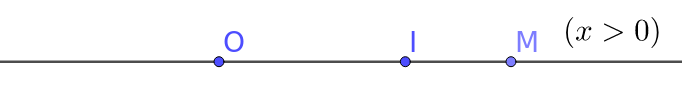
\includegraphics[width=0.6\textwidth]{image/calcul/point1d1.png}
				\item Sinon, $x=-\frac{OM}{OI}$ (illustration ci-dessous). 

				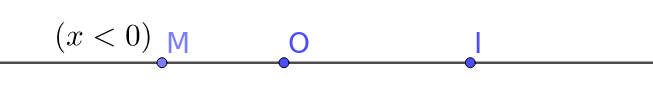
\includegraphics[width=0.6\textwidth]{image/calcul/point1d2.png}
			\end{itemize}



			En deux dimensions, il faut ajouter un deuxième axe qui coupe le premier. Le plus simple est de prendre un axe perpendiculaire au premier, qui le coupe en $O$. Ensuite, nous choisissons un point $J$ tel que $OI=OJ$ pour avoir la même unité de mesure dans les deux axes\footnote{Ce n'est pas une obligation. Les deux axes pourraient même avoir des origines différentes. Mais nous commençons par présenter le cas le plus simple.}. Un tel repère est appelé \emph{Repère orthonormé}. Si nous choisissons de mettre le point $I$ \guil{vers la droite} et le point $J$ \guil{vers le haut}, on dit que le repère est \emph{direct}, sinon il est \emph{indirect}\footnote{Il s'agit de l'orientation du repère. Plus rigoureusement\,: si les points $O$, $I$, $J$, dans cet odre, tournent dans le sens anti-horaire, alors le repère est direct. Sinon il est indirect. L'orientation sera définie formellement dans le chapitre de trigonométrie.}. Ayant construit une deuxième droite graduée, on peut y placer un autre point, $B$ également repréré par une autre abscisse, le nombre $y$. Mais en général, pour le deuxième axe, on préfère parler d'\emph{ordonnée} plutôt que d'abscisse, afin d'éviter de confondre les deux. 
			Muni de ces deux nombres $(x,y)$, on peut construire un point du plan, le point $M$, qui sera l'unique point tel que $OAMB$ est un rectangle. 

			Réciproquement, si l'on se donne un point du plan $M$, alors on pourra trouver de manière univoque son abscisse $x$ et son ordonnée $y$. Pour ce faire, il suffit de tirer la droite perpendiculaire à $(OI)$ passant par $M$\,; cette droite coupe $(OI)$ en $A$ et $x$ n'est autre que l'abscisse de $A$. De même pour $y$ en prenant la perpendiculaire à $(OJ)$ passant par $M$.

			Les nombres $(x,y)$ regroupés dans un couple sont les {\bfseries coordonnés cartésiennes} du point $M$.

			Nous  illustrons cela ci-dessous\,:

			\vspace{0.2cm}

			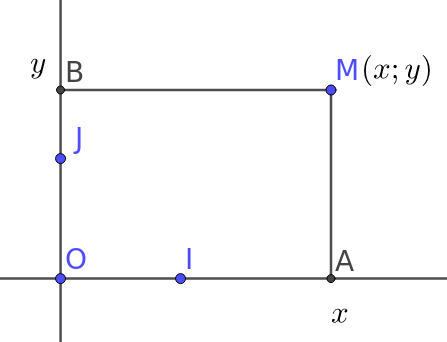
\includegraphics[width=0.4\textwidth]{image/calcul/point2d.png}			

			Notez que d'après le théorème de Pythagore, si le point $M$ est repéré par les coordonnées $(x,y)$ et $N$ par les coordonnées $(x',y')$, alors la distance $MN$ se calcule ainsi\,:
			\begin{equation}
				MN=\sqrt{(x-x')^2+(y-y')^2}
			\end{equation}

			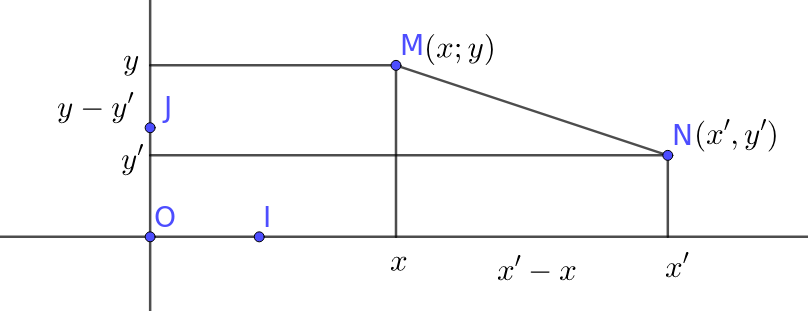
\includegraphics[width=0.7\textwidth]{image/calcul/point2dpyth.png}


		\subsection{Courbe d'une fonction}
			Maintenant que nous savons repérer un point quelconque dans le plan, imaginons que nous fassions varier $x$ et $y$ continument dans le temps. Imaginons que le point $M$ soit au préalable plongé dans de l'encre et qu'il laisse une trace. Alors le résultat sera une ligne tracée sur le plan, que l'on a coutûme d'appeler \emph{courbe}\footnote{Bien qu'elle ne soit pas forcément courbée. Ainsi, les droites sont aussi des \guil{courbes}\,!}. Il existe de nombreuses façons de construire des courbes et nous ne les aborderons pas toutes. La manière la plus simple de construire des courbes est de considérer que les quantités $x$ et $y$ ont une relation de dépendance, et en particulier, que $y$ dépend de $x$. On écrira que $y=f(x)$, sous-entendu, que $y$ est fonction de $x$. Notez que $f(x)$ se lit \guil{$f$ de $x$} (le choix de la lettre $f$ correspond au mot \guil{fonction}, mais il est possible de prendre n'importe quelle autre lettre). De là, il suffit de faire varier le nombre $x$ et, pour chaque valeur connue de $x$, il suffit de calculer le nombre $y$ correspondant. On obtient un tableau qui regroupe de nombreuses coordonnées du point mobile, et il suffit de les tracer et de les relier plus ou moins continument pour obtenir quelque chose qui ressemble à une courbe.

			Essayons par exemple de tracer la courbe dont les coordonnées vérifient $y=x^2$. Ici, nous avons donc $c(x)=x^2$ (le choix de la lettre $c$ vient du fait que le processus de cette fonction consiste à élever le nombre $x$ en son carré, $x^2$). En théorie, $x$ varie de moins l'infini jusqu'à plus l'infini, mais la taille du papier n'étant pas infinie, nous allons restreindre le domaine de variation du nombre $x$. Nous partirons de $x=-2$ et nous irons jusqu'à $x=+2$ par exemple. Alors, il faut remplir le tableau suivant\,:

			\begin{tabular}{|c|c|c|c|c|c|c|c|c|c|c|}
				\hline
				$x$     &$  -2 $&$ -1.8 $&$ -1.6 $&$ -1.4 $&$ -1.2 $&$ -1 $&$ -0.8 $&$ -0.6 $&$ -0.4 $&$ -0.2 $\\
				\hline
				$y=x^2$ &       &         &       &        &        &      &         &       &         &        \\
				\hline
			\end{tabular}

			\vspace{0.3cm}

			\begin{tabular}{|c|c|c|c|c|c|c|c|c|c|c|c|}
				\hline
				$x$     &$  0 $&$ 0.2    $&$ 0.4 $&$ 0.6  $&$ 0.8  $&$ 1   $&$1.2    $&$ 1.4 $&$ 1.6   $&$ 1.8  $& 2\\
				\hline
				$y=x^2$ &       &         &       &        &        &      &         &       &         &        & \\
				\hline
			\end{tabular}

\iffalse

			\begin{tabular}{|c|c|c|c|c|c|c|c|c|c|c|}
				\hline
				$x$     &$  -2 $&$ -1.8 $&$ -1.6 $&$ -1.4 $&$ -1.2 $&$ -1 $&$ -0.8 $&$ -0.6 $&$ -0.4 $&$ -0.2 $\\
				\hline
				$y=x^2$ &   4   & $3.24$ &$2.56$  &$1.96$  &$ 1.44$ & $1$  &$0.64$  &$0.64$  &$0.16$  &$0.04$   \\
				\hline
			\end{tabular}

			\vspace{0.3cm}

			\begin{tabular}{|c|c|c|c|c|c|c|c|c|c|c|c|}
				\hline
				$x$     &$  0 $&$ 0.2    $&$ 0.4 $&$ 0.6  $&$ 0.8  $&$ 1   $&$1.2    $&$ 1.4 $&$ 1.6   $&$ 1.8  $& 2\\
				\hline
				$y=x^2$ &$0$   &$0.04$    &$0.16$ &$0.36$  &$0.64$  &$1$    &$1.44$   &$1.96$ &$2.56$   &$3.24$  &$4$ \\
				\hline
			\end{tabular}
\fi


			Pour la première case vide, il faut effectuer le calcul suivant en remplaçant $x$ par la valeur annoncée\,: $y=x^2=(-2)^2=(-2)\times(-2)=+4$. Et ainsi de suite pour toutes les autres cases. Souvent, on utilise des logiciels pour automatiser la procédure. Geogebra le fait automatiquement, et calcule beaucoup plus de valeurs que dans ce simple tableau, ce qui donne l'illusion d'une belle courbe continue. Nous, nous allons utiliser le tableur\,:

			\noindent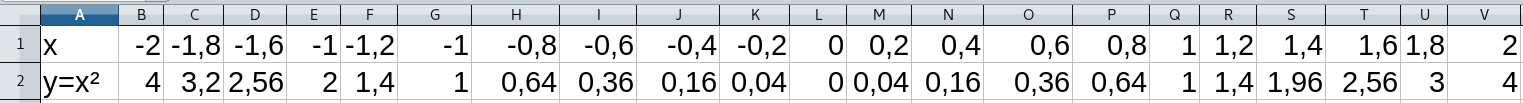
\includegraphics[width=\textwidth]{image/calcul/valfctcar.png}

			Pour obtenir ce tableau, il suffit de rentrer -2 en B1, puis de rentrer en C1\,: \mintinline{python}{=B+0,2} et d'étendre jusqu'à ce qu'on atteigne le nombre 2. Ensuite, il suffit de rentrer en B2 la formule\,: \mintinline{python}{=B1*B1} et d'étendre.

			Nous obtenons alors le \emph{tableau de valeurs de la fonction carré}. Pour tracer ceci, il faut placer chaque couple abscisse/ordonnée dans le plan. Par exemple, lorsque $x=2$, on a $c(x)=4$. Ainsi, il faudra placer un point dont les coordonnées sont $(2;4)$. On fait de même avec les autres points, ce qui donne une idée du graphe de la courbe.

			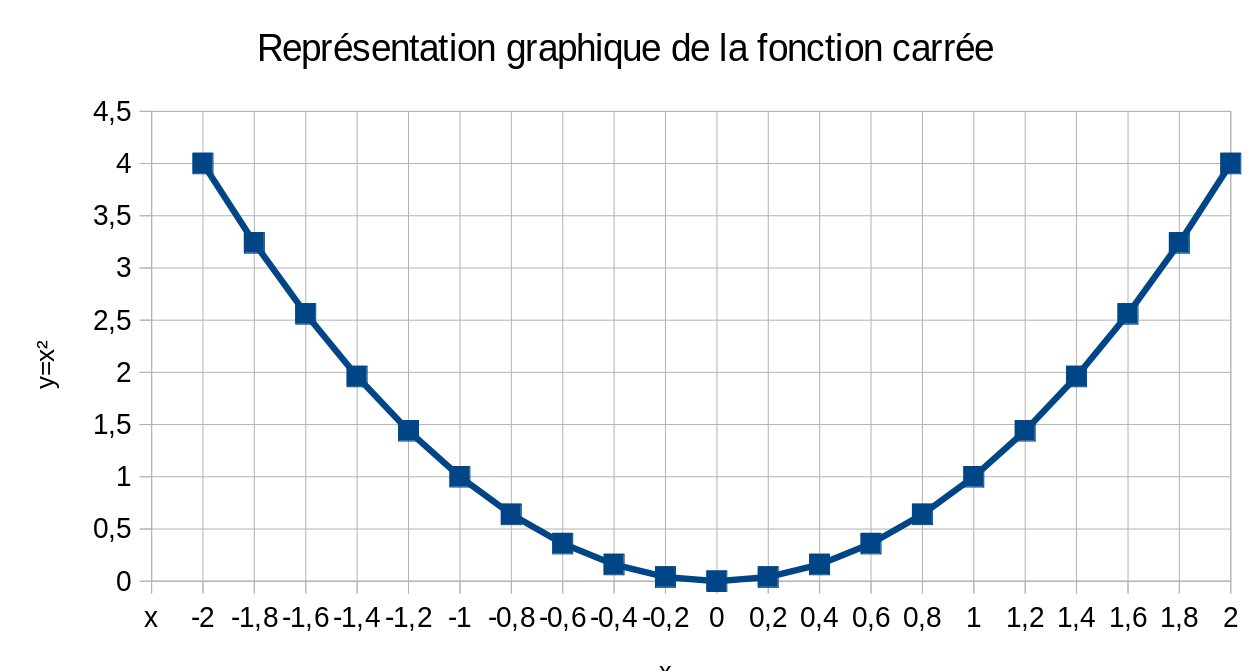
\includegraphics[width=0.9\textwidth]{image/calcul/courbe_fct_car.png}

		\subsection{Modélisation et résolution graphiques d'une équation}

			Une équation du premier degré d'inconnue $x$ peut toujours se mettre sous la forme $f(x)=g(x)$ où $f(x)=ax+b$ et $g(x)=cx+d$ où $a$, $b$, $c$, et $d$ sont des nombres fixés. Si on n'aime pas le calcul, il suffit de tracer les graphes des fonctions $f$ et $g$ et de visualiser où les courbes se coupent. Lorsqu'il y a une unique solution, on a affaire à des droites qui se coupent en un point de coordonnées $(x;y)$. L'abscisse $x$ de ce point est la solution de cette équation. Il suffit donc de lire l'abscisse du point solution sur l'axe des abscisse.

			\paragraph{Exercice 1}
			On considère une voiture sur une autoroute rectiligne se déplaçant à la vitesse $v=130$km/h. On modélise la route par une droite graduée d'origine $O$. La droite est orientée dans le sens du mouvement de la voiture. On note $x(t)$ l'abscisse de la voiture à la date $t$ ; ce nombre représente la position de la voiture sur la droite. On suppose qu'à $t=0$, la voiture passe par $O$.

			\begin{enumerate}
				\item Démontrer que $x(t)=v t$.
				\item Convertir $v$ en m/s.
				\item Compléter le tableau suivant\,:

				\begin{tabular}{c|c|c|c|c|c|c|c|c|c|c|c}
					t (s) & -5 & -4& -3& -2& -1& 0& 1& 2& 3& 4& 5 \\
					\hline
					x(t) (m)& &   &   &    &   &  &  &  &  &  &  
				\end{tabular}

				\item Tracer le graphe de la fonction $x:t\mapsto x(t)$. Commenter cette courbe. Y avait-il besoin d'autant de points que de colonnes dans le tableau précedent pour tracer la courbe\,?
				%\item Calculer l'angle que fait la courbe avec l'axe des abscisses.
				\item Une autre voiture se déplace dans le sens opposé à la première, à la vitesse\\ $v'=110$km/h, et à $t=0$, elle se situe à $d=200$m de la première voiture. On note $y(t)$ son abscisse à la date $t$. Démontrer que $y(t)=-v't+d$. 
				\item Tracer le graphe de la fonction $y$. 
				\item Calculer la date à laquelle les voitures se croiseront. Vérifier la cohérence avec la lecture graphique de la solution.


			\end{enumerate}

			\textit{Solution.} 
			\begin{enumerate}
				\item $v=d/t$ donc $d=vt$.
				\item $1$km$=1000$m et $1$h=$60$min$=60\times 60$s=$3600$s. De là, on tire $1$km/h $=\frac{1\text{km}}{1\text{h}}=\frac{1000\text{m}}{3600\text{s}}=\frac{1}{3.6}$m/s. Donc, 130km/h$=130\times 1/3.6$m/s$\approx 36$m/s.
				\item 

				\begin{tabular}{c|c|c|c|c|c|c|c|c|c|c|c}
					$t$ (s) &$     -5 $&$    -4$&$  -3 $&$   -2 $&$ -1$&$ 0$&$ 1 $&$  2 $&$ 3$&$ 4  $&$ 5 $\\
					\hline
					$x(t)$ (m)&$-180.6 $&$ -144 $&$-108 $&$ -72  $&$-36$&$ 0$&$ 36$&$ 72 $&$108$&$ 144 $& $180.6$ 
				\end{tabular}
				\item La courbe est une droite qui passe par l'origine du repère. Un seul point différent de l'origine aurait suffi à tracer la droite.
				\item On sait qu'à $t=0$, la voiture est à la distance $d$ de la première, dans le sens positif. Donc $y(0)=d$. En suite, la deuxième voiture s'éloigne de cette position à la vitesse $v$, dans le sens négatif, donc l'écart $y(t)-y(0)$ mesure $-v't$. En substituant, cela nous donne $y(t)-d=-vt$, d'où $y(t)=-vt+d$.

			\end{enumerate}


			\paragraph{Exercice 2}
			L'unité de mesure du temps est la seconde, l'unité de mesure des distance est le mètre.

			Le lièvre et la tortue font la course. L'arbitre a un chronomètre qui démarre à $t=0$. La tortue est lente : elle se déplace à $v_T=0.01$m/s. Le lièvre avance à $v_L=20$m/s. 

			On modélise la piste par une demi-droite d'origine $O$ ; la tortue est représentée par un point mobile $T$ et le lièvre est représenté par un point mobile $L$. On note $x_T(t)=OT$, la distance parcourue par la tortue à la date $t$. On note $x_L(t)=OL$, la distance parcourue par le lièvre à la date $t$. 

			La tortue commence la course à $t=0$. Le lièvre, lui, sûr de sa victoire, fait une sieste jusqu'à $t_0=996$s, et\footnote{\emph{Le lièvre et la tortue}, de la Fontaine.}
			\begin{quote}
				[...] à la fin, quand il  vit \\
			  Que l'autre touchait presque au bout de la carrière, \\
			  Il partit comme un trait [...].
			\end{quote}

			\begin{enumerate}
				\item En utilisant les lois de la cinématique, démontrer que lorsque $t\ge0$, $x_T(t)=v_T\times t$.
				\item De même, démontrer que lorsque $0\le t\le 999s$, $x_L(t)=0$ et lorsque $t\ge t_0$s, $x_L(t)=v_L(t-t_0)$.
				\item Tracer le graphe des deux fonctions : $x_T: t\mapsto x_T(t)$, et $x_L:t\mapsto x_L(t)$, pour $0\le t\le 100$s.
				\item Résoudre graphiquement, puis algébriquement, l'équation $x_L(t)=x_T(t)$.
				\item Sachant que la course se déroule sur 100m, qui va gagner ?
			\end{enumerate}









% \include{puissances_racines}

% les balises \iffalse et \fi permettent d'empecher le compilateur de lire ce qu'il y a à l'intérieur. 
% ce sont des balises de commentaires.
% l'idee est de préremplir ce qu'on va mettre pour inclure "maths-champignons" dans ce fichier.
\iffalse
    \part{Géométrie élémentaire semi-intuitive}
    \include{triangle_isom_axiomes_euclide} %Triangles isométriques et axiomes d'Euclide
    \include{mesure_euclide} %Théorie de la mesure d'Euclide : longueurs, aires, volumes.
    \include{pythagore} %Le "vrai" théorème de Pythagore.
    \include{thales} %Le "vrai" théorème de Thalès. Applications : homothéties et triangles semblables.



    \part{Logique mathématique (première partie)}

    \input{import_axiom} % importance de l'axiomatique : contre-exemple de la géométrie sphérique.
    \input{quelques_raisonnements} % Quelques raisonnements mathématiques élémentaires.
    \input{contredire_prop} % Contredire des propositions.
    \input{axiom_rec} % Axiome de récurrence.
\fi

\part{Fugue\,: angles et trigonométrie}\label{part_2}

\chapter{Introduction générale}

Test

\initial{M}{aintenant}\addlb{ que nous nous sommes habitués à manipuler des expressions algébriques, nous allons passer à une branche des mathématiques qui se situe à l'interface entre la géométrie et l'analyse\,: la trigonométrie circulaire. Cette discipline s'occupe d'étudier les mouvements de rotation de manière calculatoire en utilisant une approche cartésienne. Il s'agit d'étudier l'évolution des coordonnées cartésiennes d'un point qui évolue sur un cercle.}

\addlb{Par traditionalisme obsolète, et aussi par une sorte d'\guil{esprit praticiste} qui méprise la théorie, et donc tout ce qui est sérieux en mathématiques, dans \guil{l'école de la confiance de la République des valeurs}, l'unité de mesure des angles est le degré. La confusion empiriste règne, puisqu'on enseigne la notion d'angle d'abord par la mesure d'angle avec le \guil{rapporteur}, comme si c'était un objet magique, et en faisant abstraction de tout le développement théorique qui permet sa construction. En outre, depuis quelques décennies, les programmes de mathématiques de l'Éducation Nationale entretiennent sciemment la confusion entre les secteurs d'angles (lieux géométriques), la mesure des secteurs d'angles (nombres réels), et les angles, intermédiaires entre les deux\,: un angle est l'ensemble des secteurs d'angles qui ont une même mesure donnée. Sous prétexte de ne pas vouloir être trop exigeant avec les élèves, on entretient un brouillard de confusion entre des objets de nature différente. En outre, considérer les jeunes esprits comme incapables de comprendre la mathématique, n'est-ce pas là le mépris le plus effroyable envers ces esprits\,? C'est ce qu'il convient d'appeler \guil{bienveillance}, aujourd'hui, au sein de l'Éducation Nationale\ldots} 

\addlb{Cela va sans dire --- mais va encore mieux en le disant --- notre approche sera radicalement opposée. Nous n'allons pas utiliser l'unité du degré pour les angles, mais son unité naturelle, le radian. Pour le dire vite, l'unité du radian se définit de telle sorte qu'un tour complet correspond à $2\pi$ radian. Le radian est la longueur de l'arc parcouru sur un cercle de rayon unité lorsqu'un point le parcourt selon un mouvement de rotation. Mais pour ce faire, en préambule, nous allons expliquer ce que représente géométriquement le nombre $\pi$, dans une approche semi-intuitive --- l'essentiel des résultats sera démontré, mais nous admettrons les théorèmes classiques qui permettent de faire les démonstrations. La plupart de ces théorèmes ont été abordés pendant \guil{maths-champignons}. Après cela, nous allons axiomatiser les notions de secteurs d'angles, de mesures d'angles, d'angles, et d'angles orientés, afin de pouvoir enfin aborder les fonctions trigonométriques qui font le lien entre la position d'un point sur un cercle et ses coordonnées cartésiennes. L'axiomatisation suit la méthode de Hilbert [réf] qui a voulu récrire une géométrie euclidienne axiomatisée en évitant les quelques défauts que présentent les \emph{Éléments géométriques} d'Euclide.}

\addlb{On (r)appelle le vocabulaire élémentaire de la théorie des ensembles\,:}
\begin{itemize}[label=\textbullet]
    \item \addlb{$x\in E$ signifie \guil{$x$ est un élément de l'ensemble $E$.}}
    \item \addlb{$\forall$ signifie \guil{pour tout}. Ce symbole est le quantificateur universel, il peut être utilisé pour définir une variable avant de l'utiliser\,: $\forall x\in E, P(x)$ signifie \guil{pour tout $x$ appartenant à l'ensemble $E$, $x$ vérifie la propriété $P$.}}
    \item \addlb{$\exists$ est le quantificateur d'existence. Par exemple, $\forall y\in \R,\exists x\in\R, y=2x$ signifie \guil{pour tout $y$ nombre réel, il existe un nombre réel $x$ tel que $y=2x$.}}
    \item \addlb{Si $A$ et $B$ sont des ensembles, $A-B$ est l'ensemble des éléments de $A$ qui ne sont pas dans $B$, autrement dit, tous les éléments de l'ensemble $A$, sauf ceux qui sont dans $B$.}
    \item \addlc{On notera $:=$ pour signifier égal par définition.}
\end{itemize}
%\remarquemargehistoireimage{On sait peu de chose de la vie d'Euclide sinon qu'il aurai vécu autour du \Romanbar{3}\iemes siècle avant notre ére. Son ouvrage : \href{http://promenadesmaths.free.fr/telecharger/euclide_elements_1804.pdf}{Éléments} contient une tentative quasiment aboutit de construction d'une géométrie axiomatique. Il contient de nombreux théorème et leurs démonstrations. Il connue de nombreuses éditions et les copies successives contiennent des ajouts ou modifications de ceux qui les produire de sorte que le texte qui nous est parvenue n'est pas tout a fait le texte produit par Euclide. On peut néanmoins supposer que ces modifications respectent l'esprit d'Euclide. Son contenue reste au centre de l'enseignement de la géométrie du secondaire. }{image/EuclideGravure.jpg}{-1.5cm}

%\initial{E}{n} 1899, les << \'Eléments >> d'Euclide ne satisfont plus les mathématiciens. Non pour ses éventuelles limitations, mais parce que justement le système d'axiome proposé par Euclide est lacunaire. Plusieurs fois, dans la lecture des \emph{éléments}, on remarque que certains résultats, implicitement considérés comme vrai, sont utilisés sans avoir fait l'objet de démonstrations. Et pour cause, avec les axiomes présents, ils sont indémontrable. Le but de la relecture par Hilbert est de proposer un système d'Axiome suffisant, respectant l'esprit de la construction Euclidienne et permettant d'aboutir à la même géométrie. Il publiera les resultats de ses travaux dans un livre : <<\href{https://www.pedagogie.ac-aix-marseille.fr/upload/docs/application/pdf/2019-11/principes_fondamentaux_geometrie_-_david_hilbert.pdf}{Les principes fondamentaux de la géométrie}>> qui sera traduit et publié en français en 1900.

%En parallèle, la fin de la construction rigoureuse et axiomatique des ensembles de nombres (Péano pour les entiers et les rationnels, Dedekind pour les réels), l'introduction des notions d'espaces vectoriels, l'étude de ses espaces munie d'un produit scalaire (Espace Hilbertien) permettait de comprendre que les espaces dits pré-Hilbertiens réels vérifiait tout les axiomes d' Euclide ou d'Hilbert. Ces espaces étais donc ceux dont la géométrie est Euclidienne. Cette construction vérifie une axiomatique bien différentes, dites affines, enseigné aprés bac.

%Ces deux axiomatiques de la même géométrie (dite Euclidienne) correspondent toute deux à deux conceptions de la géométrie dont l'importance est historiquement déterminé. L'axiomatique à la Euclide, à la Hilbert où même à la Lobatchevskii (géométrie hyperbolique) procède d'une conception, d'un usage qualifié de <<synthétique>>. Cette conception de l'espace se conçoit par elle même, n'utilisant dans ses axiomes et énoncés que des points ou des partie de l'espace, elle concerne très souvent des propriétés globales de ces parties. Le repère Cartésien, et l'introduction des coordonnées permettra progressivement le développement de la conception <<affine>>\footnote{la transition étant assurée par une conception dites <<analytique>>} de la géométrie, transformant les problèmes de géométrie en équation et les points en vecteur. L'algèbre linéaire et les connaissance sur les nombres fournissant les ressources de résolution. On pouvait dés lors re-axiomatiser la géométrie en attachant à l'espace une structure d'espace vectoriel \footnote{et une forme bilinéaire définie positive afin d'y induire une notion de distance et d'orthogonalité} associant à chaque couple de point un vecteur et à un point et un vecteur associant un autre point : l'espace affine. Cette conception associé au calcul différentiel étais alors apte à la généralisation et la formalisation d'une vaste gamme de géométrie non Euclidienne : les variétés différentielles (sans distance) et les variété différentielle de Riemann (avec une distance). Les propriétés y étant souvent exprimés sous forme d'équations différentielles (\cad local), l'intégration permettait alors d'y retrouver des propriétés globales à l'allure synthétique \footnote{voir par exemple le Théorème de Gauss-Bonnet dont l'application sur les surfaces relie somme des angles d'un triangle de la surface et aires de celui-ci}\footnote{voir également la théorie synthétique de la courbure de Ricci dont Cédric Villani à fait une présentation sur youtube}. A mesure que l'apparition de propriété synthétique obtenue à partir des structures <<affine>> des variétés de Riemann s'accumulait l'idée apparaissait de savoir si toute géométrie non-Euclidienne possédait une axiomatisation synthétique (comme celles d'Euclide et de Lobatchevskii). C'est à ce moment qu'une axiomatiqation sérieuse et sans faille des espaces Euclidien eux même devenait de plus en plus urgente. Hilbert s'acquitta de cette tache. D'un coté la conception synthétique saisit souvent d'avantage les détails essentielles fondant la justesse d'un résultat, de l'autre ses démonstrations sont laborieuse et toute espace non-euclidien nécessite dans ce cadre une nouvelle axiomatisation alors que la conception <<affine>> permet d'envisager d'un coup une ensemble conséquent d'espace non-euclidien. Aujourd'hui c'est la vision <<affine>> qui s'impose dans la recherche en mathématique et en physique.   

%Comme le note Gilbert Asac dans << \href{https://publimath.univ-irem.fr/numerisation/LY/ILY98002/ILY98002.pdf}{L'enseignement de la géométrie au Collège et au Lycée} >>, une contradiction apparaît entre d'une part l'insistance au programme, en Licence et à la préparation du capes et de l'agrégation d'une conception <<affine>> de la géométrie et d'autre part la nécessité d'enseigner une conception <<synthétique>> au collège, puis <<analytique>> (3em-Lycée) mais dérivée de la structure <<synthétique>> à la Euclide. L'enseignement de la géométrie au collège et au lycée est de forte importance car c'est à travers elle que se transmet la logique et le raisonnement. De plus un Enseignement à la Euclide, sans déconsidérer l'effort considérable et la porté des résultat obtenue dés cette époque, ne peut plus satisfaire un professeur de mathématique moderne qui y verra partout les manque et les raccourcis \footnote{C'est encore pire dans les ouvrages données aux professeurs et aux élèves...}. Si ces raccourcis peuvent trompé la plupart des élèves, dont les jurons dans l'effort conceptuelles pousse souvent à se servir d'un résultat plutôt qu'a le comprendre, il ne peuvent qu'entraver partout dans sa préparation le professeur soucieux de la transition de l'effort logico-déductif total. Si on ne se résout pas à l'introduction des structures affines bien plus tôt dans la scolarité comme avais put le tenter les programme de math moderne. Alors une dérivation de la géométrie d'Euclide à la Hilbert semble résoudre cette contradiction. D'un coté le système est rigoureux et de l'autre il ne nécessite pas l'emploie de la structure affine et de l'artillerie d'Algébre linéaire qui s'y rattache. De plus une dérivation en premier lieu des résultats n'utilisant pas l'axiome des parallèles permet de discuter de distinguer le moment ou la géométrie Euclidienne introduit sa particularité et ce qu'elle a en partage avec toute les autres. 


\chapter{$\pi$ est un nombre}\label{chap_pinombre}

\section{Introduction}

	Au collège, de nombreux professeurs de mathématiques parachutent le nombre $\pi$ au milieu d'une formule magique à apprendre par c\oe{}ur\,:
	\begin{quote}
		Le périmètre d'un cercle\footnote{On rappelle que le diamètre mesure le double du rayon. Le rayon d'un cercle est la distance qui sépare le centre du cercle à sa circonférence. Le périmètre, étymologiquement, signifie la mesure du contour.} de diamètre $D$ mesure $P=\pi D$.

		Le périmètre d'un cercle de rayon $R$ mesure $P=2\pi R$.
	\end{quote}

	Et on donne une approximation numérique de $\pi$, souvent environ 3,14. Sans aucune autre forme de procès. S'ensuit la fameuse séance d'exercices, qui consiste à répéter bêtement le calcul de périmètres de cercles dont on donne les dimensions.

	D'où sort le nombre $\pi$ dans tout ça\,? Il est vraisemblable que de nombreux professeurs de mathématiques l'ignorent, ou l'ont oublié, dans la nécessité urgente de faire bouffer des compétences abrutissantes à leurs pauvres élèves, avant de s'abrutir eux-mêmes.

	Le but de ce premier chapitre est de prendre le chemin à rebours du vomi académique prodigué à nos jeunes têtes au sein de l'Éducation Nationale. Dans notre approche, nous allons considérer que le nombre $\pi$ provient d'un théorème qui n'a rien d'évident et que nous allons démontrer\,:
	\begin{thm}
		Si l'on considère n'importe quel cercle, le rapport entre son périmètre et son diamètre vaut le même nombre. On appelle $\pi$ ce nombre.

		Autrement dit, si l'on considère deux cercles quelconques de diamètres $D$ et $D'$, et de périmètres $P$ et $P'$, alors il existe un nombre réel $\pi$ tel que
		\begin{equation}
			\pi=\frac{P}{D}=\frac{P'}{D'}. \nonumber
		\end{equation}
	\end{thm}
		
	Cette idée de rapport de distance qui se conserve évoque la proportion d'une figure. Affirmer ce théorème revient en quelque sorte à dire que tous les cercles ont la même forme, quelle que soit leur taille.

	Si l'existence satisfait la plupart des mathématiciens, nous voudrions quand même calculer ce fichu nombre $\pi$. Nous n'allons pas donner la méthode la plus efficace au sens moderne\footnote{C'est-à-dire qui nécessite un nombre de calculs le plus faible possible.}, car elle nécessiterait d'utiliser des méthodes qui ne nous sont pas encore accessible. En revanche, la méthode d'Archimède est tout-à-fait accessible, car en plus de quelques notions élémentaires de géométrie euclidienne, elle ne nécessite que d'utiliser le théorème de Pythagore.

	L'approche de cette section est semi-intuitive, au sens où nous ne reconstruisons pas axiomatiquement toute la théorie géométrique, nous admettons celle qui a été prodiguée pendant \guil{maths-champignons}. Nous admettons donc les théorèmes de Pythagore et de Thalès, qui nous seront utiles pour calculer une valeur approchée du nombre $\pi$, ainsi que pour démontrer qu'il s'agit bien d'un nombre. 

\section{Longueur d'une courbe}
	Intuitivement, une courbe, ou un arc, est une ligne plus ou moins sinueuse (comme le cercle\,!). On pourrait se dire que si l'on tend cette ligne sans l'allonger ni la rétrécir, il suffirait de la mesurer avec une règle graduée pour en obtenir la longueur. Une telle opération n'est pas simple à réaliser mathématiquement, il s'agirait de déformer une courbe sans modifier sa longueur\,: on appelle cela une déformation isométrique\footnote{iso=même, métrique=mesure.}. Mais cela nous fait tourner en rond, puisque nous n'avons toujours pas défini la mesure d'un arc. L'intuition est donc ici insuffisante pour définir correctement les longueurs.

	L'objet de cette section n'étant pas d'étudier avec précision les arcs paramétrés, nous en donnerons ici un exposé semi-intuitif qui sera approfondi lors de prochaines séances.

	Considérons une courbe du plan comme dans la figure \ref{fig_courbe}. On voudrait mesurer sa longueur. Pour l'instant, nous ne savons pas mesurer autre chose que des lignes droites, or ici nous avons affaire à une ligne courbe. Pour résoudre le problème, nous allons approcher cette courbe par une ligne brisée. La première approche sera grossière, la seconde un peu plus fine, et ainsi de suite à l'infini. Et alors, nous définirons la longueur de la courbe comme la longueur de la ligne infiniment brisée qui se rapproche infiniment de la courbe (voir figure \ref{fig_ligne_brisee}).

	\begin{figure}
		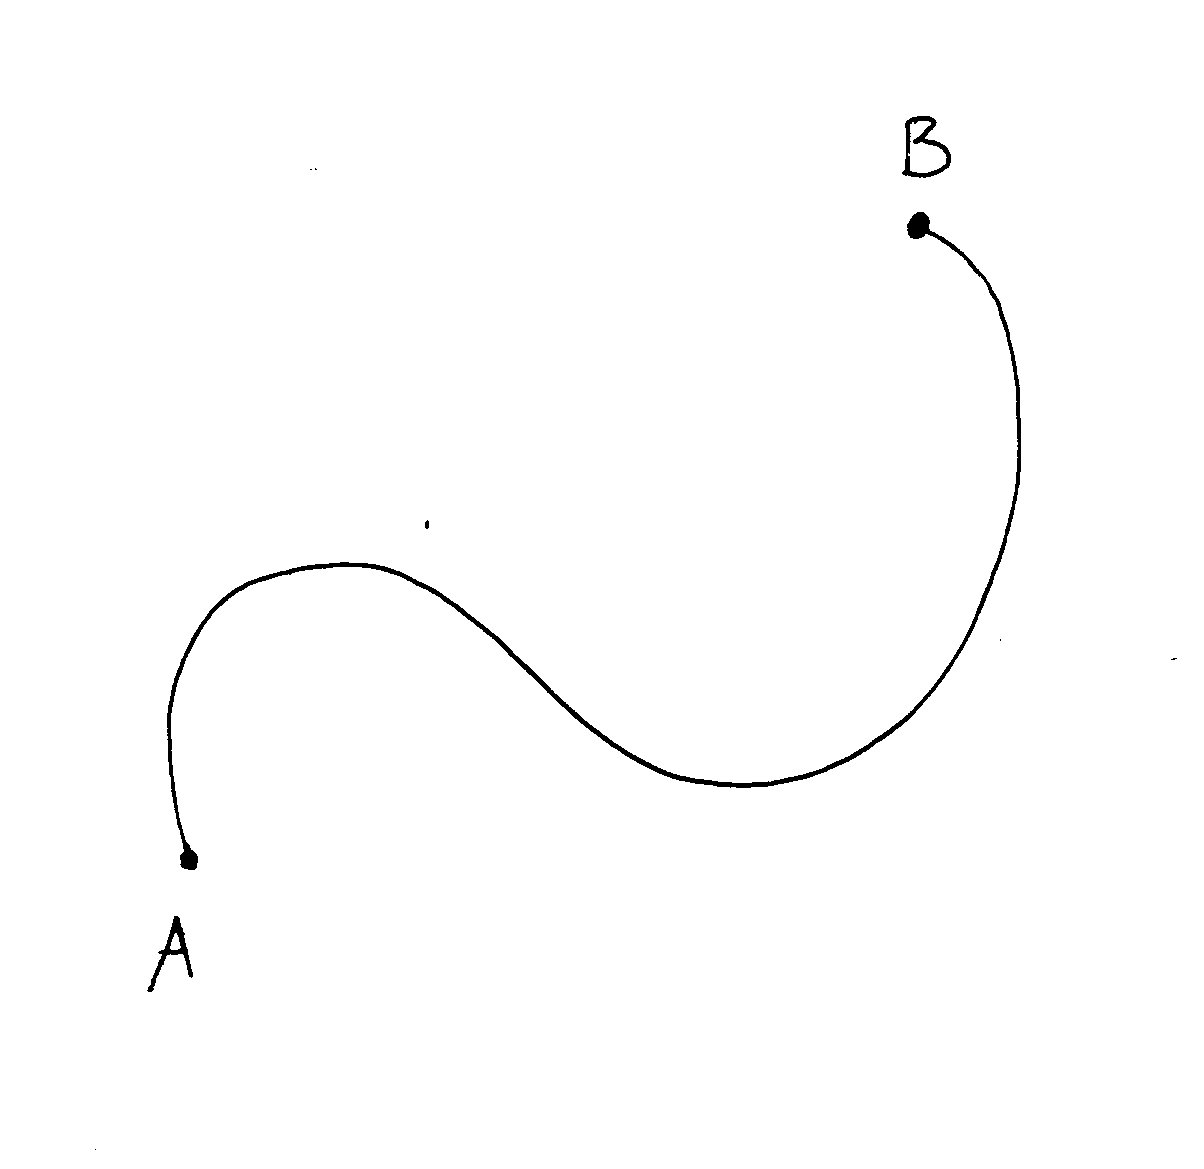
\includegraphics[width=0.4\textwidth]{image/pi_nombre/courbe1.jpg}
		\caption{Exemple de courbe comprise entre deux points $A$ et $B$.}	\label{fig_courbe}
	\end{figure} 

	Dans la première approximation de la figure \ref{fig_ligne_brisee}, une valeur approchée de la longueur $\mathscr{L}$ de la ligne comprise entre $A$ et $B$ est $AC+CD+DE+EB$. Plus la subdivision est fine, plus la ligne brisée est proche de la courbe\,: avec la ligne brisée verte, une valeur approchée de la longueur $\mathscr{L}$ serait ensuite $AF+FG+GC+CH+HI+ID+DJ+JK+KE+EL+LM+MB$. En bas, on a représenté un zoom pour montrer qu'il est toujours possible d'affiner la subdivision\,: on pourrait ajouter des points entre la subdivision de la ligne rouge.

	\begin{figure}
		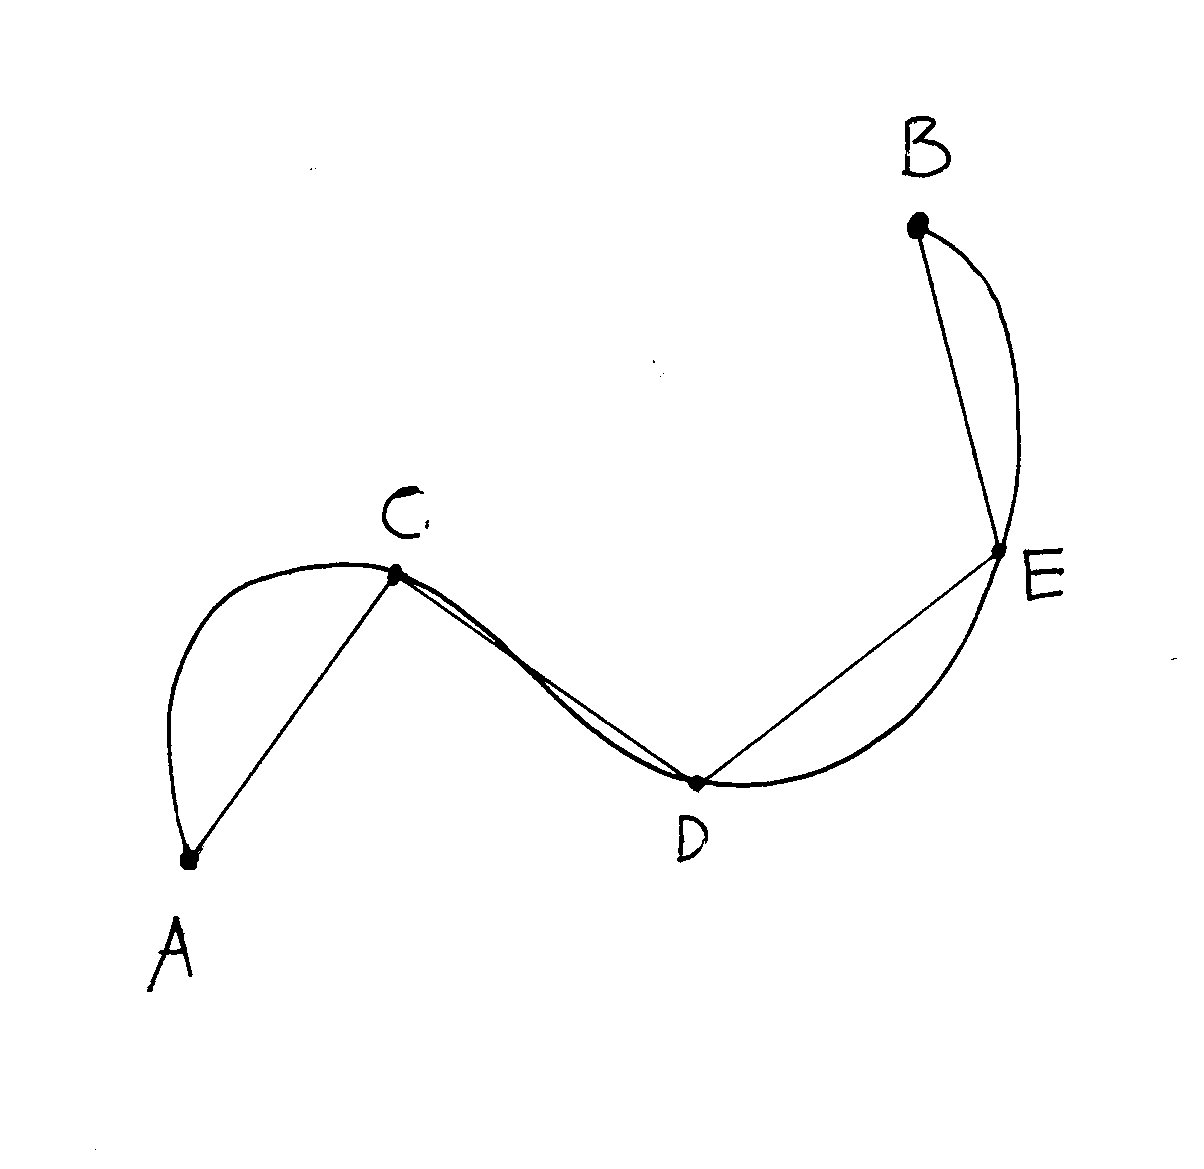
\includegraphics[width=0.45\textwidth]{image/pi_nombre/courbe2.jpg}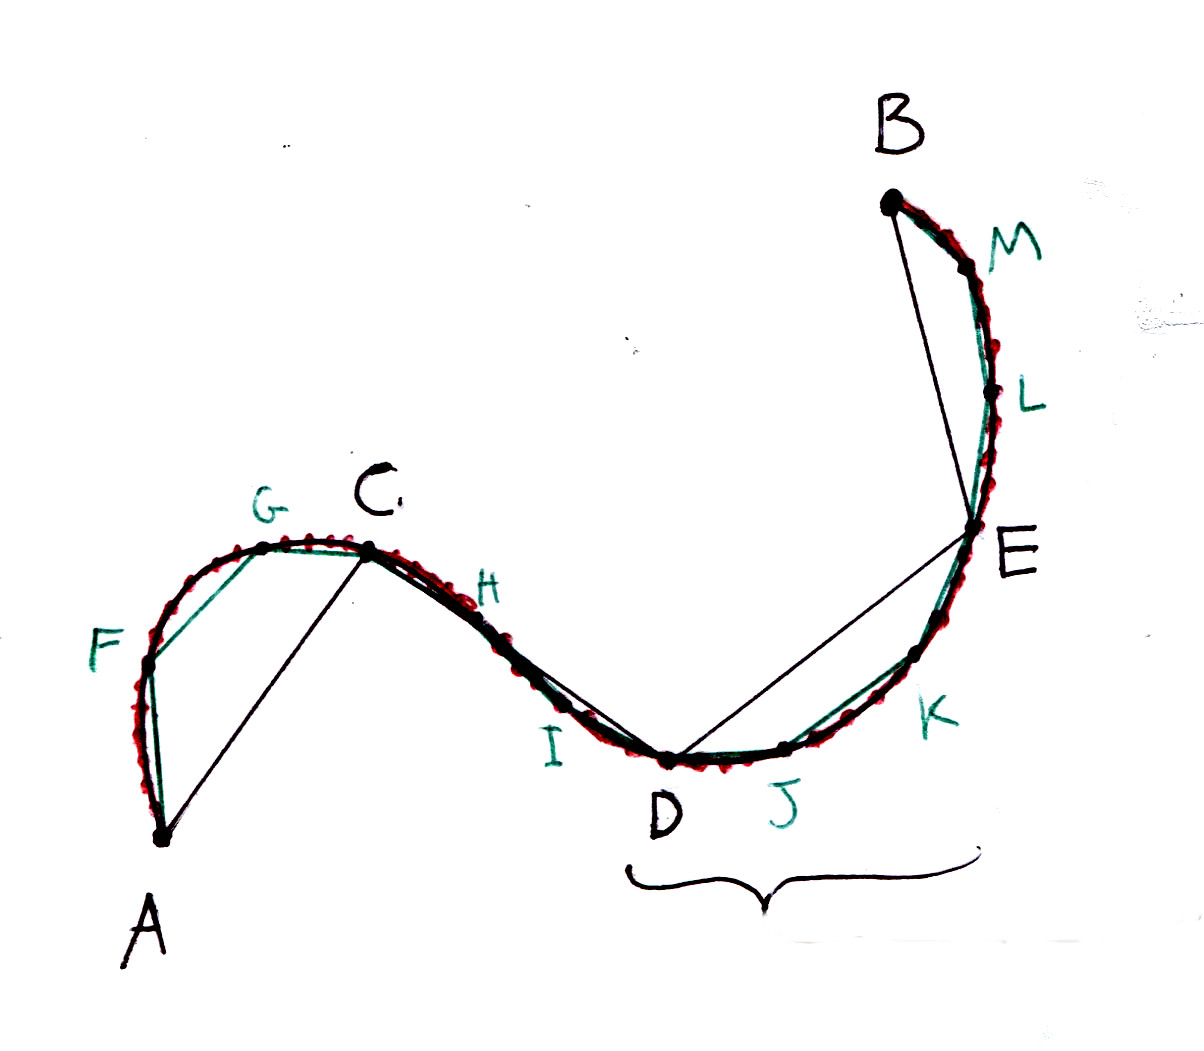
\includegraphics[width=0.45\textwidth]{image/pi_nombre/courbe3.jpg}

		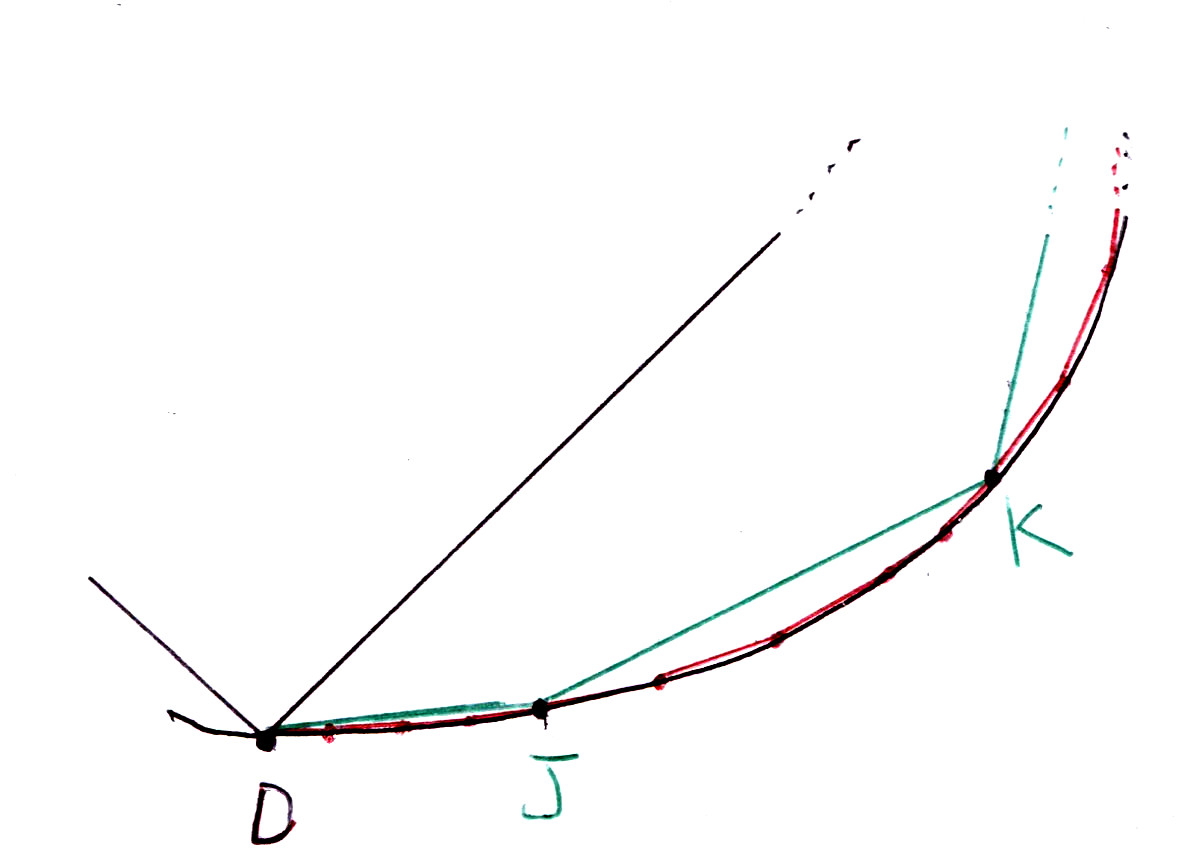
\includegraphics[width=0.5\textwidth]{image/pi_nombre/courbe4.jpg}
		
		\caption{Lignes brisées qui suivent une subdivision de plus en plus fine de la courbe comprise entre $A$ et $B$. La dernière figure représente un zoom sur celle de droite, là où on a mis une accolade.} \label{fig_ligne_brisee}
	\end{figure}

	Il faut aussi que les points de la ligne brisée soient ordonnés sur la courbe (on veut éviter les allers-retours, voir figure \ref{fig_aller_retour}). Cela fait appel à des axiomes d'ordonnancements de points le long d'un chemin. Cela se fait de la manière suivante\,: on définit une relation ternaire entre trois points : on écrira $A\star B\star C$ pour signifier que $B$ est entre $A$ et $C$ le long de la courbe. Cela peut se faire de manière axiomatique. Nous le ferons dans le chapitre \ref{chap_angle} pour les points alignés sur une droite. L'axiomatisation sur une courbe est similaire. L'extension de ces axiomes sur une courbe ne pose pas de problème en principe.

	\begin{figure}
		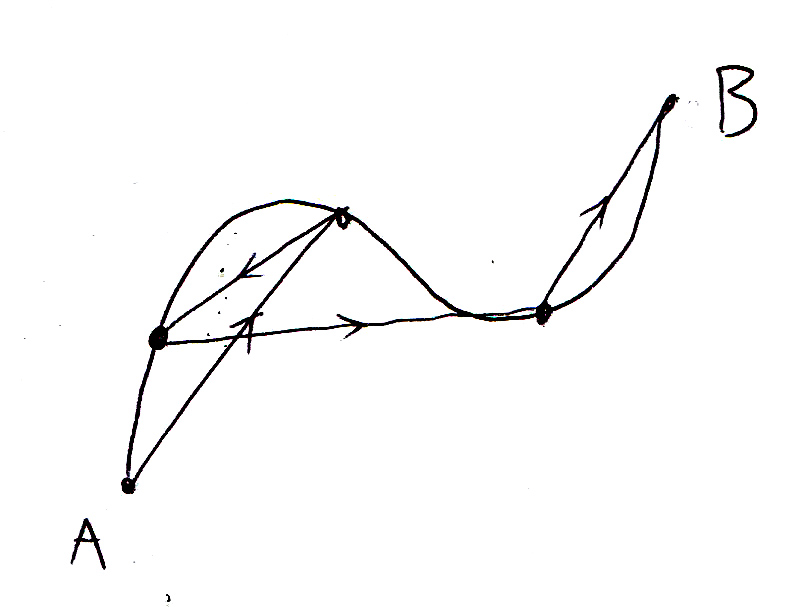
\includegraphics[width=0.4\textwidth]{image/pi_nombre/aller_retour2.jpg}
        \hfill 
        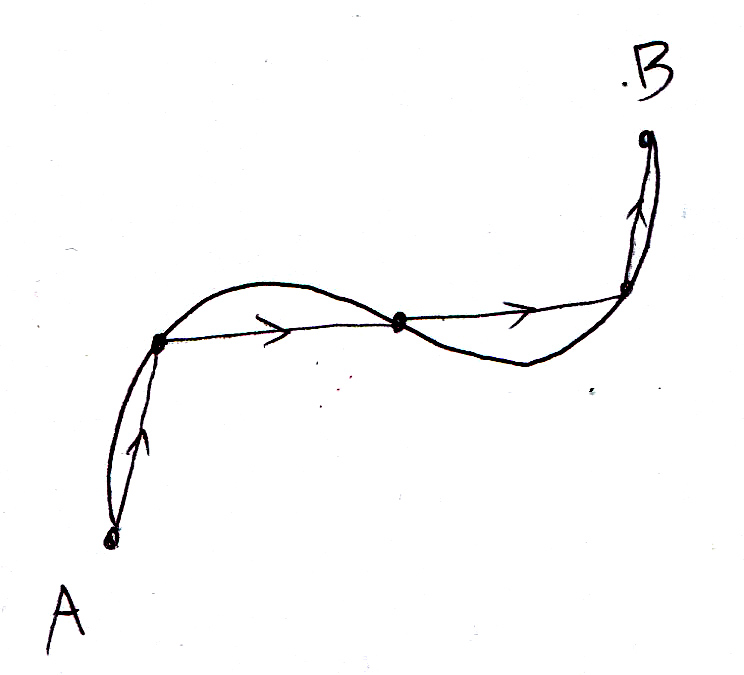
\includegraphics[width=0.4\textwidth]{image/pi_nombre/aller_retour1.jpg}
		\caption{À gauche\,: la ligne brisée fait un aller-retour. À droite\,: la ligne brisée ne fait pas d'aller-retour.}
		\label{fig_aller_retour}
	\end{figure}


	Les conditions de validité d'une telle définition ne sont pas si évidentes. D'abord, il faut s'assurer qu'il est bien possible de passer à la limite d'une subdivision infinie et qu'il est toujours possible de calculer la somme des mesures de chaque petit segment. Il existe des contres-exemples, par exemple des courbes qui occupent une aire finie mais dont le périmètre est infini\,; cela pose des problèmes dans le calcul (j'en mets un connu en annexe \ref{app_flocon}). Pour éviter les cas pathologiques, on se contentera de définir la longueur sous réserve d'existence de la limite de la longueur des lignes brisées (s'il est impossible de calculer cette limite, on décrètera que la longueur de la courbe n'est pas définie). 

	Ensuite, il faut s'assurer que lorsque l'on affine la subdivision, elle remplit bien toute la courbe\,: en effet, on pourrait ajouter une infinité de points mais seulement sur la première moitié de la courbe, et ainsi la longueur serait sous-estimée (voir figure \ref{fig_defaut_longueur}). 

	\begin{figure}
		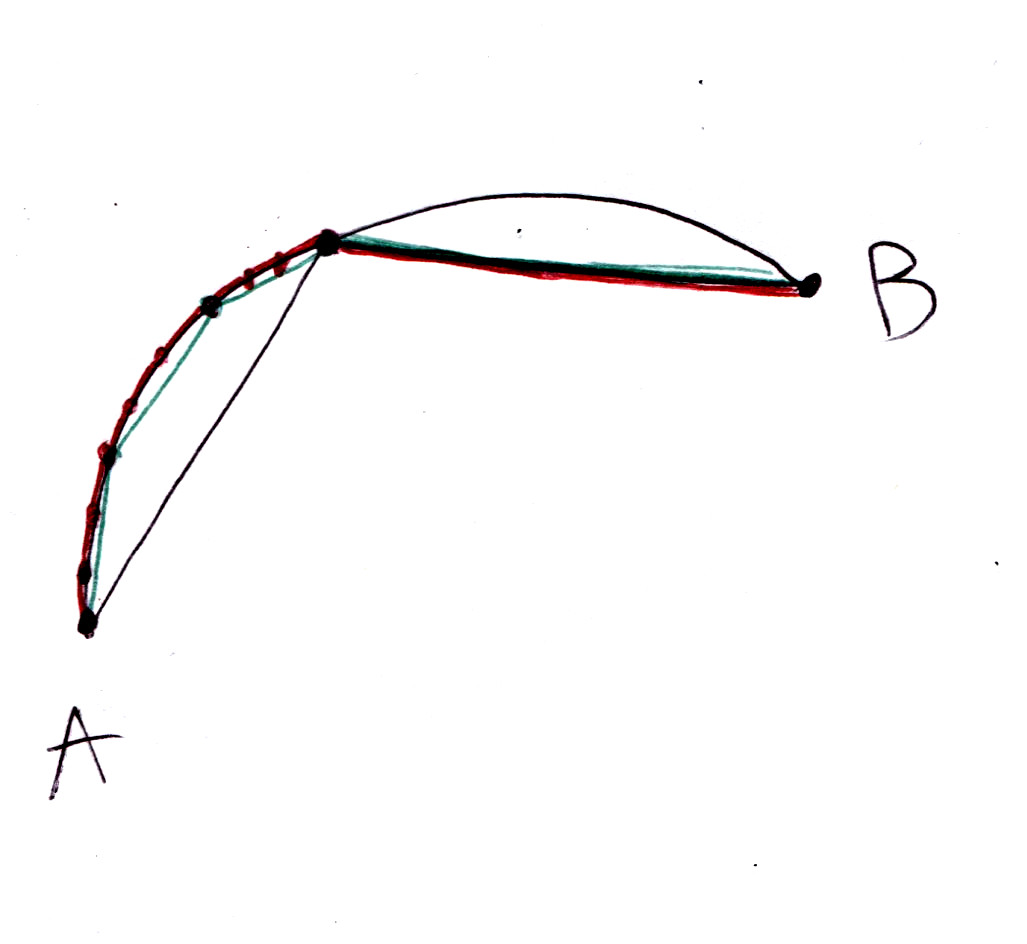
\includegraphics[width=0.4\textwidth]{image/pi_nombre/defaut_longueur.jpg}
		\caption{On approche la longueur de la courbe comprise entre $A$ et $B$ par des lignes brisées de plus en plus fines, mais on oublie de raffiner la subdivision sur toute une partie de la courbe. Ainsi, même la  mesure de la ligne brisée rouge est une mauvaise approximation de la longueur de la courbe.}\label{fig_defaut_longueur}
	\end{figure}

	Pour résoudre ce problème, on demande que la série de subdivisions de la courbe soit dense. Cela signifie que si l'on choisit un point arbitraire $M$ sur la courbe, et un rayon $r$ (strictement positif) arbitrairement petit, alors notre série de subdivision parviendra toujours à envoyer au moins un point dans la sphère de centre $M$ et de rayon $r$ (Voir figure \ref{fig_densite}). 

	\begin{figure}
		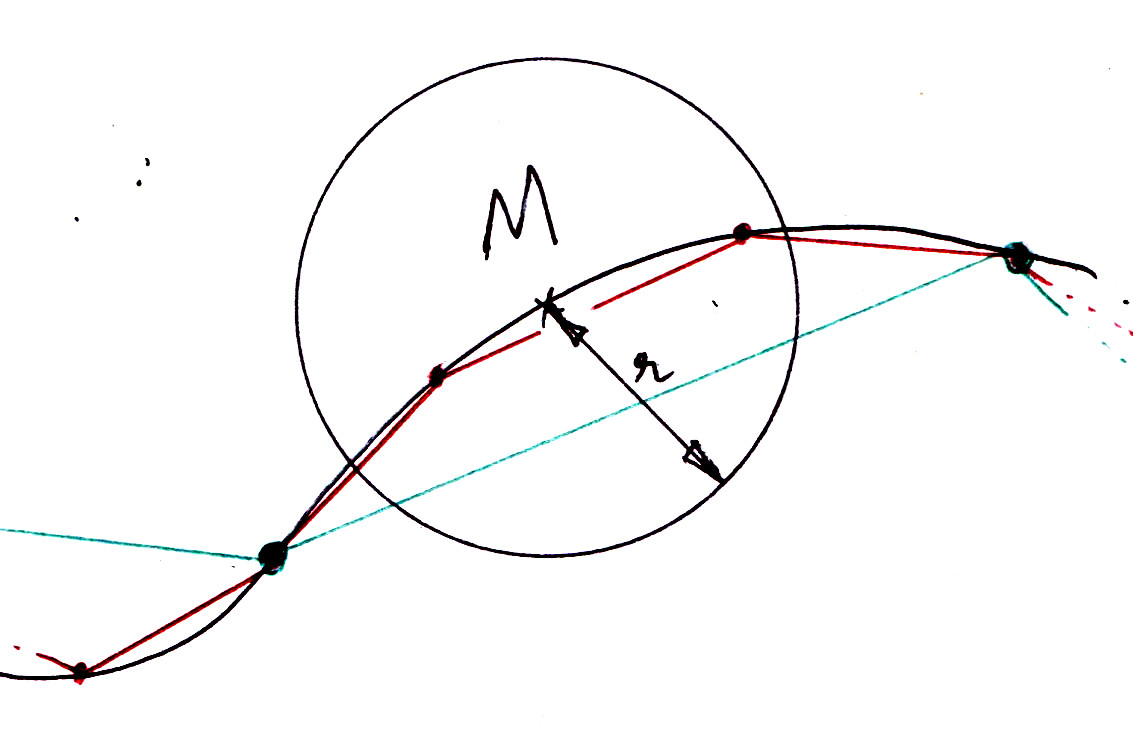
\includegraphics[width=0.5\textwidth]{image/pi_nombre/densite.jpg}
		\caption{Illustration du concept de densité. Ici, la subdivision en ligne brisée verte ne satisfait pas la condition requise, alors que la rouge oui.}\label{fig_densite}
	\end{figure}

	J'attire votre attention sur le caractère arbitrairement petit du nombre $r$. Cela signifie que si l'on prend n'importe quel point de la courbe, on pourra toujours trouver une subdivision assez fine pour qu'elle ait au moins un point aussi proche que l'on veut du point $M$. Cette propriété de densité assure que lorsque le nombre de points de la ligne brisée tend vers l'infin (ou que le rayon de la boule tend vers zéro), toute la courbe est remplie par la subdivision de la ligne brisée. Et histoire d'être sûr, il faudrait assurer que tous les points de la subdivision précédente sont contenus dans la subdivision suivante. C'est une manière de \og{}raffiner\fg\, la subdivision.

\section{Périmètre d'un cercle}

	Il est temps de commencer à approcher la longueur d'un cercle. Pour commencer nous allons considérer un cercle de rayon $R=1$. Nous allons appeler $P$ son périmètre. C'est le nombre que l'on se propose de calculer. La méthode d'Archimède a consisté à donner des encadrements de plus en plus fins de ce périmètre en encadrant géométriquement le cercle par des polygones réguliers inscrits et en inscrivant le cercle dans des polygones réguliers. Considérons une première étape constituée par une inscription d'hexagones réguliers.
	\begin{figure}
		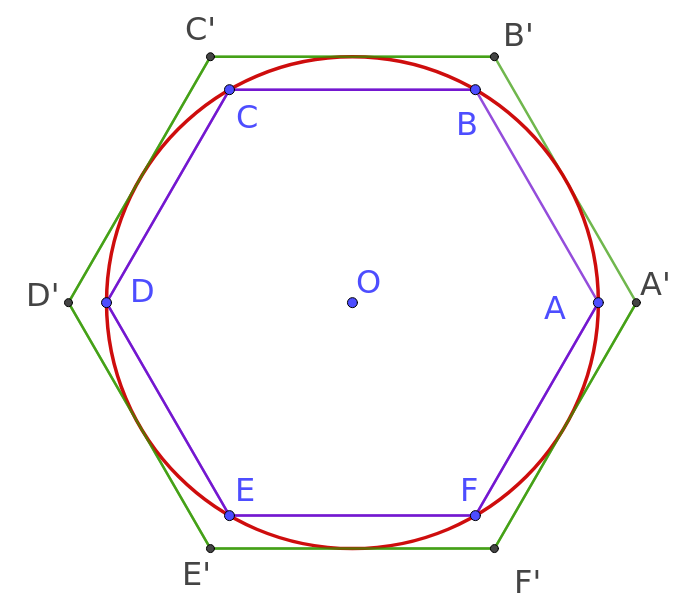
\includegraphics[width=0.5\textwidth]{image/pi_nombre/poly_inscrit.png}
		\caption{Hexagones réguliers. Le bleu est inscrit dans le cercle (chaque sommet appartient au cercle). Le vert est circonscrit au cercle (des parties du cercle touchent les côtés de cet hexagone). L'hexagone vert a ses côtés parallèles au bleu.}
	\end{figure}

	Calculons les périmètres de ces deux hexagones. Tout d'abord, on sait que $OA=1$ puisque c'est un rayon du cercle. Ensuite, joignons les sommets opposés de l'hexagone régulier. Cela forme 6 triangles isocèles dont les côtés égaux mesurent 1. Cependant, vu que l'on a partitionné un tour complet en six secteurs d'angles de mesures égales, alors chaque angle au centre mesure 360°/6=60°. Mais comme la somme des angles d'un triangle vaut 180° et que les deux autres angles sont égaux, on trouve facilement que les trois angles de chaque triangle mesurent tous 60°. Nous avons donc affaire à six triangles équilatéraux. On voulait calculer le périmètre de l'hexagone, mais en fait, chacun de ses côtés mesure le rayon du cercle, et donc, le périmètre mesure $6\times OA=6$. Ainsi, on sait que le périmètre du cercle est légèrement plus grand que 6.

	De même, on comprend facilement que le périmètre du grand hexagone mesure $6\times OA'$. Mais il nous faut calculer $OA'$.
	Considérons le triangle $OA'B'$. Traçons la médiatrice du segment $[A'B']$. Elle coupe $[A'B']$ perpendiculairement en son milieu, en $M$ et passe par $O$. Elle constitue un axe de symétrie du triangle considéré. De plus, $[OM]$ est un rayon du cercle, donc $OM=1$. Le triangle $OMA'$ est rectangle en $M$, donc d'après le théorème de Pythagore, on a
	\begin{equation}
		OA'^2=OM^2+MA'^2. \nonumber
	\end{equation}
	Mais $OM=1$ et puisque $OA'=A'B'$ et que $M$ est le milieu de $A'B'$, $MA'=\frac{OA'}{2}$. Ainsi, l'égalité de Pythagore devient
	\begin{equation}
		OA'^2=1^2+\(\frac{OA'}{2}\)^2 = 1+\frac{OA'^2}{2^2}=1+\frac{OA'^2}{4} \nonumber
	\end{equation}
	Si l'on regroupe les termes contenant $OA'$ à gauche de l'équation, on obtient
	\begin{equation}
		OA'^2+\frac{1}{4}OA'^2=1 \Leftrightarrow \(1-\frac{1}{4}\)OA'^2=1 \Leftrightarrow \frac{3}{4}OA'^2=1 \Leftrightarrow OA'^2=\frac{4}{3}.\nonumber
	\end{equation}
	On en déduit que
	\begin{equation}
		OA'=\sqrt{\frac{4}{3}}=\frac{\sqrt{4}}{\sqrt{3}}=\frac{2}{\sqrt{3}}. \nonumber
	\end{equation}
	Et enfin, le périmètre du grand hexagone mesure $6\times OA'=12/\sqrt{3}\approx6,93$.

	On obtient donc une première approximation de $\pi$\,:
	\begin{equation}
		6<2\pi<9.93 \quad\text{et donc}\quad 3<\pi<4.965\nonumber
	\end{equation}

	Cette approximation est très grossière. Que faire\,? Inspirés par la définition des longueurs des courbes dans la section précédente, divisons notre subdivision en deux, autrement dit, multiplions par deux le nombre de côtés de l'hexagone inscrit. Nous obtenons la figure \ref{fig_doubler_hex}.

	\begin{figure}
		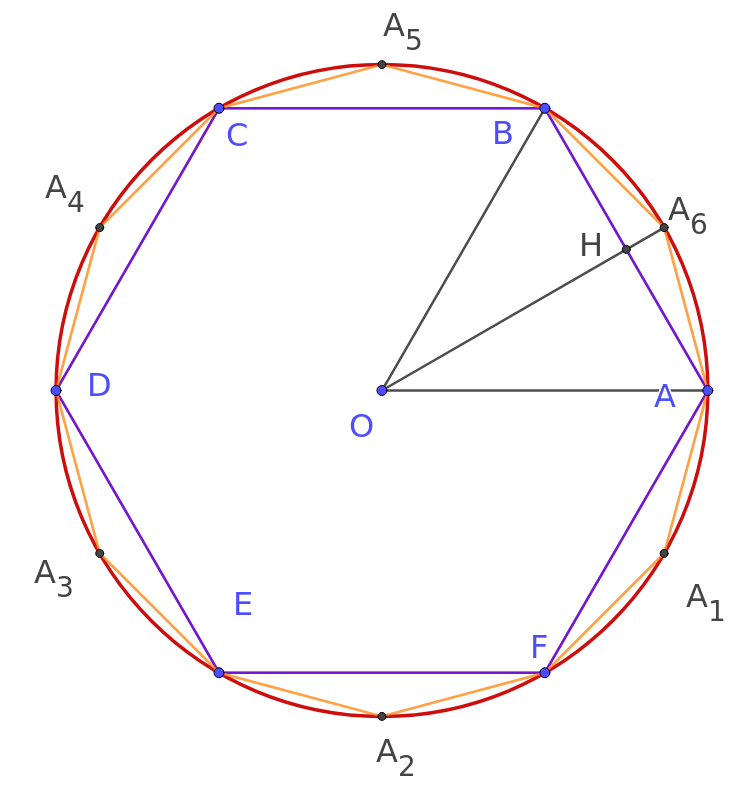
\includegraphics[width=0.6\textwidth]{image/pi_nombre/doubler_hex.png}
		\caption{Doublement du nombre de côté de l'hexagone.}\label{fig_doubler_hex}
	\end{figure}

	\noindent 3) On appelle $c_1$ la mesure du côté du dodécagone inscrit et $L_1$ son périmètre, et $d_1$ la mesure du côté du dodécagone circonscrit, et $P_1$ son périmètre. Calculer tous ces nombres. En déduire un encadrement plus fin de $\pi$.

	Supposons avoir subdivisé $n$ fois l'hexagone de départ. On aurait alors multiplié le nombre de côté par 2, $n$ fois, à savoir, par $2\times2\times2\times\ldots\times 2$ où 2 apparaît $n$ fois. Il existe une notation économique pour noter ce nombre\,: $2^n$. Au rang $n$, notons $c_n$ la mesure d'un côté de ce polygone, et notons $L_n$ la longueur de ce polygone. Puisqu'au rang $n$ il y a $6\times 2^n$ côtés, nous avons\,: $L_n=6\times 2^n c_n$. De plus, nous savons qu'au rang zéro, $c_0=1$, nous l'avons calculé plus haut.
	Pour automatiser la procédure, nous voudrions voir comment varie $c_n$ lorsque l'on passe de $n$ à $n+1$. Ensuite, un programme numérique poura aisément itérer le processus autant de fois que le permettent les ressources informatiques, étant donné le point de départ.

	Regardons comment cela se passe sur la figure \ref{fig_iter}. Supposons que le segment $[AB]$ représente le côté de longueur $c_n$. Lorsque l'on double le nombre de côtés, on construit le point $E$ à l'intermédiaire, et ainsi, $AE=EB=c_{n+1}$. Ainsi, $(OE)$ est la médiatrice du segment $[AB]$. 
	\begin{figure}
		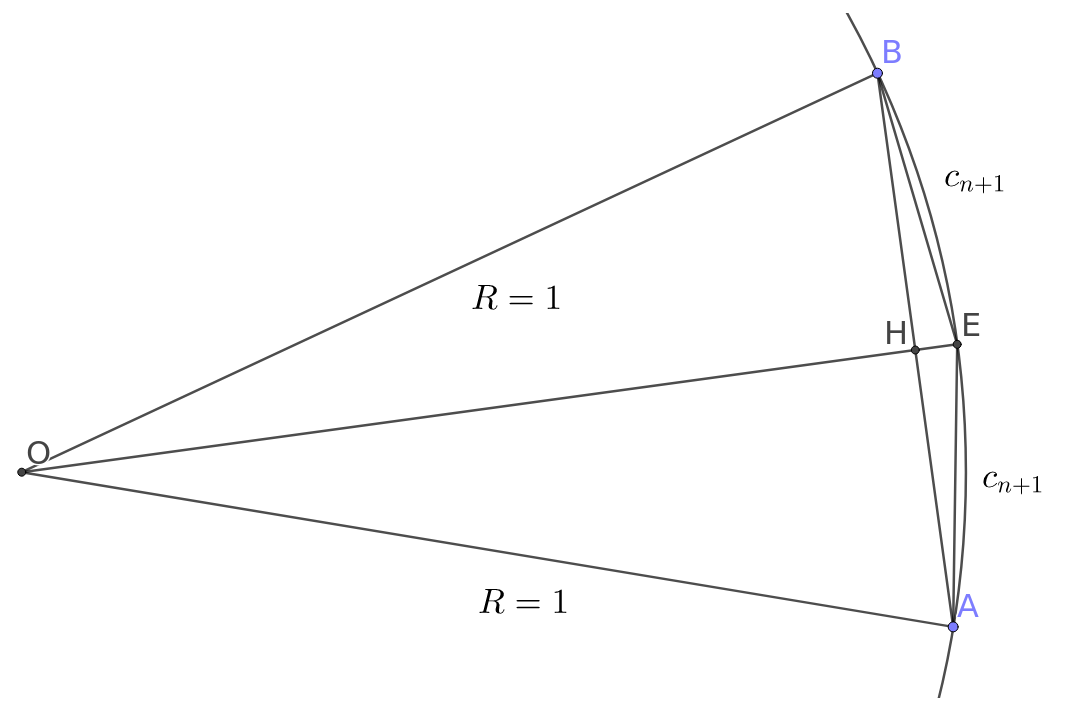
\includegraphics[width=0.6\textwidth]{image/pi_nombre/iteration.png}
		\caption{Itération pour passer du calcul de $c_n$ à celui de $c_{n+1}$.}\label{fig_iter}
	\end{figure}

	Nommons $H$ l'intersection de $(AB)$ et de $(OE)$, qui sont perpendiculaires. Dans le triangle $OAH$ rectangle en $H$, le théorème de Pythagore nous donne $OA^2=AH^2+OH^2$. Mais $OA=1$ et $AH=AB/2=c_n/2$. Après quelques manipulations, on obtient 
	\begin{equation}
		OH=\sqrt{1-\(\frac{c_n}{2}\)^2}=\sqrt{1-\frac{c_n^2}{4}}. \nonumber
	\end{equation}
	De là, on tire $HE=1-OH=1-\sqrt{1-\frac{c_n^2}{4}}$. Et enfin, dans le triangle $AHE$ rectangle en $H$,
	\begin{equation}
		c_{n+1}=AE=\sqrt{AH^2+HE^2}=\sqrt{\(\frac{c_n}{2}\)^2+\(1-\sqrt{1-\frac{c_n^2}{4}}\)^2}.\nonumber
	\end{equation}
	En développant l'identité remarquable et en simplifiant, on trouve enfin
	\begin{equation}
		c_{n+1}=\sqrt{2}\sqrt{1-\sqrt{1-\frac{c_n^2}{4}}} \label{eq_cnpu}
	\end{equation}
	Et là, on a gagné. En effet, on connaît la valeur de $c_0$ (cela mesure 1) et on sait comment passer de $c_n$ à $c_n+1$. D'ailleurs, remarquons que l'on retrouve bien le passage de $c_0$ à $c_1$ que l'on a fait un peu plus haut\,:
	\begin{equation}
		c_1=\sqrt{2}\sqrt{1-\sqrt{1-\frac{c_0^2}{4}}} = \sqrt{2-2\sqrt{1-\frac{1}{4}}}=\sqrt{2-\sqrt{3}}.\nonumber
	\end{equation}

	\usemintedstyle{bw}

	Dans un simple tableur, voici comment il suffirait de procéder pour approcher la valeur de $\pi$ (voir figure \ref{fig_approx_pi}).
	Dans la colonne $A$, on représente le nombre d'itérations $n$. Dans la colonne $B$, on représente le nombre $2^n$. Pour ce faire, il suffit d'écrire la formule \mintinline{python}{=2^A2} dans la case B2, puis d'étendre la formule sur toute la colonne. Cela donne un ordre de grandeur du nombre de côtés. Ensuite, il faut s'occuper de la colonne des côtés. On commence par itérer la valeur 1 dans la case $C2$. Ensuite, dans la case $C3$, on rentre la formule suivante\,: \mintinline{python}{=RACINE(2)*RACINE(1-RACINE(1-C2*C2/4))}. Puis on étend. Enfin, on s'occupe de la colonne des longueurs. Dans la colonne des longueurs, on rentre simplement, en case $D2$, la formule \mintinline{python}{=6*B2*C2}. Puis on étend. Et pour obtenir une approximation du nombre $\pi$, on divise par deux (dernière colonne).
	\begin{figure}
		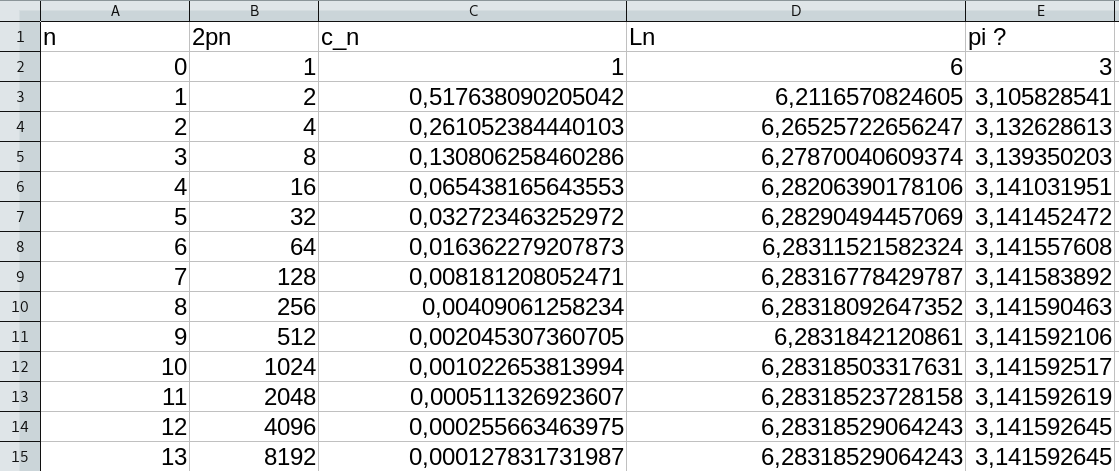
\includegraphics[width=\textwidth]{image/pi_nombre/approx_pi.png}
		\caption{Approximation de $\pi$ avec un tableur.}\label{fig_approx_pi}
	\end{figure}


	Pour être véritablement complet, il faudrait aussi faire de même avec le polygone circonscrit au cercle. Nous laissons cela en exercice au lecteur\,!

	\paragraph{Exercice} On considère l'hexagone circonscrit au cercle de rayon 1. De même, on va multiplier par deux le nombre de ses côtés de telle sorte que chaque côté soit tangent au cercle, et qu'à chaque itération, le polygone est régulier. Démontrer que si l'on note $d_n$ la mesure du côté du polygone circonscrit au cercle, et $P_n$ son périmètre, alors on a
	\begin{align}
		d_0&=\frac{2}{\sqrt{3}} \\
		P_0&=\frac{12}{\sqrt{3}} \\
		d_{n+1}&=\sqrt{2}\sqrt{\sqrt{\frac{d_n^2}{4}+1}-1} \label{eq_dnpu}\\
		P_n&=6\times 2^n d_n.
	\end{align}

\section{Conclusion\,: $\pi$ est-il vraiment un nombre\,?}
	Il nous reste une dernière chose à démontrer\,: que le nombre $\pi$ ainsi calculé ne dépend pas du rayon du cercle. En effet, jusqu'ici nous n'avons calculé que le périmètre d'un cercle de rayon 1, et nous avons divisé par son diamètre particulier ($D=2R=2$) pour obtenir une approximation de $\pi$. Qu'obtiendrions-nous si nous faisons le même processus sur n'importe quel cercle\,?

	C'est le théorème de Thalès qui nous permet de vérifier que le nombre $\pi$ est invariant par modification du cercle.

	\begin{figure}
		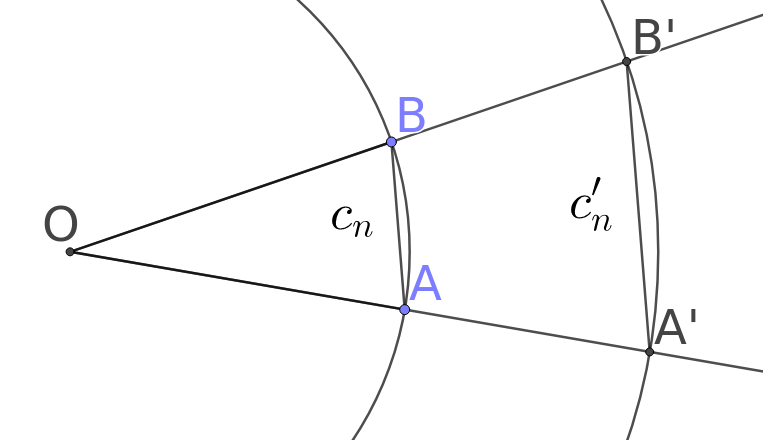
\includegraphics[width=0.6\textwidth]{image/pi_nombre/thales.png}
		\caption{Illustration d'une étape du calcul du périmètre des deux cercles emboîtés.}\label{fig_semblabilite}
	\end{figure}


	Considérons deux cercles de rayons différents et procédons de même pour approcher leur périmètre\,: on subdivise les cercles en des polygones réguliers inscrits. Déplaçons les figures de telle sorte que les deux centres des deux cercles coïncident, et qu'à l'étape $n$, les demi-droites formées par les centres des cercles et les sommets des polygones coïncident. C'est toujours possible, car au rang $n$, l'angle formé par les deux sommets les plus proches du polygone et le centre sont identiques (on divise un tour complet en $6\times 2^n$ secteurs d'angles égaux de même mesure). Nommons $c_n$ le côté du polygone inscrit du petit cercle, et $c_n'$ le côté du polygone inscrit du grand cercle (voir figure \ref{fig_semblabilite}). Les deux triangles $OAB$ et $OA'B'$ sont semblables. En effet, ils sont isocèles, et partagent un angle (au centre du cercle). Ainsi, $\widehat{OAB}=\widehat{OA'B'}=\widehat{OBA}=\widehat{OB'A'}$. Par propriété des angles alternes-internes, $(AB)\sslash(A'B')$. On peut donc utiliser le théorème de Thalès\,:
	\begin{equation}
		\frac{OA}{OA'}=\frac{AB}{A'B'}. \nonumber	
	\end{equation}
	En notant $R=OA$ et $R'=OA'$, on obtient alors
	\begin{equation}
		\frac{R}{R'}=\frac{c_n}{c_n'}\quad\text{donc}\quad \frac{c_n}{R}=\frac{c_n'}{R'}. \nonumber
	\end{equation}
	Au rang zéro, le périmètre de l'hexagone du petit cercle mesure $L_0=6R$ et celui du grand, $L_0'=6R'$. Au rang $n$, on a tout simplement $L_n=6\times 2^n c_n $ et $L_n'=6\times 2^n c_n' $.
	La valeur approchée au rang $n$ de $\pi$ pour le petit cercle vaut donc\,:
	\begin{equation}
		\pi_n=\frac{1}{2R}6\times 2^n c_n = 3\times 2^n \frac{c_n}{R}.\nonumber
	\end{equation}
	Mais comme $c_n/R=c_n'/R'$, en fait, $\pi_n=\pi_n'$. 

	On vient de démontrer que le calcul de $\pi$ ne dépend pas de la taille du cercle considéré, et donc, on peut raisonnablement poser\,:
	\begin{equation}
		\pi=\lim\limits_{n\to\infty}\pi_n \nonumber
	\end{equation}

	{\bfseries Et donc $\pi$ est bien un nombre. CQFD\,!!!}

	Remarque : il reste une arnaque dans la démonstration. À aucun moment nous n'avons démontré que les suites de nombres $(L_n)$ et $(P_n)$ convergeaient bien vers un nombre, et encore moins que c'était le même nombre. Un constat empirique ne vaut pas une démonstration mathématique. Nous la reportons en annexe \ref{app_conv}. 

\section{Flash forward\,: calculer $\pi$ à l'aide des fonctions trigonométriques}

	Considérons un cercle trigonométrique dans lequel on inscrit un polygone régulier à $n$ sommets. Alors l'angle au centre formé par deux sommets consécutifs mesure $2\pi/n$. Un simple calcul de trigonométrie permet de vérifier que la distance qui sépare deux sommets consécutifs mesure $2\sin(\pi/n)$. Le périmètre d'un tel polygone mesure alors $P_n=2n\sin(\pi/n)$ et donc on peut prouver que
	\begin{equation}
		\pi=\lim\limits_{n\to\infty}n\sin\(\frac{\pi}{n}\).\label{eq_serpent}
	\end{equation}
	Mais à ce stade, c'est un peu le serpent qui se mord la queue...


\newpage
    

\chapter{Qu'est ce qu'un angle\,?}
\label{chap_angle}

%\initial{L}{'angle} est comme tout ce qui semble évident, plutôt laborieux à définir. Dans son acception ancienne l'angle représente une portion de plan entre deux demi-droite, le secteur d'angle, alors qu'aujourd'hui elle se confond souvent avec la mesure de l'angle. Ces représentations ne sont pas fondamentalement en désaccord une fois déployé l'ensemble les distinctions et relations qui les lient. 

%\remarquehistoireimage{On sait peu de chose de la vie d'Euclide sinon qu'il aurai vécu autour du \Romanbar{3}\iemes siècle avant notre ére. Son ouvrage : \href{http://promenadesmaths.free.fr/telecharger/euclide_elements_1804.pdf}{Éléments} contient une tentative quasiment aboutit de construction d'une géométrie axiomatique. Il contient de nombreux théorème et leurs démonstrations. Il connue de nombreuses éditions et les copies successives contiennent des ajouts ou modifications de ceux qui les produire de sorte que le texte qui nous est parvenue n'est pas tout a fait le texte produit par Euclide. On peut néanmoins supposer que ces modifications respectent l'esprit d'Euclide. Son contenue reste au centre de l'enseignement de la géométrie du secondaire.}{image/EuclideGravure.jpg}

%Une tentative de construction des ces axiomes fut pour la première fois établis par Euclide dans ses \href{http://promenadesmaths.free.fr/telecharger/euclide_elements_1804.pdf}{Éléments}. En 1899, les << \'Eléments >> d'Euclide ne satisfont plus les mathématiciens. Non pour ses éventuelles limitations, mais parce que justement le système d'axiome proposé par Euclide est lacunaire. Plusieurs fois, dans la lecture des \emph{éléments}, on remarque que certains résultats, implicitement considérés comme vrai, sont utilisés sans avoir fait l'objet de démonstrations. Et pour cause, avec les axiomes présents, ils sont indémontrable. Le but de la relecture par Hilbert est de proposer un système d'Axiome suffisant, respectant l'esprit de la construction Euclidienne et permettant d'aboutir à la même géométrie. Il publiera les résultats de ses travaux dans un livre : <<\href{https://www.pedagogie.ac-aix-marseille.fr/upload/docs/application/pdf/2019-11/principes_fondamentaux_geometrie_-_david_hilbert.pdf}{Les principes fondamentaux de la géométrie}>> qui sera traduit et publié en français en 1900. C'est dans l'esprit axiomatique de Hilbert que nous présenterons dans cette sections 

%\remarquemargehistoireimage{David Hilbert (1862-1942) est un mathématicien Allemand ayant travaillé principalement a l'université de Göttingen. Il est connue pour sa ré-axiomatisation de la géométrie d'Euclide mais aussi ses traveaux autour des espace di de Hilbert, \cad des espaces vectoriels (réels où complexe) sur lequel est définie un produit scalaire et complet pour la distance issue du produit scalaire. Il vivra très difficilement l'exclusion de ses collègue juifs loirs de la période nazi et lorsque la ministre nazi lui demandera : \og Comment se trouvent les mathématiques à Göttingen maintenant qu'elle est libre de l'influence juive ? \fg Hilbert répliquera : \og Des mathématiques à Göttingen ? Il n'y en a plus guère \fg. Sur sa tombe est gravé \og Wir müssen wissen, wir werden wissen \fg : soit \og Nous devons savoir, nous saurons\fg. }{image/Hilbert.jpg}{15cm}

    %\section{Notion première}\label{subsec-notionpremiere}
    
    %\section{Pourquoi reprendre aux niveaux des axiomes?}
\begin{quote}
    Le bien connu en général, pour la raison qu'il est bien connu, n'est pas connu. C'est la façon la plus commune de se tromper et de tromper les autres, à propos du connaître, que de présupposer quelque chose comme bien connu.

    Georg Wilhelm Friedrich Hegel, \emph{Phénoménologie de l’esprit.}
\end{quote}
%\epigraph{Le bien connu en général, pour la raison qu'il est bien connu, n'est pas connu. C'est la façon la plus commune de se tromper et de tromper les autres, à propos du connaître, que de présupposer quelque chose comme bien connu.}{Georg Wilhelm Friedrich Hegel, Phénoménologie de l’esprit}

%\addlb{Commentaire général\,: tu pars beaucoup trop dans tous les sens en évoquant plein de notions avancées qui ne sont pas abordées dans le texte (ex : séries entières). Donc la majorité de ton intro est hors sujet et illisible. Seul le dernier paragraphe, dans lequel tu annonces l'objectif du chapitre, est vraiment pertinent. Ton introduction historique suppose déjà une connaissance assez solide des mathématiques, et est donc illisible pour notre public. Il faut quasiment tout récrire.}

\initial{S}{i} la construction axiomatique de la géométrie a été pour la première fois portée par Euclide, la liste d'axiomes qu'il propose est incomplète. Certains résultats, implicitement considérés comme vrai, sont utilisés sans avoir fait l'objet de démonstrations. Et pour cause, avec les axiomes présents, ils sont indémontrable. On se placera par conséquent d'avantage dans la formulation faite par Hilbert \cite{HilbertLesPF}. 
% \guil{\href{https://www.pedagogie.ac-aix-marseille.fr/upload/docs/application/pdf/2019-11/principes_fondamentaux_geometrie_-_david_hilbert.pdf}{Les principes fondamentaux de la géométrie}}. 

%qu'on peut qualifier d'axiomatique synthétique.

Les axiomatiques d'Euclide et de Hilbert ont ceci en commun qu'elles s'appuient toutes deux sur les notions premières de points, de droite, de plan, d'appartenance, d'union et d'intersection. On parle d'axiomatique synthétique. Cette notion d'axiomatique synthétique où de géométrie synthétique est apparue au cours du \Rom{19} $^\e$ siècle par opposition a la géométrie analytique, celle qui repose sur les nombres, le calculs. Dans la pratique vraiment concrète des mathématiques cette opposition est une précieuse ridicule typique des querelles de mathématiciens. Jean Dieudonné qualifiera cette opposition de \guil{grotesques querelles des géomètres "synthétiques" et des géomètres "analytiques", aussi incompréhensibles pour nous que les discussions byzantines sur le sexe des anges, ont rempli des volumes au XIX$^\e$ siècle}. Euclide \cite{euclidelements} ne s'embarrasse pas d'une telle opposition\,: dès les axiomes de ses \guil{\href{http://promenadesmaths.free.fr/telecharger/euclide_elements_1804.pdf}{éléments}}, sa construction de la géométrie mélange axiomes synthétiques et axiomes analytiques. Néanmoins à mesure que se développe l'exposé de résultats majoritairement synthétiques (par exemple nombre de points dans l'intersection de deux droites), on passe à une majorité de résultats qu'on pourrait qualifier d'analytiques (Théorème de l'angle extérieur, Thalès ou encore Pythagore). Bref, à mesure que se déploie la géométrie chez Euclide ou même à travers l'histoire, les mathématiciens partent d'objets géométriques (synthétiques) pour en déduire des propriétés analytiques qui leurs sont attachées (Al-Kashii, volume du cône, surface sous la parabole, volume d'une sphère). Les résultats analytiques furent si nombreux que dès Pythagore, nombreux sont ceux qui pensèrent que \guil{tout est nombre}. Ce n'est cependant qu'après assimilation de la notion de repère Cartésien (présenté par Descartes dans \guil{\href{http://www.ffn.ub.es/luisnavarro/nuevo_maletin/Descartes\%20(1637)_Geometrie.pdf}{La géométrie, livre premier}} \cite{descartesgeometrie} \footnote{Disponible ici \url{http://www.ffn.ub.es/luisnavarro/nuevo_maletin/Descartes\%20(1637)_Geometrie.pdf}}) qu'on pouvait, sans nul doute, penser pouvoir reconstruire la géométrie uniquement à partir des nombres. Or la constructions axiomatique des nombres en particulier, les nombres réels, devra attendre 1869 (Meray, Cantor) et Dedekind (1872). Cette difficulté dans l'axiomatisation des nombres réels est une des cause du caractère parfois hasardeux de certaine démonstration d'Euclide. Sans nombres réels la notion de distance est susceptible d'être conçue de façon bancale. 



La reconstruction de la géométrie par les nombres et à partir des nombres uniquement (géométrie affine ou analytique) à travers la notion d'espace vectoriel, puis d'espace vectoriel euclidien (par Hilbert également) va permettre un vaste déploiement de nouveaux résultats. Elle va permettre de formaliser toute une gamme de géométrie non-euclidienne (variété topologique, différentiable, Riemannienne). Ces géométries d'abords découvertes à travers la tentative infructueuse de démontrer le cinquième axiome d'Euclide, l'axiome des parallèles, devait, si l'ont voulait les construire avec une axiomatique synthétique, utiliser chacune sa liste d'axiomes. Ce qui est long, et laborieux. Au \Rom{19}$^\e$ siècle, le souffle de la devise Pythagoricienne semblait irrésistible et c'est la raison de la réaction fondant le courant de géométrie synthétique. 
\FigureMarge{Solutions du problème d'Appolonius.}{1.2}{image/Appolonius.png}
L'approche synthétique était justifiée pour des problème comme le problème d'Appolonius (chercher les cercles tangents à trois cercles donnés dans le plan, voir figure ci contre) dont la résolution par une approche analytique est longue et ardue alors que sa résolution synthétique est courte et élégante. Dans tout les cas, avant cette formalisations affine des géomètries non-euclidienne, les mathématiciens travaillent dans certaines d'entre elle (Sphère, Lobatchevkii, disque de Poincarré) classées souvent en deux ensembles (Hyperbolique ou Elliptique) suivant la façon qu'elle ont de nier l'axiome des parallèles. Ces géométries suivent donc une axiomatique dans l'esprit d'Euclide, a mi chemin entre une approche synthétique et une approche analytique. L'exigence démonstrative a monté en gamme depuis Euclide et c'est dans dans cette approche que Hilbert va chercher a refonder une axiomatique engendrant la géomètrie d'Euclide. Cette exigence de rigueur va le pousser à adopter une axiomatique purement synthétique, remplaçant les notions de longueur ou de mesure d'angle par la notion de congruence (qu'il axiomatisera). Au bout d'un certains déploiement, et en y adjoignant l'axiomatique des nombres, ces notions de longueurs et de mesure d'angles sont reconstructibles ainsi que toute la géométrie d'Euclide. 





Le but du présent chapitre est de déployer entièrement la notion d'angle et de mesure d'angle. Dans son acception ancienne l'angle représente une portion de plan entre deux demi-droites, le secteur d'angle, alors qu'aujourd'hui elle se confond souvent avec la mesure de l'angle. Ces représentations ne sont pas fondamentalement en désaccord une fois déployé l'ensemble les distinctions et relations qui les lient. Mais alors pourquoi partir de l'axiomatique de Hilbert\,? Pourquoi réexploiter cet attirail dans un cours comme celui-ci\,? Pourquoi ne pas faire une approche affine (espace vectoriel euclidien)\,? Ou une approche semi-intuitive, semi-synthétique, semi-analytique à la Euclide\,?  À la première question de l'emploi de la géométrie fondée sur les espaces vectoriel, nous répondrons que cette approche est plus calculatoire, aspect des mathématiques que nous avons déjà vastement exploré dans les autres parties de ce cours. La principale raison est que cette approche nécessiterait une autre artillerie moins immédiatement géométrique pour être déployé. Une autre raison est que nous souhaitons, dans cette partie, familiariser le lecteur avec une mathématiques plus déductive, plus éloigné du nombre est du calcul et se concentrer nos effort sur la déduction et la démonstration. Enfin nous souhaitons faire apparaître la notion de cosinus et de sinus à partir de l'angle et donc de la figure, non à partir du calculs comme cela se ferait dans l'approche affine. À la seconde question de l'emploi de l'approche Euclidienne, certaines de ces démonstrations, a travers les résultats implicites non démontré, et \emph{non démontrable}, permettent d'appréhender mais pas de comprendre ce qu'est une preuve. L'approche de Hilbert, si son emploi dans toutes les partie du cours visant à obtenir des résultats et des formules utilisables par d'autre science est inutile, elle peut permettre, je le pense, d'acquérir l'esprit de la preuve en mathématique. Sur quelque chose qu'on pense bien connue : l'angle en géométrie. Qu'est ce qu'un angle\,? Dans l'esprit de la maxime de Hegel introduisant le chapitre 6\,: nous souhaitons montrer à quel point ce qui est conçu comme évident (içi l'angle) nécessite pour être conçu concrètement (\cad dans toutes ses déterminations) un travaille long et laborieux. L'axiomatique de Hilbert nous permettra d'atteindre ce but. 

%\citeauthor{descartesgeometrie}

%\addlb{[Tu ne reponds pas `a cette question ! D’autant plus que c’est l’approche que j’ai l’habitude d’utiliser lorsque je donne cours `a des debutants en maths.]LB }

%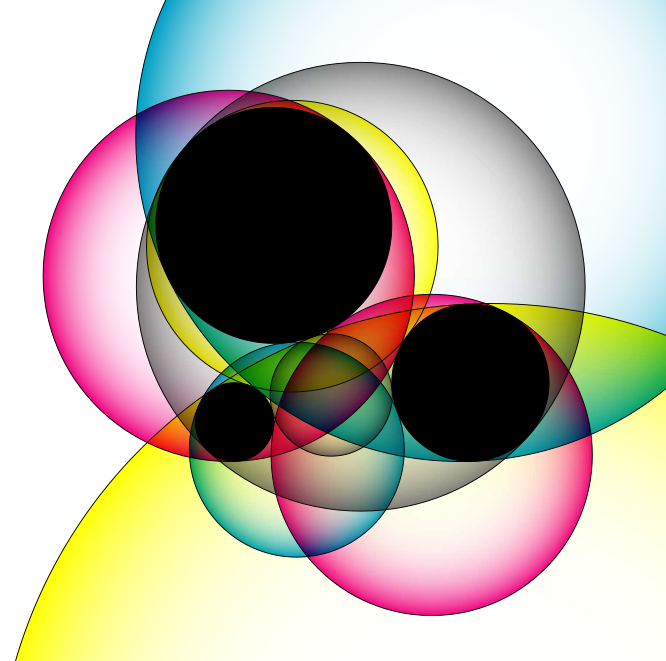
\includegraphics[width=4cm]{image/Appolonius.png}

        \section{Axiomes et notations}

%\addlb{[Peut-on supprimer l'espace entre "premières" et le point juste au dessus ?]} 

\begin{notion}
La construction axiomatique synthétique (à partir des points, des droites etc.) du plan euclidien consiste en ceci\,: on admet l'existence d'un ensemble appelé plan euclidien (qu'on notera $\mathcal{E}$), dont les éléments sont appelés points. On admet également l'existence d'un ensemble de sous-parties appelées droites (noté $\mathfrak{P}$). Le plan euclidien contient au moins une droite. 
\end{notion}

Les droites seront définies à travers les relations qu'elles entretiennent avec les points (axiomes d'incidence). Sur ces droites sont définies une notion d'ordonnancement à trois points caractérisée par les axiomes d'ordre, complétés par un axiome fort utile quand les points ne sont plus alignés : l'axiome de Pasch. Hilbert poursuit sa construction avec les axiomes dits de congruence concernant les règle de la relation du même nom. La congruence sous-tend, de façon synthétique, les notions de longueur et de mesure d'angle. Enfin, Hilbert introduit les axiomes de continuité qui vont caractériser les relations qu'entretiennent entre eux les points d'une droite quelquonque. Enfin l'axiome des parallèles est nécessaire afin de contraindre la géométrie a être Euclidienne. 

%Dans la suite on supposera connue la notion de longueur et nous construiront les notions d'angle et de mesure d'angle indépendamment des axiomes de congruence. 

 %On supposera connue la notions de distance entre points et rappellerons ceux des postulats d'Hilbert nécessaire à notre construction.

Dans la suite on notera les points (éléments de $\mathcal{E}$) en lettre latine majuscule ($A,B,C...$), les droites en lettre latine parenthésé minuscule ($(d),(e),(f)...$). 

%Ces axiomes peuvent se regrouper en cinq groupe. Le premier regroupes les axiomes d'incidences et décrit les relations d'appartenance entre points, droite et plan. Les axiomes d'ordres permettent de définir la relations "etre entre" et permettent de construire les notions de segment de demi-droit et de demi-plan. Les axiomes de congruences definissent la relations dites de congruences permettant de 

        \subsection{Axiomes d'incidences}\setcounter{serieaxiom}{1}\setcounter{axi}{0}

%\FigureMarge{Axiomes \ref{axi-A1} et \ref{axi-A2}}{image/axiome_d1.png}

%\marginnote{%
%    \tikzpicture[]
%        \node[text width=\marginparwidth, font=\small, align=center] (box) {Axiomes \ref{axi-A1} et \ref{axi-A2} \\ 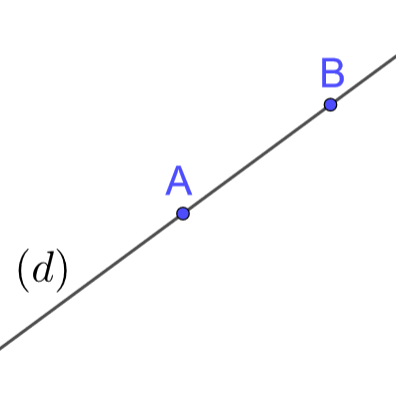
\includegraphics[width=0.7\marginparwidth]{image/axiome_d1.png}};
%\endtikzpicture
%}[0.0cm]

Hilbert commence par demander comme Euclide à ce qu'il ne passe qu'une droite entre deux points :
\FigureMarge{Axiomes \ref{axi-A1} et \ref{axi-A2}}{1.2}{image/axiome_d1.png}

\begin{axi}\label{axi-A1}
Soient $A$ et $B$ deux points distinct, il existe une unique droite $(d)$ contenant $A$ et $B$. On note $(AB)$ cette unique droite.  
    \begin{equation*}
        \forall A, B \in \mathcal{E},\, A,B \text{ distincts },\exists!(d), A,B\in(d)\,.
    \end{equation*}
\end{axi}
\begin{rema}
    De l'axiome \ref{axi-A1} on déduit que $(AB)=(BA)$. On déduit également que si $C$, distinct de $A$ et $B$, appartient également à $(d)$ alors $(d)=(AC)=(BC)=(AB)$. 
\end{rema}
L'axiome qui suit (Ax. \ref{axi-A2}) assure alors que toute droite contient au moins deux points sur une droite donnée. Ce genre de questionnement d'existence n'apparaît pas chez Euclide et y est supposé évident.
\begin{axi}\label{axi-A2}
    Soit une droite $(d)$, alors il existe au moins deux points sur cette droite.
    \begin{equation*}
        (d)\in\mathcal{D} \Rightarrow \exists A,B\in (d)\,.
    \end{equation*}
\end{axi}
De même l'axiome (Ax.\ref{axi-A3}), qui suit assure l'existence de points cette fois-ci en dehors d'une droite donnée. Cet axiome assure en quelque sorte que la dimension de l'espace est au moins deux. On conçoit donc qu'une axiomatisation de la droite et non du plan euclidien devra reconduire cette axiome. 
\FigureMarge{Axiome \ref{axi-A3} }{1}{image/axiome_d2.png}
\begin{axi}\label{axi-A3}
    Pour toute droite il existe au moins un point qui n'est pas sur cette droite. 
    \begin{equation*}
        \forall (d)\in \mathcal{D}\Rightarrow \exists A\in\mathcal{E}-(d)\,.
    \end{equation*}
\end{axi}
On l'a expliqué, l'axiome \ref{axi-A3} doit être enlevé si l'ont cherche à caractériser l'espace euclidien de dimension $1$. Ici on s'intéresse au plan euclidien, néanmoins pour pouvoir axiomatiser les espaces Euclidiens de dimensions $3$ ou plus, Hilbert adjoint à ces axiomes quatre autres axiomes d'incidence. Ceux-ci caractérisent les rapports d'appartenance des plans vis-à-vis des points et des droites. Ceci n'est pas notre propos\,: les angles ayant leurs existence dans les plans, l'ajout de ces axiomes est sans utilité dans notre construction. Nous les épargnerons donc au lecteur.
     
        \subsection{Axiomes d'ordre et axiomes de Pash}\setcounter{serieaxiom}{2}\setcounter{axi}{0}

Les axiomes d'ordre déterminent les règles d'emploi d'une relation ternaire importante entre triplet de points (alignés)\,:  la relation \guil{être entre}. Ces axiomes caractérisent les règles concernant la position relative des points sur une droite. Cette relation \guil{être entre} est nécessaire pour définir segment, demi-droite, demi-plan et secteur d'angle. Pour tout points $A,B$ et $C$ on lira $A\star B \star C$ : \guil{ $B$ est entre $A$ et $C$}.

Avant d'énoncer les axiome d'ordres donnons la définitions de l'alignement:
\begin{defi}[Points alignés]
    D'un ensemble de points distincts, on dit qu'ils sont alignés \ssi il existe une droite qui les contient tous. 
\end{defi}

\FigureMarge{Axiome \ref{ax-B1}}{1}{image/axiome_align1.png}


La première règle a imposer à la relation \guil{être entre} est qu'elle soit \guil{symétrique par rapport au point extérieur} et qu'elle impose aux trois points concerné d'être alignés\,: 



\begin{axi}\label{ax-B1}
    Soit $A,B$ et $C$ trois points tels que $A\star B \star C$, alors $A,B$ et $C$ sont trois points distincts, alignés et $C\star B \star A$.
    \begin{align*}
        \forall A,B,C\in&\mathcal{E},\, A,B,C \text{ distincts },  \\
        &\left(A\star B \star C\Rightarrow A,B,C \text{ alignés } \text{ et } C\star B \star A \right)\,.
    \end{align*}
\end{axi}
%\marginpar{\begin{center}Axiome \ref{ax-B2}\,:\\ 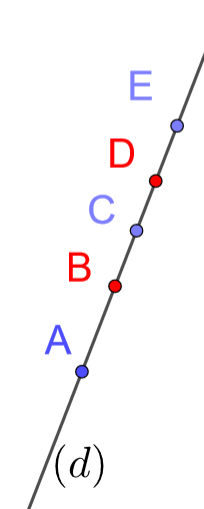
\includegraphics[width=0.35\marginparwidth]{image/axiome_align2.png}\end{center}}

\FigureMarge{Axiome \ref{ax-B2}}{1}{image/axiome_align2.png}


On se donne également l'existence de points entre et à l'\guil{extérieur} d'un couple de points donnés\,: 
\begin{axi}\label{ax-B2}
    Soit $B$ et $D$ deux points distincts, alors il existe des points $A,C$ et $E$ tel que $A\star B \star D$, $B\star C \star D$ et $B\star D \star E$.
    \begin{equation*}
        B,D\in\mathcal{E},\, B,D \text{ distincts } \Rightarrow \exists A,C,E\in\mathcal{E},\, A\star B \star D,\, B\star C \star D\,, B\star D \star E\,.
    \end{equation*}
\end{axi}
Enfin si l'on se donne trois points alignés, une relation \guil{être entre} existe entre ces trois point et è permutation des points extérieurs près, aucune autre relation de ce type n'est établie entre les trois points\,:
\begin{axi}\label{ax-B3}
    Pour trois points distincts sur une même droite, un et un seul est entre les deux autres.
\end{axi}
\begin{exo}
On suppose connues les notions ordinaires de géométrie euclidienne et on se demande si d'autres ensembles de parties peuvent satisfaire les axiomes d'ordre et de congruence. 

Soit $(d)$ une droite dans le plan euclidien, si on note $\mathfrak{C}$, l'ensemble des cercles dont le centre est contenu dans une droite $(d)$ et des droites orthogonales à $(d)$. Montrer que cet ensemble satisfait à tous les axiomes d'incidence (ou l'on remplace \guil{droite} par élément de $\mathfrak{C}$). Expliquer alors pourquoi la relation \guil{être entre} ne peux pas tenir ici.
\end{exo}
Le prochain axiome s'écrit plus aisément si on introduit la notion de segment ouvert\,: 
\begin{defi}[Segment]\label{defi-segment}
Soit $A$ et $B$ deux points distincts, alors on appelle segment ouvert d'extrémité $A$ et $B$ l'ensemble de points
\begin{equation*}
    ]AB[ = \ensemble{M\in\mathcal{E}}{A\star M \star B}\,.
\end{equation*}
De même on définit le segment fermé d'extrémité $A$ et $B$ l'ensemble de point
\begin{equation*}
    [AB] = ]AB[\cup \left\{A,B\right\}\,,
\end{equation*}
et les segments mixtes
\begin{equation*}
    ]AB] = ]AB[\cup \left\{B\right\},\qquad [AB[ = ]AB[\cup \left\{A\right\}\,.
\end{equation*}
\end{defi}
\begin{rema}
    De l'axiome \ref{ax-B1} on déduit que les segments ouverts et fermés sont \guil{non-ordonnés} : $]AB[=]BA[$ et $[AB]=[BA]$.
\end{rema}
L'axiome de Pasch caractérise le nombre d'intersections que fait une droite sécante avec les trois segments qu'on peut construire à l'aide de trois points\,: 
\setcounter{axi}{4}
\begin{axi}[Pasch]\label{ax-pasch}
    Soient trois points distincts et une droite contenue dans un plan tel qu'aucun des trois points n'appartiennent à la droite. Alors soit la droite ne rencontre aucun des segments ouvert formé par les trois points soit elle en rencontre deux (voir figure \ref{fig_pasch}).

    %Plus formellement si on note $\left(]s_i[\right)_{i=1,2,3}$ les trois segments ouverts formé par trois points et $(d)$ une droite ne passant par aucun des trois plan et contenue dans un plan contenant les trois points (et donc également les segments) alors,
    %\begin{equation*}
        %\sum_{i=1,2,3}\mathbf{Card}\left((d)\cap]s_i[\right) = 0 \text{ où } 2\,.
    %\end{equation*}
\end{axi}
\begin{rema}
    Une lecture hâtive de cet axiome peut induire le lecteur en erreur. Le contresens possible est le suivant. Si l'on conçoit un triangle comme la réunion des segments ouverts qui le constituent, alors l'intersection d'un triangle avec une droite est soit vide soit constituée de deux points. L'erreur est ici de n'avoir pas pris en considération les triangles \guil{plats}. Dans ce cas l'intersection avec la réunions des segments ouvert peut être constitué d'un seul point. Et pourtant la droite rencontre deux des segments (l'un est inclus dans l'autre).
\end{rema}
\begin{figure}[h!]
    \centering
    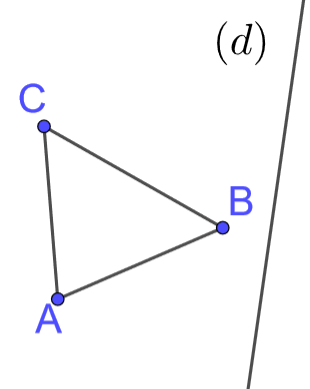
\includegraphics[width=0.3\textwidth]{image/axiome_pasch1.png}\hfill
    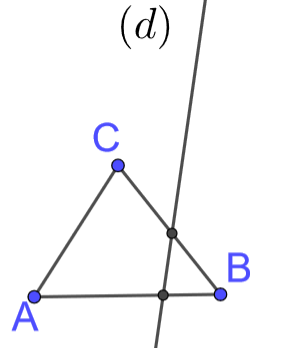
\includegraphics[width=0.3\textwidth]{image/axiome_pasch2.png}
    \caption{Illustration de l'axiome \ref{ax-pasch}. À gauche\,: pas d'intersection. À droite\,: deux intersections. Ne pas oublier que l'axiome interdit que la droite passe par l'un des trois points $A,B$ ou $C$.}
    \label{fig_pasch}
\end{figure}
Le lecteur attentif aura remarqué l'absence de l'axiome B.4. Hilbert l'introduit dans son article original. Cet axiome caractérise les relations \guil{être entre} possibles quand quatre points distincts appartiennent à une même droite. Cet axiome est redondant. C'est-à-dire qu'il peut être démontré à partir des axiomes d'incidence et d'ordre. Pour être tout à fait exact il est redondant si l'axiome de Pasch est formulé en intégrant le cas des triplets de points alignés (comme on l'a fait ici ou dans la publication de Hilbert). La \href{https://www.ams.org/journals/tran/1902-003-01/S0002-9947-1902-1500592-8/S0002-9947-1902-1500592-8.pdf}{preuve} de cette redondance axiomatique est due à Eliakim Hastings et Robert Lee Moore \cite{moore1902projective}, deux mathématiciens Américains homonymes. La preuve est fondée sur quelques lemmes concernant les quadruplets de points alignés dont la preuve repose sur la configuration alignée de l'axiome de Pasch. Ces lemmes nous seront fort utiles et sont présenté en sous-section \ref{subsec-quatrepoints}. L'axiome redondant en question ne nous sera pas utiles. %\addlb{[Ça représente tout de même des pages de démonstrations dans ton bazar...]}

        \subsection{Axiomes de congruences}\setcounter{axi}{0}\setcounter{serieaxiom}{3}

Les axiomes de congruence définissent trois relations dites de congruence entre segments, entre secteurs d'angles ou entre triangles (ces notions sont définies plus loin). Quelques soit le type d'objet considéré (segments, secteurs d'angles et triangles) on notera $\equiv$ la relation de congruence entre deux objets de même nature.

%Une fois les axiomes énumérés, on montrera qu'ils correspondent à l'égalité de mesures des segments (autrement dit, l'isométrie). Cela sera fort utile pour établir des relations entre les mesures d'angles dans la section \ref{subsec_secang}.

Le premier axiome de congruence utilise la notion de demi-droite, ces parties du plan sont definies ainsi\,:
\begin{defi}[Demi-droite]\label{def-demidroite}
    Soit $A$ et $B$ deux points distincts, alors on appelle demi-droite ouverte d'extrémité $A$ contenant $B$ l'ensemble,
    \begin{equation*}
        ]AB) = ]AB] \cup \ensemble{M\in\mathcal{E}}{A\star B \star M}\,.
    \end{equation*}
    et on appelle demi droite fermée d'extrémité $A$ et contenant $B$ l'ensemble,
    \begin{equation*}
        [AB) = ]AB) \cup \left\{A\right\}\,.
    \end{equation*}

    Un ensemble $]d)$ (respectivement $[d)$) est une demi-droite ouverte (respectivement fermé) \ssi il existe $A$ et $B$ distincts tels que $]d)=]AB)$ (respectivement $[d)=[AB)$). On appelle alors $(d)=(AB)$ la droite support des demi-droites $]AB)$ et $[AB)$. 
\end{defi}
\begin{rema}
    Par construction il existe une unique demi-droite (ouverte ou fermée) d'extrémité donnée passant par un point distinct de l'extrémité.
\end{rema}
Le premier axiome pourrait s'appeler axiome du compas, il signifie qu'on peut toujours reporter un segment sur une demi-droite en partant d'une de ses extrémités. Hilbert travaillera avec une droite et définira deux reports possibles. On préfère, pour plus de simplicité par la suite travailler directement avec des demi-droites.
\begin{axi}\label{axi-C1}
    Soit $A$ et $B$ deux points distinct et $]d)$ une demi-droite ouverte d'extrémité $A'$. Alors il existe un unique point $B'$ dans $]d)$ tel que $[AB]$ soit congru à $[A'B']$.
    \begin{align*}
        \forall A,B\in\mathcal{E}, A\neq B,\, \forall ]d) &\text{ demi-droite d'extrémité } A',\, \\
        &\Rightarrow \exists ! B'\in ]d)\,, [AB] \equiv [A'B']\,.
    \end{align*}
\end{axi}
\FigureMarge{Axiome \ref{axi-C1}}{1.2}{image/Axiome_C1.png}
Il paraît conséquent de demander qu'un segment puisse être reporté sur lui-même. De même que si l'un peut être reporté sur le second et que le second peut être reporté sur le troisième alors le premier peut être reporté sur le troisième.
\begin{axi}\label{axi-C2}
    La relation de congruence entre segments est réflexive et transitive.
\end{axi}
\begin{rema} (Rappel)
Une relation binaire $\sim$ sur un ensemble $E$ est une partie de $E\times E$. Plus familièrement deux éléments $x$ et $y$ dans $E$ peuvent être ou ne pas être en relation. Si on note $\sim$ la relation, on notera $x \sim y$ pour signifier\,: \guil{$x$ est en relation avec $y$}. Par exemple pour l'ensemble $\mathfrak{D}$ on peut définir la relation \guil{est parallèle à}. Une relation est dite relation d'équivalence \ssi $\forall x,y,z\in E$\,:
\begin{itemize}[$\bullet$]
    \item elle est symétrique\,:  $x\sim y \Rightarrow y \sim x$,
    \item elle est réflexive\,: $x\sim x$,
    \item et elle est transitive\,:$((x\sim y)\wedge (y\sim z)) \Rightarrow x\sim z$.
\end{itemize}
On vérifie facilement que la relation \guil{est parallèle à} est une relation d'équivalence.
\end{rema}
\begin{rema}
    On peut montrer que $\equiv$ est symétrique. Ainsi, on a le théorème suivant\,:
\end{rema}
\begin{thm}\label{thm-congsegmentequiv}
    La relation de congruence entre segments est une relation d'équivalence.
\begin{proof}
    Il suffit de prouver la symétrie de la relation de congruence entre segments. Soit $A,B,A'$ et $B'$ quatre points tel que $A$ soit distinct de $B$, $A'$ soit distinct de $B'$ et que $[AB]\equiv[A'B']$. On note $]d)=]AB)$. 
    
    L'axiome \ref{axi-C1} implique l'existence d'un point $B''$ sur $]d)$ tel que $[A'B']\equiv[AB'']$. La transitivité (Ax.\ref{axi-C2}) assure,
    \begin{equation*}
        \left\{
        \begin{array}{cc}
             \left[AB\right]&\equiv\left[A'B'\right]  \\
             \left[A'B'\right]&\equiv\left[AB''\right]
        \end{array}
        \right.\quad \Longrightarrow \quad [AB]\equiv[AB'']\,.
    \end{equation*}
    
    Par réflexivité de la relation de congruence entre segment (Ax.\ref{axi-C2}) on a $[AB]\equiv[AB]$, ainsi $B$ et $B''$ sont deux point de la demi-droite $[d)$ d'extrémité $A$ tel que,
    \begin{equation*}
        \left\{
        \begin{array}{cc}
             \left[AB\right]& \equiv \left[AB''\right]  \\
             \left[AB\right]&\equiv \left[AB \right]
        \end{array}
        \right.\,.
    \end{equation*}
    
    Par unicité dans l'axiome \ref{axi-C1} les congruences précédentes assurent $B''=B$ et donc $[A'B']\equiv[AB'']$ devient,
    \begin{equation*}
        [A'B']\equiv[AB]\,,
    \end{equation*}
    ce qui prouve la symétrie de $\equiv$ sur les segments. 
\end{proof}
\end{thm}
La congruence entre segments doit traduire la notion de longueur. Il apparaît alors essentiel d'assurer une forme d'additivité des longueurs sur des points alignés. Cela se traduira par\,:
\begin{axi}\label{axi-C3}
    Soit $(d)$ et $(d')$ deux droites et $A,B,C \in (d)$ tels que $A \star B \star C$ et $A',B',C' \in (d')$ tels que $A' \star B' \star C'$. Alors si $[AB]$ et congru à $[A'B']$ et $[BC]$ et congru à $[B'C']$ alors $[AC]$ et congru à $[A'C']$.
\end{axi}   
\FigureMarge{Axiome \ref{axi-C3}}{1.2}{image/Axiome_C3.png}
Le prochain axiome de congruence traitera de la congruence entre secteurs d'angle saillants. Les secteurs d'angle saillants sont des portions du plan reposant sur la notion de demi-plan\,: 
\begin{defi}[Cotés d'une droite et demi-plan]\label{def-demiplan}
Soit $(d)$ une droite, $A$ et $B$ deux points de $\mathcal{E}$. Alors :
\begin{itemize}[$\bullet$]
    \item Soit $[AB]\cap (d) = \varnothing$ et on dit que $A$ et $B$ \emph{se situent du même coté} de $(d)$.
    \item Soit (exclusif) c'est que $[AB]\cap (d) \neq \varnothing$ et on dit que $A$ et $B$ \emph{se situent de part et d'autre} de $(d)$.
\end{itemize}
On appelle \emph{demi-plan} $\mathcal{P}_{(d),A}$ l'ensemble des points $M$ du plan tel que $M$ et $A$ se situant du même coté de $(d)$. La droite $(d)$ est alors appelé \emph{droite support} du demi plan $\mathcal{P}_{(d),A}$.
\end{defi}
\FigureMarge{Demi-plan \ref{def-demiplan}}{1.2}{image/DemiPlanDefPoint.png}
Une fois définie les demi-plans on peut définir les secteurs d'angle saillant\,: 
\begin{defi}[Secteur d'angle saillant]\label{defi-anglesaillant}
    Soit $I, O$ et $J$ trois points distincts et non alignés, alors on appelle secteur d'\emph{angle saillant} de sommet $O$ entre $]OI)$ et $]OJ)$ l'ensemble des points $M$ tel que $M$ et $J$ soit du même coté de $(OI)$ et que $M$ et $I$ sont du même coté de $(OJ)$. On note alors,
    \begin{equation*}
        \anglesaillant\left({O},{]OI)},{]OJ)}\right) := \mathcal{P}_{(OI),J} \cap \mathcal{P}_{(OJ),I}  
    \end{equation*}
    cet ensemble. %\addlb{[il faudra préciser dans l'intro qu'on note $:=$ les définitions.]}
\end{defi}
\FigureMarge{Secteur d'angle \\ saillant \ref{defi-anglesaillant}}{1.2}{image/SecteurSaillant3ptClair.png}
C'est sur ces ensembles que se définit la prochaine congruence. On demande qu'il n'existe qu'un report de secteur d'angle à partir d'une demi-droite donnée et d'un des demi-plan qu'elle supporte. 
\begin{axi}\label{axi-C4}
    Soient $]d_I)$ et $]d_J)$ deux demi-droites de même extrémité $O$. Soit $]d_I)'$ une demi-droite d'extrémité $O'$ dont la droite support est également celle d'un demi-plan $\mathcal{P}'$, alors il existe une unique demi-droite $]d_J')$ dans $\mathcal{P}'$ d'extrémité $O'$ tel que\,:
    $$\anglesaillant\left(O,]d_I),]d_J)\right)\equiv\anglesaillant\left(O',]d_I'),]d_J')\right)\,.$$
\end{axi}
\FigureMarge{Axiome \ref{axi-C4}}{1.2}{image/Axiome_C4}
Comme pour l'axiome \ref{axi-C1} Hilbert ne precise pas le demi-plan ou on cherche $]d_J')$, il préfère dire qu'il y en a deux. Nous préférons axiomatiser l'unicité par demi-plan afin de s'épargner une lourdeur dans la rédaction des preuves qui suivront. 
\begin{axi}\label{axi-C5}
    La relation de congruence entre angles est transitive et réflexive. 
\end{axi}
On montre de même que pour les segments, que la relation de congruence pour les secteurs d'angles est une relation d'équivalence.
\begin{thm}
    La relation de congruence entre secteurs d'angle est une relation d'équivalence.
\begin{proof}
    La preuve s'effectue de la même manière que celles du théorème \ref{thm-congsegmentequiv}.
\end{proof}
\end{thm}
La prochaine relation d'équivalence concerne les triangles, on définira ces objets \guil{bien connus} comme une suite ordonnée de trois points distincts. 
\begin{defi}[Triangle]
    On appelle \emph{triangle} la donnée de trois points distincts \emph{ordonnées}. Ces points sont appelés sommets du triangle.
\end{defi}
\begin{defi}[Secteur d'angle au sommet d'un triangle]
    Soit $A,B$ et $C$ trois points distincts, on appelle secteurs d'angles du sommet $A$ dans le triangle $ABC$ le secteurs d'angle,
    \begin{equation*}
        \anglesaillant\left(A,]AB),]AC)\right)\,.
    \end{equation*}
\end{defi}
Cette fois-ci cependant la nouvelle congruence (entre triangle) peut être définie positivement, \cad en faisant appelle a des notions déjà connues. 
\begin{defi}[Congruence entre triangles]
    Deux triangles $ABC$ et $A'B'C'$ sont dit congruents \ssi :
    \begin{equation*}
        \left\{
        \begin{array}{ccc}
            [AB] \equiv [A'B']\,, &&  \anglesaillant\left(C,]CA),]CB)\right)\equiv \anglesaillant\left(C',]C'A'),]C'B')\right) \\
            \left[BC\right] \equiv \left[B'C'\right] \,, && \anglesaillant\left(A,]AB),]AC)\right)\equiv \anglesaillant\left(A',]A'B'),]A'C')\right) \\
            \left[CA\right] \equiv \left[C'A'\right]\,, && \anglesaillant\left(B,]BA),]BC)\right)\equiv \anglesaillant\left(B',]B'A'),]B'C')\right)
        \end{array}
        \right.
    \end{equation*}
Autrement dit si tout \guil{leurs angles} et tous leurs \guil{segments} sont congruent deux-à-deux.
\end{defi}
\begin{rema}
    L'ordre des points d'un triangle compte ! En effet si $ABC\equiv A'B'C'$ cela n'implique pas $ABD\equiv B'C'A'$. En effet les congruence à vérifier deux à deux sont déterminées par l'ordre des points. En général $ABC \not \equiv BCA$. 
\end{rema}
\begin{rema}
    Soit $ABC$ un triangle vérifiant $ABC \equiv CBA$ alors ce triangle est isocèle en $B$.
\end{rema}
Il semble que les six congruences à vérifier soient de trop. En effet d'instinct on pense par exemple que si les trois relations de congruence entre segments sont vérifiées, alors il en est de même pour les secteurs d'angle. De même pour un angle et ses côtés adjacents. Ces résultats qualifiés de \guil{cas d'égalité du triangle} ne sont pas démontrables en l'état. Euclide fournit une démonstration bancale de premier cas d'égalité, les autres se déduisant à partir du premier étant correct. Ces cas d'égalités des triangle peuvent être vus comme théorèmes pivots de la géométrie euclidienne. Ne pouvant démontrer rigoureusement le premier, Hilbert en fait un axiome.    
\begin{axi}\label{axi-C6}
    Si deux triangles ont chacun un angle au sommet et les côtés adjacents à ce sommet reliés par une congruence, alors ils sont congruents.
    Autrement dit, si $A_1B_1C_1$ et $A_2B_2C_2$ sont deux triangles tels que les angles aux sommets $A_1$ et $A_2$ sont congruents, alors\,:
    \begin{equation*}
        A_1B_1C_1\equiv A_2B_2C_2\Leftrightarrow((A_1B_1\equiv A_2B_2)\wedge (A_1C_1\equiv A_2C_2))
    \end{equation*}
\end{axi}
\FigureMarge{Axiome \ref{axi-C6}\,: on a codé\\ la congruence de paires\\ d'objets à l'aide\\ des couleurs.}{1.2}{image/tri_cong.png}
%\marginpar{\begin{center}Axiome \ref{axi-C6}\,: on a codé\\ la congruence de paires\\ d'objets à l'aide\\ des couleurs.\\
%    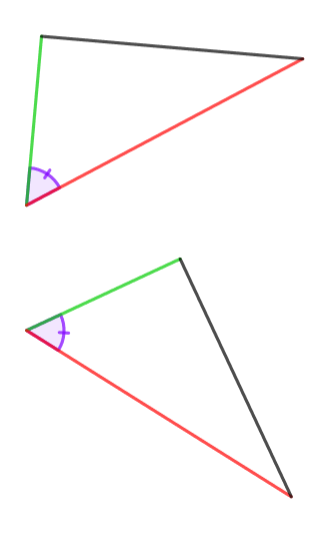
\includegraphics[width=0.5\marginparwidth]{image/tri_cong.png}
%\end{center}}

        \subsection{Axiomes de continuité}\setcounter{axi}{0}\setcounter{serieaxiom}{4}

Les axiomes de continuité vont assurer des propriétés concernant les relations que les points entretiennent entre eux dans l'espace. En particulier, on assurera qu'il est possible de dépasser en taille n'importe quel segment à partir d'un autre, en le reportant un nombre de fois arbitrairement grand.
\begin{defi}[Report]
    Soit $[AB]$ un segment et $]d)$ un demi-droite d'extremité $O$, on appelle report de $[AB]$ sur $]d)$ l'unique point $C$ de $]d)$ tel que $[OC]\equiv [AB]$.
\end{defi}
\begin{rema}
    Par construction le report de $[AB]$ sur $]d)$ est distinct de $O$. 
\end{rema}
Par la suite il sera utile d'établir les résultats suivants.
\begin{prop}
Pour tout points $A$ et $B$ distincts, l'ensemble,
\begin{equation*}
    \ensemble{M\in \mathcal{E}}{A\star B\star M}
\end{equation*}
est une demi-droite d'extrémité $B$.
\begin{proof}
    \addlb{[remarque : pour que tes preuves soient plus lisibles, ne suppose pas que tes lecteurs ont lu 8000 fois ton texte (comme toi) et connaissent par coeur les numéros des théorèmes. Ajoute au moins un petit nom pour rappeler de quoi tu parle. C'est ultra chiant de naviguer en permanence pour se rappeler ce que signifie "axiome B2", "corrolaire 6.2.2" etc.]}

    
    Notons abusivement $]d)$ l'ensemble en question. Soit $C$ dans $]d)$ (existence assuré par l'axiome \ref{ax-B2}). Alors $A\star B\star C$. Le but est alors de montrer que $]d)=]BC)$. 

    Soit $M\in ]d)$ alors on à $A\star B\star M$ et $A\star B\star C$. Si $M=C$ puisque $C\in ]BC)$ sinon on utilise le corollaire \ref{cor-configurationuncote} (dont la démonstration, on l'assure, ne repose que sur les axiomes d'incidence et d'ordre). Ce corollaire assure alors que $B\star M \star C$ (\cad $M\in]AC]$) où $B\star C\star M$ autrement dit $M\in ]BC)$. On en déduit $]d)\subset ]BC)$.

    Soit $M\in ]BC)$ et donc \,:
    \begin{itemize}[$\bullet$]
        \item soit $M=C$ et donc $M \in ]d)$,
        \item soit $M\in ]BC[$ et donc $B\star M\star C$, ce qui, combiné au fait que $A\star B\star C$ conduit d'après le Corollaire.\ref{cor-configurationordrequatrepoint-1} (dont la démonstration, on l'assure, ne repose que sur les axiomes d'incidence et d'ordre) à $A\star B \star M$ et donc $M\in ]d)$.
        \item soit $B \star M \star C$, ce qui combiné au fait que $A\star B\star C$ conduit d'après le Corollaire.\ref{cor-configurationordrequatrepoint-2} (dont la démonstration, on l'assure, ne repose que sur les axiomes d'incidence et d'ordre) à $A\star B \star M$ et donc $M\in ]d)$.
    \end{itemize}
    Dans tout les cas $M\in ]d)$ et donc $]BC)\subset ]d)$.
\end{proof}
\end{prop}
On en déduit en combinant cette proposition avec l'axiome de congruence \ref{axi-C1} que,
\begin{prop}
    Pour tout points $A$ et $B$ distincts et tout segment $[CD]$, il existe un unique point $M$ tel que $A\star B \star M$ et $[CD]\equiv [BM]$. 
\begin{proof}
    Immédiat.
\end{proof}
\end{prop}

On définit alors pour tout $n$ le $n$-report de $[AB]$ sur $]d)$:
\begin{defi}[$n$-Report]
    Soit $[AB]$ un segment, $]d)$ une demi-droite d'extrémité $O$. On construit alors par récurrence la suite de point $\famiin{C}{k}{\N}$ :
    \begin{equation*}
        \left\{\begin{array}{rl}
             C_0 & = O\\
             C_1 & \text{est le report de $[AB]$ sur $]d)$} \\% et $]d_1)$ l'unique demi-droite d'extrémité $C_1$ incluse dans $]d)$}  \\
             C_{n+1} & \text{est l'unique point de $(AB)$ tel que $O\star C_n \star C_{n+1}$ et $[C_n C_{n+1}]\equiv [AB]$}
        \end{array}
        \right.
    \end{equation*}
    Alors pour tout $n\in \N$, le point $C_n$ est appelé $n$-report de $[AB]$ sur $]d)$.
\end{defi}

\begin{rema}
    \added[id=LB]{Ici, on parle de suite (qui plus est, définie par récurrence), alors qu'à aucun moment on n'a expliqué ce que c'était au lecteur. Notre cours est donc incompréhensible.}
\end{rema}

\begin{rema}
    Cette relation de récurrence est bien définie. En effet pour tout $O,C$ deux points distincts, il n'existe qu'une demi-droite d'extrémité $C$ ne contenant pas $O$, cela est une conséquences de l'axiome \ref{axi-A3}. 
\end{rema}
\begin{rema}
    Dans la suite dans le cas ou $O=A$ et $B\in ]d)$ on notera $A+n\overrightarrow{AB}$ le $n$-report de $[AB]$ sur $[AB)$.
\end{rema}
Ces notions vont permettre de formaliser l'axiome d'Archimède. 
\begin{axi}[Archimède]\label{axi-archimede}
    Soit $[AB]$ et $[CD]$ deux segments alors il existe un entier $n$ tel que $E$, le $n$-report de $[CD]$ sur $[AB)$ vérifie $A\star B \star E$. 
\end{axi}

Dans la suite de cette section, on notera,
\begin{equation*}
    \D_+ = \ensemble{\dfrac{n}{2^k}}{(n,k)\in \N_\star\times\N }
\end{equation*}
\addlb{Vu qu'on n'a jamais parlé de produit cartésien, il vaut mieux bannir cette notation et mettre $n\in\N_\star, k\in\N$.}
l'ensemble des nombre diadique. Dans la logique de Dedekind, on rappelle (ou pas) que pour toute partition,
\begin{equation*}
    \D_1 \cap \D_2 = \D_+ 
\end{equation*}
non vide de $\D_+$, telle que,
\begin{equation*}
    \forall (d_1,d_2)\in \D_1 \times \D_2\,, \text{ on ai } d_1 < d_1
\end{equation*}
il existe un unique nombre réel $x\in \R_+^\star$ tel que,
\begin{equation*}
    \forall (d_1,d_2)\in \D_1 \times \D_2\,, \text{ on ai } d_1 \leq x \leq d_1\,.
\end{equation*}
$x$ est alors le plus petit majorant de $\D_1$ ou symétriquement le plus grand majorant de $\D_2$. 

Les axiomes précédent ne sont pas suffisants pour assurer que l'espace \guil{ne contient pas de trou} (voir Exo. \ref{exo-constructible}). L'axiome suivant assurera alors à l'espace cette propriété. 
\begin{axi}[Dedekind]\label{axi-dedekind}
    Soit $]d)$ une demi-droite ouvert d'extrémité $O$ qui est la partition en deux ensemble $\Sigma_-$ et $\Sigma_+$ et tel que $\forall (A_-,A_+)\in \Sigma_-\times \Sigma_+$ on ai $O\star A_- \star A_+$. Alors il existe un unique point $X$ tel que $\forall (A_-,A_+)\in \Sigma_-\times \Sigma_+$ on ai $ A_- \star X \star A_+$.
\end{axi}
Hilbert n'énonce pas cet axiome et préfère énoncer un axiome équivalent dit de l'intégrité linéaire. 

Néanmoins sa formulation \guil{méta} nous a conduit a préféré cette formulation. 
\addlb{[incompréhensible et (donc) inutile si tu ne cites pas ledit axiome. Je propose de supprimer cette remarque.]}

\begin{exo}\label{exo-constructible}
On se place dans $\R^2$ \addlb{On n'a jamais défini $\R^2$!!!}, et on cherche a savoir si la sous-partie des points dit constructible peut satisfaire à tout les axiomes de Hilbert. 

Les points dit constructibles sont définis comme points issus d'une succession finie d'étapes\addlb{, \guil{à la règle non graduée et au compas}, c'est-à-dire de la manière suivante}. Soit une sous partie $E\subset \R^2$, on dit qu'un point $M$ est constructible \emph{en une étape} a partir de $E$ \ssi $M\in E$ ou si $E$ est l'intersection de partie du type :
\begin{itemize}[$\bullet$]
    \item un droite définie par deux points distincts de $E$\,;
    \item un cercle dont le centre est dans $E$ est dont le rayon est un segment formé par deux point distincts de $E$\,
\end{itemize} 
On note alors $\mathfrak{T}_1\left(E\right)$ l'ensemble des points contructibles à partir de $E$. On a bien évidement $E\subset \mathfrak{T}\left(E\right)$. On étend alors par récurrence $\mathfrak{T}_{n+1}\left(E\right):=\mathfrak{T}_1\left(\mathfrak{T}_n\left(E\right)\right)$ l'ensemble des points constructibles en $n$ étapes à partir de $E$. Enfin on définit l'ensemble des nombres constructibles à partir de $E$ comme l'ensemble des points $M$ tel qu'il existe $n\in\N$ tel que $M\in \mathfrak{T}_n\left(E\right)$ et on notera $\mathcal{T}\left(E\right)$ l'ensemble des points constructibles à partir de $E$.

On se donne deux points distincts $O=(0,0)$ et $I=(0,1)$ et on note $\mathfrak{T}\left(\{O,I\}\right)=\mathfrak{T}$
\begin{enumerate}
    \item Discuter du fait que $\Z^2 \subset \mathfrak{T}$.
    \item De même argumenter $\Q^2 \subset \mathfrak{T}$.
    \item Montrer que $\mathfrak{T}$ est strictement plus grand que $\Q^2$. \addlb{[définis "plus grand que".]}
    \item $\mathfrak{T}$ respecte-t-il tout les axiomes de Hilbert (a l'exception de l'axiome de Dedekind)? 
    \item Sachant que $(\pi,0)\notin \mathfrak{T}$ en déduire que $\mathfrak{T}$ ne respecte pas l'axiome de Dedekind. 
\end{enumerate}
\end{exo}

        \subsection{Axiome des parallèles}

Enfin il y a l'axiome qui a été le plus discuté\,: l'axiome des parallèles.

\begin{defi}[Droites parallèles]
    Deux droites $(d_1)$ et $(d_2)$ sont \emph{parallèles} \ssi $(d_1)\cap (d_2) = \varnothing$. On note alors $(d_1)\|(d_2)$. 
\end{defi}        
\begin{defi}[Droites sécantes]\label{def-secantes}
    Deux droites distinctes sont dites \emph{sécantes} \ssi leurs intersection est non vide.
\end{defi}
\begin{thm}[Droites sécantes]\label{thm-droitesecante}
    L'intersection deux deux droites sécantes est réduite à un point.
\end{thm}
\begin{proof}
    Si cette intersection étais composé de plus d'un point alors l'axiome (\ref{axi-A1}) impliquerait que ces deux droites soient identiques\,: non distinctes. Contradiction.
\end{proof}
\begin{axi}[Des parallèle]\label{axi-parra}
    Pour toute droite $(d)$ et pour tout point $P$ de $\mathcal{E}-(d)$ il existe une unique droite $(d')$ parallèle à $(d)$ et contenant $P$.
\end{axi}

L'exposé des axiomes est terminé. Il est maintenant temps de s'attaquer à ces longues chaînes de raisons qui donnaient a Descartes l'idée\guil{que toutes les choses qui peuvent tomber sous la connaissance des hommes s'entresuivent en même façon}.

%\epigraph{Ces longues chaînes de raison, si simples et faciles, dont les géomètres ont coutume de se servir pour parvenir à leurs plus difficiles démonstrations, m'avaient donné occasion de m'imaginer que toutes les choses qui peuvent tomber sous la connaissance des hommes s'entresuivent en même façon.}{Descartes, Discours de la méthode.}

    \section{Résultats et constructions préalables}
    \addlb{[Ce titre sent le moisi.]}

    L'objet de cette section est d'établir quelques résultats relativement proches des axiomes et qui nous serviront tout aux long du chapitre \ref{chap_angle}.

    \addlb{[Ici tu répètes exactement ce que dit le titre... ça ne nous avance pas.]}


        \subsection{Résultat sur l'ordonnancement de quatre points}\label{subsec-quatrepoints}


\replaced[id=LB]{Cette partie contient}{Les résultats de cette partie concernent} des résultats primordiaux sur l'ordonnancement à quatre points. Énoncés extrêmement évidents sur des dessins, leurs démonstration à partir des axiomes est laborieuse. Nous conseillons aux lecteurs de passer les démonstrations et de lire néanmoins les énoncés des lemmes et corollaires en première lecture.  Ces résultats sont les fondations de la \href{https://www.ams.org/journals/tran/1902-003-01/S0002-9947-1902-1500592-8/S0002-9947-1902-1500592-8.pdf}{preuve} de l'\guil{axiome B4} par les américains Hastings Moore et Robert Lee Moore. Les lemmes y démontrent des suites d'alignements impossibles en vertu de la configuration plate de l'axiome de Pasch (Ax. \ref{ax-pasch}). Les corollaires énoncent les déductions qui serviront dans des cas plus pratiques.

%\footnote{\url{https://www.ams.org/journals/tran/1902-003-01/S0002-9947-1902-1500592-8/S0002-9947-1902-1500592-8.pdf}}
    %Le lecteur attentif aura remarqué l'absence de l'axiome B.4. Dans son article original, Hilbert ajoute un quatrième axiome qui est en fait redondant, \cad qu'il peut être démontré à l'aides des axiomes (de \ref{axi-A1} à \ref{axi-A3} et \ref{ax-B1},\ref{ax-B2} et \ref{ax-pasch}). Pour être tout-à-fait exact, il est redondant si l'axiome de Pasch est formulé en intégrant le cas des triplets de points alignés (comme on l'a fait ici ou dans la publication de Hilbert). La \href{https://www.ams.org/journals/tran/1902-003-01/S0002-9947-1902-1500592-8/S0002-9947-1902-1500592-8.pdf}{preuve} de cette redondance axiomatique est due à Eliakim Hastings Moore et Robert Lee Moore deux mathématiciens Américains homonyme. La preuve est fondée sur quelques Lemme concernant les quadruplets de points alignés. La preuve de ces lemmes repose sur la configuration alignée des trois points de l'axiome de Pasch.

    %Nous ne présenterons ici certains des lemmes intervenants dans cette preuve car ils s'avèrent utile dans le reste de notre contruction. Il pourra sembler au lecteur que nous prouvons ici des évidences. La lecture des preuve pourra être passée en première lecture, elle offre néanmoins une jolie illustration de la puissance de l'axiome de Pash.

\begin{lem}[Impossibilité cyclique]\label{lem-Impossibilitecyclique}
    Soit $\fami{A}{i}{1,2,3,4}$ quatre points distincts appartenant à une même droite. Alors les systèmes de relation, dit cycliques et pseudo-cycliques,
        \begin{equation*}
        \left\{
            \begin{array}{c}
                 A_{1} \star A_{2} \star A_{3} \\
                 A_{2} \star A_{3} \star A_{4}\\
                 A_{3} \star A_{4} \star A_{1}\\
            \end{array}
            \right. 
             \quad\text{ ou }\qquad \left\{
            \begin{array}{c}
                 A_{1} \star A_{2} \star A_{3} \\
                 A_{2} \star A_{3} \star A_{4}\\
                 A_{4} \star A_{1} \star A_{3}\\
            \end{array}
            \right.
            \,.
    \end{equation*}
    sont impossibles. 
    \begin{proof}
        Les deux premières relations des deux systèmes sont les même. On commencera par supposer vrai uniquement ces deux première relations.
    
        Notons $(d_s)=(A_i A_j)$ pour $i\neq j = 1,2,3,4$, $]s_1[=]A_2 A_4[$, $]s_2[=]A_1 A_2[$ et enfin $]s_3[=]A_1 A_4[$. 

        L'axiome \ref{axi-A3} permet alors l'existence d'un point en dehors de $(d_s)$. On note $(d)=(A_3 A)$.  Par construction $(d)$ et $(d_s)$ sont sécante d'intersection $B_3$.

        Puisque $A_{2} \star A_{3} \star A_{4}$, $A_3\in ]s_1[$ et donc $(d)\cap ]s_1[$ vaut donc $A_3$ car il contient $A_3$ et qu'il est composé d'au plus un point puisque inclus dans l'intersection des droites sécantes $(d)$ et $(d_s)$. Son cardinal est égale à $1$

        $A_3 \notin ]s_2[ = ]A_1 A_2[$ car si c'était le cas, cela impliquerai $A_1 \star A_3 \star A_2$ qui est (en vertu de l'axiome \ref{ax-B3}) en contradiction avec $A_{1} \star A_{2} \star A_{3}$. Le cardinal de $(d)\cap]s_2[$ est donc $0$.

        La droite $(d)$ n'étant pas confondus avec $(d_s)$ est n'est pas confondus avec aucune des droites supports des segments ouverts $]s_1[,]s_2[$ et $]s_3[$. 

        De plus $(d)$ ne passe ni par $A_1,A_2$ ou $A_4$ puisque vue que les points $\fami{A}{i}{1,2,3,4}$ sont distinct cela impliquerai que $(d)$ et $(d_s)$ soit confondus ce qui est exclut par construction de $(d)$.

        On peut donc appliquer l'axiome de Pasch \ref{ax-pasch} au triplet $A_1,A_2$ et $A_4$ et à la droite $(d)$. On en déduit que,
        \begin{equation*}
            (d)\cap]s_3[\neq \varnothing\,.
        \end{equation*}
        or puisque $(d)\cap]s_3[ \subset (d)\cap (d_s) = \left\{B_3 \right\}$ et donc $(d)\cap]s_3[ = \left\{B_3 \right\}$ ce qui implique que $B_3 \in ]s_3[ = ]A_1 A_4[$ ce qui implique encore que $A_1 \star A_3 \star A_4$. 
        
        Dans le cas ou c'est le premier système qui est supposer vrai $A_1 \star A_3 \star A_4$ entre en contradiction (en vertu de l'axiome \ref{ax-B3}) avec $A_{3} \star A_{4} \star A_{1}$. Contradiction.

        Dans le cas ou c'est le premier système qui est supposer vrai $A_1 \star A_3 \star A_4$ entre en contradiction (en vertu de l'axiome \ref{ax-B3}) avec $A_{4} \star A_{1} \star A_{3}$. Contradiction.

        Les deux systèmes sont impossibles.
    \end{proof}
\end{lem}
\begin{rema}
    La dénomination cyclique pour une tel système de relation entre points est justifié car chacune des relations se déduit des autre en appliquant un 4-cycle. 
\end{rema}
\begin{rema}
    Ce puissant lemme \ref{lem-Impossibilitecyclique} est une sorte d'extension à quatre points de l'axiome \ref{ax-B3}. Vue la fréquence de l'usage de \ref{ax-B3}, on comprend tout l'intérêt d'un tel résultat.
\end{rema}
\begin{cor}\label{cor-configurationordrequatrepoint-1}
Soit $\fami{A}{i}{1,2,3,4}$ quatre points distincts appartenant à une même droite. Alors on a,
        \begin{equation*}
        \left\{
            \begin{array}{c}
                 A_{1} \star A_{2} \star A_{3} \\
                 A_{2} \star A_{3} \star A_{4}\\
            \end{array}
            \right. \quad \Longrightarrow \quad \left\{
            \begin{array}{c}
                A_1 \star A_3 \star A_4\\
                A_1 \star A_2 \star A_4
            \end{array}
            \right.\,.
    \end{equation*}
    \begin{proof}
        Les trois points $A_1,A_3$ et $A_4$ sont alignés alors l'axiomes \ref{ax-B3} implique que,
        \begin{equation*}
            A_1 \star A_3 \star A_4 \quad\text{où}\quad A_3 \star A_4 \star A_1 \quad\text{où}\quad A_4 \star A_1 \star A_3 
        \end{equation*}
        (où exclusif) or les deux dernières options sont exclue en vertu du Lemme \ref{lem-Impossibilitecyclique}. La seule possibilité restante étant $A_1 \star A_3 \star A_4$

        De même les trois points $A_1,A_2$ et $A_4$ sont alignés alors l'axiomes \ref{ax-B3} implique que,
        \begin{equation*}
            A_1 \star A_2 \star A_4 \quad\text{où}\quad A_2 \star A_4 \star A_1 \quad\text{où}\quad A_4 \star A_1 \star A_2 
        \end{equation*}
        (où exclusif) or les deux dernières options (en renommant les points) font apparaître les systèmes de relations cyclique et pseudo-cycliques et sont donc excluent (en vertu du Lemme \ref{lem-Impossibilitecyclique}). En effet si la seconde (troisième) option est retenue on obtient les systèmes de relations,
        \begin{equation*}
        \begin{array}{cccc}
        \text{Option 2 }:&\left\{
            \begin{array}{cc}
                 A_{1} \star A_{2} \star A_{3} \\
                 A_{2} \star A_{3} \star A_{4} \\
                 A_2 \star A_4 \star A_1
            \end{array}
            \right. &\qquad\text{Option 3 } :&    \left\{\begin{array}{c}
                 A_{1} \star A_{2} \star A_{3} \\
                 A_{2} \star A_{3} \star A_{4} \\
                 A_4 \star A_1 \star A_2
            \end{array}\right.
        \end{array} \,.
        \end{equation*}
        En renommant les points via $(A_1,A_2,A_3,A_4)=( B_4,B_3,B_2,B_1)$ puis en utilisant la symétrie de la relation \guil{être entre} issue de l'axiome \ref{ax-B1} dans le premier système, et en renommant les points $(A_1,A_2,A_3,A_4)=(C_2,C_3,C_4,C_1)$ dans le second système les systèmes deviennent,
        \begin{equation*}
        \begin{array}{cccc}
        \text{Option 2 }:&\left\{
            \begin{array}{c}
                 B_{2} \star B_{3} \star B_{4} \\
                 B_{1} \star B_{2} \star B_{3} \\
                 B_4 \star B_1 \star B_3
            \end{array}
            \right. &\qquad\text{Option 3 } :&    \left\{\begin{array}{c}
                 C_2 \star C_3 \star C_4 \\
                 C_3 \star C_4 \star C_1 \\
                 C_1 \star C_2 \star C_3
            \end{array}\right.
        \end{array} \,.
        \end{equation*}
        ce qui permet d'identifier le système de droite comme pseudo-cyclique et le système de gauche comme cyclique et donc tout deux impossible.
        
        La seule possibilité restante étant $A_1 \star A_2 \star A_4$.
    \end{proof}
\end{cor}
\begin{lem}[Un point n'est pas entre tout les autres]\label{lem-impossibiliteunpointentretous}
Soit $\fami{A}{i}{1,2,3,4}$ quatre points distincts appartenant à une même droite. Alors
    \begin{equation*}
        \left\{
            \begin{array}{c}
                 A_{1} \star A_{4} \star A_{2} \\
                 A_{2} \star A_{4} \star A_{3}\\
                 A_{3} \star A_{4} \star A_{4}\\
            \end{array}
            \right. 
    \end{equation*}
est impossible.
    \begin{proof}
        On construit comme dans la preuve précédente une droite sécantes à la droite $(d_s)=(A_i A_j)$ (pour $i\neq j$), mais cette fois ci passant par $A_4$. 
        
        Alors les relations supposé conduisent au fait que $A_4\in ]A_1,A_2[$,   $A_4\in ]A_2,A_3[$ et $A_4\in ]A_3,A_1[$ et donc que chaque intersection $(d)\cap ]A_1,A_2[$, $(d)\cap ]A_2,A_3[$, $(d)\cap ]A_2,A_3[$ contient au moins $A_4$ ($A_4\in (d)$ par construction de $(d)$).

        Ainsi,
        \begin{equation*}
           \mathbf{Card}\left((d)\cap]A_1,A_2[\right)+\mathbf{Card}\left((d)\cap]A_2,A_3[\right)+\mathbf{Card}\left((d)\cap]A_3,A_1[\right) \geq 3
        \end{equation*}

        $(d)$ ne passe par aucun des points $A_1,A_2$ et $A_3$ car puisque ces points sont distincts de $A_4$ si $(d)$ passait par l'un deux elle serait confondus avec $(d_s)$ ce qui n'est pas le cas par construction de $(d)$.

        On peut donc appliquer l'axiome de Pasch \ref{ax-pasch} à $(d)$ et au segments ouverts $]A_1,A_2[$, $ ]A_2,A_3[$ et $ ]A_3,A_1[$ et alors,
        \begin{equation*}
            \mathbf{Card}\left((d)\cap]A_1,A_2[\right)+\mathbf{Card}\left((d)\cap]A_2,A_3[\right)+\mathbf{Card}\left((d)\cap]A_3,A_1[\right) = 0 \text{ ou }2\,.
        \end{equation*}
        ce qui entre en contradiction avec la relation précédentes.
    \end{proof}
\end{lem}
\begin{cor}\label{cor-configurationordrequatrepoint-2}
Soit $\fami{A}{i}{1,2,3,4}$ quatre points distincts appartenant à une même droite. Alors on a,
        \begin{equation*}
        \left\{
            \begin{array}{c}
                 A_{1} \star A_{2} \star A_{4} \\
                 A_{2} \star A_{3} \star A_{4}\\
            \end{array}
            \right. \quad \Longrightarrow \quad \left\{
            \begin{array}{c}
                A_1 \star A_2 \star A_3\\
                A_1 \star A_3 \star A_4
            \end{array}
            \right.\,.
    \end{equation*}
    \begin{proof}
        Les points $A_1,A_3$ et $A_4$ sont alignés alors l'axiome \ref{ax-B3} implique que,
        \begin{equation*}
            A_1 \star A_3 \star A_4 \quad\text{où}\quad A_3 \star A_4 \star A_1 \quad\text{où}\quad A_4 \star A_1 \star A_3 
        \end{equation*}
        (où exclusif). On montre que les deux dernières options sont exclus. 

        Si \textbf{la seconde option} $A_3 \star A_4 \star A_1$ est retenue pour $A_1,A_3$ et $A_4$ alors on obtient le système de relation,
        \begin{equation*}
        \left\{
            \begin{array}{c}
                 A_1 \star A_2 \star A_4 \\
                 A_2 \star A_3 \star A_4 \\
                 A_3 \star A_4 \star A_1 
            \end{array}
            \right. \,.
        \end{equation*}
        dont les deux dernières conduisent en vertu du Corollaire \ref{cor-configurationordrequatrepoint-1} à deux autres relations et donc au système,
        \begin{equation*}
        \left\{
            \begin{array}{c}
                 A_1 \star A_2 \star A_4 \\
                 A_2 \star A_3 \star A_4 \\
                 A_3 \star A_4 \star A_1 \\
                 A_2 \star A_3 \star A_1 \\
                 A_2 \star A_4 \star A_1 
            \end{array}
            \right. \,.
        \end{equation*}
        or ce système est impossible car, en vertu de l'axiome \ref{ax-B3} la première et la dernière relation de ce système se contredisent. La seconde option est exclus.

        \textbf{Si la troisième option} $A_4 \star A_1 \star A_3$ est retenue pour $A_1,A_3$ et $A_4$ alors on obtient le système de relation,
        \begin{equation*}
        \left\{
            \begin{array}{c}
                 A_1 \star A_2 \star A_4 \\
                 A_2 \star A_3 \star A_4 \\
                 A_4 \star A_1 \star A_3 
            \end{array}
            \right. \,.
        \end{equation*}
        Les points $A_1,A_2$ et $A_3$ étant également alignés l'axiome \ref{ax-B3} implique que, 
        \begin{itemize}[$\bullet$]
            \item Soit $A_2 \star A_3 \star A_1$ et alors on a le système de relation,
            \begin{equation*}
            \left\{
            \begin{array}{c}
                 A_1 \star A_2 \star A_4 \\
                 A_2 \star A_3 \star A_4 \\
                 A_4 \star A_1 \star A_3 \\
                 A_2 \star A_3 \star A_1
            \end{array}
            \right. \,.
            \end{equation*}
            dont les deux dernières implique (Corollaire \ref{cor-configurationordrequatrepoint-1}) $A_2 \star A_1 \star A_4$ et $A_2 \star A_3 \star A_4$. Or $A_2 \star A_1 \star A_4$ vient contredire la première relation du système précédent (axiome \ref{ax-B3}). $A_2 \star A_3 \star A_1$ est impossible.
            \item Soit $A_3 \star A_1 \star A_2$ et alors on a le système de relation,
            \begin{equation*}
            \left\{
            \begin{array}{c}
                 A_1 \star A_2 \star A_4 \\
                 A_2 \star A_3 \star A_4 \\
                 A_4 \star A_1 \star A_3 \\
                 A_3 \star A_1 \star A_2
            \end{array}
            \right. \,.
            \end{equation*}
            alors le première est la dernière relation implique (Corollaire \ref{cor-configurationordrequatrepoint-1}) $A_3 \star A_1 \star A_4$ et $A_3 \star A_2 \star A_4$. Or  $A_3 \star A_1 \star A_4$ et $A_3 \star A_2 \star A_4$ vient contredire la deuxième relation du système précédent (axiome \ref{ax-B3}). $A_3 \star A_1 \star A_2$ est impossible.
            \item Soit $A_1 \star A_2 \star A_3$ et alors le système devient,
            \begin{equation*}
            \left\{
            \begin{array}{c}
                 A_1 \star A_2 \star A_4 \\
                 A_2 \star A_3 \star A_4 \\
                 A_4 \star A_1 \star A_3 \\
                 A_1 \star A_2 \star A_3
            \end{array}
            \right. \,.
            \end{equation*}
            on remarque alors que les trois dernière relations de ce système forme un système pseudo-cyclique dont l'impossibilité à déja été démontré (Lemme \ref{lem-Impossibilitecyclique}). 
        \end{itemize}
        aucun choix n'est possible concernant l'arrangement des points $A_1,A_2$ et $A_3$. La seconde option est impossible.

        On en déduit que la première option est la seule possible alors on a,
        \begin{equation*}
            \left\{
            \begin{array}{c}
                 A_1 \star A_2 \star A_4 \\
                 A_2 \star A_3 \star A_4 \\
                 A_1 \star A_3 \star A_4 
            \end{array}
            \right. \,.
        \end{equation*}
        $A_1,A_2$ et $A_3$ étant également alignés l'axiome \ref{ax-B3} implique que, 
        \begin{itemize}[$\bullet$]
            \item Soit $A_3 \star A_1 \star A_2 = A_2 \star A_1 \star A_3$. Alors le système devient,
            \begin{equation*}
            \left\{
            \begin{array}{c}
                 A_1 \star A_2 \star A_4 \\
                 A_2 \star A_3 \star A_4 \\
                 A_1 \star A_3 \star A_4 \\
                 A_2 \star A_1 \star A_3
            \end{array}
            \right. \,,
            \end{equation*}
            dont les deux dernières relations implique (Lemme \ref{cor-configurationordrequatrepoint-1}) que $A_2 \star A_1 \star A_4$ et $A_2 \star A_3 \star A_4$. Or $A_2 \star A_1 \star A_4$ vient contredire (Axiome \ref{ax-B3}) la première relation du sytème. Contradiction : $A_3 \star A_1 \star A_2$ est impossible.
            \item Soit $A_2 \star A_3 \star A_1$ et alors le système devient,
            \begin{equation*}
            \left\{
            \begin{array}{c}
                 A_1 \star A_2 \star A_4 \\
                 A_2 \star A_3 \star A_4 \\
                 A_1 \star A_3 \star A_4 \\
                 A_2 \star A_3 \star A_1
            \end{array}
            \right. \,,
            \end{equation*}
            dont les trois dernière relations sont impossible en vertu du Lemme \ref{lem-impossibiliteunpointentretous}.
        \end{itemize}
        On en déduit que seule $A_1 \star A_2 \star A_3$ est possible. On a donc,
        \begin{equation*}
        \left\{
            \begin{array}{c}
                 A_{1} \star A_{2} \star A_{4} \\
                 A_{2} \star A_{3} \star A_{4}\\
            \end{array}
            \right. \quad \Longrightarrow \quad \left\{
            \begin{array}{c}
                A_1 \star A_2 \star A_3\\
                A_1 \star A_3 \star A_4
            \end{array}
            \right.\,.
    \end{equation*}
    \end{proof}
\end{cor}
\begin{cor}\label{cor-configurationuncote}
    Soit $\fami{A}{i}{1,2,3,4}$ quatre points distincts d'une même droite $(d)$ alors,
    \begin{equation*}
        \left\{
        \begin{array}{cc}
             A_1 \star A_2 \star A_3  \\
             A_1 \star A_2 \star A_4 
        \end{array}
        \right. \quad \Longrightarrow \quad       
        \left\{\begin{array}{cc}
             A_2 \star A_3 \star A_4  \\
             A_1 \star A_3 \star A_4 
        \end{array}\right. \quad \text{ou} \quad
        \left\{\begin{array}{cc}
             A_2 \star A_4 \star A_3  \\
             A_1 \star A_4 \star A_3 
        \end{array}\right.\,.
    \end{equation*}
    \begin{proof}
        Puisque les triplés $\left\{A_2,A_3,A_4\right\}$ et $\left\{A_1,A_3,A_4\right\}$ sont deux triplés de points alignés l'axiome \ref{ax-B3} implique qu'on ai,
        \begin{equation*}
            \begin{array}{cccccc}
                 \left\{A_1,A_2,A_3\right\}\,:\,& A_2 \star A_3 \star A_4 \,(a) & \text{ou} & A_2 \star A_4 \star A_3 \,(b) & \text{ou} & A_4 \star A_2 \star A_3 \,(c) \\
                 \left\{A_2,A_3,A_4\right\}\,:\,& A_1 \star A_3 \star A_4 \,(a) & \text{ou} & A_1 \star A_4 \star A_3 \,(b) & \text{ou} & A_3 \star A_1 \star A_4 \,(c) \\
            \end{array}
        \end{equation*}
        (ou exclusif). Il s'agit de montrer que les configurations $(ab),(ba)$, $(xc)$ (pour $x=a,b,c$) et $(cx)$ (pour $x=a,b,c$) sont impossible.

        \begin{itemize}[$\bullet$]
            \item Montrons que $(cx)$ (pour $x=a,b,c$) est impossible. Si c'était le cas, on aurait le système de relation,
            \begin{equation*}
                \left\{\begin{array}{cc}
                     A_1 \star A_2 \star A_3  \\
                     A_1 \star A_2 \star A_4  \\
                     A_4 \star A_2 \star A_3
                \end{array}\right.\,,
            \end{equation*}
            qui est impossible en vertu du Lemme \ref{lem-impossibiliteunpointentretous}. $(cx)$ (pour $x=a,b,c$) est impossible.
            \item Montrons que $(xc)$ (pour $x=a,b,c$) est impossible. Si c'était le cas, on aurait le système de relation,
            \begin{equation*}
                \left\{\begin{array}{cc}
                     A_1 \star A_2 \star A_3  \\
                     A_1 \star A_2 \star A_4  \\
                     A_3 \star A_1 \star A_4
                \end{array}\right.\,,
            \end{equation*}
            dont la deuxième et la troisième relation implique (Corollaire \ref{cor-configurationordrequatrepoint-2} que $A_3 \star A_1 \star A_2$ et $A_3 \star A_2 \star A_4$. Or $A_3 \star A_1 \star A_2$ vient contredire $A_1 \star A_2 \star A_3$ (axiome \ref{ax-B3}). $(xc)$ (pour $x=a,b,c$)  est impossible.
            \item Montrons que $(ab)$ est impossible. Si c'était le cas, on aurait le système de relation,
            \begin{equation*}
                \left\{\begin{array}{cc}
                     A_1 \star A_2 \star A_3  \\
                     A_1 \star A_2 \star A_4  \\
                     A_2 \star A_3 \star A_4 \\
                     A_1 \star A_4 \star A_3
                \end{array}\right.\,,
            \end{equation*}
            dont la première et la troisième relation implique (Corollaire \ref{cor-configurationordrequatrepoint-1} que $A_1 \star A_2 \star A_4$ et $A_1 \star A_3 \star A_4$. Or $A_1 \star A_3 \star A_4$ vient contredire $A_1 \star A_4 \star A_3$ (axiome \ref{ax-B3}). $(ab)$ est impossible.
            \item Montrons que $(ba)$ est impossible. Si c'était le cas, on aurait le système de relation,
            \begin{equation*}
                \left\{\begin{array}{cc}
                     A_1 \star A_2 \star A_3  \\
                     A_1 \star A_2 \star A_4  \\
                     A_3 \star A_4 \star A_2 \\
                     A_1 \star A_3 \star A_4
                \end{array}\right.\,,
            \end{equation*}
            dont la troisième et la quatrième relation implique (Corollaire \ref{cor-configurationordrequatrepoint-1} que $A_1 \star A_3 \star A_2$ et $A_1 \star A_4 \star A_2$. Or $A_1 \star A_3 \star A_2$ vient contredire $A_1 \star A_2 \star A_3$ (axiome \ref{ax-B3}). $(ba)$ est impossible.
        \end{itemize}
        Les seules possibilité restantes sont $(aa)$ ou $(bb)$. Ce qui prouve l'implication.
    \end{proof}
\end{cor}
\begin{cor}\label{cor-configurationordrequatrepoint-3}
    Soit $\fami{A}{i}{1\ldots 4}$ quatre points distincts appartenant à une même droite $(d)$, alors,
    \begin{equation*}
        \left\{
            \begin{array}{c}
                 A_1 \star A_2 \star A_3 \\
                 A_1 \star A_3 \star A_4
            \end{array}
            \right. \quad \Longleftrightarrow \quad \left\{
            \begin{array}{c}
                A_1 \star A_2 \star A_4\\
                A_2 \star A_3 \star A_4
            \end{array}
            \right.
            \,.
    \end{equation*}
    \begin{proof}
        Les points $A_2,A_3$ et $A_4$ sont alignés alors l'axiome \ref{ax-B3} implique que,
        \begin{equation*}
            A_2 \star A_3 \star A_4 \quad\text{où}\quad A_3 \star A_4 \star A_2 \quad\text{où}\quad A_4 \star A_2 \star A_3 \,,
        \end{equation*}
        (où exclusif). On commence par montrer que la seconde et la troisième options sont impossible. 
        
        \textbf{Option 2 ($A_3 \star A_4 \star A_2$) :}  Si la seconde option est choisit on obtient le système,
        \begin{equation*}
        \left\{
            \begin{array}{c}
                 A_1 \star A_2 \star A_3 \\
                 A_1 \star A_3 \star A_4 \\
                 A_3 \star A_4 \star A_2 
            \end{array}
            \right. \,,
        \end{equation*}
        on peut alors utiliser le Corrolaire \ref{cor-configurationordrequatrepoint-1} sur les deux dernière relations pour obtenir deux autres relations. Et aboutir aux système.
        \begin{equation*}
        \left\{
            \begin{array}{c}
                 A_1 \star A_2 \star A_3 \\
                 A_1 \star A_3 \star A_4 \\
                 A_3 \star A_4 \star A_2 \\
                 A_1 \star A_3 \star A_2 \\
                 A_1 \star A_4 \star A_2 
            \end{array}
            \right. \,,
        \end{equation*}
        dont la première et quatrième relations sont en contradictions en vertu de l'axiome \ref{ax-B3}.

        \textbf{Option 3 ($A_4 \star A_2 \star A_3$) :} Si la troisième option est choisit on obtient le système,
        \begin{equation*}
        \left\{
            \begin{array}{c}
                 A_1 \star A_2 \star A_3 \\
                 A_1 \star A_3 \star A_4 \\
                 A_4 \star A_2 \star A_3 
            \end{array}
            \right. \,,
        \end{equation*}
        on examine alors les possibilités pour le triplé de points alignés $A_1,A_2$ et $A_4$ (axiome \ref{ax-B3}), on a :
        \begin{itemize}[$\bullet$]
            \item Soit $A_1 \star A_2 \star A_4$ alors on à le système de relation,
            \begin{equation*}
            \left\{
            \begin{array}{c}
                 A_1 \star A_2 \star A_3 \\
                 A_1 \star A_3 \star A_4 \\
                 A_4 \star A_2 \star A_3 \\
                 A_1 \star A_2 \star A_4
            \end{array}
            \right. \,,    
            \end{equation*}
            or la première, la seconde et la quatrième relation relations ne peuvent être réalisé simultanément (Lemme \ref{lem-impossibiliteunpointentretous}). 
            \item Soit $A_2 \star A_4 \star A_1$ alors on à le système de relation,
            \begin{equation*}
            \left\{
            \begin{array}{c}
                 A_1 \star A_2 \star A_3 \\
                 A_1 \star A_3 \star A_4 \\
                 A_4 \star A_2 \star A_3 \\
                 A_2 \star A_4 \star A_1
            \end{array}
            \right. \,,    
            \end{equation*}
            en renommant les points $(A_1,A_2,A_3,A_4)=(B_4,B_2,B_1,B_3)$ ce système deviens,
            \begin{equation*}
            \left\{
            \begin{array}{c}
                 B_4 \star B_2 \star B_1 \\
                 B_4 \star B_1 \star B_3 \\
                 B_3 \star B_2 \star B_1 \\
                 B_2 \star B_3 \star B_4
            \end{array}
            \right. \,,    
            \end{equation*}
            dont la première, la troisième (une fois utilisé la symétrie de l'axiome \ref{ax-B1}) et la quatrième forme un pseudo cycle ce qui est rendus impossible par le Lemme \ref{lem-Impossibilitecyclique}.
            \item Soit $A_4 \star A_1 \star A_2$ alors on a le système de relation,
            \begin{equation*}
            \left\{
            \begin{array}{c}
                 A_1 \star A_2 \star A_3 \\
                 A_1 \star A_3 \star A_4 \\
                 A_4 \star A_2 \star A_3 \\
                 A_4 \star A_1 \star A_2
            \end{array}
            \right. \,,    
            \end{equation*}
            dont la première et la dernière relation implique (Corollaire \ref{cor-configurationordrequatrepoint-1}) que $A_4 \star A_1 \star A_3$ et $A_4 \star A_2 \star A_3$. Or $A_4 \star A_1 \star A_3$ est (axiome \ref{ax-B3}) en contradiction avec $A_1 \star A_3 \star A_4$. 
        \end{itemize}
        aucune des possibilités issue de la seconde option n'est possible : la troisième option est impossible. 

        On a donc prouvé que pour toute famille $\fami{A}{i}{1\ldots 4}$ de quatre points distincts appartenant à une même droite $(d)$, on a,
        \begin{equation*}
        \left\{
            \begin{array}{c}
                 A_1 \star A_2 \star A_3 \\
                 A_1 \star A_3 \star A_4
            \end{array}
            \right. \quad \Longrightarrow \quad 
                A_2 \star A_3 \star A_4
            \,.
        \end{equation*}
        
        Continuons, et ajoutons l'équation impliqué au système, on a,
        \begin{equation*}
        \left\{
            \begin{array}{c}
                 A_1 \star A_2 \star A_3 \\
                 A_1 \star A_3 \star A_4 \\
                 A_2 \star A_3 \star A_4 
            \end{array}
            \right. \,.
        \end{equation*}
        la première et troisième relation implique (Corollaire \ref{cor-configurationordrequatrepoint-1}) qu'on a également $A_1 \star A_2 \star A_4$. 

        Ainsi, on a montré que pour toute famille $\fami{A}{i}{1\ldots 4}$ de quatre points distincts appartenant à une même droite $(d)$ de points distincts sur une même droite, on a,
            \begin{equation*}
        \left\{
            \begin{array}{c}
                 A_1 \star A_2 \star A_3 \\
                 A_1 \star A_3 \star A_4
            \end{array}
            \right. \quad \Longrightarrow \quad \left\{
            \begin{array}{c}
                A_1 \star A_2 \star A_4\\
                A_2 \star A_3 \star A_4
            \end{array}
            \right.
            \,.
    \end{equation*}

    L'implication réciproque s'obtient en renommant $(A_1,A_2,A_3,A_4)=(B_4,B_3,B_2,B_1)$, on obtient alors,
    \begin{equation*}
        \begin{array}{c}
                 B_1 \star B_2 \star B_3 \\
                 B_1 \star B_3 \star B_4
            \end{array}\,,
    \end{equation*}
    ce qui permet d'utiliser la première implication déjà démontré et d'aboutir au résultat.
    \end{proof}
\end{cor}
\begin{cor}\label{cor-configurationdespointsinterne}
    Soit $\fami{A}{i}{1,2,3,4}$ quatre points distincts d'une même droite $(d)$ alors,
    \begin{equation*}
        \left\{
        \begin{array}{cc}
             A_1 \star A_2 \star A_4  \\
             A_1 \star A_3 \star A_4 
        \end{array}
        \right. \quad \Longleftrightarrow \quad       
        \left\{\begin{array}{cc}
             A_1 \star A_2 \star A_3  \\
             A_2 \star A_3 \star A_4 
        \end{array}\right. \quad \text{ou} \quad
        \left\{\begin{array}{cc}
             A_1 \star A_3 \star A_2  \\
             A_3 \star A_2 \star A_4
        \end{array}\right.\,.
    \end{equation*}
    \begin{proof}
        \textbf{Sens direct $\Rightarrow$ : } Puisque les triplés $\left\{A_1,A_2,A_3\right\}$ et $\left\{A_2,A_3,A_4\right\}$ sont deux triplées de points alignés l'axiome \ref{ax-B3} implique qu'on ai,
        \begin{equation*}
            \begin{array}{cccccc}
                 \left\{A_1,A_2,A_3\right\}\,:\,& A_1 \star A_2 \star A_3 \,(a) & \text{ou} & A_2 \star A_3 \star A_1 \,(b) & \text{ou} & A_3 \star A_1 \star A_2 \,(c) \\
                 \left\{A_2,A_3,A_4\right\}\,:\,& A_2 \star A_3 \star A_4 \,(a) & \text{ou} & A_4 \star A_2 \star A_3 \,(b) & \text{ou} & A_3 \star A_4 \star A_2 \,(c) \\
            \end{array}
        \end{equation*}
        (ou exclusif). Il s'agit de montrer que les configurations $(ab),(ba)$, $(xc)$ (pour $x=a,b,c$) et $(cx)$ (pour $x=a,b,c$) sont impossible.
        \begin{itemize}[$\bullet$]
            \item Montrons que $(cx)$ (pour $x=a,b,c$) est impossible. Si c'était le cas, on aurait le système de relation,
            \begin{equation*}
                \left\{\begin{array}{cc}
                     A_1 \star A_2 \star A_4  \\
                     A_1 \star A_3 \star A_4
                \end{array}\right.\,,
            \end{equation*}
            dont la première et la dernière relation implique (corrolaire \ref{cor-configurationordrequatrepoint-1}) que $A_3 \star A_1 \star A_4$ et $A_3 \star A_2 \star A_4$. Or $A_3 \star A_1 \star A_4$ vient contredire $A_1 \star A_3 \star A_4$ (axiome \ref{ax-B3}). $(cx)$ (pour $x=a,b,c$) est impossible.
            \item Montrons que $(xc)$ (pour $x=a,b,c$)  est impossible. Si c'était vrai alors le système deviendrai,
            \begin{equation*}
                \left\{\begin{array}{cc}
                     A_1 \star A_2 \star A_4  \\
                     A_1 \star A_3 \star A_4 \\
                     A_3 \star A_4 \star A_2
                \end{array}\right.\,,
            \end{equation*}    
            dont la seconde et la troisième relation implique (Corollaire \ref{cor-configurationordrequatrepoint-1}) que $A_1 \star A_3 \star A_2$ et $A_1 \star A_4 \star A_2$. Or $A_1 \star A_4 \star A_2$ vient contredire $A_1 \star A_2 \star A_4$ (axiome \ref{ax-B3}). $(xc)$ (pour $x=a,b,c$)  est impossible.
            \item Montrons que $(ab)$ est impossible. Si c'était vrai alors on aurait le système,
            \begin{equation*}
                \left\{\begin{array}{cc}
                     A_1 \star A_2 \star A_4 \\
                     A_1 \star A_3 \star A_4 \\
                     A_1 \star A_2 \star A_3 \\
                     A_4 \star A_2 \star A_3
                \end{array}\right.\,,
            \end{equation*}  
            qui est impossible car le sous système de relation contenant la première, la deuxième et la quatrième est impossible (Lemme \ref{lem-impossibiliteunpointentretous}). $(ab)$ est impossible.
            \item Montrons que $(ba)$ est impossible. Si c'était le cas, a nouveau on rencontrerai un système dont trois relations sont impossible en vertu du Lemme \ref{lem-impossibiliteunpointentretous}.
        \end{itemize}
        Les seules possibilité restantes sont $(aa)$ ou $(bb)$. Ce qui prouve l'implication.

        {Sens indirect $\Leftarrow$ : }Réciproquement si le premier système étais vrai alors il s'agit d'une conséquence trivial du Corollaire \ref{cor-configurationordrequatrepoint-1}. Si c'est le second système qui était vrai on se ramènes au cas précédent en renommant $(A_1,A_2,A_3,A_4)=(B_1,B_3,B_2,B_4)$.
    \end{proof}
\end{cor}
\begin{cor}\label{cor-configurationuncote}
    Soit $\fami{A}{i}{1,2,3,4}$ quatre points distincts d'une même droite $(d)$ alors,
    \begin{equation*}
        \left\{
        \begin{array}{cc}
             A_1 \star A_2 \star A_3  \\
             A_1 \star A_2 \star A_4 
        \end{array}
        \right. \quad \Longrightarrow \quad       
        \left\{\begin{array}{cc}
             A_2 \star A_3 \star A_4  \\
             A_1 \star A_3 \star A_4 
        \end{array}\right. \quad \text{ou} \quad
        \left\{\begin{array}{cc}
             A_2 \star A_4 \star A_3  \\
             A_1 \star A_4 \star A_3 
        \end{array}\right.\,.
    \end{equation*}
    \begin{proof}
        Puisque les triplés $\left\{A_2,A_3,A_4\right\}$ et $\left\{A_1,A_3,A_4\right\}$ sont deux triplés de points alignés l'axiome \ref{ax-B3} implique qu'on ai,
        \begin{equation*}
            \begin{array}{cccccc}
                 \left\{A_1,A_2,A_3\right\}\,:\,& A_2 \star A_3 \star A_4 \,(a) & \text{ou} & A_2 \star A_4 \star A_3 \,(b) & \text{ou} & A_4 \star A_2 \star A_3 \,(c) \\
                 \left\{A_2,A_3,A_4\right\}\,:\,& A_1 \star A_3 \star A_4 \,(a) & \text{ou} & A_1 \star A_4 \star A_3 \,(b) & \text{ou} & A_3 \star A_1 \star A_4 \,(c) \\
            \end{array}
        \end{equation*}
        (ou exclusif). Il s'agit de montrer que les configurations $(ab),(ba)$, $(xc)$ (pour $x=a,b,c$) et $(cx)$ (pour $x=a,b,c$) sont impossible.

        \begin{itemize}[$\bullet$]
            \item Montrons que $(cx)$ (pour $x=a,b,c$) est impossible. Si c'était le cas, on aurait le système de relation,
            \begin{equation*}
                \left\{\begin{array}{cc}
                     A_1 \star A_2 \star A_3  \\
                     A_1 \star A_2 \star A_4  \\
                     A_4 \star A_2 \star A_3
                \end{array}\right.\,,
            \end{equation*}
            qui est impossible en vertu du Lemme \ref{lem-impossibiliteunpointentretous}. $(cx)$ (pour $x=a,b,c$) est impossible.
            \item Montrons que $(xc)$ (pour $x=a,b,c$) est impossible. Si c'était le cas, on aurait le système de relation,
            \begin{equation*}
                \left\{\begin{array}{cc}
                     A_1 \star A_2 \star A_3  \\
                     A_1 \star A_2 \star A_4  \\
                     A_3 \star A_1 \star A_4
                \end{array}\right.\,,
            \end{equation*}
            dont la deuxième et la troisième relation implique (Corollaire \ref{cor-configurationordrequatrepoint-2} que $A_3 \star A_1 \star A_2$ et $A_3 \star A_2 \star A_4$. Or $A_3 \star A_1 \star A_2$ vient contredire $A_1 \star A_2 \star A_3$ (axiome \ref{ax-B3}). $(xc)$ (pour $x=a,b,c$)  est impossible.
            \item Montrons que $(ab)$ est impossible. Si c'était le cas, on aurait le système de relation,
            \begin{equation*}
                \left\{\begin{array}{cc}
                     A_1 \star A_2 \star A_3  \\
                     A_1 \star A_2 \star A_4  \\
                     A_2 \star A_3 \star A_4 \\
                     A_1 \star A_4 \star A_3
                \end{array}\right.\,,
            \end{equation*}
            dont la première et la troisième relation implique (Corollaire \ref{cor-configurationordrequatrepoint-1} que $A_1 \star A_2 \star A_4$ et $A_1 \star A_3 \star A_4$. Or $A_1 \star A_3 \star A_4$ vient contredire $A_1 \star A_4 \star A_3$ (axiome \ref{ax-B3}). $(ab)$ est impossible.
            \item Montrons que $(ba)$ est impossible. Si c'était le cas, on aurait le système de relation,
            \begin{equation*}
                \left\{\begin{array}{cc}
                     A_1 \star A_2 \star A_3  \\
                     A_1 \star A_2 \star A_4  \\
                     A_3 \star A_4 \star A_2 \\
                     A_1 \star A_3 \star A_4
                \end{array}\right.\,,
            \end{equation*}
            dont la troisième et la quatrième relation implique (Corollaire \ref{cor-configurationordrequatrepoint-1} que $A_1 \star A_3 \star A_2$ et $A_1 \star A_4 \star A_2$. Or $A_1 \star A_3 \star A_2$ vient contredire $A_1 \star A_2 \star A_3$ (axiome \ref{ax-B3}). $(ba)$ est impossible.
        \end{itemize}
        Les seules possibilité restantes sont $(aa)$ ou $(bb)$. Ce qui prouve l'implication.
    \end{proof}
\end{cor}

        \subsection{Demi-droite et segment}

\begin{rema}
    L'axiome \ref{axi-A1} assure l'unicité de la droite support d'une demi-droite, celle-ci est donc définie sans ambiguïté.
\end{rema}
\begin{rema}
    L'axiome \ref{ax-B1} assure alors que $]AB[=]BA[$ et $[AB]=[BA]$. 
\end{rema}
\begin{prop}\label{prop-inclusionsegmentdemidroite}
Soit $A,B$ deux points distincts alors,
\begin{equation*}
    ]AB[\subset (AB) \qquad \text{et} \qquad [AB]\subset (AB)\,,
\end{equation*}
de plus on a,
\begin{equation*}
   ]AB)  \subset (AB) \qquad \text{et} \qquad [AB)  \subset (AB)\,.
\end{equation*}
enfin,
\begin{equation*}
    ]AB[ \subset ]AB), \quad ]AB] \subset ]AB), \qquad [AB[ \subset [AB), \qquad [AB] \subset [AB).
\end{equation*}
\begin{proof}
    Conséquence immédiate de l'axiome \ref{ax-B1} et de la définition des segments et demi-droites (\ref{defi-segment} et \ref{def-demidroite}).
\end{proof}
\end{prop}
\begin{prop}
    Soit $]d)$ ($[d)$) une demi-droite ouverte (fermée) de droite support $(d)$. Alors $(d)-]d)$ ($(d)-[d)$) le supplémentaire dans $(d)$ de $]d)$ ($[d)$) est une demi-droite fermée (ouverte) de droite support $(d)$. On appelle cette demi-droite, la demi-droite supplémentaire  à $]d)$ ($[d)$).

    \begin{proof}
        $[d)$ est une demi-droite donc il existe deux points distincts $O$ et $I$ tel que $[d)=[OI)$. Il existe $I'$ tel que $I' \star O \star I$ (Axiome \ref{ax-B2}). Montrons que $]OI') = (d)-[d)$.

        Soit un point $M\in ]OI')$ et donc $M\in (OI')=(OI)=(d)$ (Axiome \ref{axi-A1}). La définition des demi-droites \ref{def-demidroite} implique qu'on ait, soit $M=I'$ soit  $M\star I' \star O$, soit $I' \star M \star O$. Traitons les deux cas : 
        \begin{itemize}[$\bullet$]
            \item si $M=I'$ alors $I' \star O \star I$ deviens $M\star O\star I$,
            \item si $I' \star M \star O$, puisque on a $I' \star O \star I$, le corollaire \ref{cor-configurationordrequatrepoint-1} implique $M\star O\star I$, 
            \item si $M \star I' \star  O$, puisque on a $I' \star O \star I$, le corollaire \ref{cor-configurationordrequatrepoint-2} implique $M\star O\star I$,
        \end{itemize}
        dans les deux cas $M\star O\star I$ implique (par définition des demi-droite) que $M \notin ]OI)$. De plus $M\in ]OI')$ et donc $M\neq O$ ainsi $M\notin [OI)=[d)$. On en déduis $]OI') \subset (d)-[d)$.

        Réciproquement si $M \in (d)-[d)=(OI)-[OI)$, la définition des demi-droites \ref{def-demidroite} combiné à l'axiome \ref{ax-B3} implique $M \star O \star I$. On a donc $M\star O\star I$ et $I'\star O \star I$ et donc :
        \begin{itemize}[$\bullet$]
            \item soit $M = I'$ et donc $M\in ]OI')$ et donc $(d)-[d) \subset [OI')$. 
            \item soit les quatre points $M,I',O $ et $I$ sont distinct sur un même droite et le corrolaire \ref{cor-configurationuncote} implique $M \star I' \star O$ ou $I'\star M\star O$. Autrement dit $M \in [OI')$ 
        \end{itemize}
        
        On a donc $(d)-[d) = [OI')$ qui est donc une demi-droite.
    \end{proof}
\end{prop}
\marginpar{Une réunion $A\cup B$ de deux ensembles est une partition d'un ensemble $C$ \ssi leurs intersection est vide et $A\cap B = C$. Autrement dit appartenir à $C$ implique appartenir à l'un où à l'autre mais pas les deux. Quand plus d'ensemble sont dans la réunion on dit qu'ils forment une partition s'il sont deux-à-deux d'intersection vide.}
\begin{thm}\label{th-partitionsemgmendroite}
    Soit $A,B,C$ trois points tel que $A\star B \star C$ alors on à les \emph{partitions},
    \begin{equation*}
        [AB[\,\cup \left\{B\right\}\cup\, ]BC] = [AC] \qquad \text{et} \qquad ]BA)\,\cup \left\{B\right\}\cup\, ]BC) = (AC) \,,
    \end{equation*}
    \begin{proof}
        L'inclusion $[AB[\,\cup \left\{B\right\}\cup\, ]BC] \subset [AC]$  est une conséquences immédiate de la Proposition \ref{prop-inclusionsegmentdemidroite}.

        Réciproquement, $[AB[\,\cup \left\{B\right\}\cup\, ]BC] \supset [AC]$ est une conséquence immédiate du Corollaire \ref{cor-configurationdespointsinterne}. 

        Enfin, $]BA)\,\cup \left\{B\right\}\cup\, ]BC) \supset (AC) $ est une conséquence de l'axiome \ref{ax-B3} (on prend $M\in (AC)$ et on distingue $M=B$ et $M\neq B$).

        Le vrai résultat de ce théorème est la partition. Déjà il découle de la définitions des segments \ref{defi-segment}  que $[AB[\,\cap \left\{B\right\}=\varnothing$ et $[CB[\,\cap \left\{B\right\}=\varnothing$. Enfin montrons qu'il est impossible de trouver $M \in [AB[\,\cap\, ]BC]$. Si un tel $M$ existe alors soit,
        \begin{itemize}[$\bullet$]
            \item $M=A$ et donc $A\in]BC]$. Or $A\neq C$ (puisque $A\star B \star C$) et donc $A\in ]BC[$ autrement dit (définitions des segments \ref{defi-segment}) $B\star A \star C$ ce qui est impossible en vertu de l'axiome \ref{ax-B3}.
            \item $M=B$ et le même genre d'argument conduirait au mêmes impossibilité.
            \item $M\neq A$ et $M\neq B$ et par conséquent $M\in ]AB[\,\cap\, ]BC[$ et donc $A \star B\star C$ $A \star M \star B$ et $B \star M \star C$ ce qui est impossible (Lemme \ref{lem-impossibiliteunpointentretous}).
        \end{itemize}

        De la définition des demi-droites \ref{def-demidroite} il découle que $]BA)\,\cap \left\{B\right\}=\varnothing$ et $]BC)\,\cap \left\{B\right\}=\varnothing$. Enfin montrons qu'il est impossible de trouver $M \in ]BA)\,\cap\, ]BC)$. Si un tel $M$ existe alors,
        \begin{equation*}
            \begin{array}{ccc}
                 B\star M \star A & \text{ou} & B\star A \star M \\
                 B\star M \star C & \text{ou} & B\star C \star M
            \end{array}
        \end{equation*}
        on examine les cas,
        \begin{itemize}[$\bullet$]
            \item Si $B\star M \star A$ et $B\star M \star A$ alors le Corollaire \ref{cor-configurationdespointsinterne} implique $A \star C \star B$ ou $B \star A \star C$ qui sont tout deux incompatible avec $A\star B\star C$ (Axiome \ref{ax-B3}). 
            \item Si $B\star M \star A$ et $B\star C \star M$ alors le Corollaire \ref{cor-configurationordrequatrepoint-3} implique $B \star C \star A$ qui est incompatible avec $A\star B\star C$ (Axiome \ref{ax-B3}). 
            \item Si $B\star A \star M$ et $B\star M \star A$ alors le Corollaire \ref{cor-configurationordrequatrepoint-3} implique $B \star A \star C$ qui est incompatible avec $A\star B\star C$ (Axiome \ref{ax-B3}). 
            \item Si $B\star A \star M$ et $B\star C \star M$ alors le Corollaire \ref{cor-configurationdespointsinterne} implique $B \star C \star A$ ou $B \star A \star C$ qui sont tout deux incompatible avec $A\star B\star C$ (Axiome \ref{ax-B3}). 
        \end{itemize}
        aucun des cas n'est possible $M$ n'existe pas. 
    \end{proof}
\end{thm}
\begin{cor}
    Soit $A,B,C$ trois points tel que $A\star B\star C$ alors $[AB]\cap[BC]=\left\{B\right\}$
\end{cor}
\begin{cor}\label{cor-partitiondroite}
    Pour toute droite $(d)$ et tout point $O\in (d)$ il existe une unique partition de $(d)-\left\{O\right\}$ en deux demi-droites ouvertes $]d_A)$ et $]d_B)$ d'extrémité $O$,
    \begin{equation*}
        (d)-\left\{O\right\} = ]d_A) \cup ]d_B)\,,
    \end{equation*}
    on appellera ces deux demi-droite, demi-droites issue de la partition induite sur $(d)$ par $O$.
\end{cor}
\begin{cor}
    Soit $B'\in]AB)$ alors $[AB') = [AB)$.
    \begin{proof}
        Montrons que leurs supplémentaire dans leurs supports sont égaux et notons,
        \begin{equation*}
            \begin{array}{rl}
                 ]d) & = (AB)-[AB) = \ensemble{M}{M\star A \star B}  \\
                 ]d') & = (AB')-[AB) = (AB)-[AB') = \ensemble{M}{M\star A \star B'}
            \end{array}
        \end{equation*}

        Si $B=B'$ le résultat est trivial. 
        
        Sinon puisque $B'\in]AB)$ on a : 
        \begin{itemize}[$\bullet$]
            \item Soit $A\star B' \star B$. Alors pour tout $M\in ]d)$ on a $M\star A\star B$ ce qui combiné avec $A\star B' \star B$ et le corollaire \ref{cor-configurationordrequatrepoint-2} implique $M\star A \star B'$ et donc $M\in ]d')$ : $]d)\subset ]d')$. Pour tout $M\in ]d')$ on a $M\star A\star B'$ ce qui combiné avec $A\star B' \star B$ et le corollaire \ref{cor-configurationordrequatrepoint-1} implique $M\star A \star B$ et donc $M\in ]d)$ : $]d') =  ]d)$.
            \item Soit $A\star B \star B'$. Et la démonstration se déroule en même façon en intervertissant les rôle de $B$ et $B'$.
        \end{itemize}
        Dans tout les cas $]d') =  ]d)$ et donc $[AB') = [AB)$.
    \end{proof}
\end{cor}
\begin{cor}\label{cor-demidroitedansdemidroite}
    Soit $]d)$ une demi-droite ouvert et $B\in]d)$ alors il existe une unique demi-droite ouverte d'extrémité $B$ contenue dans $]d)$.
\begin{proof}
    Notons $A$ l'extrémité de $]d)$ puisque $B\in]d)$ on a $B\neq A$ et donc $]d)=]AB)$. Soit $C$ tel que $A\star B \star C$ (existence assuré par l'axiome \ref{ax-B2}). 
    
    Par construction $B$ et $C$ sont distinct et on peut donc définir $]BC)$. Le corrolaire \ref{cor-partitiondroite} associé au théorème \ref{th-partitionsemgmendroite} assure alors qu'il n'y à que deux demi-droite ouverte d'extrémité $B$ incluse dans $(d)$ et formant une partition de $(d)-\{B\}$ : $]BC)$ et $]BA)$.
    
    On prend $M\in ]BC)$ et donc,
    \begin{equation*}
        \text{soit } B\star M\star C \qquad \text{soit } B\star C\star M
    \end{equation*}
    et par conséquent on peut appliquer les lemmes \ref{cor-configurationordrequatrepoint-2} (premier cas) ou \ref{cor-configurationordrequatrepoint-1} afin de déduire dans le deux cas que $A\star B\star M$ et donc $M\in [AB)$ ainsi, 
    \begin{equation*}
        ]BC)\subset]AB)\subset[AB)
    \end{equation*}
    Montrons alors que $]BA)\not\subset [AB)$. L'axiome \ref{ax-B2} assure l'existence d'un point $D$ tel que $D \star A \star B$ par construction $D\in ]BA)$ et $D\notin ]AB)$ de plus $D\neq A$ et donc $D\notin [AB)$. Ce qui assure que $]BA)\not\subset [AB)$. Ainsi $]BA)$ est l'unique demi-droite ouverte d'extrémité $B$ inclus dans $[AB)=[d)$.
\end{proof}
\end{cor}
        
        \subsection{Demi plan}

\begin{rema}
Deux points identiques en dehors d'une droite se situent toujours du même coté de celles-ci. 
\end{rema}

\begin{rema}
Par construction un demi-plan ne contient pas sa droite support on parle de demi-plan ouvert.
\end{rema}

\begin{prop}\label{prop-memecoterelequi}
Soit $(d)$ une droite de $\mathcal{E}$, alors la relation \guil{est du même coté de $(d)$} est une relation d'équivalence.
\end{prop}

\begin{proof}
La réflexivité est l'expression du fait que deux points identiques en dehors d'une droite se situe toujours du même coté de celles-ci. La symétrie du fait que pour tout segment $[AB]=[BA]$. La transitivité est une application immédiate de l'axiome de Pasch (Ax.\ref{ax-pasch}). 
\end{proof}

\begin{thm}[Partition du plan en demi-plan.]\label{thm-partitiondemiplan}
Dans $\mathcal{E}$, toute droite $(d)$ détermine deux demi-plan $\mathcal{P}_1$ et $\mathcal{P}_2$ qui n'ont aucun point commun et tout point non incident à $(d)$ est dans un de ces demi-plan,
\begin{equation*}
    \mathcal{E} - (d) = \mathcal{P}_1 \cup \mathcal{P}_2\,, \qquad \text{et} \qquad \mathcal{P}_1 \cap \mathcal{P}_2 = \varnothing\,.
\end{equation*}
\begin{proof}
Soit $A_1$ un point de $\mathcal{E} - (d)$ (existence assurer par l'axiome \ref{axi-A3}) et notons $\mathcal{P}_1$ le demi-plan de droite support $(d)$ contenant $A_1$. Soit $I\in (d)$ (existence assuré par l'axiome \ref{axi-A2}) et $A_2\in(A_1 I)$ tel que $A_1 \star I \star A_2$ (Axiome \ref{ax-B2}). La droite $(A_1 I)$ est sécante avec $(d)$ car elles partagent le point $I$ et sont distincte ($A_1\notin (d)$), de point $A_2$ n'est pas contenue dans $(d)$ (l'intersection de deux droite sécante est réduite a un point).

Alors par construction $I\in ]A_1 A_2[$ et donc $A_2 \in \mathcal{E}-(d)-\mathcal{P}_1$, notons $\mathcal{P}_2$ le demi-plan de demi-droite support $(d)$ et contenant $A_2$. 

Soit $M\in\mathcal{E}-(d)$ montrons que soit $M$ appartient à $\mathcal{P}_1$ où (exclusif) $\mathcal{P}_2$. Si $M$ n'appartient pas à $\mathcal{P}_1$ alors cela signifie que $]A_1 M[\cap (d) \neq \varnothing$, puisque $]A_1 A_2[\cap (d) \neq \varnothing$ alors l'axiome de Pash \ref{ax-pasch} assure que $]M A_2[\cap (d) = \varnothing$ et donc que $M \in \mathcal{P}_2$. Par symétrie on a donc $$\mathcal{E} - (d) = \mathcal{P}_1 \cup \mathcal{P}_2\,,$$ enfin un point $M$ ne peut appartenir aux deux demi-plan. En effet par construction $M\neq A_1$ car sinon $A_1 \in \mathcal{P}_2$, de même $M\neq A_2$. Enfin si $M$ appartenait au deux demi-plan a l'exclusion de $A_1$ et $A_2$ on aurait $\mathbf{Card}\left((d)\cap]A_1 A_2[\right)+\mathbf{Card}\left((d)\cap]A_1 M[\right)+\mathbf{Card}\left((d)\cap]A_2 M[\right)=1$ contredisant ainsi l'axiome de Pash. 
\end{proof}
\end{thm}


\begin{prop}\label{prop-demiplandroite}
    L'intersection d'un demi-plan $\mathcal{P}$ et d'une droite $(d)$ sécante à la droite support de $\mathcal{P}$ (noté $(D)$) est une demi-droite ouverte dont l'extrémité est l'intersection de $(d)\cap(D)$.
\begin{proof}
    Par abus de notation on note $]D) := (d) \cap \mathcal{P}$ et $O = (d)\cap(D)$. Soit $B\in ]D)$. Alors pour tout $M \in ]D)-\left\{B\right\}$ l'axiome \ref{ax-B3} assure que,
    \begin{equation*}
        M \star O \star B \quad \text{ou}\quad O \star M \star B \quad \text{ou}\quad O \star B \star M
    \end{equation*}
    où le ou est exclusif. De plus la première option est exclut car elle équivaut à dire que $M$ et $B$ sont de part et d'autre de $(D)$. Ainsi,
    \begin{equation*}
        O \star M \star B \quad \text{ou}\quad O \star B \star M
    \end{equation*}
    ce qui équivaut à dire que $M\in ]OB)-\left\{B\right\}$. Et donc $$]D)\subset ]OB)\,.$$ L'inclusion réciproque est une conséquence de l'axiome de Pash. 
\end{proof}
\end{prop}
\begin{prop}\label{prop-demidroitedemiplan}
    Soit $\mathcal{P}$ un demi-plan, pour tout point $O$ dans le support de $\mathcal{P}$ et pour tout $I$ dans $\mathcal{P}$ on a,
    \begin{equation*}
        ]OI)\subset\mathcal{P}
    \end{equation*}
\begin{proof}
    Notons $(D)$ le support de $\mathcal{P}$ alors $(D)$ et $(OI)$ sont sécantes car elles partagent un point commune et ne sont pas confondus (car sinon $I\in(D)\cap\mathcal{P}=\varnothing$). 

    Par conséquent la proposition précédentes \ref{prop-demiplandroite} implique que $\mathcal{P}\cap (OI)$ est une demi-droite (qu'on notera $]d)$) ouverte d'extrémité $(D)\cap (OI)=\{O\}$. De plus $I\in \mathcal{P}\cap (OI)$ et donc $]OI)=]d)=\mathcal{P}\cap (OI)\subset \mathcal{P}$.
\end{proof}
\end{prop}

        \subsection{Sur la relation d'ordre des couples de points}\label{subsec-ordresegment}

La relation de congruence induit un relation d'ordre stricte total sur les paires non ordonnée de points compatible avec la relation de congruence. Afin de montrer que la relation qu'on définira est en effet une relation d'ordre total on doit établir quelque résultat préalable.

Commençons par étendre la logique de l'axiome \ref{axi-C3}:
\begin{prop}
     Soit six points $A,B,C,A',B'$ et $C'$ tel que $A \star B \star C$ et que $A' \star B' \star C'$. Alors si $[AB]\equiv [A'B']$ et $[AC]\equiv [A'C']$ alors $[BC]\equiv [B'C']$.
\begin{proof}
    L'axiome \ref{axi-C1} assure l'existence de $C''$ tel que $A'\star B' \star C''$ et que $[BC]\equiv [B'C'']$. Alors l'axiome \ref{axi-C3} assure que $[AC]\equiv [AC'']$. Or par construction $C'$ et $C''$ appartiennent à $]A'B')$ et donc l'unicité dans l'axiome \ref{axi-C1} assure que $C'=C''$.
\end{proof}
\end{prop}
La compatibilité de la relation d'ordre avec la congruence se déduira des propositions :
\begin{prop}\label{prop-inegcongcomp}
    Soit $A,B,A'$ et $C'$ quatre points tel que $[AC]\equiv [A'C']$. Alors pour tout point $B\in ]AC[$ il existe un unique point $B'\in ]A'C'[$ tel que $[AB]\equiv [A'B']$.
\begin{proof}
    L'axiome \ref{axi-C1} assure l'existence d'un unique point $B'\in]A'C')$ tel que $[AB] \equiv [A'B']$. Il s'agit de montrer que $B'\in ]A'B'[$. 

    Soit alors $C''$ l'unique point tel que $B'\in]A'C''[$ et que $[B'C'']\equiv[BC]$ (axiome \ref{axi-C1}). Alors l'axiome \ref{axi-C3} assure que $[A'C'']\equiv[AC]$.
    
    Par transitivité de la congruence entre segment \ref{axi-C2}, $[A'C'']\equiv[AC']$, or $C'$ et $C''$ appartiennent tout deux par construction à $]A'C')$ et donc l'axiome \ref{axi-C1} assure que $C'=C''$ et donc que $B'\in]A'C'[$.
\end{proof}
\end{prop}
\begin{cor}\label{cor-dedanssipluspetit}
    Soit six points $A,B,C,A',B'$ et $C'$ tel que $A \star B \star C$, que $[AC]\equiv [A'C']$, que $[AB]\equiv [A'B']$ et que $B'\in ]A'C')$. Alors $B' \in ]A'C'[$ et $[BC]\equiv [B' C']$. 
\end{cor}
\begin{defi}[Relation d'ordre sur les couples de points]\label{def-ineqlong}
    Soit $A,B,C$ et $D$ quatre points tel que $A\neq B$ et $C\neq B$ alors on dit que : 
    \begin{itemize}[$\bullet$]
        \item $[AB]$ est plus petit que $[CD]$ \ssi $\exists B'\in ]CD]$ tel que $[CB']\equiv [AB]$. On note alors,
    \begin{equation*}
        AB \leq CD\,,
    \end{equation*}
    \item $[AB]$ est strictement plus petit que $[CD]$ \ssi $\exists B'\in ]CD[$ tel que $[CB']\equiv [AB]$. On note alors,
    \begin{equation*}
        AB < CD\,,
    \end{equation*}
    \end{itemize} 
    On appellera relation d'inégalité entre segments les relations $\leq$ et $<$. 
\end{defi}
\marginpar{On dira d'un relation binaire $\simeq$ qu'elle est compatible avec la relation d'équivalence $\sim$ \ssi $\forall x,x',y,y'$ tel que $x\sim x'$ et $y\sim y'$, la relation $x\simeq y$ implique $x'\simeq y'$ et $x\simeq y'$. 

Une relation binaire $\leq$ est dites relation d'ordre sur la relation $\sim$ \ssi est réflexive, antisymétrique (\cad $\forall x,y, ((x\leq y) \wedge (y\leq x)) \Rightarrow x \sim y $) et transitive. Elle est de plus dites total \ssi $\forall x,y$ on a soit $x\leq y$ soit $y\leq y$.}


\begin{thm}\label{thm-relationordretotal}
    La relation $\leq$ est une relation d'ordre total compatible avec la relation de congruence entre segment et $<$ est la relation d'ordre strict associé. 
\begin{proof}
    Commençons par la compatibilité. Soit $[AB]\leq [CD]$ tel que $[AB]\equiv [A'B']$ et $[CD]\equiv [C'D']$. La relation $[AB]\leq [CD]$ signifie qu'il existe $E\in ]CD]$ tel que $[AB]\equiv [CE]$. Alors, 
    \begin{itemize}[$\bullet$]
        \item Soit  $E = D$ alors $[AB]\equiv [CD]$ et par transitivité de la congruence sur les segments (axiome \ref{axi-C2}) $[AB]\equiv [C'D']$. Ce qui implique que $[AB] \leq [C'D']$ (via l'utilisation de l'axiome \ref{axi-C1}). Par transitivité on a aussi $[A'B']\equiv [CD]$ et donc $[A'B']\leq [CD]$. 
        \item Soit $E\in ]CD[$. Alors la proposition \ref{prop-inegcongcomp} assure l'existence de $E'\in ]C'D'[$ tel que $[C'E']\equiv [CE]$, par transitivité on a alors $[C'E']\equiv [AB]$ et donc $[AB]\leq [C'D']$. 

        Il existe un unique (Axiome \ref{axi-C1}) $F\in ]CD)$ tel que $[A'B']\equiv [CF]$. Par transitivité $[AB]\equiv [CF]$ et $[CE]\equiv [CF]$ les points $E$ et $F$ appartenant tout deux à $]CD)$ on a $E=F$ (axiome \ref{axi-C1}). Et donc $F\in ]CD[$, ce qui implique que $[A'B'] \leq [CD]$.  
    \end{itemize}
    Ce qui conclut pour la compatibilité.

    Montrons que cette relation est anti-symétrique. Soit $[AB]\leq [CD]$ et $[CD]\leq [AB]$. La première relation implique l'existence de $B'\in ]CD]$. Supposons que $B\neq D$ on a donc $C\star B' \star D$. L'axiome \ref{axi-C1} assure l'existence de $D'$ tel que $A\star B\star D'$ et $[BD']\equiv [B'D]$. L'axiome \ref{axi-C3} implique alors que $[AD']\equiv [CD]$. L'autre relation $[CD]\leq [AB]$ implique l'existence de $D''$ dans $]AB]$ tel que $[AD'']\equiv [AD']$. Les deux points $D'$ et $D''$ appartenant à $]AB]$ on en déduit (axiome \ref{axi-C1}) que $D'=D''$. Contradiction car $A\star B\star D'$ et $D''\in ]AB]$. 

    Montrons qu'elle est transitive : $[AB]\leq [CD] $ et $[CD] \leq [EF]$. La première relation implique l'existence de $B'\in ]CD]$ tel que $[CB']\equiv [AB]$. La compatibilité implique alors $[CB']\leq [CD]$. L'autre relaiton implique l'existence de $D'\in [EF]$ tel que $[CD]\equiv [ED']$. La compatibilité implique alors $[AB]\leq [ED']$ et donc il existe $B''\in ]ED']$ tel que $[AB]\equiv [EB'']$. Or la proposition \ref{prop-inclusionsegmentdemidroite} implique $B''\in ]ED']\subset ]EF]$ et donc $[AB]\leq [EF]$.

    Enfin le caractère total provient de l'axiome \ref{axi-C1} et de la partition de toute demi droite, $$]AB)=]AB]\cup\ensemble{M\in (AB)}{A\star B\star M}$$.
\end{proof}
\end{thm}
    
    \section{Secteurs d'angles et congruences}\label{subsec_secang}

La dénomination de secteur d'angle exprime la notion d'angles comme portion du plan entre deux demi-droites. 
        
        \subsection{Secteurs d'angles}

\begin{rema}
    Le secteur d'angle n'est pas orienté. En effet dans la définition \ref{defi-anglesaillant} la commutativité de $\cap$ assure,
    \begin{equation*}
       \anglesaillant \left({O},{]OI)},{]OJ)}\right) = \anglesaillant \left({O},{]OJ)},{]OI)}\right)\,.
    \end{equation*}  
\end{rema}

\begin{rema}
    Au vue de la définition \ref{defi-anglesaillant}, on pourrait penser que la notion d'angle saillant dépend du couple constitué de $O$ et de la paire $\left\{I,J\right\}$ (ceux-ci jouant un rôle symétrique dans la définition) et non du triplet constitué d'un point et deux demi-droite distinct ayant ce point pour extrémité. Et donc que la notation adopté est inadaptés. Il n'en est rien. En effet, pour tout $I'$ dans $]OI)$ on a $]OI)=]OI')$ de plus,
    $$\mathcal{P}_{(OI),J} = \mathcal{P}_{(OI'),J}$$
    en vertu de l'axiome \ref{axi-A1}. De plus $O$ appartient au support de $\mathcal{P}_{(OJ),I}$ et $I\in \mathcal{P}_{(OJ),I}$ et donc la proposition \ref{prop-demidroitedemiplan} assure que $]OI)\subset \mathcal{P}_{(OJ),I}$ et donc $I'\in \mathcal{P}_{(OJ),I}$. Par conséquent, $$\mathcal{P}_{(OJ),I}=\mathcal{P}_{(OJ),I'}\,.$$ On en déduit que $\forall I'\in ]OI)$,
    \begin{equation*}
        \anglesaillant \left({O},{]OI')},{]OJ)}\right) = \mathcal{P}_{(OI'),J}\cap\mathcal{P}_{(OJ),I'}= \mathcal{P}_{(OI),J}\cap\mathcal{P}_{(OJ),I}=\anglesaillant \left({O},{]OI)},{]OJ)}\right)
    \end{equation*}
    ce qui assure que le angle secteurs d'angle dépend de la demi-droite $]OI)$ (et non du point $I$). La non orientation permet de conclure en même façon pour le point $J$ et la demi-droite $]OJ)$. 
\end{rema}

\begin{rema}
    Soit $(D)$ une droite et $]d)$ une demi-droite non incluse dans $(D)$ et d'extrémité contenue dans $(D)$, de la partition en deux demi-plan \ref{thm-partitiondemiplan} et des propositions \ref{prop-demiplandroite} et\ref{prop-demidroitedemiplan} on déduit que la partition du plan induite par $(D)$ est constitué d'un demi-plan contenant $]d)$ que par la suite on notera,
    \begin{equation*}
        \mathcal{P}_{(D),]d)}    
    \end{equation*}
    et d'un autre ne contenant aucun point de $]d)$.  Attention cette notation ne souffre d'aucune ambiguïté \ssi $]d)$ est une demi-droite non incluse dans $(D)$ et d'extrémité contenue dans $(D)$.

    De cette remarque on tire une définition équivalente de l'angle saillant. 
\end{rema}
\begin{prop}\label{prop-anglesaillantequiv}
    Soit $]d_1)$ et $]d_2)$ deux demi-droite d'extrémité $O$ et tel que leurs droites supports $(d_1)$ et $(d_2)$ soit distinctes. Alors on appelle angles saillant de sommet $O$ et de demi-droite support $]d_1)$ et $]d_2)$ la partie du plan,
    \begin{equation*}
        \anglesaillant\left(O,]d_1),]d_2)\right) := \mathcal{P}_{(d_1),]d_2)}\cap \mathcal{P}_{(d_2),]d_1)}
    \end{equation*}
\begin{proof}
    Immédiat.
\end{proof}
\end{prop}

\begin{prop}\label{prop-anglesaillantensemble}
    Soit $I, O$ et $J$ trois points distincts alors,
    \begin{equation*}
        \anglesaillant\left({O},{]OI)},{]OJ)}\right) = \ensemble{M\in\mathcal{E}}{[MI]\cap (OJ)=\varnothing \text{ et }[MJ]\cap (OI)=\varnothing} 
    \end{equation*}
    \begin{proof}
        Conséquence immédiate des définitions \ref{def-demidroite} et \ref{defi-anglesaillant}
    \end{proof}
\end{prop}
\begin{prop}\label{prop-demidroitsecteurangle}
    Soit $O,I,J$ trois points non alignés, pour tout point $M \in \anglesaillant\left({O},{]OI)},{]OJ)}\right)$  alors $]OM)$ est inclus dans l'angle saillant :
    \begin{equation*}
        \forall M \in \anglesaillant\left({O},{]OI)},{]OJ)}\right)\,, ]OM) \subset \anglesaillant\left({O},{]OI)},{]OJ)}\right) \,.
    \end{equation*}
    on dit alors que $]OM)$ est entre $]OI)$ et $]OJ)$. En revanche, la demi-droite supplémentaire est en dehors de l'angle saillant :
    \begin{equation*}
        \forall M \in \anglesaillant\left({O},{]OI)},{]OJ)}\right)\,, (OM)-]OM) \subset \mathcal{E}-\anglesaillant\left({O},{]OI)},{]OJ)}\right) \,.
    \end{equation*}
\begin{proof}
    Conséquence de la proposition \ref{prop-demidroitedemiplan} et de la définition \ref{defi-anglesaillant} 
\end{proof}
\end{prop}
\begin{prop}\label{prop-barrtrans}
    Soit $s$ un secteurs d'angle saillant de sommet $O$ et de demi-droites support $]d_1)$ et $]d_2)$ alors $\forall I\in ]d_1)$, $\forall J\in ]d_2)$, alors pour tout $M\in (IJ)$,
    \begin{equation*}
        M\in]IJ[ \Longleftrightarrow M \in \anglesaillant\left({O},{]OI)},{]OJ)}\right)
    \end{equation*}
\begin{proof}

    $(OI)$ et $(IJ)$ sont deux droites distinctes car sinon $(d_1)=(d_2)$ (impossible par définitions des angles saillants). De plus $(IJ)\cap(OI)$ contient $I$ donc $(OI)$ et $(IJ)$ sont sécante et donc le théorème \ref{thm-droitesecante} implique $(IJ)\cap(OI)=\{I\}$. $I$ et $J$ sont distincts car sinon $(d_1)=(d_2)$ serait confondus. Ainsi $]IJ[$ est non vide. En appliquant la proposition \ref{prop-inclusionsegmentdemidroite} on a donc,
    \begin{equation*}
        [MJ]\cap (OI) \subset (IJ)\cap (OI) = \{I\}
    \end{equation*}
    
    \textbf{Sens direct $\Longrightarrow$ : }

    Soit $M\in]IJ[$, puisque $I \notin [MJ]$ (en vertu du fait que $M\in ]IJ[$ et donc $I\star M \star J$ et de l'axiome \ref{ax-B3}), on a,
    \begin{equation*}
        [MJ]\cap (OI)  = \varnothing
    \end{equation*}
    de même on montrerai
    \begin{equation*}
        [MI]\cap (OJ)  = \varnothing
    \end{equation*}  
    et donc,
    \begin{equation*}
        M \in \anglesaillant\left({O},{]OI)},{]OJ)}\right)
    \end{equation*}

\textbf{Sens indirect $\Longleftarrow$ : }
    Si,
    \begin{equation*}
        M \in \anglesaillant\left({O},{]OI)},{]OJ)}\right)
    \end{equation*}
    Alors d'une part,
    \begin{equation*}
        [MJ]\cap (OI)  = \varnothing
    \end{equation*}
    et donc $M\star I\star J$ est impossible car sinon l'intersection précédentes contiendrait $I$. D'autre part, 
    \begin{equation*}
        [MI]\cap (OJ)  = \varnothing
    \end{equation*}
    et donc $I\star J\star M$ est impossible car sinon l'intersection précédentes contiendrait $J$. En vertue de l'axiome \ref{ax-B3} on en deduit que $I\star M \star J$ et donc que $M\in ]IJ[$.
\end{proof}
\end{prop}
\begin{lem}[Barreau transversal]\label{lem-barrtrans}
    Soit $]d_I)$, $]d_J)$ et $]d)$ trois demi-droites ouvertes de même extrémité et tel que $]d)$ soit entre $]d_I)$ et $]d_J)$. Alors pour tout $(I,J)\in ]d_I)\times]d_J)$, la demi-droite $]d)$ coupe $]IJ[$.
    \begin{proof}
        La preuve de ce lemme repose massivement sur l'axiome de Pash.

        Prenons $I_1 \in ]OI[$ (existence assuré par l'axiome \ref{ax-B2}) un point $D\in ]d)\subset \anglesaillant\left(I,]d_I),]d_J)\right)$ (la dernière inclusion est conséquence de la proposition \ref{prop-demidroitsecteurangle}). 

        La droite $(JI_1)$ ne contient pas $O$ car sinon les droite support des demi-droites $]d_I)$ et $]d_J)$ serai confondus. De même $(J I_1)$ ne contient pas $I$ car sinon $I_1 = I$ (impossible par construction de $I_1$). 
        
        \textbf{Si} $(JI_1)$ contient $D$ alors la proposition précédente \ref{prop-barrtrans} assure que $D\in]JI_1[$ on applique Pasch au triangle $I_1 I J$ et à la sécante $(OD)$ (la droite $(OD)$ ne contient aucun des points $I_1, I$ et $J$), la sécante $(OD)$ coupe $]JI_1[$ et ne peux couper $]I_1 I[$ car sinon $]d)=]d_J)$ ce qui est impossible. On en déduit que $]IJ[\cap (OD)=\{M\}$. Le point $M\in (d)$ et puisque $M\in ]IJ[$ la proposition \ref{prop-barrtrans} assure que $M\in \anglesaillant\left(I,]d_I),]d_J)\right)$. Enfin la proposition \ref{prop-demidroitsecteurangle} assure que $\anglesaillant\left(I,]d_I),]d_J)\right) \cap (d) = ]d)$ et donc $M\in ]d)$ ce qui permet d'aboutir à,
        \begin{equation*}
            ]IJ[\cap ]d) =\{M\}
        \end{equation*}
        ce qui conclut.

        \textbf{Sinon} peut donc appliquer l'axiome de Pasch sur le triangle $OID$ avec $(JI_1)$ pour sécante (cette sécante ne passe par aucun des points $O,I$ et $D$) et puisque comme déjà mentionné $(JI_1)\cap ]OI[=\{I_1\}$ deux choix sont possible : 
        \begin{itemize}[$\bullet$]
            \item Soit $(JI_1)\cap ]OD[=\{D_1\}$. Alors $D_1 \in ]OD[\subset ]d) \subset \anglesaillant\left(I,]d_I),]d_J)\right)$ (Proposition \ref{prop-inclusionsegmentdemidroite}) et \ref{prop-demidroitsecteurangle}) et par conséquent (Proposition \ref{prop-barrtrans}) $D\in]JI_1[$. En appliquant alors Pasch au triangle $I_1JI$ et à la sécante $(OD)$, sachant que $]I_1 I[\cap (OD)=\varnothing$ (car sinon $(OD)=(OI)$ ce qui est impossible car $D\in \anglesaillant\left(I,]d_I),]d_J)\right)$) on a forcement $]IJ[\cap (OD)=\{M\}$. 
            
            \item Soit $(JI_1)\cap ]DI[=\{I\}$. On $D\in \anglesaillant\left(I,]d_I),]d_J)\right)\subset \mathcal{P}_{(OI),J}$ et donc (Proposition \ref{prop-demidroitedemiplan}) $]ID)\subset \mathcal{P}_{(OI),J}$ et en particulier $D \in \mathcal{P}_{(OI),J}$. De même $D$ et $I$ sont dans $\mathcal{P}_{(OJ),I}$ et donc c'est aussi vrai pour $P$ (convexité des demi-plan). On en déduit que $P\in \anglesaillant\left(I,]d_I),]d_J)\right)$. 
            
            Ainsi (Proposition \ref{prop-barrtrans}) $P\in]J I_1[$. On applique alors l'axiome de Pasch au triangle $OI_1 J$ et à la sécante $(DI)$. Puisque $O\star I_1\star I$ l'intersection $]OI_1[\cap (DI)=\varnothing$ et donc puisque $]I_1 J[\cap (DI)=\{P\}$ on a, $]OJ[\cap (DI)=\{J_1\}$.

            Par construction $J_1\in ]d_J)$ et donc (proposition \ref{prop-barrtrans}) implique que $D\in ]J_1 I[$. On applique alors Pash au triangle $J_1 I J$ et à la sécante $(OD)$. Cette fois ci $]J_1 I[\cap (OD)=\{D\}$ et $]J_1 J[\cap (OD)=\varnothing$ (sinon $(OD)=(OJ)$) et donc forcement $]IJ[\cap (OD)=\{M\}$. 
        \end{itemize}
        Dans les deux cas, le point $M\in (d)$ et  $M\in ]IJ[$, alors la proposition \ref{prop-barrtrans} assure que $M\in \anglesaillant\left(I,]d_I),]d_J)\right)$. De plus la proposition \ref{prop-demidroitsecteurangle} assure que $\anglesaillant\left(I,]d_I),]d_J)\right) \cap (d) = ]d)$ et donc $M\in ]d)$ ce qui permet d'aboutir à,
        \begin{equation*}
            ]IJ[\cap ]d) =\{M\}
        \end{equation*}
        ce qui conclut.
    \end{proof}    
\end{lem}
\begin{lem}[Pasch des secteurs d'angles]\label{lem-pashsect}
    Soit $]d_I)$, $]d_J)$ et $]d)$ trois demi-droites ouvertes de même extrémité $O$ et tel que $]d)$ soit entre $]d_I)$ et $]d_J)$. Soit $M \in \anglesaillant\left({O},{]d_I)},{]d_J)}\right) - ]d)$, $I\in ]d_I)$ et $J\in]d_J)$ alors $[d)\cap\left(]IM[\cup]MJ[\right)$ est composé d'un point. 
    \begin{proof}
        On applique L'axiome de Pash au triangle $IMJ$ et à la droite $(d)$ support de $]d)$ sachant que le Lemme \ref{lem-barrtrans} assure que $]IJ[\cap ]d)$ est non vide. 
    \end{proof}
\end{lem}
\begin{thm}\label{thm-incluspart}
    Soit $]d_I)$, $]d_J)$ et $]d)$ trois demi-droites ouvertes de même extrémité $O$ et tel que $]d)$ soit entre $]d_I)$ et $]d_J)$. alors,
    \begin{equation*}
    \begin{array}{ccc}
         \anglesaillant\left({O},{]d_I)},{]d)}\right)\subset \anglesaillant\left({O},{]d_I)},{]d_J)}\right) & \text{et} & \anglesaillant\left({O},{]d)},{]d_J)}\right)\subset\anglesaillant\left({O},{]d_I)},{]d_J)}\right)\,.
    \end{array}
    \end{equation*}
    De plus on à la partition,
    \begin{equation*}
        \anglesaillant\left({O},{]d_I)},{]d_J)}\right) - ]d) = \anglesaillant\left({O},{]d_I)},{]d)}\right) \bigcup \anglesaillant\left({O},{]d)},{]d_J)}\right) 
    \end{equation*}
    et
    \begin{equation*}
        \anglesaillant\left({O},{]d_I)},{]d)}\right) \bigcup \anglesaillant\left({O},{]d)},{]d_J)}\right) = \varnothing
    \end{equation*}
\begin{proof}
    Soit $M\in \anglesaillant\left({O},{]d_I)},{]d)}\right)$, $I\in]d_I)$ et $J\in]d_J)$. On a donc $M\in\mathcal{P}_{(d_I),]d)}$
    
    Le lemme du barreau transversal \ref{lem-barrtrans} assure que l'intersection $]d)\cap ]IJ[$ est un unique point $P$. Puisque $P\in]d)$, on a $\mathcal{P}_{(d_I),]d)}=\mathcal{P}_{(d_I),P}$ de plus $P\in ]d)\subset \anglesaillant\left({O},{]d_I)},{]d_J)}\right)$ et donc $P\in \mathcal{P}_{(d_I),]d_J)}=\mathcal{P}_{(d_I),J}$ ce qui implique $\mathcal{P}_{(d_I),J}=\mathcal{P}_{(d_I),P}$. On en déduit que $M\in \mathcal{P}_{(d_I),]d)} = \mathcal{P}_{(d_I),]d_J)}$.

    Sachant que puisque $M\in \anglesaillant\left({O},{]d_I)},{]d)}\right)$ on a $]MI[\cap ]d)\subset [MI]\cap (d)=\varnothing$ ce qui permet de déduire du Lemme \ref{lem-pashsect} que $]MJ[\cap ]d)$ est un point $C$. 

    Par construction $C\in]MJ[$ et donc $C\in]JM)$. De plus $C\in ]d)\subset \anglesaillant\left({O},{]d_I)},{]d_J)}\right)$ et donc $C\in \mathcal{P}_{(OJ),I}$. On en déduit que $]JM)$ est une demi-droite incluse dans $\mathcal{P}_{(d_I),]d_J)}$ et par conséquent $M\in\mathcal{P}_{(d_I),]d_J)}$.

    Donc $M\in \mathcal{P}_{(d_I),]d_J)}\cap \mathcal{P}_{(d_J),]d_I)}= \anglesaillant\left({O},{]d_I)},{]d_J)}\right)$. Ainsi,
    \begin{equation*}
        \anglesaillant\left({O},{]d_I)},{]d)}\right)\subset \anglesaillant\left({O},{]d_I)},{]d_J)}\right) \,.
    \end{equation*}
    L'autre inclusion se démontrerai de même manière.

    La partition est conséquence de la partition du plan par la droite support de $]d)$ (Théorème \ref{thm-partitiondemiplan}). 
\end{proof}
\end{thm}

        \subsection{Sur les secteurs d'angle supplémentaire}

\begin{defi}[Secteur d'angle supplémentaire]\label{defi-secteurssupplementaire}
Deux secteurs d'angles saillant de même sommet, partageant une demi-droite en commun dans leurs support et deux demi-droite distincte sont dit supplémentaire \ssi la réunion de deux demi-droite distinctes et du sommet et une droite.
\end{defi}
\begin{prop}\label{prop-partitiondemiplan}
    Toute demi-droite contenue dans un demi-plan et ayant sont extrémité dans le support de ce demi-plan partitionne celui-ci en deux secteurs d'angles saillant supplémentaire.
\end{prop}
\begin{cor}[B3 des demi-droite]\label{cor-B3demidroite}
    Soit $\mathcal{P}$ un demi-plan et $]d)$ une demi-droite ouverte d'extrémité $O$ incluse dans le support de $\mathcal{P}$. Alors pour toutes demi-droite distincte $]d_1)$ et $]d_2)$ d'extrémité $O$ contenue dans $\mathcal{P}$, soit $]d_1)$ est entre $]d)$ et $]d_2)$, soit $]d_2)$ est entre $]d_1)$ et $]d)$.
\end{cor}
\begin{lem}\label{lem-secteurssupplementairecongru}
    Des secteurs d'angles supplémentaire de secteurs d'angle congruent sont eux même congruent. 
\begin{proof}
    Cette preuve repose sur un usage massif de l'axiome \ref{axi-C6}.

    Soit deux paire de secteurs d'angle supplémentaire $(s,\bar{s})$ et $(s',\bar{s}')$ alors il existe deux droite $(d)$ et $(d')$, deux point $O$ et $O'$ trois demi droite $]d_1),]d_2),]d)$ d'extremité $O$, trois demi droite$ ]d_1'),]d_2'),]d')$ d'extrémité $O'$ tel que $]d_1)$ et $]d_2)$ partitionne $(d)-\{O\}$ et $]d_1')$ et $]d_2')$ partitionne $(d')-\{O\}$. 

    Alors on prend $A,B,D$ dans $]d_1)\times]d_2)\times]d)$, l'axiome \ref{axi-C1} assure alors l'existence et l'unicité de trois points $A',B',D'$ dans $]d_1')\times]d_2')\times]d')$ tel que $[OA]\equiv[O'A']$, $[OB]\equiv[O'B']$ et $[OD]\equiv[O'D']$.

    Si,
    \begin{equation*}
        \anglesaillant\left(O,]d_1),]d)\right)\equiv \anglesaillant\left(O',]d_1'),]d')\right)
    \end{equation*}
    alors l'axiome \ref{axi-C6} assure que les triangles $OAD\equiv O'A'D'$. 
    
    Par conséquent leurs angles en $A$ et en $A'$ sont congruent ainsi que les segments $[AD]\equiv[A'D']$. L'axiome \ref{axi-C3} permet alors de déduire du fait que $A\star O\star B$ et que $A'\star O\star B'$ que $[AB]\equiv [A'B']$ ce qui permet de réappliquer l'axiome \ref{axi-C6} pour aboutir à $ABD\equiv A'B'D'$.

    Par conséquent les angles en $B$ et en $B'$ sont congruents et en appliquant un dernière fois l'axiome \ref{axi-C6} on aboutit à $BOD\equiv B'O'D'$. Ce qui induit le résultat souhaité.
\end{proof}
\end{lem}

    \subsection{Sur les secteurs d'angle opposés par le sommet}

\begin{defi}[Secteurs d'angles opposées par le sommet]
    Deux secteurs d'angles saillants sont dit opposé par le sommet si la réunion deux-à-deux de leurs demi-droite supports et de leurs sommet est constitué de deux droites sécantes.
\end{defi}
\begin{prop}\label{prop-existetuniqueopposesommet}
    Pour tout secteurs d'angle $s$ il existe un unique secteur d'angle $\bar{s}$ tel que $s$ et $\bar{s}$ soit opposé par le sommet. On appellera $\bar{s}$ le secteur d'angle opposée par le sommet à $s$
\end{prop}
\begin{cor}[Congruence des secteurs d'angle opposées par le sommet]\label{cor-anglesometcongru}
    Deux secteurs d'angles opposé par le sommet sont congruent.
\begin{proof}
    Soit $s$ et $s'$ deux angles opposés par le sommet, qu'on appelle $O$. Notons $]d1)$ et $]d_2)$ les demi-droites supports de $s$ et $]d_1')$ et $]d_2')$ les demi-droite supports de $s'$ tel que $]d_1)\cup ]d_1') \cup \{O\}$ et $]d_2)\cup ]d_2') \cup \{O\}$ sont deux droites distinctes qu'on appellera $(d_1)$ et $(d_2)$. 
    
    Alors d'après la définition des angles supplémentaires \ref{defi-secteurssupplementaire} les secteurs d'angle $s$ et $s'$ sont tout deux supplémentaire au secteur d'angle $\bar{s} = \anglesaillant\left(O,]d_1),]d_2)\right)$. Le lemme \ref{lem-secteurssupplementairecongru} permet alors de conclure $s\equiv \,s'$.
\end{proof}
\end{cor}

    \subsection{Sur les secteurs d'angle adjacent}

\begin{defi}[Secteurs d'angles saillant adjacents]
Deux secteurs d'angles saillant $s_1$ et $s_2$ sont dit adjacents \ssi ils sont disjoint ($s_1 \cap s_2 = \varnothing$) et ont une demi-droite support en commun et deux autres distincte tel que la demi-droite support en commun soit situé entre les deux autres. 
\end{defi}
\begin{rema}
    Il s'ensuit que deux secteurs d'angles saillant adjacents ont même sommet. 
\end{rema}
\begin{cor}
    La réunion de deux secteurs d'angles saillant adjacents est un secteur d'angle saillant privé d'une demi-droite dont l'extrémité est le sommet des deux secteurs d'angle adjacents.
\begin{proof}
    Conséquence immédiate du Théoreme \ref{thm-incluspart}.
\end{proof}
\end{cor}
\begin{thm}[Hilbert \Rom{13}]\label{thm-hilbert13}
    Soit $]h),]k),]h')$ et $]k')$ quatre demi-droite tel que $]h)$ et $]k)$ soit de même extrémité $O$, que $]h')$ et $]k')$ soit de même extrémité $O'$ et que,
    \begin{equation*}
        \anglesaillant \left(O,]h),]k)\right)\equiv\anglesaillant \left(O',]h'),]k')\right)
    \end{equation*}
    Alors pour toute demi-droite $]l)$ d'extrémité $O$ entre $]h)$ et $]k)$, il existe une unique demi-droite $]l')$ d'extrémité $O'$ entre $]h')$ et $]k')$ tel que,
    \begin{equation*}
        \anglesaillant \left(O,]h),]l)\right)\equiv\anglesaillant \left(O',]h'),]l')\right) \quad \text{et} \quad \anglesaillant \left(O,]l),]k)\right)\equiv\anglesaillant \left(O',]l'),]k')\right)
    \end{equation*}
\begin{proof}
    On pose $A$ sur $]h)$, $B$ sur $]k)$, $A'$ sur $]h')$ et $B'$sur $]k')$ tel que,
    \begin{equation*}
        [OA]\equiv[OA'] \quad \text{et} \quad [OB]\equiv[OB']
    \end{equation*}
    alors l'axiome \ref{axi-C6} assure alors que,
    \begin{equation*}
        \begin{array}{c}
            [AB]\equiv[A'B']\,, \\
            \anglesaillant \left(A,]AO),]AB)\right) \equiv \anglesaillant \left(A',]A'O'),]A'B')\right)\,, \\
            \anglesaillant \left(B,]BO),]BA)\right) \equiv \anglesaillant \left(B',]B'O'),]B'A')\right) \,, 
        \end{array}
    \end{equation*}

    Le lemme du Barreau transversal \ref{lem-barrtrans} assure alors que $]l)\cap ]AB[$ est un point qu'on appellera $C$. 

    L'axiome \ref{axi-C1} assure alors l'existence d'un point $C'$ de $]A'B')$ tel que $[AC]\equiv[A'C']$. %Par construction $C\in ]AB[$ et donc $[AC]\leq [AB]$ par compatibilité de la relation d'ordre entre segment avec la congruence on en déduit (Théorème \ref{thm-relationordretotal}) on en déduit que $[A'C']\leq [A'B']$. 
    Le corrolaire \ref{cor-dedanssipluspetit} assure alors que $C'\in ]A'B'[$ et donc $C'\in \anglesaillant \left(O',]h'),]k')\right)$ (Proposition \ref{prop-barrtrans}) . L'axiome \ref{axi-C3} s'applique donc sur les triplet ordonné $A\star C\star B$ et $A' \star C' \star B'$ et assure que $[BC]\equiv [B'C']$. On pose alors $]l') = ]O'C')$. Cette demi-droite est entièrement incluse dans $\anglesaillant \left(O',]h'),]k')\right)$ car d'extrémité $O'$ et contenant $C'\in \anglesaillant \left(O',]h'),]k')\right)$ (Proposition \ref{prop-demidroitsecteurangle}).

    Nous avons assez de congruence pour appliquer l'axiome \ref{axi-C6} et en déduire que $OBC\equiv O'B'C'$ et $OCA\equiv O'C'A'$ et donc les congruences demandé.  L'unicité découle de l'axiome \ref{axi-C4}.
\end{proof}
\end{thm}
\begin{cor}\label{cor-congrudiffanglecongru}
Soit $]h),]k),]l),]h'),]k')$ et $]l')$ six demi-droite tel que $]h),]k)$ et $]l)$ soit de même extrémité $O$, que $]h'),]k')$ et $]l')$ soit de même extrémité $O'$, que $]l)$ soit entre $]h)$ et $]k)$, que $]l')$ soit entre $]h')$ et $]k')$, et enfin que 
    \begin{equation*}
        \anglesaillant \left(O,]h),]k)\right)\equiv\anglesaillant \left(O',]h'),]k')\right) \quad \text{et} \quad \anglesaillant \left(O,]h),]l)\right)\equiv\anglesaillant \left(O',]h'),]l')\right)
    \end{equation*}
alors,
\begin{equation*}
    \anglesaillant \left(O,]l),]k)\right)\equiv\anglesaillant \left(O',]l'),]k')\right)
\end{equation*}
\begin{proof}
    Le théorème \ref{thm-hilbert13} assure alors l'existence d'une unique demi-droite $]l'')$ entre $]h')$ et $]k')$ assurant la congruence demandé. Or cette demi-droite s'identifie à $]l')$ en vertu de \ref{axi-C4}.
\end{proof}
\end{cor}
\begin{thm}
    Soit $s_1,s_2, s_1'$ et $s_2'$ quatre secteurs d'angles saillant tel que $s_1$ et $s_2$ soit des secteurs d'angles saillant adjacents, que $s_1'$ et $s_2'$ soit des secteurs d'angles saillant adjacents, que $s_1 \equiv \, s_2$ et que $s_1' \equiv \, s_2'$. 

    Alors les secteurs d'angles issue des reunion des secteurs d'angles adjacents $s$ et $s'$ sont congruents. 
\begin{proof}
    Similaire à la preuve du Théorème \ref{thm-hilbert13}.
\end{proof}
\end{thm}

        \subsection{Théorème de l'angle Alterne-Interne}

\begin{defi}[Secteurs d'angle internes, pairs de secteurs alterne-interne]
Soit $(d)$ et $(d')$ deux droites et $(t)$ une droite sécante à $(d)$ (en un point $B$) et à $(d')$ (en $B'$) et tel que $B\neq B'$. On note $\mathcal{P}_1$ et $\mathcal{P}_2$ les demi-plans de la partition induite sur $\mathcal{E}$ par $(d)$, $]d_1) = (d)\cap\mathcal{P}_1$, $]d_2) = (d)\cap\mathcal{P}_2$ , $]d_1') = (d')\cap\mathcal{P}_1$ et $]d_2') = (d')\cap\mathcal{P}_2$ les quatre demi-droite induite par cette partition. 

Alors on appelle secteurs d'angle internes les secteurs d'angles,
\begin{equation*}
    \begin{array}{cc}
         \anglesaillant\left(B,]d_1),]BB')\right)\,,& \anglesaillant\left(B,]d_2),]BB')\right) \,, \\
         \anglesaillant\left(B',]d_1'),]B'B)\right)\,,& \anglesaillant\left(B,]d_2'),]B'B)\right) \,.
    \end{array}
\end{equation*}
On appelle pairs de secteurs alterne-interne les pairs,
\begin{equation*}
    \anglesaillant\left(B,]d_1),]BB')\right) \quad \anglesaillant\left(B,]d_2'),]B'B)\right)
\end{equation*}
et
\begin{equation*}
    \anglesaillant\left(B,]d_2),]BB')\right) \quad \anglesaillant\left(B,]d_1'),]B'B)\right)
\end{equation*}
\end{defi}
\begin{rema}
    La construction du dessus repose pour être construite sans ambiguïté sur l'unicité de la partition du plan en deux demi plan \ref{thm-partitiondemiplan}, de la proposition \ref{prop-demiplandroite} et du corollaire de la partition des droites en deux demi-droite \ref{cor-partitiondroite}.
\end{rema}
\begin{thm}[De secteurs d'angle alterne-interne]
    Soit deux droite $(d)$ et $(d')$ sécantesà une troisième en deux point distinct. Si une paire de secteurs d'angle alterne-interne sont congruents alors $(d)$ et $(d')$ sont parallèle.  
\begin{proof}
    Si une paires de secteurs alterne interne sont égaux, par exemple,
    \begin{equation*}
        \anglesaillant\left(B,]d_2),]BB')\right) \equiv \anglesaillant\left(B,]d_1'),]B'B)\right)
    \end{equation*}
    alors l'autre pairs étant des secteurs d'angle supplémentaire le lemme \ref{lem-secteurssupplementairecongru} montre qu'on a également,
    \begin{equation*}
        \anglesaillant\left(B,]d_1),]BB')\right) \equiv \anglesaillant\left(B,]d_2'),]B'B)\right)
    \end{equation*}

    Supposons que $(d)\cap(d')=\{D\}$ et que $D \in \mathcal{P}_2$ (la démonstration de passerai de la même façon si $D\in\mathcal{P}_1$). L'axiome \ref{axi-C1} permet de construire $E\in ]d'1)$ tel que $[BE]\equiv [BD]$. La première congruence entre angles et $[BE]\equiv [BD]$ permet d'utiliser \ref{axi-C6} et alors les triangles $B'B E$ et $BB'D$ sont congruent. On en déduit que,
    \begin{equation*}
        \anglesaillant\left(B,]BE),]BB')\right)\equiv \anglesaillant\left(B',]d_2'),]B'B)\right)
    \end{equation*}
    et par transitivité de la congruence entre secteurs d'angle, 
    \begin{equation*}
        \anglesaillant\left(B,]BE),]BB')\right)\equiv \anglesaillant\left(B,]d_1),]BB')\right) 
    \end{equation*}
    ce qui se réécrit,
    \begin{equation*}
        \anglesaillant\left(B,]BB'),]BE)\right)\equiv \anglesaillant\left(B,]BB'),]d_1)\right) 
    \end{equation*}
    Puisque $]BE)$ et $]d_1)$ sont dans $\mathcal{P}_1$, l'axiome \ref{axi-C4} assure alors $]BE)=]d_1)$ et donc $E\in (d)$. Puisque $E$ et $D$ sont construit de part et d'autre de $(BB')$, $E\neq E'$ et donc $(d)=(d')$ contradiction. 
\end{proof}
\end{thm}

        \subsection{Congruence dans les triangle isocèles}

\begin{prop}\label{prop-isocelecongruenceangle}
    Soit $ABC$ in triangle tel que $[AB]\equiv [BC]$ alors : $$\anglesaillant \left(A,]AB),]AC)\right)\equiv\anglesaillant \left(C,]CA),]CB)\right)\,.$$
% page 30 de https://publimath.univ-irem.fr/numerisation/LY/ILY98002/ILY98002.pdf
\end{prop}

        \subsection{Bonus : secteurs d'angle rentrant et secteurs d'angle}

\begin{defi}[Secteurs d'angles rentrant]\label{defi-anglerentrant}
    Soit $O,I$ et $J$ trois points distincts et non-alignés.
    
    On appellera secteur d'\emph{angle rentrant} l'ensemble des points $M\in \mathcal{E}-((OI)\cup(OJ))$ tel que $M$ et $I$ soit de part et d'autres de $(OJ)$ ou $M$ et $J$ soit de part et d'autres de $(OJ)$. On note alors,
    %\begin{equation*}
    %    \anglerentrant \left({O},{]OI)},{]OJ)}\right) = \ensemble{M\in (OIJ)-(OI)\cup(OJ)}{ [MI] \cap (OJ)\neq \varnothing \text{ ou } [MJ] \cap (OI)\neq \varnothing}
    %\end{equation*}
    \begin{align*}
        \anglerentrant \left({O},{]OI)},{]OJ)}\right) =  \{M & \in (OIJ)-[OI)\cup[OJ)|  \\
        & [MI] \cap (OJ)\neq \varnothing \lor [MJ] \cap (OI)\neq \varnothing\}
    \end{align*}
\end{defi}

\begin{defi}[Secteur d'angle plat]
    On dira d'un demi-plan qu'il est un secteur d'angle plat.  
\end{defi}

\begin{rema}
 Dans le cas du secteur d'angle plat on pourrai être tenté d'utiliser les notations,
 \begin{equation*}
      \anglesaillant\left({O},{]OI)},{]OJ)}\right) \quad \text{ou} \quad \anglerentrant\left({O},{]OI)},{]OJ)}\right)
 \end{equation*}
 où les points $I,O$ et $J$ serait trois points de la demi-droite support du secteurs d'angle plat considérer avec $I\star O\star J$. On comprend intuitivement que cela n'a pas de sens, quel demi-plan choisir alors? C'est pour cette raison que le secteurs d'angle plat est traiter à part.
\end{rema}

\begin{defi}[Secteur d'angle]    
    Un secteur d'angle est une portion de plan qui est soit un angles plat, soit une secteur d'angle saillant soit un secteur d'angle rentrant. 
\end{defi}

\begin{defi}[Support d'un secteur d'angles]
    On appelle support du secteur d'angle $\anglesaillant\left({O},{]OI)},{]OJ)}\right)$ ou $\anglerentrant \left({O},{]OI)},{]OJ)}\right)$ la réunion $[OI)\cup[OJ)$. Le support d'un angle plat est la droite support du demi-plan consideré.
\end{defi}

%\begin{lem}
%Soit $I, O$ et $J$ trois points distincts et non alignés alors on a,
%    \begin{equation*}
%        \anglerentrant \left({O},{]OI)},{]OJ)}\right) = \mathcal{E} - \anglesaillant\left({O},{]OI)},{]OJ)}\right) -[OI)\cup[OJ)
%    \end{equation*}
%\begin{proof}
%    Soit $M \in $
%\end{proof}
%\end{lem}
\marginpar{Une partie $\mathcal{A}\subset \mathcal{E}$ est dite convexe \ssi $\forall X,Y\in \mathcal{A}$ le segment $[XY]\subset \mathcal{A}$}
\begin{thm}
    Soit $O,I$ et $J$ trois points distincts non-alignés de $\mathcal{E}$ alors la réunion des demi-droites $[OI)\cup [OJ)$ partitionne $\mathcal{E}$ en deux partie : composé de l'angle saillant qui est convexe et l'angle rentrant :  
    \begin{align*}
        &\anglesaillant\left({O},{]OI)},{]OJ)}\right) \bigcap \anglerentrant\left({O},{]OI)},{]OJ)}\right) = \varnothing &\\
        &\mathcal{E} - [OI)\cup[OJ) = \anglesaillant\left({O},{]OI)},{]OJ)}\right) \bigcup \anglerentrant\left({O},{]OI)},{]OJ)}\right)&
    \end{align*}
    \begin{proof}
        La première égalité est un conséquences immédiate des conditions apparaissant dans les ensembles de la proposition \ref{prop-anglesaillantensemble} et de la définition \ref{defi-anglerentrant}.

        L'inclusion,
        \begin{equation*}
            \anglesaillant\left({O},{]OI)},{]OJ)}\right) \bigcup \anglerentrant\left({O},{]OI)},{]OJ)}\right) \subset \mathcal{E} - [OI)\cup[OJ)
        \end{equation*}
        est conséquences immédiate du fait que les secteurs d'angles ne contiennent pas leurs supports et que le support des secteurs d'angles proposé est le même. 

        Soit $M\in \mathcal{E} - [OI)\cup[OJ)$ puisque,
        \begin{equation*}
            \neg\left( [MI]\cap(OJ) = \varnothing \wedge [MJ]\cap(OI) = \varnothing \right) \Longleftrightarrow [MI]\cap(OJ) \neq \varnothing \lor [MJ]\cap(OI) \neq \varnothing
        \end{equation*}
        La proposition,
        \begin{equation*}
            \left( [MI]\cap(OJ) = \varnothing \wedge [MJ]\cap(OI) = \varnothing \right) \lor \left([MI]\cap(OJ) \neq \varnothing \lor [MJ]\cap(OI) \neq \varnothing\right)
        \end{equation*}
        est toujours vrai pour tout $M\in \mathcal{E} - [OI)\cup[OJ)$ et donc,
        \begin{equation*}
            M\in \anglesaillant\left({O},{]OI)},{]OJ)}\right) \bigcup \anglerentrant\left({O},{]OI)},{]OJ)}\right)
        \end{equation*}
        ce qui achève la preuve.
    \end{proof}
\end{thm}


    \section{Mesure des segments et des secteurs d'angles}

La notion de mesure fait intervenir la notion de nombre réels ... blabla

        \subsection{Sur le milieu}

\begin{defi}[Milieu]
    Soit $A$ et $B$ deux points distinct, alors un point $I\in(AB)-\{A,B\}$ est dit milieu de $[AB]$ \ssi $[AI]\equiv [IB]$. 
\end{defi}
\begin{prop}[Unicité du milieu]
    Si le milieu d'un segment existe alors il appartient au segment ouvert et il est unique. 
\begin{proof}
    Notons $(d)=(AB)=(IB)$. Puisque il n'existe que deux demi-droite ouverte d'extrémité $I$ dans $(d)$ réalisant une partition de $(d)-\{I\}$ (voir corollaire \ref{cor-partitiondroite}). $A\in (d)-\{I\}$, on notera $]d_A)$ la demi-droite de cette partition contenant $A$ et $]d_B)$ l'autre qui par conséquent contient $B$ (sinon l'axiome \ref{axi-C1} impliquerai $A=B$). Par conséquent $B\in (d)-]d_A)$ ce qui équivaut à dire que $B\star I\star A$.
\end{proof}
\end{prop}
\begin{rema}
    L'existence repose sur un lemme de congruence entre triangle, reposant sur la propriété des angles alterne-interne. 
\end{rema}
\begin{lem}\label{lem-congrutriang}
    Soit $ABC$ et $A'B'C'$ deux triangles tel que,
    \begin{equation*}
        \left\{
        \begin{array}{rl}
             [AC]&\equiv [A'C']  \\
             \anglesaillant \left(A,]AB),]AC)\right)&\equiv \anglesaillant \left(A',]A'B'),]A'C')\right) \\
             \anglesaillant \left(B,]BA),]BC)\right)&\equiv \anglesaillant \left(B',]B'A'),]B'C')\right)
        \end{array}
        \right.
    \end{equation*}
    alors $ABC\equiv A'B'C'$.
\begin{proof}
    Soit $B''$ l'unique point de $]A'B')$ tel que $[AB]\equiv [A'B'']$. L'axiome \ref{axi-C6} implique alors que $BAC \equiv B'' A' C'$ et donc,
    \begin{equation*}
        \anglesaillant \left(B,]BA),]BC)\right) \equiv \anglesaillant \left(B'',]B''A'),]B''C')\right)
    \end{equation*}
    par transitivité de la congruence entre secteurs d'angle \ref{axi-C5} on a également,
    \begin{equation*}
        \anglesaillant \left(B'',]B''A'),]B''C')\right) \equiv \anglesaillant \left(B',]B'A'),]B'C')\right)
    \end{equation*}  

    Soit $B'' \in ]A'B'[$ alors on place $C''$ tel que $C'' \star B'' \star C'$ (Axiome \ref{ax-B2}) et en utilisant la congruence des angles au sommet (par hypothese Corrolaire \ref{cor-anglesometcongru}) on a,
    \begin{equation*}
        \anglesaillant \left(B'',]B''B'),]B''C'')\right) \equiv \anglesaillant \anglesaillant \left(B'',]B''A'),]B''C')\right)
    \end{equation*}
    et par transitivité,
    \begin{equation*}
        \anglesaillant \left(B'',]B''B'),]B''C'')\right) \equiv \anglesaillant \anglesaillant \left(B',]B'A'),]B'C')\right)
    \end{equation*}    
    qui sont dans une configuration alterne interne et donc $(B'' C)\| (B'C')$ ce qui est absurde puisque elle on $C'$ en commun.  
    
    Soit $A'\star B'\star B''$ alors on construit cette fois $C''$ tel que $C'\star B'\star C''$ afin d'utiliser la congruence des angles au sommet (par hypothese Corrolaire \ref{cor-anglesometcongru}) ,
    \begin{equation*}
        \anglesaillant \left(B',]B'B''),]B'C'')\right) \equiv \anglesaillant \left(B',]B'A'),]B'C')\right)
    \end{equation*}
    puis par transitivité,
    \begin{equation*}
        \anglesaillant \left(B'',]B''C'),]B''A')\right) \equiv  \anglesaillant \left(B',]B'C''),]B'B'')\right)
    \end{equation*}   
    qui sont dans une configuration alterne interne et donc $(B'' C)\| (B'C')$ ce qui est absurde puisque elle on $C'$ en commun. 
\end{proof}
\end{lem}
\begin{thm}
    Pour tout $(A,B)$ paires de points distinct, alors il existe $I\in ]AB[$ tel que $I$ soit le milieu de $[AB]$.
\begin{proof}
    Il ne reste à prouvé que l'existence. 

    Soit $C$ en dehors de $(AB)$ (Axiome \ref{axi-A2}) et considérons (Axiome \ref{axi-C4}) l'unique demi-droite $]d)$  d'extrémité $B$ contenue dans le demi-plan de support $(AB)$ et ne contenant pas $C$ tel que,
    \begin{equation*}
        \anglesaillant \left(B,[BA),[d)\right)\equiv \anglesaillant \left(A,[AB),[AC)\right)
    \end{equation*}
    et plaçont sur cette demi-droite (axiome \ref{axi-C1}) l'unique point $D$ de $]d)$ tel que $[AC]\equiv [BD]$. Alors $C$ et $D$ ayant été construit de par et d'autre de $(AB)$, on a $]CD[\cap (AB) = \{I\}$. Par conséquent $I\in ]CD[$

    Si on arrive a montrer que $I\in ]AB[$ on utilise le fait que les angles $\anglesaillant\left(I, ]ID), ]IB)\right)$ et $\anglesaillant\left(I, ]IC), ]IA)\right)$ soit opposé par le sommet et donc qu'ils sont congru,
    \begin{equation}
        \anglesaillant\left(I, ]ID), ]IB)\right) \equiv \anglesaillant\left(I, ]IC), ]IA)\right)
    \end{equation}
    ce qui permet d'utiliser le lemme \ref{lem-congrutriang} et donc  que $OBD\equiv OAC$ pour en déduire trivialement le résultat.

    Reste donc a prouvé que $I\in ]AB[$, procédons par l'absurde. Tout d'abords $I\neq A$ car sinon cela impliquera $A=B$. Donc soit $I\star A\star B$ soit $A\star B\star I$. Supposons par exemple que $A\star B\star I$ et appliquons l'axiome de Pasch \ref{ax-pasch} au triangle $AIC$ et a la sécante $(BD)$ qui puisque elle coupe $]AI[$ en $B$ doit également coupé $]IC[$ où $]AC[$. Par construction $(AC)\| (BD)$ et donc $(BD)$ doit rencontrer $]IC[$, or $(BD)$ et $(IC)$ sont sécante en $D$ et donc $(BD)\cap ]IC[ = \{D\}$ et donc $D\in ]IC[$. Or on a déjà montrer que $I\in ]CD[$ ce qui entre en contradiction avec $D\in ]IC[$ (Axiome \ref{ax-B3}). 
\end{proof}
\end{thm}
    
        \subsection{Notion de longueurs entière}

Avant de poursuivre utilisons les axiomes de congruences entre segments afin de construire la notion de longueurs entre deux points, puis de longueurs d'un arc qui nous sera essentiel pour définir la mesure d'un secteur d'angle.

\begin{defi}[Plan euclidien métré]
    L'espace euclidien $\mathcal{E}$ est dit métré \ssi il est muni d'un segment $u$ dit unité. On note alors $(\mathcal{E},u)$ l'espace euclidien métré. 
\end{defi}
% Paire de point de distance entiere
\begin{defi}[Couple de points de distance entière]
    Dans un plan euclidien métré de segment unité $u$. Deux points $A$ et $B$ sont dit de distance entière \ssi
    \begin{itemize}[$\bullet$]
        \item Soit $A=B$ et on dit que la distance $AB$ est nulle : $AB=0$,
        \item soit il existe un entier $n\in \N_\star$ tel que $B$ soit le $n$-report de $u$ sur $[AB)$.. On dit alors que la distance $AB$ est $n$ : $AB=n$. 
    \end{itemize}
\end{defi}
\begin{rema}
    La distance entière est bien définie : si elle existe, elle est unique car les points de la suite des $n$-reports de $u$ sur $[AB)$ sont deux-à-deux distincts.
\end{rema}
\begin{prop}
    Soit $A,B$ distinct de distance entière et $A',B'$ distincts de distance entière. Alors,
    \begin{equation*}
        [AB]\equiv[A'B'] \Longleftrightarrow AB = A'B'
    \end{equation*}
\begin{proof}
    Repose sur l'axiome \ref{axi-C1} pour initialiser et identifier dans les demi-droites et par récurrence \ref{axi-C3} afin d'assuré les congruences $[AI_n]\equiv[A'I'_n]$. On laissera lke lecteurs scrupuleux la rédaction de cette preuve.
\end{proof}
\end{prop}
\begin{prop}
    Soit $A,B,C$ et $D$ quatre point tel que $A$ et $B$ soit distinct et de distance entière et $A$ et $B$ soit distinct et de distance entière alors,
    \begin{equation*}
        AB \leq CD \Longleftrightarrow [AB]\leq[CD]
    \end{equation*}
    et 
    \begin{equation*}
        AB <CD \Longleftrightarrow [AB]<[CD]
    \end{equation*}
\end{prop}
\begin{rema}
    Dans l'équivalence de la proposition précédentes, à droite $\leq$ fait référence a la relation d'ordre entre segment alors qu'a gauche il s'agit de la relation d'ordre entre nombre entier.  
\end{rema}

        \subsection{Notion de longueur diadique}

\begin{prop}
   Soit $A$ et $B$ deux points distincts et $I$ le milieu de alors $I+\overrightarrow{AI}=B$.
\end{prop}
\begin{defi}[$1/2^k$-milieu]
    Soit $A$ et $B$ deux points distincts, alors pour tout $k\in \N$ on construit par récurrence la suite de points $\famiin{I}{k}{\N}$,
    \begin{equation*}
        \left\{\begin{array}{rl}
             I_0 & = B\\
             I_{k+1} & \text{est le  milieu de $[AI_k]$}  
        \end{array}
        \right.
    \end{equation*}
    pour tout $k$, le point $I_k$ est alors appelé $1/2^k$-milieu de $[AB]$ du coté de $A$
\end{defi}
\begin{rema}
    Dans la suite on notera $A + \dfrac{1}{2^k}\overrightarrow{AB}$ le $1/2^k$-milieu de $[AB]$ du coté de $A$.
\end{rema}
\begin{rema}
    Paradoxe de Zénon.
\end{rema}
\begin{prop}
    Soit $A$ et $B$ deux point distinct, $k\in\N$ et $I_k$ le $1/2^k$-milieu de $[AB]$ du coté de $A$ alors $I_k+2^k \overrightarrow{AI_k}=B$.
\end{prop}
\begin{defi}[Points diadique associé à un segment]
    Soit $A$ et $B$ deux points distincts, pour tout $k\in \N$ on note $I_k=A + \dfrac{1}{2^k}\overrightarrow{AB}$ et pour tout $n\in \N$ on note $M_{n,k} = A + n \overrightarrow{AI_k}$. L'ensemble des points $\left(M_{n,k}\right)$ est appelé ensembles des points diadiques du segment $[AB]$ du coté de $B$. Le point $M_{n,k}$ est alors appellé $(n,k)$-diadique de $[AB]$ du coté de $B$.
\end{defi}
\begin{prop}\label{prop-diadiqueconfondu}
    Le $(n,k)$-diadique et le $(n',k')$-diadique de $[AB]$ du coté de $B$ sont confondus \ssi,
    \begin{equation*}
        \dfrac{n}{2^k}=\dfrac{n'}{2^{k'}}
    \end{equation*}
\end{prop}
\begin{rema}
    Dans la suite on notera $A + \dfrac{n}{2^k}\overrightarrow{AB}$ le $(n,k)$-diadique de $[AB]$ du coté de $B$.

    La proposition précédentes assure la caractère non ambiguë de cette notation.
\end{rema}
\begin{defi}[Couple de point de distance diadique]
    Dans un plan euclidien métré de segment unité $u$. Deux points $A$ et $B$ sont dit de distance diadique s'ils sont confondus ou si $B$ est un point diadique du segment $[AI]$ du coté de $I$ avec $I$ est l'unique point de $]AB)$ vérifiant $[AI]\equiv \, u$.

    Si les points sont confondus on dira que la distance $AB$ est nulle : $AB=0$. Sinon puisque $B$ est un point diadique du segment $[AI]$ du coté de $I$, il existe $n,k$ deux entiers tel que $B$ soit le $(n,k)$-diadique de $[AI]$ du coté de $I$. On dit que la distance $AB$ est $\dfrac{n}{2^k}$ : $AB=\dfrac{n}{2^k}$.
\end{defi}
\begin{rema}
    La proposition $\ref{prop-diadiqueconfondu}$ assure que la distance entre couples de points diadique. 
\end{rema}
\begin{thm}\label{thm-equivcongrudist}
    Soit $A,B$ distinct de distance diadique et $A',B'$ distincts de distance diadique. Alors,
    \begin{equation*}
        [AB]\equiv[A'B'] \Longleftrightarrow AB = A'B'
    \end{equation*}
\end{thm}
\begin{thm}\label{thm-ordredistancesegmentdiadique}
    Soit $A,B,C$ et $D$ quatre point tel que $A$ et $B$ soit distinct et de distance diadique et $A$ et $B$ soit distinct et de distance diadique alors,
    \begin{equation*}
        AB \leq CD \Longleftrightarrow [AB]\leq[CD]
    \end{equation*}
    et 
    \begin{equation*}
        AB <CD \Longleftrightarrow [AB]<[CD]
    \end{equation*}
\end{thm}
\begin{prop}\label{prop-addlongdiadique}
    Soit $A,B$ et $C$ trois points distinct et de distance diadiques deux-à-deux, si $C\in [AB]$ alors $AB = AC + CB$.
\end{prop}

        \subsection{Mesure des segments}

Construisons la distance entre deux points de distance. Considérons deux points $A$ et $B$ distinct dans un plan euclidien métré de segment unité $u$. On note $I$ l'unique point de $]AB)$ tel que $[AI]\equiv u$ et $M_{n,k}= A + \dfrac{n}{2^k}\overrightarrow{AI}$. Puisque $A$ et $B$ ne sont pas de distance diadique $\forall n,k$ on a $M_{n,k}\neq B$ et on définie,
\begin{equation*}
\begin{array}{ccc}
     \D_- = \ensemble{\dfrac{n}{2^k}}{A\star M_{n,k} \star B} &\text{et}& \D_+ = \ensemble{\dfrac{n}{2^k}}{A \star B\star M_{n,k} } 
\end{array}\,.
\end{equation*}
Ces ensembles sont non vide en vertu de l'axiome d'Archimede \ref{axi-archimede}. 

Soit $(d_-,d_+)\in \D_- \times \D_+$ alors il existe $n_-,n_+, k_-, k_+$ tel que $$d_- = \dfrac{n_-}{2^{k_-}} \text{ et } d_+ = \dfrac{n_+}{2^{k_+}}\,.$$ Par définition $A\star M_{n_-,k_-} \star B$ et $A\star B \star M_{n_+,k_+}$ et donc par définition des inégalité entre segment ces ordres implique $[AM_{n_-,k_-}]< [AB]$ et $[AB] < [AM_{n_+,k_+}]$ (les inégalités étant stricte car $B$ n'est ni dans $\D_1$ ni dans $\D_2$). Par transitivité de la relation d'ordre $[A M_{n_-,k_-}]\leq [AM_{n_+,k_+}]$. Enfin puisque $A,M_{n_-,k_-}$ et $A,M_{n_+,k_+}$ sont de distance diadique on peut appliquer la proposition \ref{prop-ordredistancesegmentdiadique} et en déduire que,
\begin{equation*}
    d_- = \dfrac{n_-}{2^{k_-}} = A M_{n_-,k_-} < AM_{n_+,k_+} = \dfrac{n_+}{2^{k_+}} = d_+\,.
\end{equation*}
Ainsi il existe un unique nombre $x\in \R_+^\star$ tel que 
\begin{equation*}
    \forall (d_-,d_+)\in \D_- \times \D_+\,, \text{ on ai } d_- \leq x \leq d_+\,.
\end{equation*}
le nombre $x$ ne dépend dans sa construction que de $A$ et $B$ on l'appellera distance $AB$ et on note $AB=x$.
\begin{prop}
    Soit $A,B$ distinct et $A',B'$ distincts, alors,
    \begin{equation*}
        [AB]\equiv[A'B'] \Longleftrightarrow AB = A'B'
    \end{equation*}
\end{prop}
\begin{prop}
        Soit $A,B,C$ et $D$ quatre point tel que $A$ et $B$ soit distinct et $A$ et $B$ soit distinct alors,
    \begin{equation*}
        AB \leq CD \Longleftrightarrow [AB]\leq[CD]
    \end{equation*}
    et 
    \begin{equation*}
        AB <CD \Longleftrightarrow [AB]<[CD]
    \end{equation*}
\end{prop}
\begin{thm}[La droite est sans trou]
    Soit $]d)$ une demi-droite d'extremité $O$ alors pour tout $x \in \R_+^\star$ il existe un unique point $X$ tel que $OX = x$.
\begin{proof}
    Conséquence de l'axiome de Dedekind \ref{axi-dedekind}.
\end{proof}
\end{thm}

\begin{prop}\label{prop-addlong}
    Soit $A,B$ et $C$ trois points, si $C\in [AB]$ alors $AB = AC + CB$.
\end{prop}

        \subsection{Relation d'ordre sur les secteurs d'angle}

\begin{defi}[Ordre sur les secteurs d'angles]
    Soit $\anglesaillant\left(O_1,]d_1),]d_1')\right)$ et $\anglesaillant\left(O_2,]d_2),]d_2')\right)$ deux secteurs d'angle.

    On dit alors que :
    \begin{itemize}[$\bullet$]
        \item $\anglesaillant\left(O_1,]d_1),]d_1')\right)$ est plus petit que $\anglesaillant\left(O_2,]d_2),]d_2')\right)$ si ils sont congruent ou s'il existe une demi-droite $]d')$ d'extrémité $O_2$ entre $]d_2)$ tel que $\anglesaillant\left(O_1,]d_1),]d_1')\right) \equiv \anglesaillant\left(O_2,]d_2),]d')\right)$. On note alors,
        \begin{equation*}
            \anglesaillant\left(O_1,]d_1),]d_1')\right) \leq \anglesaillant\left(O_2,]d_2),]d_2')\right)\,.
        \end{equation*}
        \item $\anglesaillant\left(O_1,]d_1),]d_1')\right)$ est strictement plus petit que $\anglesaillant\left(O_2,]d_2),]d_2')\right)$ s'il existe une demi-droite $]d')$ d'extrémité $O_2$ entre $]d_2)$ tel que $\anglesaillant\left(O_1,]d_1),]d_1')\right) \equiv \anglesaillant\left(O_2,]d_2),]d')\right)$. On note alors,
        \begin{equation*}
            \anglesaillant\left(O_1,]d_1),]d_1')\right) < \anglesaillant\left(O_2,]d_2),]d_2')\right)\,.
        \end{equation*}
    \end{itemize}
\end{defi}
\begin{rema}
    On démontre alors de façon similaire au preuve de la section \ref{subsec-ordresegment} que la relation $\leq$ entre secteur d'angle est une relation d'ordre total compatible avec la congruence.   
\end{rema}
\begin{thm}\label{thm-ineqsegmentrelationordre}
    La relation $\leq$ entre secteur d'angle est une relation d'ordre stricte total compatible avec la relation de congruence entre secteurs d'angle et $<$ est la relation d'ordre strict associé. 
\end{thm}

        \subsection{Isométrie entre demi-plan orienté}

\begin{defi}[Demi-plan orienté]
On appelle demi-plan orienté $\overrightarrow{\mathcal{P}}$ la donnée d'un demi-plan $\mathcal{P}$ et d'une demi-droite ouverte contenue dans la droite support de $\mathcal{P}$. On note $\overrightarrow{\mathcal{P}} = \left(\mathcal{P},]d)\right)$. L'extrémité de $]d)$ est également appelé centre du demi-plan orienté $\overrightarrow{\mathcal{P}}$
\end{defi}

\begin{defi}[Application canonique entre demi-plan orienté]\,

Soit $\overrightarrow{\mathcal{P}}_1 = \left(\mathcal{P}_1,]d_1)\right)$ et $\overrightarrow{\mathcal{P}}_2 = \left(\mathcal{P}_2,]d_2)\right)$ deux demi-plan orienté de centre $O_1$ et $O_2$. 

L'application canonique envoyant $\overrightarrow{\mathcal{P}}_1$ sur $\overrightarrow{\mathcal{P}}_2$ (qu'on notera $\mathcal{I}_{\overrightarrow{\mathcal{P}}_1,\overrightarrow{\mathcal{P}}_2}$) est l'application qui a tout $M_1$ dans $\mathcal{P}_1$ associe l'unique point $M_2$ de $\mathcal{P}_2$ tel que :
\begin{equation*}
    \anglesaillant \left(O_1,]d_1),]O_1 M_2)\right)\equiv \anglesaillant \left(O_1,]d_1),]O_1 M_2)\right) \quad\text{et}\quad [O_1 M_1]\equiv [O_2 M_2]
\end{equation*}
\end{defi}
\begin{rema}
    L'axiome \ref{axi-C4} assure l'unicité de la demi-droite $]O_2 M_2)$ tandis que l'axiome \ref{axi-C1} assure l'unicité de $M_2$ sur $]O_2 M_2)$.
\end{rema}
\begin{defi}[Isométrie]
    Soit $\mathcal{D}_1$ et $\mathcal{D}_2$ deux parties du plan et $f : \mathcal{D}_1 \to \mathcal{D}_2$. On dis que $f$ est une isométrie \ssi pour tout point distinct $A$ et $B$ de $\mathcal{D}_1$ on a,
    \begin{equation*}
        [AB]\equiv [f(A)f(B)]\,.
    \end{equation*}
\end{defi}
\begin{prop}
    La composition de deux Isométrie est une Isométrie.
\end{prop}
\begin{defi}[Partie Isométrique]
    On dira que $\mathcal{D}_1$ et $\mathcal{D}_2$ sont deux parties isométrique \ssi il existe une isométrie $f : \mathcal{D}_1 \to \mathcal{D}_2$ avec $f(\mathcal{D}_1)=\mathcal{D}_2$
\end{defi}
\begin{rema}
    De façon équivalente dans un plan euclidien métré (Théorème \ref{thm-equivcongrudist}), une application  $f : \mathcal{D}_1 \to \mathcal{D}_2$ est une isométrie \ssi 
    \begin{equation*}
        AB =  f(A)f(B)
    \end{equation*}
\end{rema}
\begin{thm}\label{thm-applicannoniqueisom}
    L'application canonique entre demi-plan est un isométrie.
\begin{proof}
    Résulte du corollaire \ref{cor-congrudiffanglecongru} et de l'axiome \ref{axi-C6}.
\end{proof}
\end{thm}
\begin{cor}\label{cor-congruimpliqueisom}
    Deux angle saillant congruents sont isométriques.
\begin{scheme}
    On travaille avec la restriction sur l'angle saillant de départ d'une application canonique entre demi-plan orienté de demi-droite choisit parmi les support d'angle saillant.

    On vérifie que l'application ainsi construite envoie bien le premier secteurs d'angle sur le second. Pour cela on aura besoin a un moment donné de :
    \begin{itemize}[$\bullet$]
        \item de la partition en deux du demi plan par une demi droite d'extrémité dans son support (\ref{thm-partitiondemiplan}).,
        \item du corollaire \ref{cor-B3demidroite} dit B3 des demi-droite,
        \item la compatibilité avec la congruence de la relation d'ordre entre secteurs d'angles (Théorème \ref{thm-ineqsegmentrelationordre}).
    \end{itemize}
\end{scheme}
\end{cor}

        \subsection{Mesure des secteurs d'angles}

\begin{defi}[Cercle]
    Soit $O$ un point et $s$ un segment. On appelle cercle de rayon $s$ et de centre $O$ l'ensemble,
    \begin{equation*}
        \mathcal{C}_{O,s}:=\ensemble{M\in \mathcal{E}}{ [OM]\equiv \, s}\,.
    \end{equation*}
    on notera $\mathfrak{C}$ l'ensemble des cercles. 
\end{defi}
\begin{defi}[Arc de cercle saillant]
Soit $O,A$ et $B$ trois point distincts non alignés tel que $[OA]\equiv [OB]$. On appelle arc de cercle saillant de centre $O$ joignant $A$ à $B$ l'ensemble,
\begin{equation*}
    \wideparen{AOB} :=\ensemble{M\in \anglesaillant\left(O,]OA),]OB)\right)}{[OM]\equiv [OA]}\,,
\end{equation*}
Le segment $]AB[$ est alors appelé corde de l'arc $\wideparen{AOB}$.
\end{defi}
\begin{defi}[Suite de points ordonnées sur un arc de cercle]
Soit $n$ en entier, pour toute suite de $n$ points distincts $C = \fami{C}{i}{1\ldots n}$ sur un arc de cercle $\wideparen{AOB}$, $C$ est dites suite de $n$ points ordonnée \ssi pour tout $i= 1\ldots n $ on a $D_{i-1} \star D_i \star D_{i+1}$, où pour tout $i= 1 \ldots n$,  $D_i$ est l'intersection $]AB[\cap ]O C_i)$, $C_0=A$ et $D_{n+1}=B$.
\end{defi}
\begin{rema}
    L'existence des point $D_i$ est assuré par le lemme des barreau \ref{lem-barrtrans}.
\end{rema}
\begin{defi}[Mesure d'une ligne brisé]
Dans un plan euclidien métré. Pour tout entier $n$, pour toute suite $C = \fami{C}{i}{1\ldots n}$ de $n$ points on appelle mesure de la ligne brisé reposant sur la suite $C$ points la somme :
\begin{equation*}
    \ell(C) : = \sum\limit_{i=1}^n C_i C_{i+1}
\end{equation*}
\end{defi}
\begin{defi}[Mesure d'un arc de cercle]
Si on note $\mathfrak{O}$ l'ensemble des suites de points ordonnée sur un arc de cercle $\wideparen{AOB}$, la mesure de cette arc est (sous réserve d'existence) le plus petit des majorants de l'ensemble,
\begin{equation*}
    \ensemble{\ell (C)}{C\in \mathfrak{O}}
\end{equation*}
on notera $\ell\left(\wideparen{AOB}\right)$ ce nombre. 
\end{defi}
\begin{rema}
    L'existence peut être assuré en trouvant un majorant de l'ensemble définit plus haut. Dans la suite on admettra l'existence de ce majorant. Un dessin ... 
\end{rema}
\begin{prop}\label{prop-partiationarccercleetsum}
    Soit $\wideparen{AOC}$ un arc de cercle et $B\in \wideparen{AOC}$ alors on a la partition,
    \begin{equation*}
        \wideparen{AOC}-\{B\} = \wideparen{AOB} \cup \wideparen{BOC} \quad \text{et} \quad \wideparen{AOB} \cap \wideparen{BOC} = \varnothing\,.
    \end{equation*}
    alors,
    \begin{equation*}
        \ell\left(\wideparen{AOC}\right) = \ell\left(\wideparen{AOB}\right)+\ell\left(\wideparen{BOC}\right)\,.
    \end{equation*}
\begin{scheme}
    La partition se déduit simplement de la partition des secteurs d'angles \ref{thm-incluspart}

    Enfin pour ce qui concerne la longueurs si $E$ est une suite de points ordonnée de $\wideparen{AOB}$, $F$ est une suite de points ordonnée de $\wideparen{BOC}$ alors on montre que $E\cup F$ est une suite de point ordonnée de suite de points ordonnée de $\wideparen{AOC}$ (cette partie est le point clée de la démonstration et repose sur la proposition des barreau transversaux \ref{prop-barrtrans} et le lemme des barreau transversaux \ref{lem-barrtrans}). Ce qui permet de montrer que,
    $$\ell\left(\wideparen{AOB}\right)+\ell\left(\wideparen{BOC}\right) \leq  \ell\left(\wideparen{AOC}\right)_,.$$

    Ensuite la partition permet de subdiviser une suite ordonné de points $G$ sur $\wideparen{AOC}$ en deux suite de points $E$ et $F$ qui sont des suites de points ordonnées sur $\wideparen{AOB}$ et $\wideparen{BOC}$ (a nouveau repose sur a proposition des barreau transversaux \ref{prop-barrtrans} et le lemme des barreau transversaux \ref{lem-barrtrans}). Ce qui permet de montrer que, $$ \ell\left(\wideparen{AOC}\right) \leq \ell\left(\wideparen{AOB}\right)+\ell\left(\wideparen{BOC}\right)\,.$$
\end{scheme}
\end{prop}
\begin{defi}[Mesure d'un secteur d'angle]
    Dans un plan euclidien métré de segment unité $u$, pour tout secteur d'angle $s$ (de sommet $O$) et de demi-droite support $]d_A)$ et $]d_B)$, on appelle mesure de $s$ (noté $\mu(s)$) la mesure de l'arc de cercle $\wideparen{AOB}$ où $A$ est le point de $]d_A)$ tel que $[OA]\equiv s $ et $B$ est le point de $]d_B)$ tel que $[OB]\equiv s $.
\end{defi}
\begin{prop}
    Deux secteurs d'angle congruent on même mesure.
\begin{scheme}
    Conséquence immédiate du corollaire \ref{cor-congruimpliqueisom}
\end{scheme}
\end{prop}
\begin{prop}
    Dans un plan muni d'un segment unité, pour tout secteur d'angle $s$ de sommet $O$, réunion, à une un demi-droite $]d)$ d'extrémité $O$ prêt, de deux secteurs d'angle adjacents $s_1$ et $s_2$,
    \begin{equation*}
        s-]d) = s_1 \cup s_2 \qquad \text{et} \qquad s_1 \cap s_2 = \varnothing\,,
    \end{equation*}
    alors on a,
    \begin{equation*}
        \mu\left(s \right)=\mu\left(s_1\right)+\mu\left(s_2\right)\,.
    \end{equation*}
\end{prop}
\begin{figure}[h!]
    \centering
    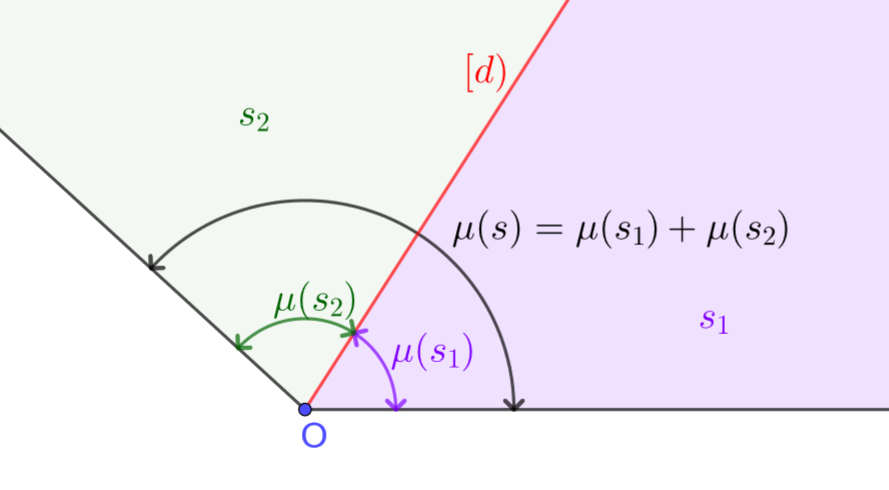
\includegraphics[width=0.7\textwidth]{image/thm_additivite_angles.png}
    \caption{Illustration de la propriété d'additivité des mesures d'angles lorsqu'on sépare un secteur d'angle par une demi-droite $[d)$ (en rouge sur la figure).}
    \label{fig_addi_angles}
\end{figure}
\begin{prop}
    Si deux secteurs d'angles on même mesure alors ils sont congruents.
\begin{scheme}
    On ramène le premier angle dans un des demi-plan du second avec l'isometrie canonique et on raisonne par l'absurde si la demi droite n'est pas envoyer sur l'autre alors on montre a l'aide de la propositions précédentes que les mesure sont différentes. Donc forcement les demi-droites correspondent. La congruance se déduit de la definition de l'application canonique.
\end{scheme}
\end{prop}
\begin{thm}
    Deux secteurs d'angles on même mesure \ssi ils sont congruents. 
\end{thm}

    
    \section{Angles et orientation}

Au collège ou au lycée, la confusion entre angle et secteur d'angle est entretenue par les programmes officiels\,: le même mot \guil{angle} peut désigner un secteur d'angle (un lieu géométrique) ou une mesure d'angle (un nombre). L'égalité entre deux \guil{angles} sous-entendue par les élèves est celle de la mesure d'angle tandis que l'égalité des professeurs (non ignorants) et celles de la classe d'équivalence des secteurs d'angles sous relation d'isométrie. Autrement dit l'élève égalise deux \guil{angles} s'ils ont même mesure alors que le professeurs n'égalise ces \guil{angles} que s'il peut identifier un congruence entre le premier et le second.

Nous avons dans les partie qui précèdent établit un grand nombre de résultat concernant les congruences entre secteurs d'angles. Il est pratique d'introduire alors les classes d'équivalences des secteurs d'angles sous la relation de congruence : l'angle.

        \subsection{Angles}

\begin{defi}[Angles]\label{defi-angle}
    Pour tout secteur d'angle saillant $s$ on appelle angle $\widehat{s}$ la classe d'équivalence de $s$ sous la relation de congruence, autrement dit,
    \begin{equation*}
        \widehat{s} = \ensemble{s' \text{ secteurs d'angles}}{s' \equiv \, s}\,.
    \end{equation*}
    
    Un angle $\mathcal{A}$ est alors un ensemble de secteur d'angle tel qu'il existe un secteur d'angle $s$ tel que $\mathcal{A}=\widehat{s}$. 
\end{defi}

\begin{thm}[Identité de l'angle et de sa mesure]
Pour tout angle $\mathcal{A}$ il existe un unique $\mu_0\in ]0,\pi[$ tel que  pour tout $s \in \mathcal{A}$ on ait $\mu(s)=\mu_0$. $\mu_0$ est alors appelé mesure de l'angle $\mathcal{A}$. On note alors,
\begin{equation*}
    \mu\left(\mathcal{A}\right) = \mu_0\,. 
\end{equation*}
Inversement, pour tout nombre $\mu_0 \in ]0,\pi[$, il existe un unique angle $\mathcal{A}$ tel que $\mu\left(\mathcal{A}\right)=\mu_0$.
\end{thm}
\begin{rema}
    Ce théorème permet d'établir une relation univoque entre les angles et leurs mesures. Ceci justifie qu'on puisse parler indifféremment d'angle et de mesure d'angle. Désormais, donc, on identifie les mesures d'angles avec leurs angles\,: alors pour tout angle $\mathcal{A}$ on note (pas si) abusivement (que ça),
    \begin{equation*}
        \mathcal{A} = \mu \left(\mathcal{A}\right)\,.
    \end{equation*}
\end{rema}

        \subsection{Rotation du plan}

\begin{defi}[Orientations respective des demi-plan orienté de même centre]
On dira que les demi-plans orienté $\overrightarrow{\mathcal{P}}_1 = \left(\mathcal{P}_1,]d_1)\right)$ et $\overrightarrow{\mathcal{P}}_2 = \left(\mathcal{P}_2,]d_2)\right)$ de même centre $O$ sont orienté en même façon \ssi
\begin{equation*}
    \mathcal{P}_1 \cap \mathcal{P}_2 %= s \quad \text{ou}\quad \mathcal{P}_1 \cap \mathcal{P}_2 = \bar{s}\,,
\end{equation*}
est un secteur d'angle saillant complémentaire de $\anglesaillant \left(O,]d_1),]d_2)\right)$. Sinon on dira qu'ils sont orienté différemment.
%où $s = \anglesaillant \left(O,]d_1),]d_2)\right)$ et $\bar{s}$ son secteur d'angle opposée par le sommet. 
\end{defi}
\begin{rema}
    Si $\overrightarrow{\mathcal{P}}_1 = \left(\mathcal{P}_1,]d_1)\right)$ et $\overrightarrow{\mathcal{P}}_2 = \left(\mathcal{P}_2,]d_2)\right)$ sont orienté différemment alors,
\begin{equation*}
    \mathcal{P}_1 \cap \mathcal{P}_2 = s \quad \text{ou}\quad \mathcal{P}_1 \cap \mathcal{P}_2 = \bar{s}\,,
\end{equation*}
où $s = \anglesaillant \left(O,]d_1),]d_2)\right)$ et $\bar{s}$ son secteur d'angle opposée par le sommet. 
\end{rema}
\begin{rema}
    La proposition \ref{prop-existetuniqueopposesommet} assure l'existence et l'unicité de $\bar{s}$
\end{rema}

\begin{prop}[Deux paires de plan orienté en même façon]\label{prop-pairsplanoriente}
    Soit $]d_1)$ et $]d_2)$ deux demi-droites de même extrémité $O$. 
    
    Notons $\mathcal{P}_1$ le demi plan de droite support $(d_1)$ contenant $]d_2)$ et $\bar{\mathcal{P}_1}$ l'autre, $\mathcal{P}_2$ le demi-plan de droite support $(d_2)$ ne contenant pas $]d_1)$ et $\bar{\mathcal{P}_2}$ l'autre.

    Notons $\overrightarrow{\mathcal{P}}_1^+ = (\mathcal{P}_1,]d_1))$, $\overrightarrow{\mathcal{P}}_2^+ = (\mathcal{P}_2,]d_2))$, $\overrightarrow{\mathcal{P}}_1^- = (\bar{\mathcal{P}}_1,]d_1))$ et $\overrightarrow{\mathcal{P}}_2^- = (\bar{\mathcal{P}}_2,]d_2))$ les quatre plan orienté de centre $O$ qu'on peut construire avec les demi-droites $]d_1)$ et $]d_2)$. 

    Alors,
    \begin{itemize}[$\bullet$]
        \item $\overrightarrow{\mathcal{P}}_1^+$ et $\overrightarrow{\mathcal{P}}_2^+$ sont orienté en même façon,
        \item $\overrightarrow{\mathcal{P}}_1^-$ et $\overrightarrow{\mathcal{P}}_2^-$ sont orienté en même façon,
        \item tandis que $\overrightarrow{\mathcal{P}}_1^+$ et $\overrightarrow{\mathcal{P}}_2^-$ sont orienté différemment,
        \item $\overrightarrow{\mathcal{P}}_1^-$ et $\overrightarrow{\mathcal{P}}_2^+$ sont orienté différemment.
    \end{itemize}
\end{prop}

\begin{defi}[Rotation]
    Soit $]d_1)$ et $]d_2)$ deux demi-droite d'extrémité $O$. On reprend alors les notations de la proposition \ref{prop-pairsplanoriente}. On note également $]\bar{d_1})$ (respectivement $]\bar{d_2})$) la demi-droite ouverte supplémentaire de $]d_1)$ (respectivement $]d_2)$). 

    La rotation $R_{]d_1),]d_2)}$ envoyant $]d_1)$ sur $]d_2)$ est une application $R_{]d_1),]d_2)} : \mathcal{E} \to \mathcal{E}$ définie comme suit :
    \begin{equation*}
        \begin{array}{ccccc}
        R_{]d_1),]d_2)} & : &  \mathcal{E} & \to &  \mathcal{E} \\
         & & O & \mapsto & O \\
         & & M\in ]d_1) & \mapsto & M' \text{ le report de } [OM] \text{ sur } ]d_2) \\
         & & M\in ]\bar{d_1}) & \mapsto & M' \text{ le report de } [OM] \text{ sur } ]\bar{d_2}) \\
        & & M\in \mathcal{P}_1^+ & \mapsto & \mathcal{I}_{\overrightarrow{\mathcal{P}}_1^+,\overrightarrow{\mathcal{P}}_2^+} (M) \\
        & & M\in  \mathcal{P}_1^- & \mapsto & \mathcal{I}_{\overrightarrow{\mathcal{P}}_1^-,\overrightarrow{\mathcal{P}}_2^-} (M) \\
        \end{array}\,.
    \end{equation*}
\end{defi}
\begin{thm}
    Soit $]d_1)$ et $]d_2)$ deux demi-droite d'extrémité $O$ alors la rotation $R_{]d_1),]d_2)}$ envoyant $]d_1)$ sur $]d_2)$ est une Isométrie. 
\end{thm}

        \subsection{Translation}

\begin{defi}[Translation]
    Soit $A$ et $B$ deux points, on appelle translation amenant $A$ sur $B$ l'application du plan $\tau_{\vb{AB}} : \mathcal{E} \to \mathcal{E}$ qui :
    \begin{itemize}[$\bullet$]
        \item à tout point $M$ en dehors de $(AB)$ associe l'unique point $M'$ intersection de l'unique parallèle à $(AB)$ passant par $M$ et de l'unique parallèle à $(AM)$ passant par $B$. 
        \item à tout point de $]AB)$ associe l'unique point $M'$ tel que $A\star M \star M'$ et $[AB]\equiv [MM']$
        \item à tout point de $(AB)-[AD)$ associe l'unique point $M'$ tel que $M\star M' \star B$ et $[AB]\equiv [MM']$
        \item à $A$ associe $B$.
    \end{itemize}
\end{defi}  
\begin{rema}
    L'axiome des parallèles \ref{axi-parra} assure l'univocité de cette application.
\end{rema}
\begin{thm}
    Soit $A$ et $B$ deux points alors $\tau_{\vb{AB}}$ la translation envoyant $A$ sur $B$ est une isométrie. 
\end{thm}

        \subsection{Inégalité triangulaire et conséquences}

Afin d'établir quelques propriétés essentiels des isométries qui nous servirons dans notre construction de la notion d'angle orienté, nous avons besoin d'un résultat essentiel : l'inégalité triangulaire. Celle-ci repose sur un série de Lemme:

%\begin{prop}\label{prop-rajlong}
%    Soit $A,B$ et $C$ trois points alors $AB \leq AB + BC$.
%\end{prop}

\begin{thm}[Théorème de l'angle extérieur]
    Soit $A,B$ et $C$ trois points distinct, alors dans le triangle $ABC$ la mesure de l'angle supplémentaire en $A$ est supérieur à l'angle en $A$ où en $B$.
% 4.12 dans le document pour les profs :https://publimath.univ-irem.fr/numerisation/LY/ILY98002/ILY98002.pdf
\end{thm}

\begin{lem}
Dans un triangle, si deux cotés n'ont pas même mesure alors les angles des sommets opposés aux cotés correspondant sont également de mesure différentes. De plus au coté le plus long est opposé le secteur d'angle de plus grande mesure. 
\end{lem}
\begin{lem}\label{lem-i3}
Dans un triangle, si deux angles au sommets sont de mesure différentes alors les cotés opposés au angles sommet correspondant sont également de mesure différentes. De plus à l'angle au sommet de plus grande mesure est opposée le cotés de plus grande mesure.  
\end{lem}


\begin{thm}
Soit $A,B$ et $C$ trois points, alors,
\begin{equation*}
AB \leq AC + CD
\end{equation*}
où l'égalité est réalisé uniquement si $C\in [AB]$,
\begin{equation*}
    AB = AC + AD \quad \Longleftrightarrow \quad C\in [AB] 
\end{equation*}

\begin{proof}
On commence avec le cas de trois points $A,B$ et $C$ non-alignés (distinct et tel que $C\notin (AB)$). 

Notons $[d)$ la demi-droite fermé supplémentaire de la demi-droite ouverte $]CB)$ et notons (Axiome \ref{axi-C1}) l'unique point $D \in [d)$ tel que $CA\equiv CD$.  

Par construction on a $B\star C \star D$ en effet les trois points appartenant à la même droite $(BC)$ respectent un alignement à trois points parmi trois possible (Axiome \ref{ax-B3}). Les deux autres possibles sont exclus du fait que $D \notin ]CB)$. 

Ainsi, $C \in ]DC[$ et donc (Prop. \ref{prop-barrtrans}) $C\in \anglesaillant \left( A,]AB),])AD)\right)$. Puis, en vertu de (Prop. \ref{thm-incluspart}) on a,
\begin{equation*}
\anglesaillant \left( A,]AC),])AD)\right)\varsubsetneq \anglesaillant \left( A,]AB),])AD)\right)
\end{equation*}
et par suite,
\begin{equation*}
\anglesaillant \left( A,]AC),])AD)\right) < \anglesaillant \left( A,]AB),])AD)\right)\,.
\end{equation*}  

Or par construction $ACD$ est isocèle en $C$ et $]DC)=]DB)$ (car $C\in]BC[$) donc (Prop. \ref{prop-isocelecongruenceangle}),
 \begin{align*}
\anglesaillant \left( D,]DA),])DB)\right) \equiv \anglesaillant \left( D,]DA),])DC)\right)  \equiv \anglesaillant \left( A,]AC),])AD)\right) 
\end{align*}
et par compatibilité de la congruence avec relation d'ordre sur le secteurs d'angle,
\begin{equation*}
    \anglesaillant \left( D,]DA),])DB)\right) < \anglesaillant \left( A,]AB),])AD)\right)\,.
\end{equation*}

En utilisant le Lemme \ref{lem-i3} dans le triangle $ABD$ (qui est non aplatit car sinon cela voudrai dire que $A\in (BD)=(BC)$ et on a pris $A,B$ et $C$ non alignés) et sur les angles au sommets $A$ et $D$ que,
\begin{equation*}
AB<BD
\end{equation*}
or puisque $C\in ]BD[$ on peut utiliser la proposition \ref{prop-addlong} pour déduire que $BD=BC+CD$, enfin puisque $CD=AC$ on a,
\begin{equation*}
AB < AC + CB\,.
\end{equation*}

Dans le cas ou les points $A,B$ ou $C$ sont alignés il y a trois cas à considérer : 
\begin{itemize}[$\bullet$]
\item soit $A\star C \star B$ on  a $C \in ]AB[$ et donc (Prop. \ref{prop-addlong}) $AB = AC + CB$,
\item soit $C\star A \star B$ alors $A\in ]CB[$ et donc (définitions \ref{def-ineqlong}) $AB < BC$.  Ce qui (Prop. \ref{prop-addlong}) implique $AB < BC \leq AC + CB $. Ainsi, $ AB < AC + CB$.
\item soit  $A\star B \star C$, alors $B\in ]CA[$ et donc (définitions \ref{def-ineqlong}) $AB < AC$. De même (Prop. \ref{prop-addlong}) $AB < AC \leq AC + CB$. 
\end{itemize}
\end{proof}
\end{thm}

\begin{cor}
    L'image d'une droite (demi-droite, segment) par une isométrie est une droite (demi-droite, segment). 
\end{cor}

        \subsection{Secteur d'angle orienté}

\begin{defi}[Secteurs d'angles orienté]
    On appelle secteurs d'angles orienté les couples de demi-droite $o = \left(]d_1),]d_2)\right)$ de même extrémité. L'extrémité commune des demi-droite est appelé sommet de $o$.
\end{defi}
\begin{rema}
    Pour tout secteurs d'angle orienté $o = \left(]d_1),]d_2)\right)$ de sommet $O$, on notera $\anglesaillant o = \anglesaillant \left(]d_1),]d_2)\right)= \anglesaillant\left(O,]d_1),]d_2)\right)$.
\end{rema}
\begin{defi}[Plan orienté associé à un angle orienté]
    Pour tout secteur d'angle orienté $\left(]d_1),]d_2)\right)$ on appelle demi-plan orienté associé le plan orienté $\overrightarrow{\mathcal{P}}=\left(\mathcal{P}_{(d_1),]d_2)},]d_1)\right)$.
\end{defi}
\begin{defi}[Orientation respective des secteurs d'angles orientés]
    Deux secteurs d'angles orienté sont orienté en même façon \ssi leurs demi-plan orienté associé le sont. On dit qu'ils sont orienté différemment sinon. 
\end{defi}
\begin{prop}
    La relation d'orientation respective entre secteurs d'angle orienté est une relation d'équivalence.
\end{prop}
\begin{defi}[Plan orienté]
L'espace euclidien $\mathcal{E}$ est dit orienté \ssi il est muni d'un secteurs d'angle orienté $r = \left(]d_I),]d_J)\right)$. On note $(\mathcal{E},r)$ l'espace euclidien orienté définit.
\end{defi}
\begin{defi}[Orientation]
Dans un plan euclidien orienté $(\mathcal{E},r)$ on dit que le secteur d'angle orienté $\left(]d_1),]d_2)\right)$ est orienté positivement \ssi $r$ et $\left(]d_1),]d_2)\right)$ sont orienté en même façon. Sinon on dira que l'angle orienté $\left(]d_1),]d_2)\right)$ est orienté negativement.
\end{defi}

        \subsection{Angle orienté}

\begin{defi}[Congruence entre angle orienté]
Soit $o_1$ et $o_2$ deux secteurs d'angle orienté on dira que ces secteurs d'angles sont congruents \ssi $o_1$ et $o_2$ sont orienté en même façon et que $\anglesaillant o_1$ et $\anglesaillant o_2$ sont congruent. 

On notera également $\equiv$ cette relation.
\end{defi}
\begin{prop}
    La relation de congruence entre secteurs d'angle orienté est une relation d'équivalence.
\end{prop}
\begin{defi}[Angle orienté]
    Pour tout secteur d'angle orienté $o$ on appelle angle orienté $\widehat{o}$ de représentant $o$ la classe d'équivalence de $o$ sous la relation de congruence entre angle orienté, autrement dit,
    \begin{equation*}
        \widehat{o} = \ensemble{o' \text{ secteurs d'angles orienté}}{o' \equiv \, o}\,.
    \end{equation*}
    
    Un angle orienté $\mathcal{O}$ est alors un ensemble de secteur d'angle orienté tel qu'il existe un secteur d'angle orienté $o$ tel que $\mathcal{O}=\widehat{o}$. 
\end{defi}

        \subsection{Mesure des secteurs d'angles orientés}

\begin{defi}[Mesure d'un angle orienté]
    Dans un plan euclidien orienté $(\mathcal{E},r)$ la mesure du secteurs d'angle orienté $o$ est,
    \begin{equation*}
        \mu(o) = \pm \mu\left(\anglesaillant o\right)
    \end{equation*}*
    où $\pm = +$ si $r$ et $o$ sont orienté en même façon et $\pm = -$ sinon.
\end{defi}
\begin{thm}
    Soit $\mathcal{O}$ un angle orienté, alors il existe $\mu_0\in ]-\pi,\pi[$ tel que pour tout $o\in \mathcal{O}$ on a $\mu(o)=\mu_0$. On appellera alors mesure de $\mathcal{O}$ le nombre $\mu_0$. On note alors $\mu\left(\mathcal{O}\right)$ la mesure de l'angle orienté $\mathcal{O}$.  
\end{thm}
% reciproque


\chapter{Trigonométrie circulaire}\label{chap_fcttrigo}

\section{Fonctions trigonométriques}
	

	\subsection{Sinus et cosinus}\label{subsec_sincos}
		\begin{defi}[Cercle trigonométrique]
			Soit $(O,I,J)$ un repère orthonormé direct. On définit le cercle trigonométrique $\S$ comme étant le cercle de centre $O$ et de rayon $1$.
		\end{defi}
		\paragraph{Remarques.} 

		\begin{enumerate}
			\item Usuellement, dans les livres de mathématiques, on note $\S_1$ le cercle de rayon 1, $\S_2$ la sphère de rayon 1, $S_3$ l'hypersphère de rayon 1. Les nombres des indices correspondent aux dimensions des objets\,: le cercle $\S_1$ est un objet de dimension 1, la sphère $\S_2$ est un objet de dimension 2, l'hypersphère $\S_3$ est un objet de dimension 3, etc. Comme il ne sera que question de $\S_1$ ici, afin d'alléger les notations, on note par convention $\S=\S_1$.
		
			\item Si l'on se donne plusieurs repères orthonormés du plan, alors on peut envisager plusieurs cercles trigonométriques dans le plan.
		\end{enumerate}

		\begin{defi}[Cosinus et sinus]
			Soit $\S$ le cercle trigonométrique de centre $O$. Soit $(O;I;J)$ un repère orthonormé direct unitaire. On note $\S^+$ le demi-cercle obtenu par l'intersection de $\S$ et du demi-plan fermé d'extrémité $(OI)$ et qui contient $J$. On note $\S^-$ le demi-cercle obtenu par l'intersection de $\S$ et du demi-plan ouvert d'extrémité $(OI)$ qui ne contient pas $J$, à savoir $\S^-=\S-(\S^+-(OI))$ (voir figure \ref{fig_def_trigo_Spm}). 

			Soit $M\in\S^+$. Alors $\widehat{IOM}$ est un angle saillant dont la mesure est la longueur de l'arc $\wideparen{IM}$. Le point $M$ est déterminé par la mesure de l'angle $\widehat{IOM}$. Ses coordonnées sont donc des fonctions de cet angle. 
			Lorsque $M\in\S^-$, $\widecheck{IOM}$ est un angle rentrant dont la mesure est $2\pi$ moins la longueur de l'arc $\wideparen{IM}$. (Voir figure \ref{fig_def_trigo_Spm})

			Dans les conditions énoncées ci-dessus, on aura deux cas possibles\,:
			\begin{enumerate}
			 	\item Si $M\in\S^+$\,:
 				\begin{itemize}[label=\textbullet]
					\item on appelle cosinus de l'angle $\widehat{IOM}$, et on note $\cos\widehat{IOM}$, l'abscisse du point $M$,
					\item on appelle sinus de l'angle $\widehat{IOM}$, et on note $\sin\widehat{IOM}$, l'ordonnée du point $M$.
				\end{itemize}
				\item Si $M\in\S^--(OI)$\,:
				\begin{itemize}[label=\textbullet]
					\item on appelle cosinus de l'angle $\widecheck{IOM}$, et on note $\cos\widecheck{IOM}$, l'abscisse du point $M$,
					\item on appelle sinus de l'angle $\widecheck{IOM}$, et on note $\sin\widecheck{IOM}$, l'ordonnée du point $M$.
				\end{itemize}
			 \end{enumerate} 
			Autrement dit\,: 
			\begin{equation}
				M(x,y)\in\S^+ \Leftrightarrow \(\cos\widehat{IOM}=x \wedge \sin\widehat{IOM}=y\).
			\end{equation}
			\begin{equation}
				M(x,y)\in\S^- \Leftrightarrow \(\cos\widecheck{IOM}=x \wedge \sin\widecheck{IOM}=y\).				
			\end{equation}
		\end{defi}

		\begin{figure}
			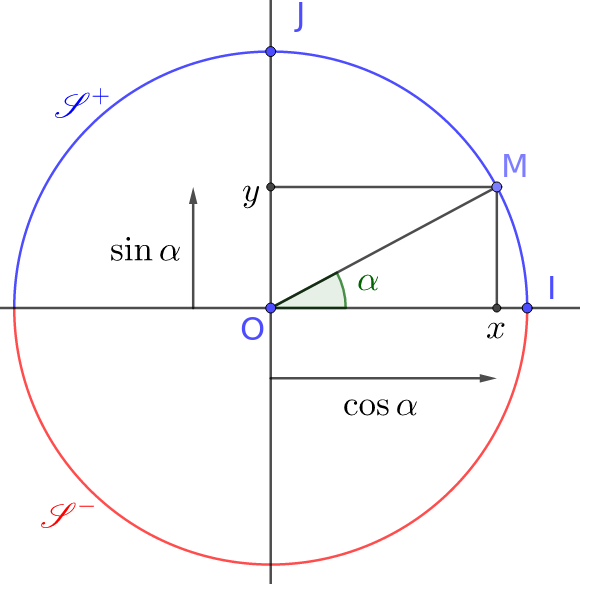
\includegraphics[width=0.46\textwidth]{image/fct_trigo/def_trigo_sp.png}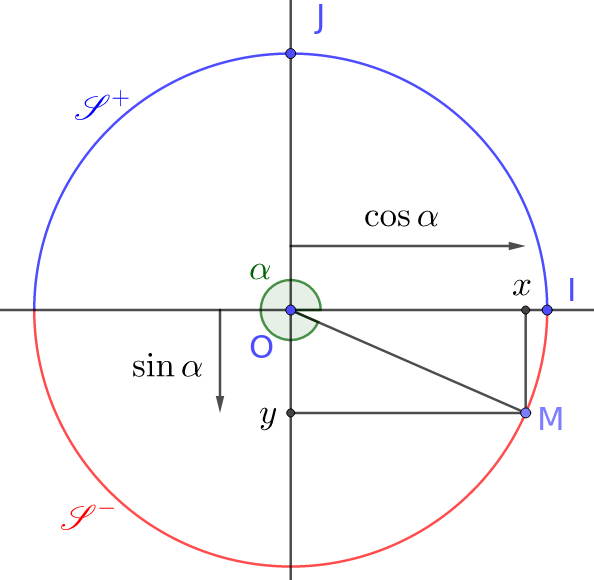
\includegraphics[width=0.46\textwidth]{image/fct_trigo/def_trigo_sm.png}
			\caption{À gauche\,: définition des fonctions trigonométriques dans le cas où $M\in\S^+$. À droite\,: idem, dans le cas où $M\in\S^-$.}
			\label{fig_def_trigo_Spm}
		\end{figure}

		\paragraph{Remarque.} Cette définition est un peu lourde, et on peut avantageusement la simplifier en considérant un angle orienté $\alpha=\ovr{(O,I,M)}$ qui vérifie $-\pi<\alpha\le \pi$. En effet, si l'on part du point $I$ et que l'on effectue une rotation orientée de centre $O$ et d'angle $\alpha$ avec $-\pi<\alpha<0$, le résultat de cette rotation se situera sur $\S^--(OI)$ et on sera dans le point 2 de la définition\,; si $0\le\alpha\le\pi$, on se situe dans $\S^+$ et dans ce cas on est dans le point 1 de la définition. On peut donc avantageusement récrire cette définition\,:

		\begin{defi}[Cosinus et sinus orientés]
			Soit $M\in\S$. Alors il existe un unique nombre réel $\alpha\in]-\pi,\pi]$ tel que $M$ soit l'image de la rotation de centre $O$ et d'angle orienté $\alpha$. $M$ ayant pour coordonnées $(x,y)$, on pose par convention
			\begin{equation}
				\cos\alpha = x,\quad \sin\alpha = y.
			\end{equation}
		\end{defi}

		\begin{figure}
			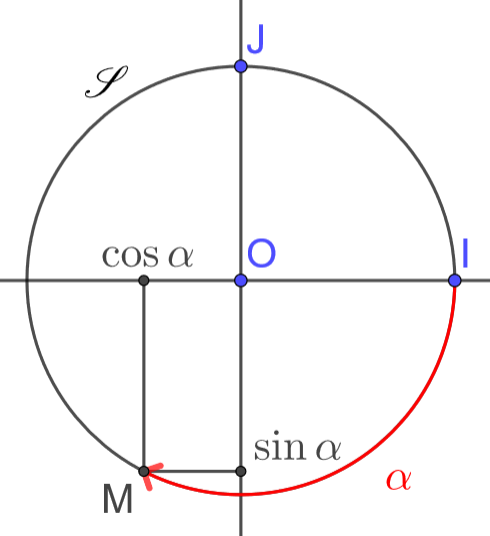
\includegraphics[width=0.37\textwidth]{image/fct_trigo/cossin_oriente_m.png}\hspace{0.1cm}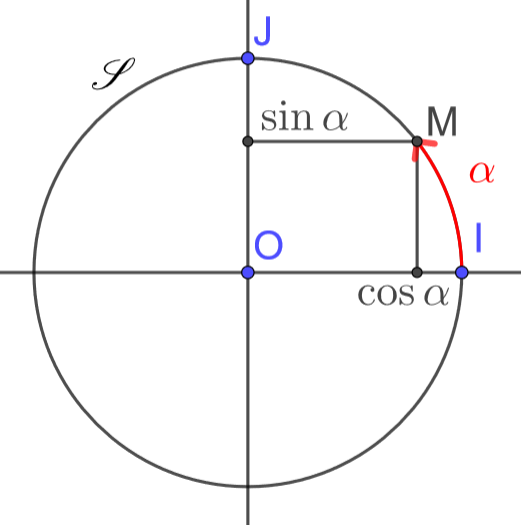
\includegraphics[width=0.4\textwidth]{image/fct_trigo/cossin_oriente_p.png}
			\caption{Illustration de la définition des fonctions trigonométriques dans le cas des angles orientés. À gauche, $-\pi<\alpha<-\frac{\pi}{2}$. Dans ce cas, $\cos\alpha<0$ et $\sin\alpha<0$. À droite, $0<\alpha<\frac{\pi}{2}$. Dans ce cas, $\cos\alpha>0$ et $\sin\alpha>0$.}
		\end{figure}

		\paragraph{Remarque.} On peut en fait définir les fonctions trigonométriques sur tout intervalle de la forme $]x,x+2\pi]$, ou $[x,x+2\pi[$, si l'on souhaite parcourir le cercle trigonométrique une seule fois et avoir une relation univoque entre l'angle et la position du point sur le cercle. Certains livres définissent les fonctions trigonométriques sur $[0,2\pi[$.

		\vspace{0.3cm}

		Il est également possible de définir les fonctions trigonométriques sur $\R$ en ramenant tout nombre réel à un nombre de l'intervalle $]-\pi,\pi]$. En effet, en vertu de la propriété archimédienne de $\R$, pour tout nombre réel $r$, il existe un entier relatif $k$ tel que $(2k-1)\pi<r\le (2k+1)\pi$. Dans ce cas, on dit que le nombre $r$ est congru à $r'=r-2k\pi$ modulo $2\pi$\,; alors $r'\in]-\pi,\pi]$. En fait, dire que $r$ et $r'$ sont congrus modulo $2\pi$ revient à dire que les rotations d'angles $r$ et $r'$ sont identiques à $k$ tours complets près (voir figure \ref{fig_congr}). Formellement, on a la définition suivante\,:
		\begin{defi}[Congruence modulo $2\pi$]
			Soient $u,v\in\R$. $u$ et $v$ sont congrus modulo $2\pi$ signifie qu'il existe un entier relatif $k$ tel que $u=v+2k\pi$. Formellement\,:
			\begin{equation}
				u\equiv v [2\pi] \Leftrightarrow \exists k\in\Z, u=v+2k\pi.
			\end{equation}
		\end{defi}

		\begin{figure}
			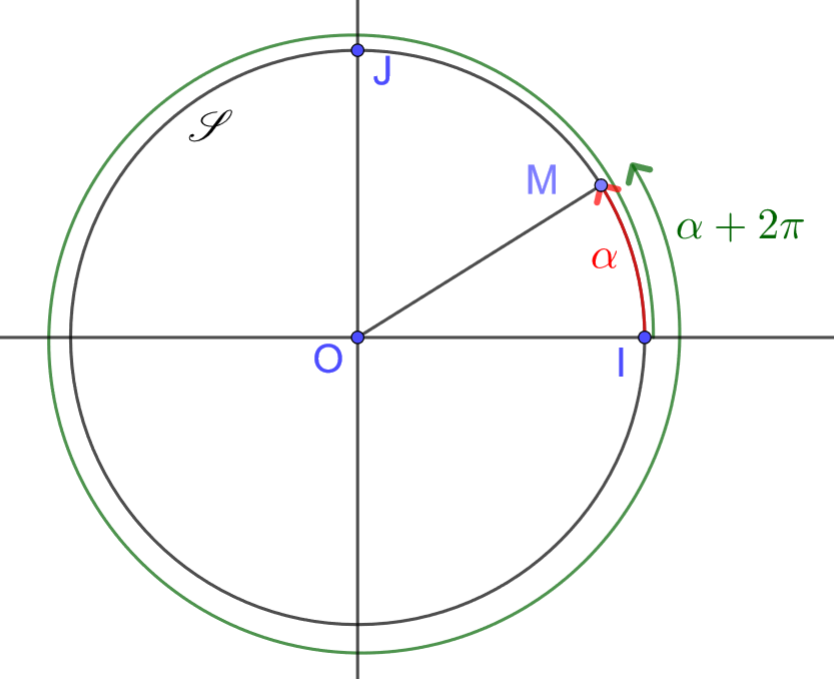
\includegraphics[width=0.5\textwidth]{image/fct_trigo/congr.png}
			\caption{Illustration de la congruence modulo $2\pi$\,: on voit que les $\alpha$ et $\alpha+2\pi$ correspondent au même point sur le cercle trigonométrique, puisque l'angle $2\pi$ correspond à un tour complet.}
			\label{fig_congr}
		\end{figure}

		\paragraph{Remarque.} L'extension de la congruence modulo n'importe quel nombre est triviale.


		Ainsi, en se ramenant à des valeurs comprises entre $-\pi$ et $\pi$, on peut prolonger les fonctions cosinus et sinus au delà de leur intervalle de définition initial. Cela nous donne donc la définition suivante\,:

		\begin{defi}[Cosinus et sinus sur $\R$]
			Soit $u$ un nombre réel. Alors il existe un unique nombre réel $v$ tel que $(u\equiv v\mod[2\pi])\wedge(-\pi<v\le\pi)$, et dans ce cas, on pose
			\begin{equation}
				\cos u= \cos v,\quad \sin u=\sin v.
			\end{equation}
		\end{defi}

		\paragraph{Explication visuelle.} Si l'on souhaite calculer le cosinus et le sinus d'un angle $u$, où $u\notin]-\pi,\pi]$, géométriquement, ramener $u$ à un angle compris entre $-\pi$ et $\pi$ revient à \guil{enrouler} un segment de longueur $u$ autour du cercle trigonométrique et regarder où se situe l'extrémité du segment\footnote{C'est cette idée que nous avons représentée dans la figure \ref{fig_congr}, mais une animation geogebra montre explicitement cet \guil{enroulement}\,: \url{https://www.geogebra.org/m/Ry4j9ZT2}}. 

	\subsection{Tangente}
		\begin{defi}
			Soit $M\in\S-(J\cup J')$ où $J'$ est diamétralement opposé à $J$ sur $\S$. Soit $(d)$ la perpendiculaire à $(OI)$ passant par $I$. Soit $N=(OM)\cap(d)$ (Voir figure \ref{fig_tangente}). Alors on définit la tangente de l'angle orienté $\alpha=\ovr{(O,I,M)}$\,:
			\begin{itemize}[label=\textbullet]
				\item Si $N$ est du même côté que $\S^+$ de $(OI)$, $\tan\alpha=IN$,
				\item Sinon, $\tan\alpha=-IN$.
			\end{itemize}
		\end{defi}

		\begin{figure}
			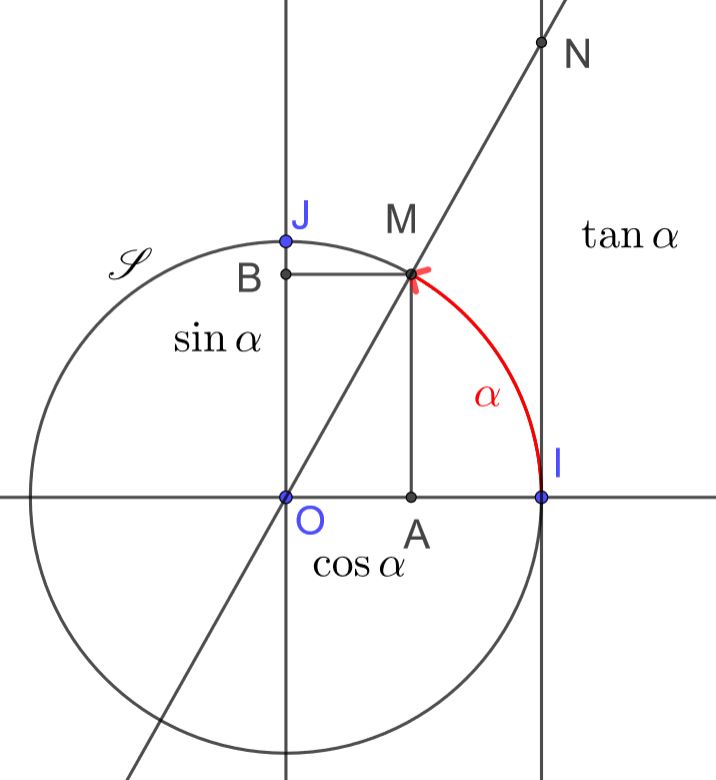
\includegraphics[width=0.4\textwidth]{image/fct_trigo/tangente.png}
			\caption{Construction géométrique de la tangente. Ici, $0<\alpha<\frac{\pi}{2}$, $OA=\cos\alpha$, $OB=BM=\sin\alpha$, $IN=\tan\alpha$.}
			\label{fig_tangente}
		\end{figure}

		\paragraph{Remarque.} De même que pour les fonctions cosinus et sinus, la définition de la fonction tangente s'étend sur $\R-\left\{\frac{\pi}{2}+k\Z\right\}$.

		\begin{thm}
			\begin{equation}
				\forall \alpha\in\R-\left\{\frac{\pi}{2}+k\Z\right\}, \tan\alpha=\frac{\sin\alpha}{\cos\alpha}.
			\end{equation}
		\end{thm}

		\begin{proof}
			On démontre le théorème dans le cas où $\alpha\in\[\left.0,\frac{\pi}{2}\right[\right.$, on laisse les autres cas au lecteur.
			Considérons la figure $\ref{fig_tangente}$. Par construction, $(IN)\sslash (AM)$, et on a $O\star A\star I$ et $O\star M\star N$. D'après le théorème de Thalès, on a 
			\begin{equation}
				\frac{IN}{AM}=\frac{OI}{OA} \label{eq_thales_trigo}
			\end{equation}
			Mais $IN=\tan\alpha$, $OI=1$, $OA=\cos\alpha$ et $AM=\sin\alpha$. Donc
			\begin{equation}
				\eqref{eq_thales_trigo}\Leftrightarrow \frac{\tan\alpha}{\sin\alpha}=\frac{1}{\cos\alpha}\Leftrightarrow\tan\alpha=\frac{\sin\alpha}{\cos\alpha}.
			\end{equation}
		\end{proof}

	\subsection{Exercices}
		\paragraph{Exercice 1.}
			Soit $\S$ le cercle trigonométrique dans un repère orthonormé direct $(O,I,J)$.
			\begin{enumerate}[1)]
				\item Placer un point $M$ sur $\S$, de coordonnées $(x,y)$, tel que $y=\frac{1}{2}$, et $x>0$. Combien vaut $\sin\widehat{IOM}$\,?
				\item Calculer $\cos\widehat{IOM}$. Calculer $\tan\widehat{IOM}$.
				\item Placer $N\in\S$, de coordonnées $(x',y')$, tel que $x'=\frac{1}{2}$ et $y'>0$.
				\item Remarquer une symétrie, et sans aucun calcul, en déduire les valeurs de $\cos\widehat{ION}$ et $\sin\widehat{ION}$.
			\end{enumerate}

		\paragraph{Exercice 2.}
			\begin{enumerate}[1)]
				\item Démontrer que $\forall x\in\R$, $\cos^2x+\sin^2x=1$.
				\item Soit $x\in\R$. Calculer les nombres suivants en fonction de $\cos x$ et $\sin x$\,:
				\begin{equation}
					\cos(-x);\quad \sin(-x);\quad \cos(\pi+x);\quad \sin(\pi+x);\quad \cos(\pi-x);\quad \sin(\pi-x); \nonumber
				\end{equation}
				\begin{equation}
					\quad\cos\(\frac{\pi}{2}+x\);\quad\sin\(\frac{\pi}{2}+x\);\quad\cos\(\frac{\pi}{2}-x\);\quad\sin\(\frac{\pi}{2}-x\);\quad\nonumber
				\end{equation}
				On pourra s'aider avantageusement d'un schéma du cercle trigonométrique et de considérations sur des symétries axiales et rotatives.
			\end{enumerate}


	\subsection{Trigonométrie dans le triangle rectangle}

		Dans tout triangle rectangle, les angles aux sommets sont compris entre 0 et $\frac{\pi}{2}$ et peuvent être considérés comme non orientés. 

		\begin{thm}
			Soit un triangle $ABC$ rectangle en $B$. Soit $\alpha=\widehat{BAC}$. Alors\,:
			\begin{equation}
				\cos\alpha=\frac{AB}{AC},
			\end{equation}
			\begin{equation}
				\sin\alpha=\frac{BC}{AC},
			\end{equation}
			\begin{equation}
				\tan\alpha=\frac{BC}{AB}.
			\end{equation}
			Par rapport au sommet $A$, on peut nommer les côtés\,: $[AC]$ étant l'hypothénuse du triangle rectangle, $[AB]$ est le côté adjacent (au sommet $A$), tandis que $[BC]$ est le côté opposé (au sommet $A$). On peut donc reformuler le théorème de manière \guil{mnémotechnique}\,:
			\begin{equation}
				\cos\alpha=\frac{\text{mesure du côté adjacent}}{\text{mesure de l'hypothénuse}}
			\end{equation}
			\begin{equation}
				\sin\alpha=\frac{\text{mesure du côté opposé}}{\text{mesure de l'hypothénuse}}
			\end{equation}
			\begin{equation}
				\tan\alpha=\frac{\text{mesure du côté opposé}}{\text{mesure du côté adjacent}}.
			\end{equation}
		\end{thm}

		\begin{figure}
			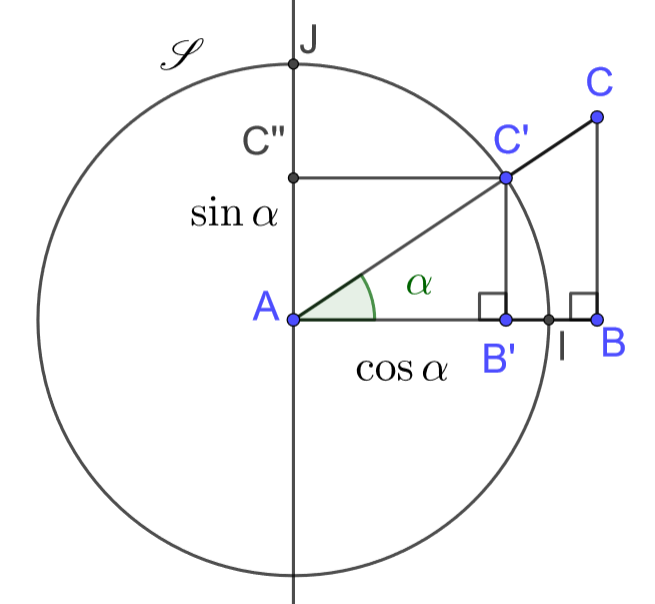
\includegraphics[width=0.4\textwidth]{image/fct_trigo/trigo_triangle.png}
			\caption{Figure pour passer d'un triangle rectangle au cercle trigonométrique. On a pris le cas où $AC>1$.}
			\label{fig_trigo_triangle}
		\end{figure}

		\begin{proof}
			On suppose que $\ovr{(A,B,C)}>0$ (le cas contraire se démontre de manière similaire, on laisse donc cela au lecteur). Construisons un cercle trigonométrique $\S$ de centre $A$, et posons $I=(AB)\cap\S$, et soit $J$ tel que $(A,I,J)$ soit un repère orthnormé direct. Soit $C'=(AC)\cup\S$. Soient $B'$ et $C''$ respectivement les projetés orthogonaux de $M$ sur $(OI)$ et sur $(OJ)$ (voir figure \ref{fig_trigo_triangle}). Alors $AB'=\cos\alpha$ et $B'C'=\sin\alpha$. Si $AC=1$, alors $C'=C$, $B'=B$, $BC=B'C'$ et les relations annoncées du théorème sont immédiatement vérifiées. Supposons que $AC>1$. Alors $A\star B'\star B$ et $A\star C'\star C$ (dans le cas contraire, on aurait $A\star B\star B'$ et $A\star C\star C'$). D'après le théorème de Thalès --- et ce, que $AC>1$ ou que $AC<1$ --- on a\,:
			\begin{equation}
				\frac{AB'}{AB}=\frac{AC'}{AC}=\frac{BC'}{BC}. \label{eq_thales_trigotriangle}
			\end{equation} 
			Mais dans le cercle trigonométrique, $\cos\alpha=AB'$, $AC'=1$ et $\sin\alpha=B'C'$. Ainsi, d'après \eqref{eq_thales_trigotriangle},
			\begin{equation}
				\frac{\cos\alpha}{AB}=\frac{1}{AC},\quad \text{donc}\quad \cos\alpha=\frac{AB}{AC}.
			\end{equation}
			De même, d'après \eqref{eq_thales_trigotriangle},
			\begin{equation}
				\frac{\sin\alpha}{BC}=\frac{1}{AC}\quad \text{donc}\quad \sin\alpha=\frac{BC}{AC}.
			\end{equation}
			Enfin,
			\begin{equation}
				\tan\alpha=\frac{\sin\alpha}{\cos\alpha}=\frac{\frac{AB}{AC}}{\frac{BC}{AC}}=\frac{AB}{AC}\cdot\frac{AC}{BC}=\frac{AB}{BC}.
			\end{equation}
		\end{proof}

		\paragraph{Exercice 1} Considérons un triangle $ABC$ rectangle en $B$, avec $AB=3$, $BC=4$.
		\begin{enumerate}[1)]
			\item Calculer $AC$.
			\item On pose $\alpha=\widehat{CAB}$, $\beta=\widehat{ABC}$. Calculer $\cos\alpha$, $\sin\alpha$, $\tan\alpha$. En déduire $\cos\beta$, $\sin\beta$, $\tan\beta$.
		\end{enumerate}

		\paragraph{Exercice 2} 		Aujourd'hui, les programmes de calculs (par exemple dans les calculatrices) permettent de calculer les valeurs des fonctions trigonométriques, des angles étant donnés. En attendant de voir comment les calculer, nous allons utiliser ces valeurs pour calculer des distances.
		
		Considérons un triangle $DEF$ rectangle en $E$ avec $DE=3$, et $\alpha=\widehat{FDE}=\frac{\pi}{6}$.
		\begin{enumerate}[1)]
			\item Utiliser une machine à calculer pour estimer numériquement la valeur de $\tan\(\frac{\pi}{6}\)$.
			\item Exprimer $\tan\alpha$ en fonction de $DF$ et $FE$.
			\item En déduire la valeur exacte, puis approchée, de la distance $FE$.
			\item En procédant de même avec l'aide de la fonction $\cos$, sans utiliser le théorème de Pythagore, calculer la distance $DE$.
		\end{enumerate}

		\paragraph{Exercice 3} Valeurs trigonométriques remarquables.
			Nous allons voir comment calculer certaines valeurs des fonctions trigonométriques (notamment $\pi/6$ utilisée précédemment).
			\begin{enumerate}[1)]
				\item $\pi/3$ et $\pi/6$. On considère un triangle équilatéral $ABC$. Pour simplifier, on prendra $AB=1$.
				\begin{enumerate}[a)]
					\item Justifier que $\widehat{CAB}=\pi/3$.
					\item Soit $H\in(AC)$ tel que $(BH)$ soit un axe de symétrie de la figure. Calculer $AH$ et $\widehat{HBA}$.
					\item Calculer $HB$.
					\item En considérant les bons angles, calculer exactement\,:
					\begin{equation}
						\cos{\frac{\pi}{6}},\quad \sin\frac{\pi}{6},\quad \cos{\frac{\pi}{3}},\quad \sin\frac{\pi}{3},\quad \tan{\frac{\pi}{6}},\quad \tan\frac{\pi}{3}.\nonumber
					\end{equation}
					Si besoin, vérifier les valeurs approchées avec une machine à calculer.
				\end{enumerate}
				\item $\pi/4$. Soit $DEF$ un triangle rectangle isocèle en $E$. Pour simplifier, on prendra $DF=1$.
				\begin{enumerate}[a)]
					\item Justifier que $\widehat{EDF}=\widehat{DFE}=\frac{\pi}{4}$.
					\item Démontrer que $\cos\frac{\pi}{4}=\sin\frac{\pi}{4}$. Calculer ces valeurs.
					\item Calculer $\tan\frac{\pi}{4}$.
					\item Si besoin, tout vérifier à la calculatrice.
				\end{enumerate}
			\end{enumerate}

			\emph{Solution : on peut résumer quelques valeurs particulières des fonctions trigonométriques dans le tableau suivant\,:}

			\renewcommand*{\arraystretch}{1.4}
			\begin{tabular}{cccccc}
				$\alpha$     & 0 & $\frac{\pi}{6}$     & $\frac{\pi}{4}$      & $\frac{\pi}{3}$      & $\frac{\pi}{2}$ \\
				\hline
				$\sin\alpha$ & 0 & $\frac{1}{2}$       & $\frac{\sqrt{2}}{2}$ & $\frac{\sqrt{3}}{2}$ & 1 \\
				$\cos\alpha$ & 1 & $\frac{\sqrt{3}}{2}$& $\frac{\sqrt{2}}{2}$ & $\frac{1}{2}$        & 0 \\
				$\tan\alpha$ & 0 & $\frac{\sqrt{3}}{3}$& 1                    & $\sqrt{3}$           & non défini
			\end{tabular}

		\paragraph{Exercice 4} (Géométrie sphérique sur la Terre)

			La surface de la Terre est modélisée par une sphère de rayon $R=CE=CM=CN=CS\approx 6400$km. Les \emph{parallèles} sont des cercles inscrits sur la sphère, perpendiculaires à l'axe Nord-Sud $(NS)$. L'équateur est le parallèle qui divise la Terre en deux hémisphères symétriques. Le 40$^\e$ parallèle Nord est l'ensemble des points de l'hémisphère Nord qui sont à une lattitude de 40$^\circ$. En particulier, $ECM=40^\circ$.
			
			\vspace{0.4cm}

			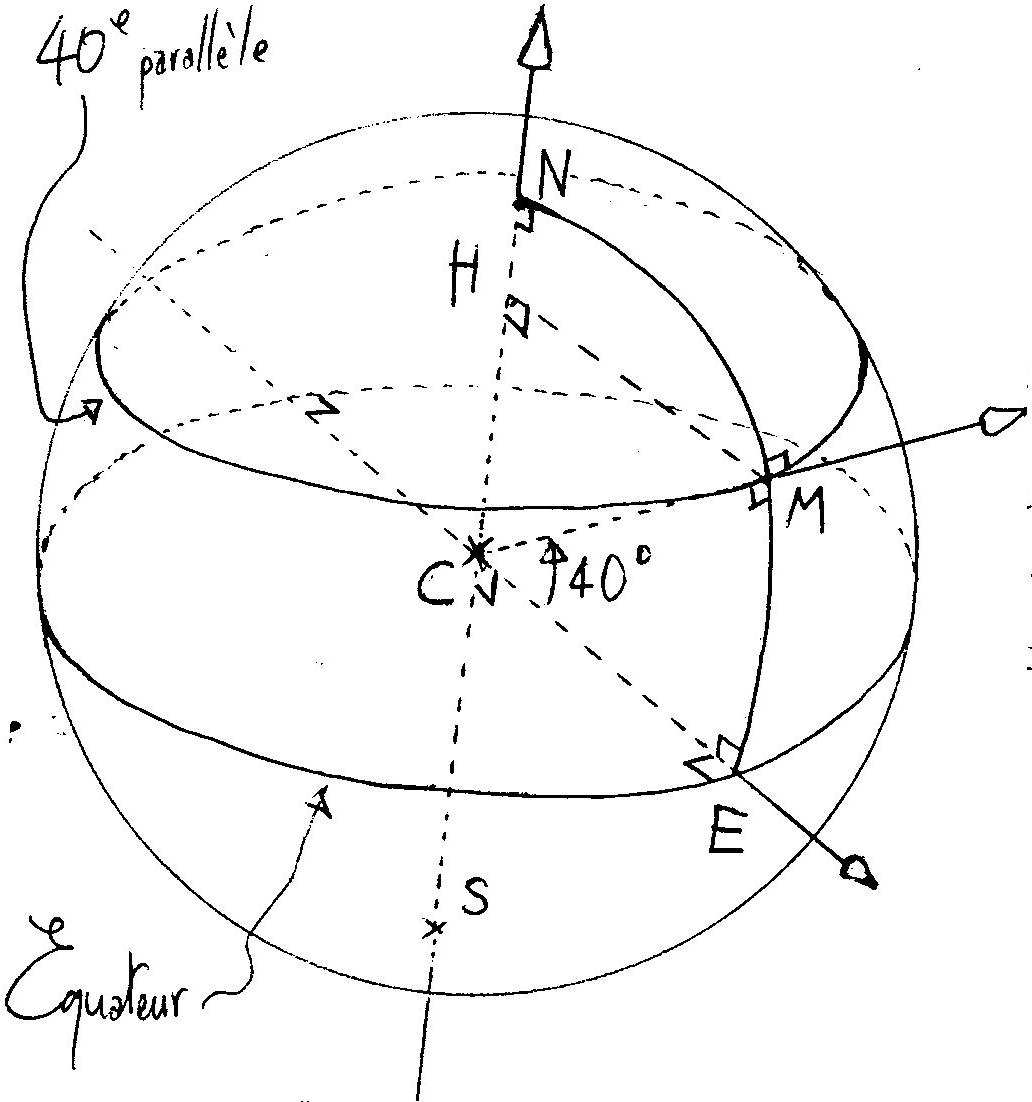
\includegraphics[width=0.6\textwidth]{image/fct_trigo/exo_trigo_sphere.jpg}
			
			\begin{enumerate}[1)]
				\item En sachant que $[HM]$ est un rayon du 40$^\e$ parallèle, calculer la longueur de ce parallèle à 100km près.
				\item Calculer la longueur du $x^\e$ parallèle en fonction de $x$ et de $R$. 
			\end{enumerate}


	\subsection{Formulaire de trigonométrie}
		\paragraph{Exercice } (Formules de trigonométrie)

		On étudie des manipulations algébriques fort utiles pour calculer les fonctions trigonométriques de valeurs particulières, ainsi que pour les problèmes physiques. On commence par exprimer les fonctions trigonométriques de la somme de deux angles, mettons $\alpha+\beta$, en fonction de $\sin\alpha$, $\sin\beta$, $\cos\alpha$ et $\sin\beta$ seulement. Même si la relation sera vraie pour tous angles orientés $\alpha$ et $\beta$ appartenant à $\R$, on effectue une preuve pour des angles orientés positifs tels que $\alpha+\beta<\frac{\pi}{2}$. L'extension de cette démonstration dans les autres cas est laissée au lecteur. On considère donc la figure \ref{fig_sin_add}.

		\begin{figure}
			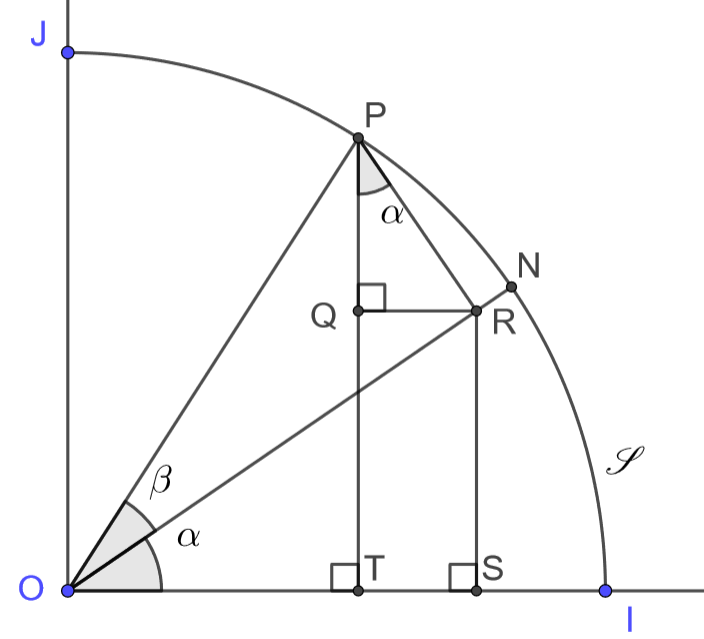
\includegraphics[width=0.5\textwidth]{image/fct_trigo/sin_addition.png} 
			\caption{Un cas particulier d'addition d'angles.}
			\label{fig_sin_add}
		\end{figure}
		

	\begin{enumerate}
		\item Calcul de $\sin(\alpha+\beta)$.
		\begin{enumerate}[a.]
			\item Vérifier rapidement que\,:
			\begin{equation}
			 	\sin(\alpha+\beta)=PQ+RS,\quad \sin\beta=PR,\quad \cos\beta=OR.
			\end{equation} 
			\item Démontrer que, comme indiqué sur la figure, $\widehat{QPR}=\alpha$, et en déduire que $\sin\alpha=\frac{RS}{OR}$.
			\item Exprimer $PQ$ et $PR$ en fonction de $\cos\alpha$, $\sin\alpha$, $\cos\beta$, $\sin\beta$.
			\item Conclure\,: exprimer $\sin(\alpha+\beta)$ en fonction de $\cos\alpha$, $\sin\alpha$, $\cos\beta$, $\sin\beta$.
		\end{enumerate}
		\item Extensions immédiates. Pour cette question, on utilisera abondamment les résultats de l'exercice 2 de la section \ref{subsec_sincos}.
		\begin{enumerate}[a.]
			\item En transformant $b$ en $-b$, calculer $\sin(\alpha-\beta)$ en fonction de $\cos\alpha$, $\sin\alpha$, $\cos\beta$, $\sin\beta$.
			\item En transformant $a$ en $\psd-a$, $b$ en $-b$, calculer $\cos(\alpha+\beta)$ en fonction de $\cos\alpha$, $\sin\alpha$, $\cos\beta$, $\sin\beta$.
			\item De même qu'en a., en déduire $\cos(\alpha-\beta)$.
		\end{enumerate}
		\item Formules de duplication, et de l'angle de moitié.
		\begin{enumerate}[a.]
			\item En considérant le cas où $\alpha=\beta$, calculer $\sin(2\alpha)$  en fonction de $\cos\alpha$ et $\sin\beta$.
			\item De même, calculer $\cos(2\alpha)$ en fonction de  $\cos\alpha$ et $\sin\beta$. En se souvenant que $\cos^2\alpha+\sin^2\alpha=1$, en déduire $\cos(2\alpha)$ en fonction de $\sin\alpha$ seulement, puis de $\cos\alpha$ seulement.
			\item Secouer les équations pour exprimer $\sin^2\alpha$ en fonction de $\cos(2\alpha)$, puis $\cos^2\alpha$ en fonction de $\cos(2\alpha)$
		\end{enumerate}
	\end{enumerate}

	\emph{Solutions} On donne les solutions sous la forme d'un formulaire de trigonométrie (circulaire). Certaines formules ne font pas partie de l'exercice, mais nous invitons tout de même le lecteur à les démontrer. $a$, $b$, $p$, $q$, sont des nombres réels, sauf dans les cas où ils compromettraient la définition d'une tangente ou d'un nombre avec dénominateur, auquel cas on laisse le lecteur adapter les définitions.

	\emph{Formules quadratiques}
	\begin{equation}
		\cos^2a+\sin^2a=1,\quad 1+\tan^2a=\frac{1}{\cos^2a}.
	\end{equation}
	\emph{Formules d'addition}
	\begin{equation}
		\cos(a+b)=\cos a\cos b -\sin a\sin b,\quad \sin(a+b)=\sin a \cos b + \sin b \cos a,
	\end{equation}
	\begin{equation}
		\cos(a-b)=\cos a \cos b + \sin a \sin b,\quad \sin(a-b)=\sin a \cos b - \sin b \cos a.
	\end{equation}
	\begin{equation}
		\tan(a+b)=\frac{\tan a+\tan b}{1-\tan a\tan b},\quad \tan(a-b)=\frac{\tan a-\tan b}{1+\tan a\tan b}
	\end{equation}
	\emph{Formules de duplication et de linéarisation}
	\begin{equation}
		\cos 2a = \cos^2a-\sin^2a=2\cos^2a-1=1-2\sin^2a,\quad 	\sin 2a=2\sin a \cos a,
	\end{equation}
	\begin{equation}
		\cos^2a=\frac{1}{2}+\frac{\cos a}{2},\quad \sin^2a=\frac{1}{2}-\frac{\cos 2a}{2}
	\end{equation}
	\begin{equation}
		\tan 2a=\frac{2\tan a}{1-\tan^2a}
	\end{equation}
	\emph{Formules du produit}
	\begin{equation}
		\cos a\cos b=\frac{1}{2}(\cos(a-b)+\cos(a+b)),\quad \cos a \sin b=\frac{1}{2}(\sin(a+b)-\sin(a-b)),
	\end{equation}
	\begin{equation}
		\sin a\sin b=\frac{1}{2}(\cos(a-b)-\cos(a+b)),
	\end{equation}
	\begin{equation}
		\cos p+\cos q=2\cos\frac{p+q}{2}\cos\frac{p-q}{2},\quad \cos p-\cos q=-2\sin\frac{p+q}{2}\sin\frac{p-q}{2},
	\end{equation}
	\begin{equation}
		\sin p +\sin q=2\sin\frac{p+q}{2}\cos\frac{p-q}{2},\quad \sin p -\sin q=2\sin\frac{p-q}{2}\cos\frac{p+q}{2}.
	\end{equation}
	\emph{Formules de la tangente de l'angle de moitié}
	On pose $t=\tan\frac{a}{2}$. Alors\,:
	\begin{equation}
		\cos a=\frac{1-t^2}{1+t^2}\quad \sin a=\frac{2t}{1+t^2},\quad \tan a=\frac{2t}{1-t^2}.
	\end{equation}
\paragraph{Application\,: valeurs numériques des fonctions trigonométriques.}
En utilisant ces formules de trigonométrie, on peut fabriquer des tables qui contiennent les valeurs des fonctions trigonométriques, uniquement à partir des valeurs remarquables calculées plus haut. Nous savons par exemple que $\cos\frac{\pi}{4}=\frac{\sqrt{2}}{2}$. De là, à partir de la formule de duplication, on calcule directement que
\begin{equation}
    \cos\frac{\pi}{8}=\sqrt{\frac{\cos\frac{\pi}{4}+1}{2}}=\sqrt{\frac{\frac{\sqrt{2}}{2}+1}{2}}.\nonumber
\end{equation}
Puis,
\begin{equation}
    \cos{\frac{\pi}{16}}=\sqrt{\frac{\cos\frac{\pi}{8}+1}{2}}=\sqrt{\frac{\sqrt{\frac{\frac{\sqrt{2}}{2}+1}{2}}+1}{2}}.\nonumber
\end{equation}
Bref, on peut montrer facilement que
\begin{equation*}
    \forall n\in\N, \cos\frac{\pi}{4\cdot 2^{n+1}}=\sqrt{\frac{\cos\frac{\pi}{4\cdot 2^n}+1}{2}}.
\end{equation*}
Et de même,
\begin{equation*}
    \forall n\in\N, \sin\frac{\pi}{4\cdot 2^{n+1}}=\sqrt{1-\frac{\cos\frac{\pi}{4\cdot 2^n}}{2}}.
\end{equation*}
Cela nous permet en principe de calculer les valeurs du cosinus de nombres aussi petits que l'on veut. Ensuite, si l'on cherche la valeur du cosinus d'un nombre $x\in\[0,\psd\]$, on peut approcher la valeur de $x$ à $\varepsilon$ près en choisissant un nombre $n$ tel que $\frac{\pi}{4\cdot 2^n}<\varepsilon$, et un nombre $k$ tel que $k\frac{\pi}{4\cdot 2^n}<x<(k+1)\frac{\pi}{4\cdot 2^n}$. En utilisant $k-1$ fois la formule d'addition pour le cosinus, à partir des valeurs de $\cos\frac{\pi}{4\cdot 2^n}$ et $\sin\frac{\pi}{4\cdot 2^n}$, on peut trouver les valeurs de $\cos \(k\frac{\pi}{4\cdot 2^n}\)\approx\cos x$ et de $\sin\(k\frac{\pi}{4\cdot 2^n}\)\approx \sin x$. En effet,
\begin{equation*}
    \cos\(k\frac{\pi}{4\cdot 2^n}\)=\cos\(\frac{\pi}{4\cdot 2^n}+\ldots+\frac{\pi}{4\cdot 2^n}\)
\end{equation*}
où il y a $k-1$ additions, et de même pour $\sin\(k\frac{\pi}{4\cdot 2^n}\)$.

On peut donc approcher toute valeur des fonctions trigonométriques avec des expressions qui ne font intervenir que des racines carrées. 

\paragraph{Approcher la valeur du nombre \pi}

C'est pour cette raison que la formule parachutée à la fin du chapitre \ref{chap_pinombre} (équation \eqref{eq_serpent}) n'était pas si \guil{circulaire} que cela. En effet, nous avions montré que 
\begin{equation*}
    \pi=\lim\limits_{n\to\infty}n\sin\(\frac{\pi}{n}\).
\end{equation*}
Mais en remplaçant $n$ par $4\cdot 2^n$, cette égalité devient

\begin{equation*}
    \pi=\lim\limits_{n\to\infty}4\cdot 2^n\sin\(\frac{\pi}{4\cdot 2^n}\).
\end{equation*}
Et nous avons alors un processus qui permet d'approcher la valeur du nombre $\pi$. En fait, si l'on déroule les calculs (exercice\,: le faire\,!), on trouvera des formules très similaires à celles du chapitre \ref{chap_pinombre}.


\section{Fonctions trigonométriques réciproques.}

	\subsection{Résolution d'équations trigonométriques}
		\begin{thm}
			Soient $u,v\in\R$. Alors\,:
			\begin{equation}
				\sin u=\sin v\Leftrightarrow ((u\equiv v[2\pi])\lor(u\equiv\pi-v[2\pi])),
			\end{equation}
			\begin{equation}
				\cos u=\cos w\Leftrightarrow ((u\equiv w[2\pi])\lor(u\equiv-w[2\pi])).
			\end{equation}
		\end{thm}
		\emph{Idée de preuve.} Pour démontrer ce théorème, il faudrait d'abord parler de continuité et de construction rigoureuse de nombres réels. Cela sera fait dans une prochaine session. On peut cependant donner une idée intuitive de la preuve en s'aidant des schémas suivants. Considérons un angle $u$ repéré sur le cercle trigonométrique et demandons-nous quels autres angles peuvent donner des sinus et des cosinus égaux. Sur la figure \ref{fig_egal_angles_trigo}, on voit que\footnote{Tout mathématicien rigoureux doit se méfier d'arguments tels que \guil{on voit que}\,!} l'angle $v=\pi-u$ égalise les sinus, tandis que l'angle $w=-u$ égalise les cosinus. Et bien sûr, il faut se rappeler que cela se fait à des tours complets près, d'où le modulo $2\pi$.

		\begin{figure}
			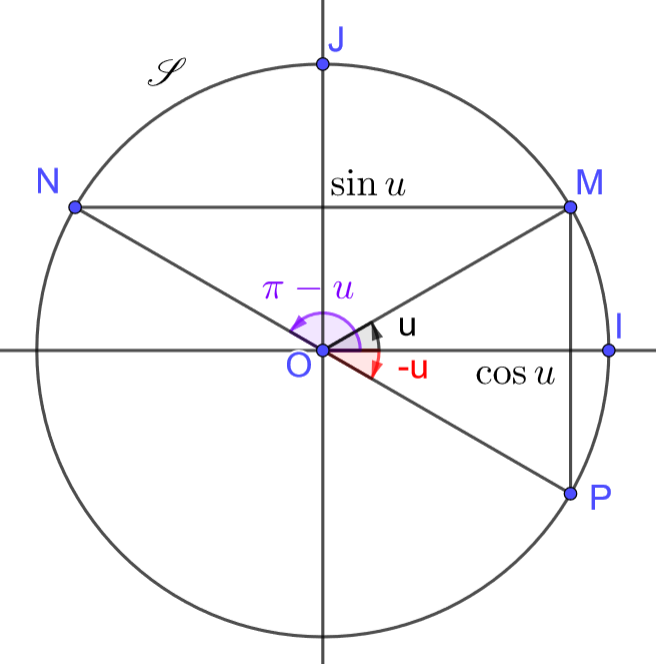
\includegraphics[width=0.5\textwidth]{image/fct_trigo/resol_eq_trigo.png}
			\caption{Résolution graphique d'équation trigonométrique. Ici, on a pris le cas où $0<u<\psd$. Nous invitons le lecteur à tracer les schémas des autres cas.}
			\label{fig_egal_angles_trigo}
		\end{figure}

		\paragraph{Exercice.} En s'aidant d'un tracer du cercle trigonométrique, résoudre les équations suivantes\,:
		\begin{equation}
			\cos x=\frac{\sqrt{3}}{2},\quad \sin x=-\frac{1}{2},\quad \cos 2x=\frac{\sqrt{2}}{2}.
		\end{equation}

		\emph{Solutions\,:}
		\begin{equation}
			\cos x=\frac{\sqrt{3}}{2}\Leftrightarrow x\equiv\pm\frac{\pi}{6}[2\pi],\quad\sin x=-\frac{1}{2}\Leftrightarrow\(x\equiv-\frac{\pi}{6}[2\pi]\lor x\equiv -\frac{5\pi}{6}[2\pi]\),
		\end{equation}
		\begin{equation}
			\cos 2x=\frac{\sqrt{2}}{2}\Leftrightarrow x\equiv\pm\frac{\pi}{8}[\pi].
		\end{equation}


	\subsection{Fonctions trigonométriques réciproques}
		\begin{thm}
			Soit $y\in[-1,1]$. Alors il existe un unique nombre réel $u$ dans l'intervalle $[0,\pi]$ tel que $y=\cos u$, et il existe un unique nombre réel $v$ dans l'intervalle $[-\pi,\pi]$ tel que $y=\cos v$. Par définition, on pose\,:
			\begin{equation}
				u=\acos y, \quad v=\asin y;
			\end{equation}
			$\acos$ est la fonction \emph{arc cosinus}, et $\asin$ est la fonction \emph{arc sinus}.

			Soit $z\in\R$. Alors il existe un unique nombre réel $w$ dans l'intervalle $\left]-\frac{\pi}{2},\frac{\pi}{2}\right[$, tel que $z=\tan w$. Par définition, on pose\,:
			\begin{equation}
				w=\atan z;
			\end{equation}
			$\atan$ est la fonction \emph{arc tangente}.
		\end{thm}

		La démonstration rigoureuse de ce théorème demande d'utiliser la notion de continuité des fonctions, qui sera vue dans la prochaine session de cours. Même si je dois vous demander de l'admettre, on peut quand même se convaincre \guil{visuellement} du résultat. En effet, en visualisant le cercle trigonométrique, si l'on contraint l'angle $u$ orienté à balayer l'intervalle $\[-\psd,\psd\]$, tout nombre $y$ compris entre $-1$ et $1$ sera atteint par $\sin u$ une et une unique fois, et si l'angle $v$ balaye l'intervalle $[0,2\pi]$, alors ce nombre $y$ sera atteint une et une unique fois par $\cos v$. Lorsque $w$ balaye l'intervalle $\left]-\psd,\psd\right[$, $\tan w$ balaye l'ensemble des nombres réels. On peut s'en convaincre en constatant que plus $w$ se rapproche de $-\psd$ sans jamais l'atteindre, plus $\tan w$ prend de grandes valeurs négatives, jusqu'à tendre vers $-\infty$\,; de même, lorsque $w$ se rapproche de $\psd$, $\tan w$ tend vers $+\infty$. Comme le nombre $\tan w$ ne fait que croître avec $w$, on peut comprendre intuitivement que tout nombre réel est atteint une et une unique fois par $\tan w$ lorsque $w$ balaye l'intervalle $\left]-\psd,\psd\right[$.

	\subsection{Représentation graphique des fonctions trigonométriques}
		Les fonctions $\sin$ et $\cos$ sont définies sur $\R$, il est possible de tracer leur graphe. On a déjà un début de tableau de valeurs, mais en plus, on sait qu'à chaque fois que l'argument de ces fonctions avance de $2\pi$, la fonction devient identique à elle-même. Autrement dit, $\forall x\in\R, \cos(x+2\pi)=\cos x, \sin(x+2\pi)=\sin x$. On n'a donc besoin de tracer ces fonctions que sur un intervalle de longueur $2\pi$, puis il suffit de reproduire le graphe à l'identique. Dans la figure \ref{fig_graphefcttrig}, on a représenté les graphes des fonctions $\cos$ et $\sin$.

		\begin{figure}
			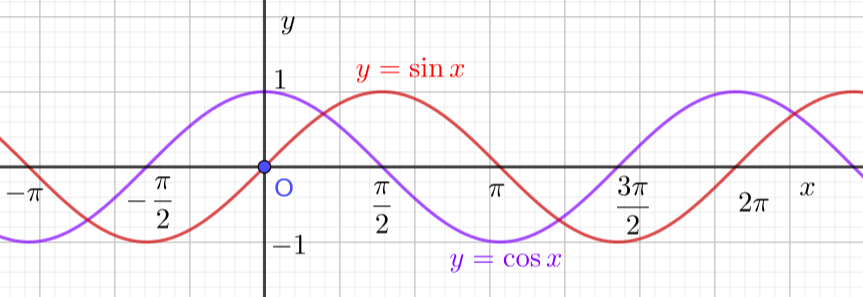
\includegraphics[width=0.8\textwidth]{image/fct_trigo/courbes_trigo.png}
			\caption{Représentation graphique des fonctions trigonométriques.}
			\label{fig_graphefcttrig}
		\end{figure}

		La fonction tangente a quelqu'originalité en plus, puisqu'elle diverge à chaque fois que l'on atteint $\pm\psd[\pi]$. Elle est définie sur $\R-\left\{\psd+k\pi,k\in\Z\right\}$, ou de manière plus synthétique, $\R-\left\{\psd+\pi\Z\right\}$. Sa courbe est représentée figure \ref{fig_plot_tan}.

		\begin{figure}
			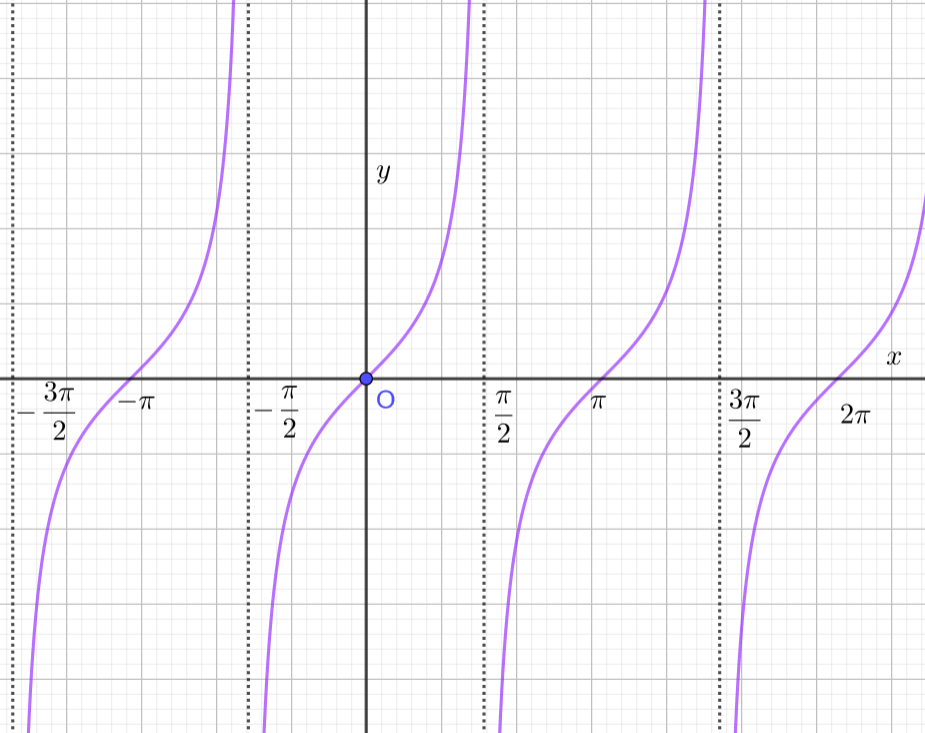
\includegraphics[width=0.8\textwidth]{image/fct_trigo/plot_tan.png}
			\caption{Représentation graphique de la fonction tangente. On a représenté en pointillé les lignes qui correspondent aux valeurs interdites, c'est-à-dire $\psd[\pi]$. On peut visualiser aisément les comportement \guil{infinis} au voisinage de ces points.}
			\label{fig_plot_tan}
		\end{figure}

		Le théorème suivant permet de tracer les fonctions réciproques. Nous en donnons l'illustration figures $\ref{fig_asincos}-\ref{fig_atan}$.

		\begin{thm}
			\begin{itemize}[label=\textbullet]
				\item Le graphe de la fonction $\asin$ est le symétrique du graphe de la fonction $\sin$ restreinte à l'intervalle $\[-\psd,\psd\]$, par rapport à la droite d'équation $y=x$.
				\item Le graphe de la fonction $\acos$ est le symétrique du graphe de la fonction $\cos$ restreinte à l'intervalle $[0,2\pi]$. 
				\item Le graphe de la fonction $\atan$ est le symétrique du graphe de la fonction $\tan$ restreinte à l'intervalle $\left]-\psd,\psd\right[$.
			\end{itemize}
			  
		\end{thm}
		\begin{proof}
			On ne démontre que le premier point, les autres s'effectuent de manière similaire. Considérons $\Gamma$ le graphe de la fonction $\sin$ restreinte à l'intervalle $\[-\psd,\psd\]$.  Pour tout $x\in\[-\psd,\psd\]$, le point de coordonnées $(x,\sin x)$ est sur ce graphe. Ceci étant donné, pour construire le graphe de la fonction $\asin$, il suffit d'inverser l'ordre des coordonnées, puisque cette fonction a pour objet de transformer $y=\sin x$ en $x=\acos y$. En effet, soit $y\in [0,1]$. Il existe un unique $x\in\[-\psd,\psd\]$ tel que $\sin x=y$, et on a $y=\asin x$. Donc le point de coordonnée $(x,y)$ appartient à $\Gamma$, et le point de la courbe souhaitée s'obtient par inversion de l'ordre des coordonnées, et donc, par symétrie d'axe $(d)$ où $(d)$ a pour équation $y=x$. 

			Les autres graphes se construisent de manière similaire. En fait, toute fonction réciproque se trace par symétrie autour de $(d)$. 
		\end{proof}


		\begin{figure}
			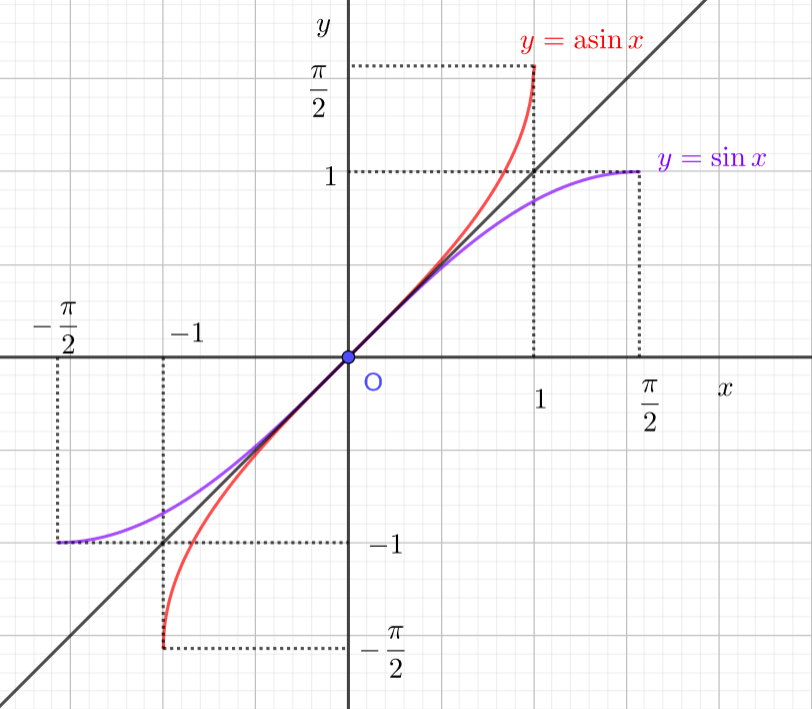
\includegraphics[width=0.55\textwidth]{image/fct_trigo/courbe_asin.png} 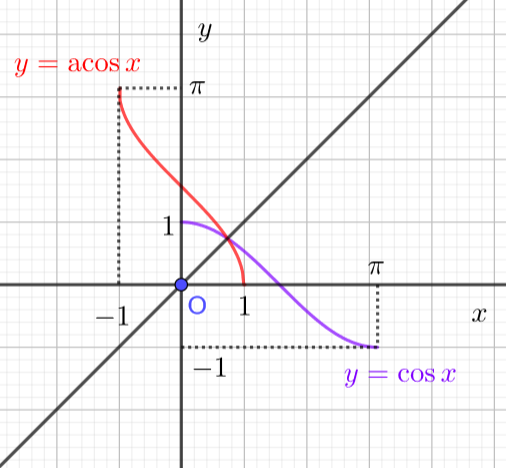
\includegraphics[width=0.43\textwidth]{image/fct_trigo/courbe_acos.png}
			\caption{À gauche\,: graphe de la fonction $\asin$ construit à partir de celui de $\sin$. À droite\,: idem pour $\acos$ et $\cos$.}
			\label{fig_asincos}
		\end{figure}
		\begin{figure}
			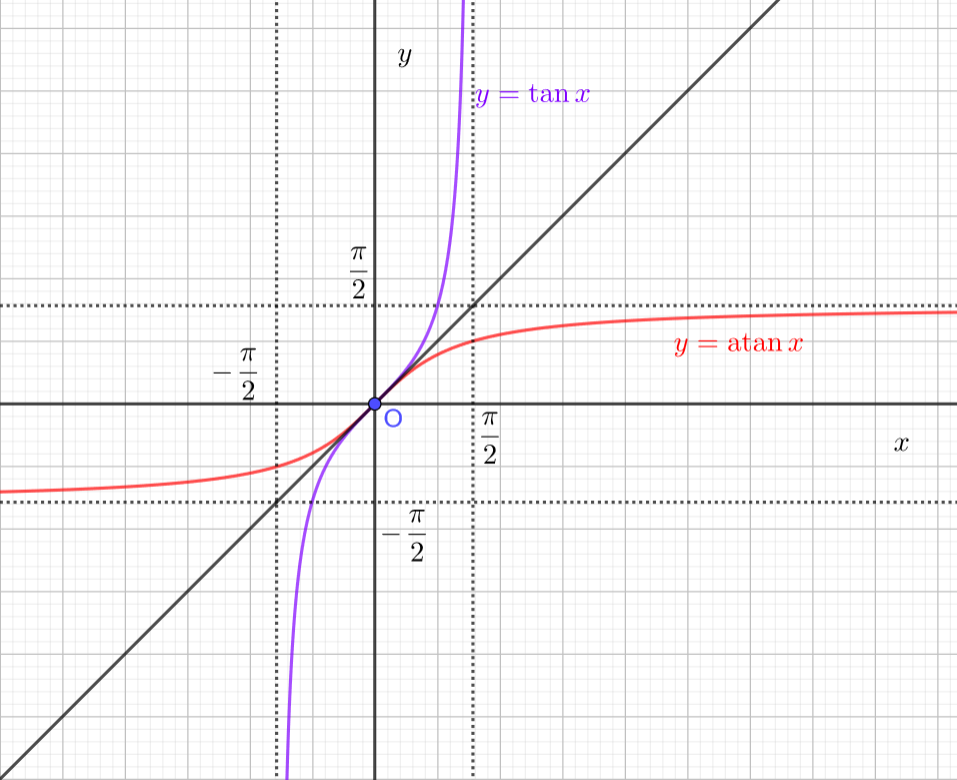
\includegraphics[width=0.8\textwidth]{image/fct_trigo/courbe_atan.png}
			\caption{Représentation graphique de la fonction $\atan$ à partir de celui de $\tan$.}
			\label{fig_atan}
		\end{figure}

		\vspace{0.3cm}

		Les fonctions trigonométriques réciproques permettent de calculer des angles, lorsque l'on connaît uniquement leurs cosinus et sinus. C'est ainsi que lorsque vous étiez petits, on vous demandait de calculer les angles d'un triangle rectangle dont les mesures des côtés étaient données. Considérons un triangle $ABC$ rectangle en $B$, mettons que l'on connaisse deux grandeurs, par exemple $AB=a$, $AC=b$ (on pourrait déduire la troisième via le théorème de Pythagore, mais peu importe). Alors, puisque $\cos\widehat{BAC}=\frac{AB}{AC}=\frac{a}{b}$, on a directement $\widehat{BAC}=\acos\(\frac{a}{b}\)$. Si l'on ne connaissait que $AB=a$ et $BC=c$, alors puisque $\tan\widehat{BAC}=\frac{BC}{AB}=\frac{c}{a}$, on déduit également que $\widehat{BAC}=\atan\(\frac{c}{a}\)$. Et enfin, de même, on montre que $\widehat{BAC}=\asin\(\frac{c}{b}\)$. C'est la principale utilité des fonctions trigonométriques réciproques. Mais on peut également s'amuser à démontrer des relations algébriques\,:

		\paragraph{Exercice.} Démontrer que\,:
		\begin{enumerate}
			\item $\forall x\in\[0,1\], \acos x+\asin x=\psd$,
			\item $\forall x\in[-1,1], \cos(\asin x)=\sin(\acos x)=\sqrt{1-x^2}$,
			\item 
			\begin{equation}
				\forall x\in]-1,1[,\quad  \tan(\asin x)=\frac{x}{1-x^2},\quad\forall x\in]-1,1[-\{0\},\quad  \tan(\acos x) = \frac{\sqrt{1-x^2}}{x},
			\end{equation}
			\item 
			\begin{equation}
				\forall x\in\R,\quad \sin(\atan x)=\frac{x}{\sqrt{1+x^2}},\quad \cos(\atan x)=\frac{1}{\sqrt{1+x^2}}.
			\end{equation}
		\end{enumerate}
		 

		\noindent\emph{Solution.} 
		\begin{enumerate}
			\item Soit $x\in[0,1]$. $\exists ! \theta\in\[0,\psd\],x=\cos \theta$, et de plus, $\acos x = \theta$. Mais comme $\cos \theta=\sin\(\psd-\theta\)=x$, on a $\asin x=\psd-\theta=\psd-\acos x$. D'où le résultat.
			\item $\acos$ est une fonction positive comprise entre $0$ et $\pi$, donc $\forall x\in[-1,1], \sin(\acos x)\ge 0$. De là, il suffit d'écrire que $\cos^2(\acos x)+\sin^2(\acos x)=1=x^2+\sin^2(\acos x)$, d'où la deuxième égalité. La première se démontre de manière similaire.
			\item Il suffit d'écrire que $\tan(\asin x)=\frac{\sin(\asin x)}{\cos(\asin x)}$ et d'utiliser la question précédente. On procède de même pour la deuxième égalité.
			\item Considérons un triangle rectangle $ABC$ rectangle en $B$, notons $\alpha$ l'angle au sommet de $A$. Supposons que $AB=1$ et $BC=x>0$ (le cas $x<0$ se traite aisément en utilisant les propriétés des fonctions trigonométriques). Alors $AC=\sqrt{1+x^2}$, $\sin\alpha=\frac{x}{\sqrt{1+x^2}}$, mais $\tan\alpha=x/1=x$, donc $\alpha=\atan x$, d'où le résultat. On procède de même pour la deuxième égalité.
		\end{enumerate}
		
		

\section{Utilité de la trigonométrie en Mécanique}
La Mécanique est l'art d'étudier le mouvement des corps matériels. C'est une branche de la science physique, dont l'objet est d'étudier les rapports quantitatifs entre des grandeurs mesurables des corps matériels afin d'en extraire des lois universelles et univoques.

	\subsection{Mouvement de rotation uniforme et roulement sans glissement}
		On considère une roue de rayon $R$ qui a un mouvement de rotation constant, et qui effectue un tour complet pendant la durée $T$. Le centre et l'axe de la roue sont fixés. On nomme $O$ ce centre, et on considère un repère orthonormé $(O,I,J)$ fixe par rapport à un observateur (il ne suit pas le mouvement de rotation) dans le même plan que la roue. On note $t$ la date qu'affiche un chronomètre lancé à $t=0$. Par convention, si un point $M$ a un mouvement qui dépend de la variable temporelle $t$, on exprimera cette dépendance en utilisant les notations des fonctions, et on notera $M(t)$ la position du point $M$ à la date $t$.
		\begin{enumerate}
			\item Montrer qu'un point $M(t)$ à l'extrémité de la roue tel que $M(0)$ a pour coordonnées $(R,0)$, a pour coordonnées à la date $t$\,: $(R\cos\omega t, R\sin\omega t)$, où on exprimera $\omega$ en fonction de $t$.
			\item En calculant la distance que fait le point $M$ pendant la durée $T$, calculer sa vitesse.
			\item Désormais on suppose que la roue roule sur le sol sans glisser. Cela signifie que le mouvement d'ensemble de la roue est tel que sa vitesse $v$ compense exactement la vitesse à l'extrémité de la roue, de telle sorte que la différence de vitesse entre l'extrémité de la roue qui touche le sol, et le sol, est nulle.
			\begin{enumerate}[a.]
			 	\item En déduire une relation entre $v$ et $\omega$.
			 	\item Calculer les coordonnées du point $O$ en fonction de $t$, sachant que $O(0)=(0,R)$ (on suppose que le sol est représenté par l'axe des abscisses).
			 	\item Par conséquent, le point $M(t)$ est tel que $M(0)$ a pour coordonnées $(R,R)$. En ajoutant le mouvement d'ensemble selon l'axe des abscisses $(Ox)$, démontrer que les coordonnées de $M(t)$ sont $(R(\cos(\omega t)-\omega t), R\sin \omega t)$.
			\end{enumerate} 
		\end{enumerate}
		La trajectoire d'un tel point est communément appelée \guil{cycloïde}. On représente cela figure \ref{fig_cyclo}.

		\begin{figure}
			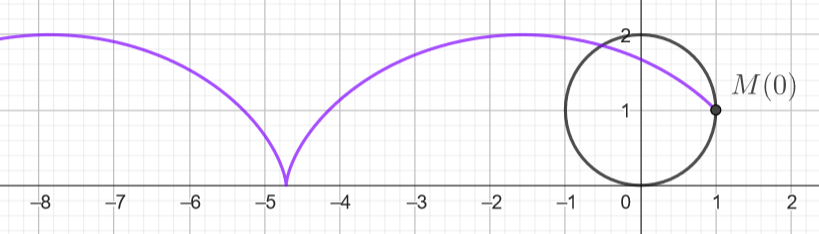
\includegraphics[width=0.6\textwidth]{image/fct_trigo/cyclo1.png}\\
			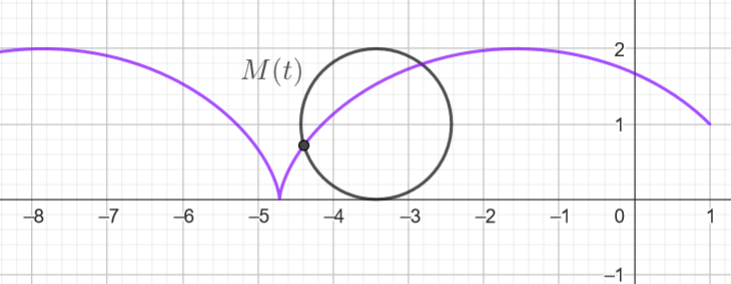
\includegraphics[width=0.6\textwidth]{image/fct_trigo/cyclo2.png}\\
			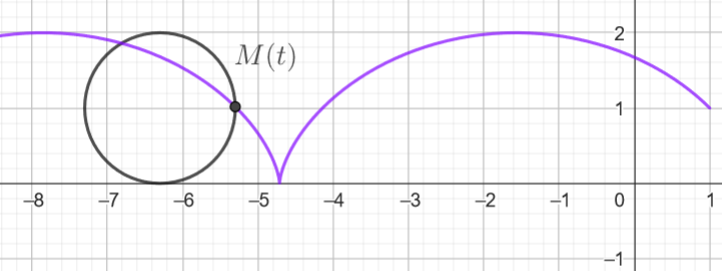
\includegraphics[width=0.6\textwidth]{image/fct_trigo/cyclo3.png}
			\caption{Représentation de la cycloïde et du cercle à trois instants. En haut\,: à $t=0$. En bas\,: à $t=\frac{2\pi}{\omega}$, la roue a réalisé un tour complet. Au milieu\,: date intermédiaire. On remarque que, puisque la roue tourne dans le sens trigonométrique, elle roule vers la gauche. On peut trouver moult animations de la cycloïde sur internet.}
			\label{fig_cyclo}
		\end{figure}

\iffalse
	\subsection{Loi de réfraction de Descartes}
		Tout le monde a fait l'expérience de l'illusion du bâton cassé lorsqu'il est plongé dans l'eau. Cela vient du fait que dans les milieux transparents, la lumière se propage plus lentement que dans le vide. Dans le vide, la célérité\footnote{En physique ondulatoire on préfère parler de célérité que de vitesse lorsqu'il s'agit de propagation d'une onde.} de la lumière vaut exactement $c=299\,792\,458$m/s. Dans un milieu $A$, la célérité de la lumière mesure $c_A<c$, et on défini l'indice de réfraction du milieu $A$ comme étant égal au rapport entre $c$ et $c_A$\,: $n_A=\frac{c}{c_A}$. Ainsi, l'indice de réfraction du vide vaut $1$ et tous les milieux transparents ont un indice de réfraction plus grand que $1$. Cette différence de vitesse de propagation implique des déviations de rayons lumineux. En physique ondulatoire, on peut démontrer que les trajectoires des rayons lumineux suivent ce que Fermat avait pris pour postulat\,:
		\begin{post}[Principe de Fermat]
			Lorsqu'un rayon lumineux peut relier deux points $A$ et $B$, il le fait en prenant le chemin optique qui minimise localement\footnote{Vu qu'il s'agit d'une minimisation locale, la lumière peut donc prendre plusieurs chemins. On verra quelques exemples plus bas.} la durée du parcours de la lumière\footnote{En vérité, une maximisation conviendrait aussi, mais dans presque tous les cas pratiques, il s'agit d'une minimisation.}
		\end{post}

		À présent considérons un miroir plan, un point $A$ et un point $B$. Bien sûr, la ligne droite qui relie $A$ et $B$ convient pour un rayon lumineux. Mais on sait que la lumière peut se réfléchis sur le miroir. Soit $M$ le point du miroir en lequel le rayon se réfléchit. On peut tracer $B'$, le symétrique de $B$ par rapport au plan du miroir. On a $AM+MB=AM+MB'$. Soit $M_0$ le point du miroir tel que $A$, $M_0$ et $B'$ soient alignés. Si le point $M$ est différent du point $M_0$, par inégalité triangulaire, le chemin réalisé sera plus long. Donc $M_0$ est le point solution. Par construction, on vérifie donc la loi suivante\,:
		\begin{thm}
			Lorsque la lumière se réfléchit sur un miroir plan, elle le fait en conservant l'angle d'attaque.
		\end{thm}

		Maintenant considérons une étendue d'air et une étendue d'eau séparées par un plan. L'air étant très peu dense, on pourra considérer que son indice de réfraction mesure 1. Ce n'est pas le cas de l'eau, donc nous considérerons son indice $n_e$. Soient $A$ et $B$ deux points, l'un étant dans l'air et l'autre dans l'eau, de telle sorte que $(AB)$ ne soit pas perpendiculaire à la surface de séparation (autrement il n'y aurait rien à faire). La question est\,: quel point $M$ minimise la durée du parcours\,? 
		\begin{enumerate}
			\item Calculer la durée du parcours que met la lumière à parcourir le segment $[AM]$ puis $[MB]$ en fonction de $n_e$, sachant que dans l'eau, la célérité de la lumière vaut $c_e$ et que $n_e=c/c_e$.
			\item 
		\end{enumerate}
\fi


	\subsection{Calcul d'une distance par parallaxe.}
		Les étoiles sont si loin de la Terre qu'il a été difficile de mesurer leur distance jusqu'au XIXe siècle. Il est possible de mesurer la distance de certaines étoiles par la méthode de la parallaxe. 
		Pour cela, on utilise la géométrie de l'orbite de la Terre, que l'on assimile à un cercle. 
		Pour simplifier les calculs, on a pris une étoile particulière, située en , dont la position est telle que  est la médiatrice de  (voir figure \ref{fig_par}). Dans la figure, A et B représentent la position de la Terre à six mois d’écart, et S représente le Soleil. Attention, la figure n’est pas à l’échelle.




		\begin{figure}
			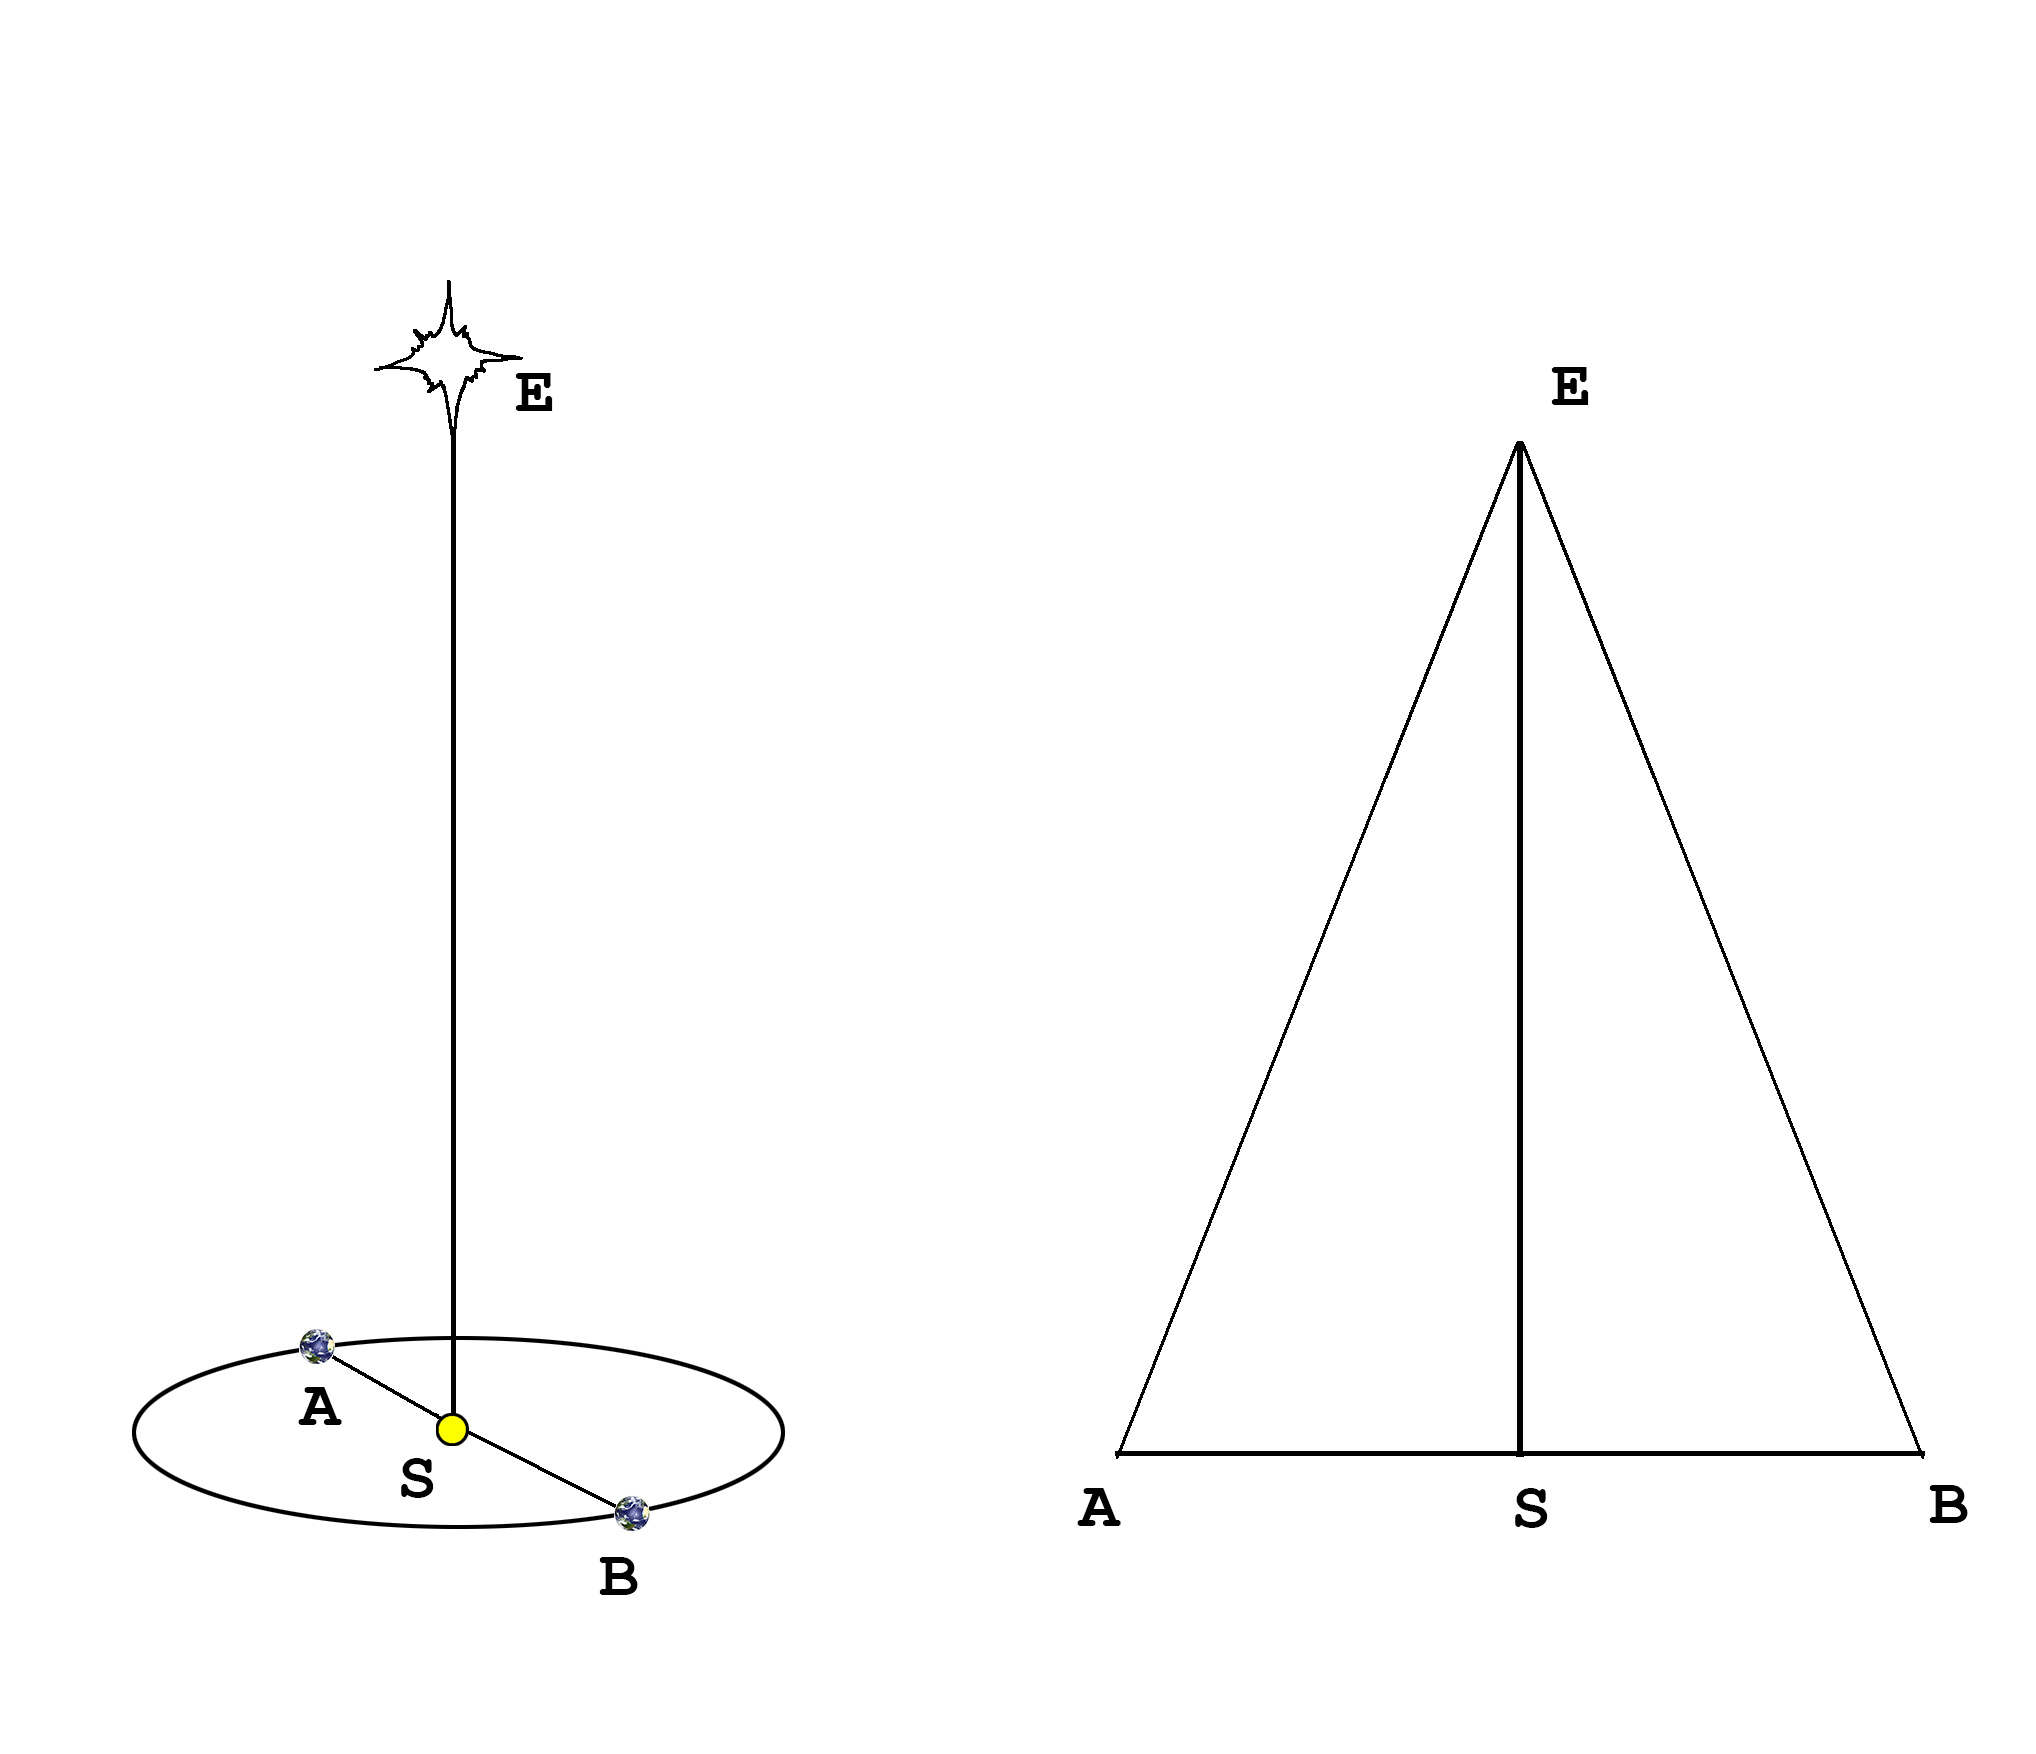
\includegraphics[width=0.6\textwidth]{image/fct_trigo/fig2_parallaxe.jpg}
			\caption{Représentation (pas à l'échelle) d'un cas parcitulier de parallaxe. À gauche\,: figure en perspective. À droite\,: figure plane.}
			\label{fig_par}
		\end{figure}


		Une minute d’arc d’angle mesure un soixantième de degré\,: $1'=\frac{1}{60}^\circ$. Une seconde de degré mesure un soixantième de minute de degré\,: $1''=\frac{1}{60}'$. Ainsi, $1''=\frac{1}{3600}^\circ$. 
		On mesure $\widehat{SEB}=0.02''$. On sait que le rayon de l’orbite terrestre mesure environ $150\cdot 10^6$km.

		\begin{enumerate}
			\item Calculer $EB$ en km.
			\item Si on avait voulu faire un schéma à l’échelle avec $EB=20$cm, combien aurait dû mesurer $AB$ sur le schéma\,? Aurait-on pu faire un schéma à l’échelle sur une feuille A4\,?
			\item Maintenant on s'intéresse à une mesure de parallaxe quelconque (voir figure \ref{fig_par_vrai}). Sachant que l'on mesure les angles $\alpha=\widehat{ST_1E}$, $\beta=\widehat{ST_2E}$, et que l'on connaît le rayon $R$ de l'orbite de la Terre, calculer $T_1E$ et $T_2E$ en fonction des grandeurs connues.
		\end{enumerate}

		\begin{figure}
			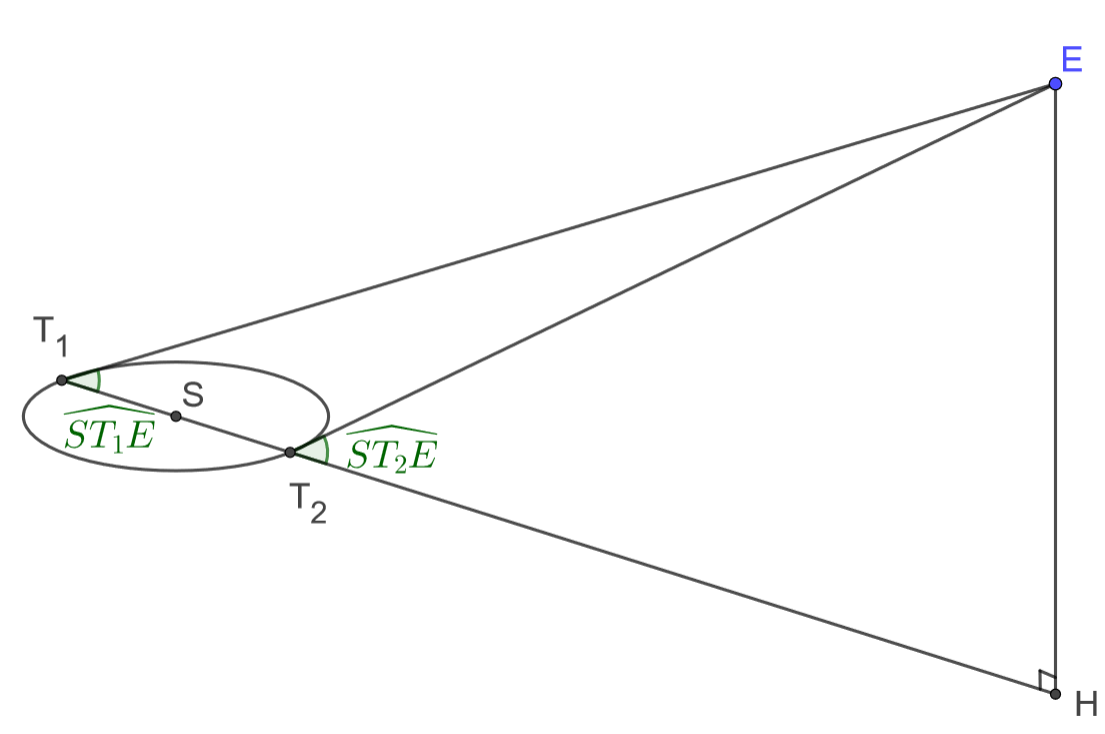
\includegraphics[width=0.6\textwidth]{image/fct_trigo/fig1_parallaxe.png}
			\caption{Situation générale de mesure par parallaxe, en perspective. Les points $T_1$, $S$, $T_2$, $E$, et $H$ sont dans le même plan.}
			\label{fig_par_vrai}
		\end{figure}






%%%%%%%%%%%%%%%%%%%%%%%%%%%%%%
%Bibliography
%%%%%%%%%%%%%%%%%%%%%%%%%%%%%
\addcontentsline{toc}{chapter}{Bibliographie}  %Tout ce bazar permet d'avoir l'intro dans la table des matières sans la numéroter
\markboth{Bibliographie}{Bibliographie}
%\printbibliography[heading=bibintoc]
\bibliographystyle{unsrt-fr}
\bibliography{biblio}


\part*{Annexes}
\appendix

\appendix

\chapter{Annexe de la partie 1. Rappels\,: ensembles de nombres.}\label{app_nbs}

	\section{Nombres entiers naturels}
		Les nombres naturels servent à compter des quantités dénombrables. Ils ont été l'objet de la première séance de \guil{maths-champignons}. Nous en donnons une définition concise ici, qui prend le risque d'être circulaire.
		\begin{defi}
			L'ensemble des nombres entiers naturels est l'ensemble des nombres que l'on peut obtenir, partant de zéro, par une succession arbitraire d'additions d'unité.

			Cet ensemble est noté symboliquement $\N$.
		\end{defi}
		\paragraph{Remarques.} 

		\begin{itemize}[label=\textbullet]
			\item Dans cette définition, on considère \guil{succession arbitraire} au sens large, en y incluant l'absence de succession. Ce qui fait que $O$ est également un entier naturel.
			\item Dans de nombreux livres de mathématiques, on peut souvent lire\,: $\N=\{0;1;2;\ldots\}$. En fait, presque tous les nombres entiers naturels sont dans les \guil{\ldots}\,!!! 
		\end{itemize}	


		Partant du repère cartésien à une dimension, on peut proposer cette définition alternative\,:
		\begin{defi}
			Considérons une droite graduée $(O;I)$ où par convention, $OI$ représente l'unité. L'ensemble des nombres entiers naturels est l'ensemble des abscisses des points obtenus par une succession quelconque de translations de bipoint $(O;I)$ --- c'est-à-dire la translation qui transforme $O$ en $I$.
		\end{defi}

		Nous donnons une illustration géométrique de cette définition ci-dessous.
		
		\includegraphics[width=0.5\textwidth]{image/calcul/ens_N.png} 

	\section{Nombres entiers relatifs}
		L'ensemble des nombres entiers relatifs introduit la notion de nombres négatifs. Pour les introduire, on peut considérer le problème suivant\,: trouver un nombre $a$ tel que $3+a=2$ (nous laissons le lecteur réfléchir à ce problème).

		\begin{defi}
			L'ensemble des nombres entiers relatifs est l'ensemble des nombres qui peuvent s'obtenir, partant de zéro, par successions arbitraires d'additions ou soustractions d'unité.

			De manière équivalente, étant donné une droite graduée $(O;I)$ avec $OI$ l'unité, c'est l'ensemble des abscisses des points qui peuvent être obtenus, partant de $O$, par une succession arbitraire de translations de bipoints $(0;I)$ ou $(I;O)$.

			Cet ensemble est noté $\Z$.
		\end{defi} 

		\paragraph{Remarque.} Dans les livres de mathématiques, on lit souvent \\ $\Z=\{\ldots;-3;-2;-1;0;1;2,3;\ldots\}$. Même remarque\,: presque tous les nombres sont cachés dans les \guil{\ldots}.

		\vspace{0.3cm}

		On donne une illustration de l'ensemble $\Z$ ci-dessous.

		\includegraphics[width=0.8\textwidth]{image/calcul/ens_Z.png}


	\section{Nombres rationnels}
		Considérons deux nombres entiers $p$ et $q$ avec $q$ non nul. Nous allons proposer une construction géométrique qui permet de placer un point dont l'abscisse est le résultat de la division de $p$ par $q$.

		Placer deux points $O$, $I$ distincts sur le plan. Tracer une droite numérique orientée $(O;I)$. $OI$ sera l'unité. Placer un autre point $J$ hors de la droite $(OI)$ tel que $OJ=OI$. Tracer la droite numérique orientée $(O;J)$. Il n'est pas nécessaire que $(OI)\perp (OJ)$. Sur la droite numérique $(O;I)$, placer le point $P$ d'abscisse $x_P=p$. Sur la droite numérique $(O;J)$, placer le point $Q$ d'abscisse $x_Q=q$. Tracer la droite $(JP)$. Tracer la droite $(d)$ passant par $Q$ et parallèle à la droite $(JP)$. Placer $A=(d)\cap(OI)$. Alors l'abscisse de $A$ vaut $p/q$ (illustration figure \ref{fig_psq}).

		\begin{figure}
			\includegraphics[width=0.6\textwidth]{image/calcul/constr_psq.png}
			\caption{Pour cette construction, on a pris $p=2$ et $q=3$. L'abscisse de $A$ vaut donc $2/3$.}
			\label{fig_psq}
		\end{figure}

		\begin{proof}
			On se contente de démontrer le résultat dans le cas où $p$ et $q$ sont strictement positifs. Nous laissons les autres cas aux lecteurs, les démonstrations étant analogues.

			Les cas $p=q=1$ étant triviaux, on suppose que $p$ ou $q$ est strictement supérieur à 1. Dans ce cas, les points $O$, $A$, $P$ sont alignés dans le même ordre que les points alignés $O$, $J$ $Q$ (sinon, les droites $(JA)$ et $(PQ)$ seraient sécantes). Comme les droites $(JA)$ et $(PQ)$ sont parallèles, on peut utiliser le théorème de Thalès\,:
			\begin{equation}
				\frac{OA}{OP}=\frac{OJ}{OQ}
			\end{equation}
			Donc
			\begin{equation}
				\frac{OA}{OJ}=\frac{OA}{OI}=\frac{OP}{OQ}=\frac{p}{q}
			\end{equation}
			(car $OI=OJ$). Et donc, l'abscisse du point $A$ est bien $p/q$.
		\end{proof}

		On peut en déduire la définition suivante\,:
		\begin{defi}
			L'ensemble des nombres rationnels est l'ensemble des abscisses des points qui peuvent s'obtenir par la construction précédente, avec $p\in\Z$, et $q\in\N\backslash\{0\}$ (tous les nombres entiers naturels sauf $0$).

			On note $\Q$ cet ensemble.

			De manière équivalente, on peut écrire\,:
			\begin{equation}
				\Q=\left\{\left.\frac{p}{q}\right|p\in\Z, q\in\N\backslash\{0\}\right\},
			\end{equation}
			soit l'ensemble des nombres qui peuvent s'écrire sous la forme d'un quotient de nombres entiers.

		\end{defi}

	\section{Nombres décimaux}
		Les nombres décimaux sont les nombres utilisés par les physiciens. De manière intuitive, ce sont les nombres qui peuvent s'écrire avec \guil{un nombre fini de chiffres après la virgule}. Cela signifie qu'on a une précision limitée. On peut écrire cela de manière plus formelle.

		\begin{defi}
			Soit $(O;I)$ une droite graduée avec $OI$ l'unité. L'ensemble des nombres décimaux est l'ensemble des abscisses des points qui peuvent correspondre à un ensemble arbitraire de subdivisions récursives des intervalles entres les nombres entiers relatifs. 

			On note $\D$ cet ensemble de nombres.

			Autrement dit, 
			\begin{equation}
				\D=\left\{\left.\frac{a}{10^n}\right| a\in\N, n\in\Z\right\}
			\end{equation}
		\end{defi}

		\paragraph{Remarque.} Certains nombres rationnels sont aussi des nombres décimaux. Par exemple, $1/5=0.2$. En revanche, certains nombres rationnels, si on voulait les écrire sous forme décimale, auraient un nombre infini de chiffres après la virgule. En effet, lorsqu'on pose et qu'on effectue la division de 1 par 3, on trouve que $1/3=0.333\ldots$ à l'infini.

		\begin{thm}
			Soit $r/q$ la fraction irréductible d'un nombre rationnel. Alors ce nombre est décimal si et seulement si $q$ peut s'écrire sous la forme $2^k5^\ell$ où $k$ et $\ell$ sont des nombres entiers naturels. En langage plus formel\,:
			\begin{equation}
				\frac{r}{q}\in\D \Leftrightarrow \exists k,\ell\in\N, q=2^k5^\ell.
			\end{equation}
		\end{thm}
		\begin{proof}
			On présente deux démonstrations. La première procède par double inclusion d'ensembles, la seconde utilise des théorèmes classiques d'arithmétique.
			
			\noindent\emph{Première démonstration\,: double inclusion.}

			Soit $\D_0$ l'ensemble des nombres qui peuvent s'écrire sous la forme $\frac{a}{2^k5^\ell}$, où $a\in\Z, k,\ell\in\N$. Nous allons montrer que $\D_0=\D$. Pour montrer que deux ensembles sont égaux, il faut montrer que l'un est inclus dans l'autre et que l'autre est inclus dans l'un. Formellement, il faut donc montrer que $\D_0=\D\Leftrightarrow (\D\subset\D_0\wedge\D_0\subset\D)$. Alors, on aura démontré que tout nombre dans $\D$ peut s'écrire comme le demande le théorème, et que tout  nombre écrit comme le demande le théorème est bien un nombre décimal.

			Démontrons que $\D_0\subset\D$. Soit un nombre $x$, arbitraire, appartenant à $\D_0$\,; nous allons démontrer qu'il appartient aussi à $\D$. Comme $x\in\D_0$, on peut écrire $x=\frac{a}{2^k5^\ell}$. Mais\,:
			\begin{equation}
				x=\frac{a}{2^k5^\ell}=\frac{a}{2^k5^\ell}\cdot\frac{2^{k\ell}5^{k\ell}}{2^{k\ell}5^{k\ell}}=\frac{a 2^{k\ell-k}5^{k\ell-\ell}}{2^{k\ell}5^{k\ell}}=\frac{a2^{k\ell-k}5^{k\ell-\ell}}{(2\times 5)^{k\ell}}=\frac{a2^{k\ell-k}5^{k\ell-\ell}}{10^{k\ell}},
			\end{equation}
			le numérateur étant un nombre entier et le dénominateur une puissance de dix, on a bien $x\in\D$. Donc $\D_0\subset\D$.

			Démontrons maintenant que $\D\subset\D_0$. Soit $y\in\D_0$\,; on peut écrire $y=\frac{b}{10^n}$ où $b\in\Z$ et $n\in\N$. Alors\,:
			\begin{equation}
				y=\frac{b}{10^n}=\frac{b}{(2\times 5)^n}=\frac{b}{2^n5^n}
			\end{equation}
			donc $b\in\D_0$. Donc $\D\subset\D_0$

			Conclusion\,: $\D=\D_0$.

			\noindent\emph{Deuxième démonstration\,: arithmétique.}
			
			$\Leftarrow$ On sait que $1/5=0.2$ et que $1/2=0.5$. $\D$ est stable par multiplication, donc pour tous $k,\ell\in\N$, $r/(2^k5^\ell)\in\D$.

			$\Rightarrow$ ($\star$) Pour démontrer l'implication directe, on va procéder par contraposition absurde\,: on va démontrer la contraposée (que si le dénominateur ne s'écrit pas comme un produit de 2 et de 5, alors la fraction n'est pas rationnelle) par l'absurde (on va supposer que le dénominateur du nombre ne s'écrit pas ainsi mais est quand même rationnel, et aboutir à une contradiction).

			Soit donc
			\begin{equation}
				q=\prod_i p_i^{k_i}
			\end{equation} 
			la décomposition en facteurs premiers du dénominateur de $r/q$. Supposons que les $p_i$ ne soient pas que des diviseurs de 10, soit $p$ l'un d'entre eux (non diviseur de 10). On récrit $q=p^kS$, avec 
			\begin{equation}
			 S=\prod_{p_i\ne p}p_i^{k_i}.\end{equation} 
			Supposons que $r$ soit un nombre décimal. Alors, on aurait
			\begin{equation}
				\frac{a}{10^n}=\frac{r}{p^kS}
			\end{equation}
			avec $a\in\Z$ et $n\in\N$, et donc $ap^kS=r10^n$ (axiome du produit en croix).
			La fraction étant réputée irréductible, $p$ et $r$ sont premiers entre eux, donc $p^k$ est un diviseur de $10^n$, or la décomposition (unique) en facteurs premiers de $10^n$ est $2^n5^n$, donc $p=2$ ou $p=5$. Mais on avait supposé que $p$ n'était pas un diviseur de 10. Contradiction. 
		\end{proof}

	\section{Nombres réels}
		Comme nous l'avons vu lors de \guil{maths-champignons}, il existe des nombres irrationnels, c'est-à-dire qu'on peut construire des longueurs qui ne peuvent pas s'exprimer sous la forme d'un rapport de nombres entiers. De manière synthétique (nous développerons ce point dans une session ultérieure de notre école de mathématiques), on peut dire que l'ensemble des nombres réels constitue \guil{toutes} les abscisses possibles sur la droite graduée.

	\section{Résultats sur les ensembles de nombres.}

		\begin{thm}
			$\N\subset\Z\subset\D\subset\Q\subset\R$. Cela signifie que l'ensemble $\N$ est contenu dans l'ensemble $\Z$, qui lui-même est contenu dans $\D$, lui-même contenu dans $\Q$, lui-même contenu dans $\R$.
		\end{thm}
		\begin{proof}
			Très élémentaire, donc laissée au lecteur.
		\end{proof}

		On trouve de nombreuses figures classiques sous forme de patatoïdes imbriquées pour illustrer cette inclusion. En voici une\,:




		Il existe d'autres ensembles de nombres encore plus gros. En effet, même si on peut démontrer que $\R$ n'a pas de trous, il lui manque quand même quelque chose. En effet, par exemple, l'équation $z^2=-1$ n'a pas de solution dans $\R$.

		\begin{proof}
			On raisonne par disjonction de cas. Un nombre réel $z$ est soit nul, soit strictement positif, soit strictement négatif. Il suffit donc de voir ce qui se passe pour chacun de ces trois cas.
			\begin{itemize}[label=\textbullet]
				\item Si $z=0$, alors $z^2=0$. Donc $z$ n'est pas solution.
				\item Si $z>0$, alors $z^2>0$. Donc $z$ n'est pas solution.
				\item Si $z<0$, alors $z^2>0$ également (car les deux signes moins multipliés donnent un signe plus). Donc $z$ n'est pas solution.
			\end{itemize}
			Ainsi, aucun des nombres réels ne peut vérifier l'égalité demandée. Il n'y a donc pas de solution.
		\end{proof}

		Eh bien, il existe un ensemble de nombres qui peut \guil{compléter} l'ensemble $\R$ pour que toutes les équations dites algébriques (comme celle que nous venons de voir) aient forcément une solution. On appelle cet ensemble l'ensemble des nombres \guil{complexes}, et on le note $\C$. Le nombre le plus important de cet ensemble est le nombre $\i$, qui vérifie justement $\i^2=-1$.

		Pour plus d'informations sur les nombres complexes, consulter par exemple la vidéo suivante\,:\url{https://www.youtube.com/watch?v=7BaaJ00nONE}. Toute la saga vaut largement le détour\,: \url{https://www.youtube.com/watch?v=cL7BpDrRc4s&list=PLw2BeOjATqrtiLPWvH_VeXmmBRmwcEwLz}.


\chapter{Annexes de : $\pi$ est un nombre}
\section{Flocon de Koch}\label{app_flocon}
Le flocon de Koch est un exemple de figure continue, qui occupe une aire finie, mais dont le périmètre est infini. Ce flocon s'obtient par itérations en partant d'un triangle équilatéral, et en ajoutant des triangles équilatéraux un tiers plus petit à chaque fois sur chaque côté.

Pour plus d'informations\,: \url{https://fr.wikipedia.org/wiki/Flocon_de_Koch}

\begin{figure}[h!]
	\includegraphics[width=0.6\textwidth]{image/pi_nombre/koch.png}
	\caption{Quatre premières itérations du flocon de Koch.}
\end{figure}

\section{Convergence des périmètres}\label{app_conv}

Dans cette section, $n$ désigne un entier naturel quelconque, et $(z_n)$ désigne une suite numérique de terme général $z_n$.


Il s'agit de démontrer que les suites $(P_n)$ et $(L_n)$ convergent vers la même limite. 


Par construction et par inégalité triangulaire, il est évident que $L_{n+1}>L_n$ et que $P_{n+1}<P_n$. Ainsi, $(L_n)$ est croissante et $(P_n)$ est décroissante. $(P_n)$ est minorée (car positive) donc converge. 
$L_n$ et $P_n$ correspondent aux périmètres de polygones réguliers à $6\times 2^n$ côtés. Le polygone correspondant à $P_n$ est obtenu par une homothétie de rapport supérieur à 1 appliquée à celui correspondant à $L_n$. Donc $L_n<P_n<P_0$ donc $(L_n)$ est majorée. Donc $(L_n)$ converge.

À présent que nous savons que ces deux suites convergent vers des valeurs non nulles, il s'agit de démontrer que c'est la même valeur.

Commençons par remarquer que d'après \eqref{eq_cnpu} et \eqref{eq_dnpu}, et en n'oubliant pas que $L_n=6\times2^n c_n$ et $P_n=6\times 2^n d_n$, on obtient\,:
\begin{align}
	P_{n+1}&=\sqrt{2}\sqrt{\sqrt{\frac{P_n^2}{3^22^{2n+4}}+1}-1},\\
	L_{n+1}&=\sqrt{2}\sqrt{1-\sqrt{1-\frac{L_n^2}{3^22^{2n+4}}}}.
\end{align}
De là, nous obtenons
\begin{equation}
	\frac{P_{n+1}^2-L_{n+1}^2}{2}=\sqrt{1+x_n}+\sqrt{1-y_n}-2
\end{equation}
en ayant posé 
\begin{equation}
	x_n=\frac{P_n^2}{3^22^{2n+4}};\quad y_n=\frac{L_n^2}{3^22^{2n+4}}.
\end{equation}
Comme les suites $(L_n)$ et $(P_n)$ convergent, les suites $(x_n)$ et $(y_n)$ convergent vers 0. Mais
\begin{equation}
	\sqrt{1+x_n}+\sqrt{1-y_n}-2\convn{0}.
\end{equation}
Donc $\frac{P_{n+1}^2-L_{n+1}^2}{2}\convn{0}$ et donc $(P_n)$ et $(L_n)$, suites positives qui convergent, ont la même limite.
On peut donc véritablement poser
\begin{equation}
	\boxed{\pi=\lim\limits_{n\to\infty}P_n=\lim\limits_{n\to\infty}L_n}.
\end{equation}




\end{document}

